\documentclass{mythesis}
\usepackage{mythesis}
%% You can set the line spacing this way
%\setallspacing{double}
%% or a section at a time like this
%\setfrontmatterspacing{double}
%% PDF metadata
\makeatletter
\@ifpackageloaded{hyperref}{%
\hypersetup{%
pdftitle = {Di Muons in CMS},
pdfsubject = {Vineet Kumar PhD thesis},
pdfkeywords = {CMS, B, physics, LHC, heavy flavour},
pdfauthor = {\textcopyright\ Vineet Kumar}
}
}{}
\makeatother
% frequently used expressions
\newcommand{\ee}{\ensuremath{e^+e^-}\xspace}
\newcommand{\mumu}{\ensuremath{\mu^+\mu^-}\xspace}
%\newcommand{\eexp}[1]{\ensuremath{{\text e}^{#1}}\xspace}

\newcommand{\qqbar}{\ensuremath{q \overline{q}\xspace}}
\newcommand{\QQbar}{\ensuremath{Q \overline{Q}\xspace}}
\newcommand{\Jpsi}{\ensuremath{J\hspace{-.08em}/\hspace{-.14em}\psi}\xspace} % J/Psi (no mass)
\newcommand{\B}{\ensuremath{B}\xspace}
%
\renewcommand{\PgU}{\ensuremath{\Upsilon}\xspace}
\renewcommand{\PgUa}{\ensuremath{\Upsilon\text{(1S)}}\xspace}
\renewcommand{\PgUb}{\ensuremath{\Upsilon\text{(2S)}}\xspace}
\renewcommand{\PgUc}{\ensuremath{\Upsilon\text{(3S)}}\xspace}
\newcommand{\PgUbc}{\ensuremath{\Upsilon\text{(2S+3S)}}\xspace}
\newcommand{\PgUabc}{\ensuremath{\Upsilon\text{(1S+2S+3S)}}\xspace}
\newcommand{\PgUn}{\ensuremath{\Upsilon\text{(nS)}}\xspace}
%%
\newcommand{\z}{\ensuremath{Z}\xspace}

\newcommand{\dndy}{\ensuremath{dN/dy}\xspace}
\newcommand{\dnchdy}{\ensuremath{dN_{\text{ch}}/dy}\xspace}
\newcommand{\dndeta}{\ensuremath{dN/d\eta}\xspace}
\newcommand{\dnchdeta}{\ensuremath{dN_{\text{ch}}/d\eta}\xspace}
\newcommand{\dndpt}{\ensuremath{dN/d\pt}\xspace}
\newcommand{\dnchdpt}{\ensuremath{dN_{\text{ch}}/d\pt}\xspace}
\newcommand{\deta}{\ensuremath{\Delta\eta}\xspace}
\newcommand{\dphi}{\ensuremath{\Delta\phi}\xspace}

\newcommand {\npart}  {\ensuremath{N_{\text{part}}}\xspace}
\newcommand {\ncoll}  {\ensuremath{N_{\text{coll}}}\xspace}

\newcommand{\raa}{\ensuremath{R_{AA}}\xspace}
\newcommand{\taa}{\ensuremath{T_{AA}}\xspace}

% references to equations, figures or tables
\newcommand{\eq}[1]{Eq.~\eqref{#1}\xspace}
\newcommand{\fig}[1]{Fig.~\ref{#1}\xspace}
\newcommand{\tab}[1]{Tab.~\ref{#1}\xspace}

% collision types
\newcommand{\pp}{{\ensuremath{pp}}\xspace}
\newcommand{\ppbar}{\ensuremath{p\overline{p}}\xspace}
\newcommand{\PbPb}{\ensuremath{\text{PbPb}}\xspace}

% center of mass energy
\newcommand{\sqrts}{\ensuremath{\sqrt{s}}\xspace}
\newcommand{\sqrtsnn}{\ensuremath{\sqrt{s_{NN}}}\xspace}

%units
\newcommand{\mbinv} {\mbox{\ensuremath{\,\text{mb}^\text{$-$1}}}\xspace}
\newcommand{\mubinv} {\mbox{\ensuremath{\,\mu\text{b}^\text{$-$1}}}\xspace}

% program name
\providecommand{\CASCADE} {{\textsc{cascade}}\xspace}
\newcommand{\pt}{\ensuremath{p_T}\xspace}
\newcommand{\GeVc}{\ensuremath{GeV/c}\xspace}
\newcommand{\GeVcc}{\ensuremath{GeV/c^{2}}\xspace}
\newcommand{\MeVcc}{\ensuremath{MeV/c^{2}}\xspace}
%%%%%%%%%%%%%%%%%%%%%%%%%%%%%%%%%%%%%%%%% Quarkonia 2010 %%%%%%%%%%%%%%%%%%%%%%%%%%%%%%%

%% Define the thesis title and author
\title{Study of strongly interacting matter using dimuons produced in Pb+Pb collisions at $\sqrt{s_{NN}}$ = 2.76 TeV}
\author{Vineet Kumar}

%% Start the document
\begin{document}
%% Define the un-numbered front matter (cover pages, rubrik and table of contents)
\begin{frontmatter}
  %% Title
\titlepage[of Nuclear Physics Division]%
{A dissertation submitted to the HBNI\\
  for the degree of Doctor of Philosophy}

    \begin{figure}
     
\includegraphics[width=\smallfigwidth]{HBNI}
  \caption[]{}
  %\label{fig:HBNI}
\end{figure}


%% Abstract
\begin{abstract}%[\smaller \thetitle\\ \vspace*{1cm} \smaller {\theauthor}]

Quarkonia suppression, caused by the Debye screening of the Quantum Chromo
Dynamic (QCD) potential between the two heavy quarks, was originally claimed to
be an unambiguous signal of the formation of a Quark-Gluon Plasma (QGP) \cite{SATZ}. 
J$/\psi$ supression has been observed in heavy ion collisions at both SPS and RHIC, however,
the magnitude of the suppression in both systems was similar despite the differing
energy densities \cite{NA50}. This indicates that Quarkonia suppression isn't as unambiguous
a signal as previously supposed because there are many competing processes that
affect the yield of quarkonia in heavy ion collisions. Some of these effects enhance
the quarkonia yield, such as the statistical recombination of the Q$\overline{Q}$ pairs, while
others reduce it, such as co-mover absorption \cite{Lin}. These processes affect the $\Upsilon$ 
family less than the J$/\psi$  family at 2.76 TeV, and it is believed that color screening should
be the dominant process that contributes to any observed supression of the $\Upsilon$ family. 
%\thispagestyle{empty}
\end{abstract}


%% Declaration
\begin{declaration}
  This dissertation is the result of my own work, except where explicit
  reference is made to the work of others, and has not been submitted
  for another qualification to this or any other university. This
  dissertation does not exceed the word limit for the respective Degree
  Committee.
  \vspace*{1cm}
  \begin{flushright}
    Vineet Kumar
  \end{flushright}
\end{declaration}


%% Acknowledgements
\begin{acknowledgements}
  Of the many people who deserve thanks, some are particularly prominent,
  such as my supervisor
\end{acknowledgements}


%% Preface
\begin{preface}
  This thesis describes my research on various aspects of the CMS
  Heavy Ion physics program, centred around the CMS detector and \LHC
  accelerator at \CERN in Geneva.
  \noindent
  %For this example, I'll just mention \ChapterRef{chap:SomeStuff}
  %and \ChapterRef{chap:MoreStuff}.
\end{preface}

%% ToC
\tableofcontents

%% Strictly optional!
\frontquote%
  {Writing in English is the most ingenious torture\\
   ever devised for sins committed in previous lives.}%
  {James Joyce}

  

\end{frontmatter}

%% Start the content body of the thesis
\begin{mainmatter}
  %% Actually, more semantic chapter filenames are better, like "chap-bgtheory.tex"
  \chapter{Standard Model and Quark Gluon Plasma}
\label{chap:Intro}
%% Note that the citations in this chapter use the journal and 
%% arXiv keys: I used the SLAC-SPIRES online BibTeX retriever 
%% to build my bibliography. There are also quite a few non-standard
%% macros, which come from my personal collection. You can have them
%% if you want, or I might get round to properly releasing them at 
%% some point myself.

%\chapterquote{Laws were made to be broken.}%
%{Christopher North, 1785-1854}%: Blackwood's Magazine May 1830

%Quark Gluon Plasma.\\
%Standard Model.\\
%Higgs Boson.\\
%Color Screening.\\
%Botomonia family \\
%$\Upsilon$ family \\

\section{Standard model and Quantun Chromodynamics}
%The central goal of relativistic heavy ion physics is the discovery of the new state of 
%strongly interacting matter that is called the quark-gluon plasma and the study of its properties. 
%In order to accomplish this goal, we need reliable signals for the formation of such a state.
\subsection{Standard model}
The Standard Model (SM) of particle physics is a theory of particle properties and
particle interactions \cite{SM}. It describes the strong, weak, and electromagnetic forces between
the fundamental particles of matter. Special relativity and quantum mechanics
form the basis for quantum field theory and the Standard Model.
The SM includes 12 elementary particles of spin $\frac{1}{2}$ known as fermions. The
fermions of the SM are classified according to how they interact (or equivalently,
by what charges they carry). There are six quarks (up, down, charm, strange, top,
bottom), and six leptons (electron, electron neutrino, muon, muon neutrino, tau, tau
neutrino) their properties are summarized in Table \ref{tab:StandardModelQuarksAndLeptons}. 
The quarks and leptons are grouped in three generations. 
The first generation contains the most stable particles which make most of the observed matter in the
universe, while the second and the third generations contain particles which decay to the lower
generation of particles.
The interactions among quarks and leptons occur via exchange of another type of particles
named bosons, see Table \ref{tab:StandardModelBoson}. The quarks and leptons have spin-1/2 while bosons are spin-1
particles. There are four fundamental interactions: strong, weak, electromagnetic and gravitational.
Each of the interactions has different strength and range of influence. Leptons
participate in gravitational, electromagnetic and weak interactions. Quarks on the other hand
can participate in all four interactions.
A graphical repersentation of all standard model particles can be seen in Figure \ref{fig:SM}.
The theory which describes the strong interaction between quarks and gluons is Quantum
Chromodynamics (QCD) and it will be described in the following sections


\begin{table}[bht]
\caption[]{Quarks and leptons properties. Every particle in the table has a corresponding
antiparticle with opposite charge. According to the Standard Model, the neutrino masses are
equal to zero. Observed neutrino oscillation suggests that the neutrinos have mass and their
experimental values are reported in the table}
\label{tab:StandardModelQuarksAndLeptons}
\begin{tabular}{lllll} 
Generation  &Name                                   &Symbol     &Electric charge        &Mass[MeV/c$^{2}$] \\
\hline
I           &Electron                              &e$^{-}$      &-1                     &0.511 \\
            &Electron neutrino                     &$\nu_{e}$    &0                      &$\leq$0.000225 \\ 

\hline
II         &Muon                                  &$\mu^{-}$      &-1                     &105.658 \\
            &Muon neutrino                         &$\nu_{\mu}$    &0                      &$\leq$ 0.19 \\ 

\hline
III         &Tau                                   &$\tau^{-}$     &-1                     &1776.82 \\
            &Tau neutrino                          &$\nu_{\tau}$    &0                      &$\leq$ 18.2 \\ 

\hline
             &                                    &Quarks         &                       &              \\

\hline
I            &Up                                   &u            &+$\frac{2}{3}$         &1.8$-$3.0 \\
             &Down                                 &d            &-$\frac{1}{3}$         &4.5$-$5.5 \\
\hline
II           &Charm                                &c            &+$\frac{2}{3}$         &1250$-$1300 \\
             &Strange                              &s            &-$\frac{1}{3}$         &90$-$100    \\

\hline
III          &Top                                &t            &+$\frac{2}{3}$         &172100$-$174900 \\
             &Bottom                             &b            &-$\frac{1}{3}$         &4150$-$4210    \\
\end{tabular}
\end{table} 


%\begin{figure}
%  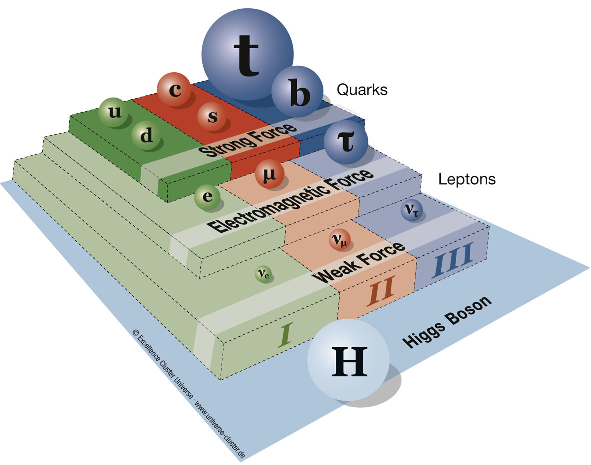
\includegraphics[width=\hugefigwidth]{chap_SMAndQGP_figures/StandardModel}
%  \caption[Standard Model]%
%  {Standard Model Figure}
%  \label{fig:SM}
%\end{figure}


%\begin{figure}
%  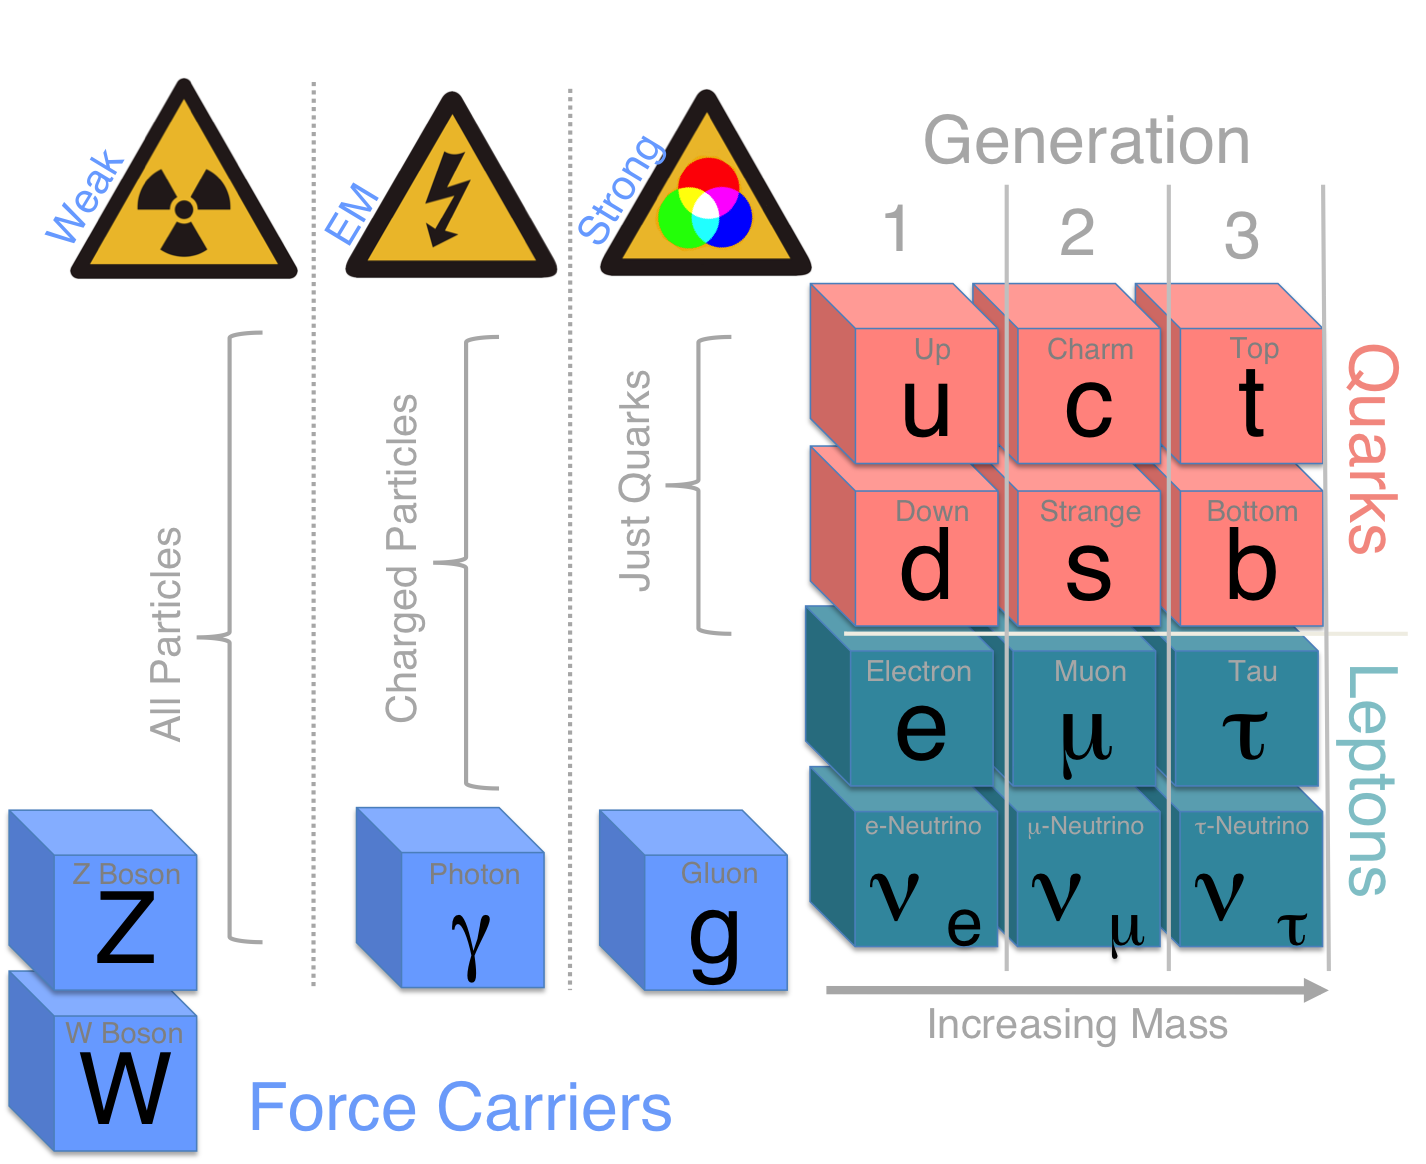
\includegraphics[width=\hugefigwidth]{chap_SMAndQGP_figures/SM_Fig4}
%  \caption[Standard Model 2]%
%  {Standard Model Figure 2}
%  \label{fig:SM2}
%\end{figure}



\begin{figure}
  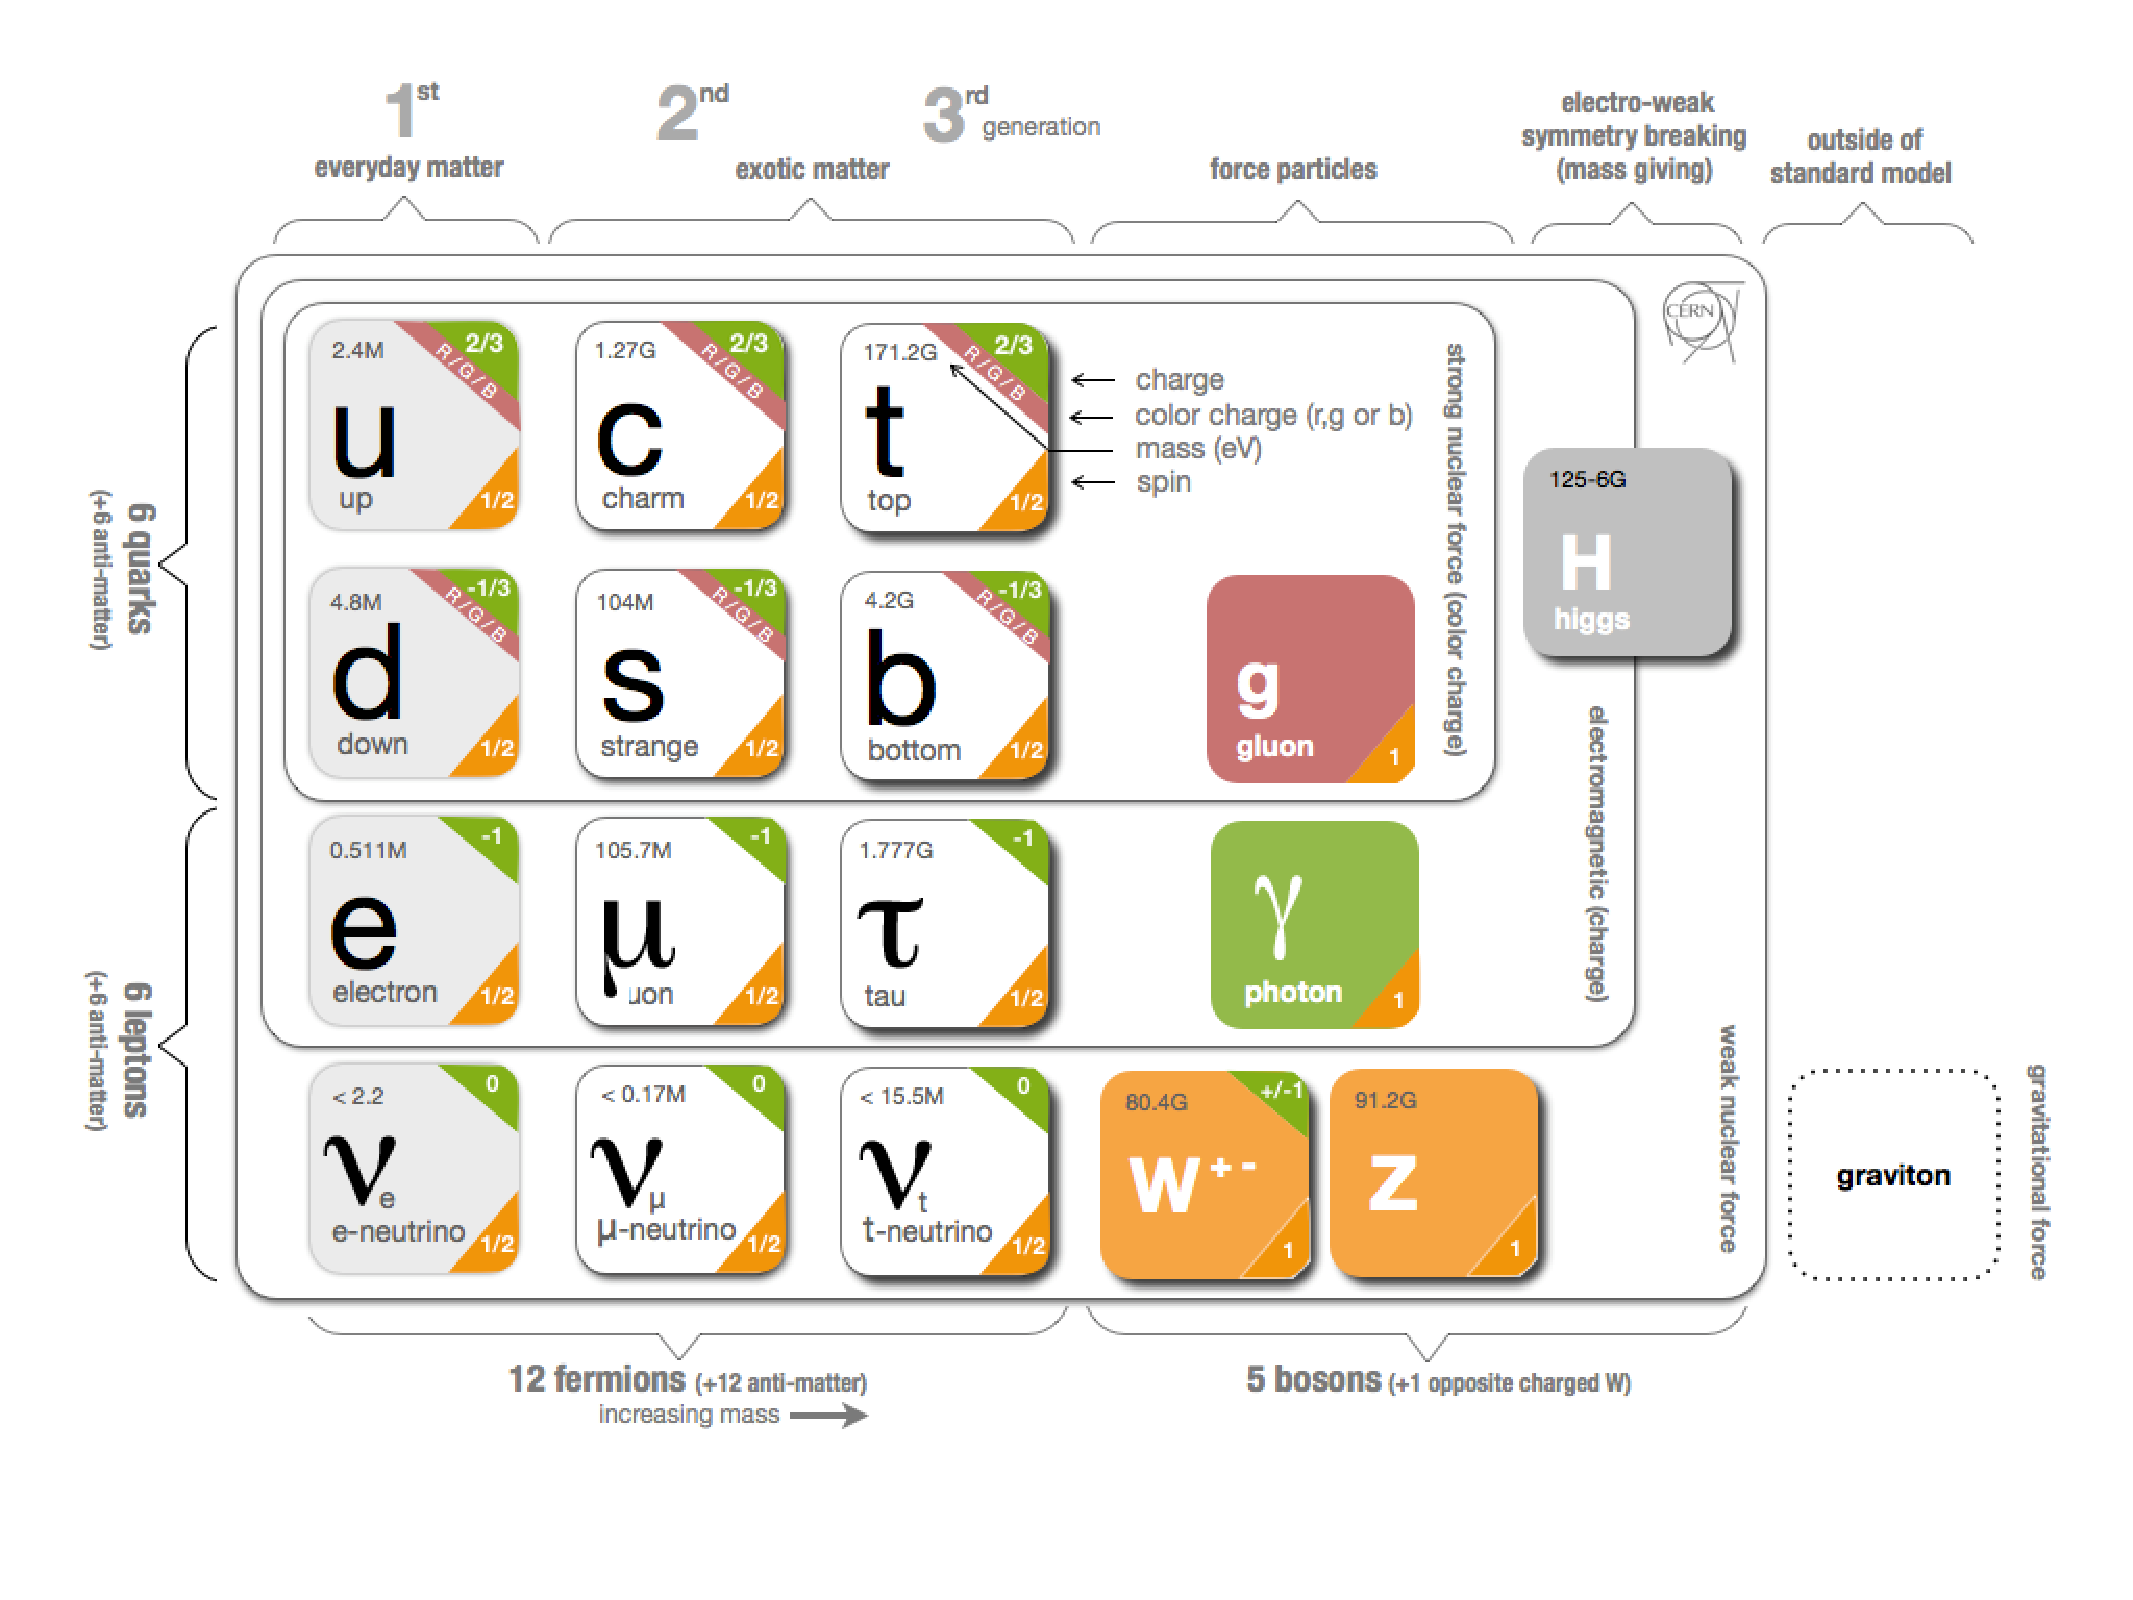
\includegraphics[width=\hugefigwidth]{chap_SMAndQGP_figures/Standard_model_infographic}
  \caption[Standard Model leptons and bosons]%
  {Standard Model leptons and bosons.}
  \label{fig:SM}
\end{figure}




\begin{table}[bht]
\caption[]{Boson properties}
\label{tab:StandardModelBoson}
\begin{tabular}{llll}
Name                                  &Force           &Electirc Charge         &Mass [GeV/c$^2$] \\
Symbol                                &Range(m)        &Color charge            &Strength        \\

\hline
Photon                                &Electromagnetic   &0                        &0                        \\
$\gamma$                              &$\infty$          &0                        &$\alpha$=$\frac{1}{137}$  \\

\hline
Gluon                                 &Strong            &0                        &0                        \\
g                                     &$10^{-15}$          &8 colored gluons         &$\alpha_s\,~$1, at high energy $\alpha_s \rightarrow$ 0\\

\hline
Z Boson                               &Weak               &0                        &91.187                        \\
Z$^0$                                 &$10^{-18}$           &0                        &$\alpha_z\,=\,10^{-6}$         \\

\hline
W Boson                              &Weak                &$\pm$1                   &80.399                        \\
W$^{\pm}$                             &$10^{-18}$            &0                        &$\alpha_W\,=\,10^{-6}$         \\
\end{tabular}
\end{table}




\subsection{Quantum Chromodynamics}

Quantum chromodynamics (QCD) \cite{QCD1,QCD2,QCD3,QCD4} is the field theory describing the
strong interactions of colored quarks and gluons. Color charge comes in three versions
(red, green and blue) that form a fundamental representation of the SU(3) group,
and is carried by both the quarks and gluons. Analogous to electric charge in quantum
electrodynamics (QED) \cite{QED1,QED2}, color charge is conserved in QCD, but since the gluons
carry color charge, they can interact with other gluons. This is not possible in QED,
as photons do not carry electric charge. The existence of self-coupling in QCD has
important implications for the scale dependence of the strong coupling.
In quantum field theory, the coupling constant describing the interaction between
two particles is an effective constant, which is dependent on the energy$-$scale Q$^2$ of
the interaction. In QED this dependence is only a weak one; in QCD, however, it
is very strong. The reason is the self-coupling of the gluons. The dependence of the
strong coupling constant $\alpha_s(Q^2)$ on Q$^2$ is known as a running coupling constant. In
perturbative QCD (pQCD), a first-order approximation yields:

\begin{equation}
\label{eq:QCD}
\alpha_s(Q^2) = \frac{1}{\beta_0\,ln(\frac{Q^2}{\Lambda^{2}_{QCD}})},\,\mbox{where}\,\beta_0 = \frac{33-n_f}{12\pi}
\end{equation}

Here, n$_f$ denotes the number of quark types with mass below Q$^2$, and $\Lambda_{QCD}$ represents
the characteristic scale of confinement. $\Lambda_{QCD}$ is determined by comparing predictions
with experimental data and is found to be on the order of 250 MeV \cite{QCD5}.


\begin{figure}
  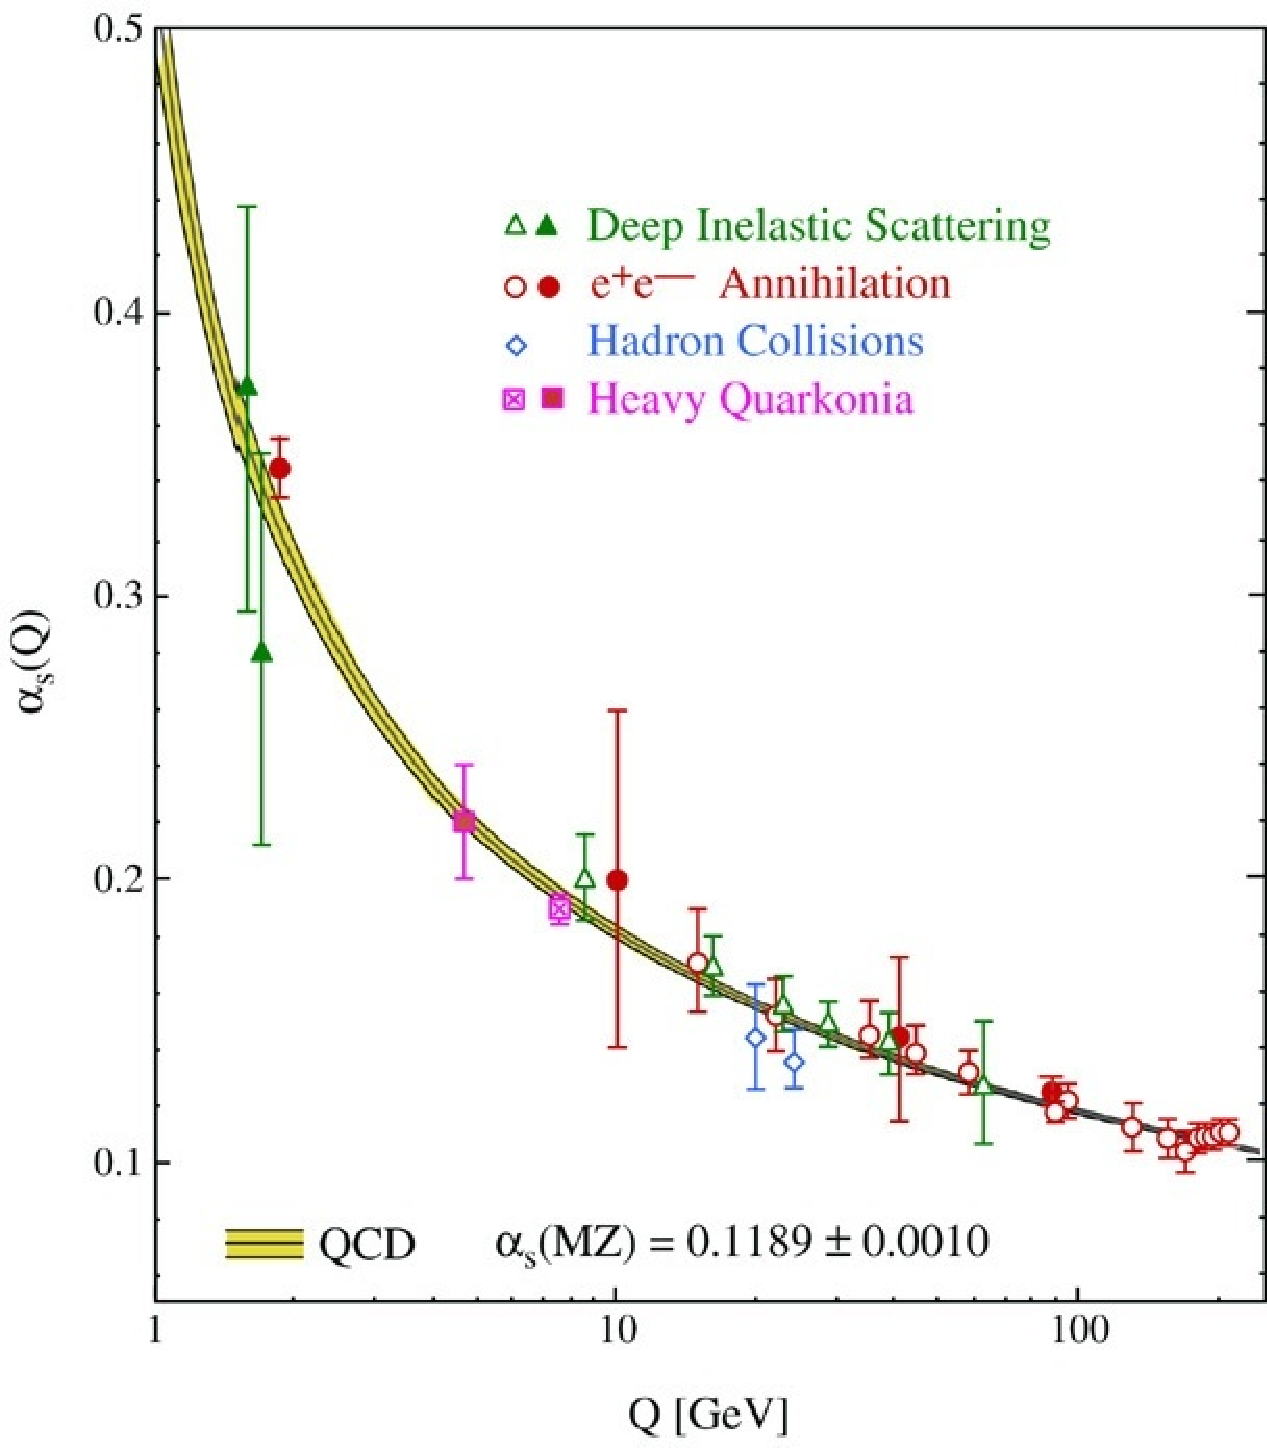
\includegraphics[width=\largefigwidth]{chap_SMAndQGP_figures/QCDAlpha_Prog}
  \caption[]{Figure shows a compilation of the values for $\alpha_s$, derived from many different experiments, and for different momenta Q of 
    the exchanged gluons. Gluon momentum is measured in GeV/c, and a logarithmic scale has been used to allow to show a bigger range of 
    values.}
  \label{fig:QCDAlpha}
\end{figure}



The Q$^2-$ dependence of the coupling strength corresponds to a dependence on quark
separation. For very small distances and corresponding high values of Q$^2$, the strong
coupling decreases, vanishing asymptotically as Q$^2\,\rightarrow\,\infty$ \ref{fig:QCDAlpha}. 
In the limit Q$^2\,\rightarrow\,\infty$, quarks
can be considered to be ``free''; this phenomenon is called asymptotic freedom. In
contrast, at large distances, the strong coupling increases substantially so that it is
not possible to detach individual quarks from hadrons. This phenomenon is called
confinement. In this regime, perturbation theory breaks down.
Quarks and gluons are not seen in experiments. Instead, they turn into hadrons,
which are observed in the detectors. This process is called hadronization. Hadronization
of quarks happens at a later time (t $\sim\,\frac{1}{\Lambda_{QCD}}$)
than the production process (t$\sim\,\frac{1}{Q}$). This is why the calculations 
of hadronic cross sections can be factorized into perturbative and non-perturbative parts.


\subsection{High Temperature QCD Matter}

The behavior of QCD at high temperatures or densities has long been of interest. In the first
few microseconds after the Big Bang, the universe would have had an enormous energy density, and
hence a very high temperature. It is expected that at such temperatures the component quarks
and gluons of normal hadronic matter have enough energy that they are no longer confined to their
usual bound states. This results in a phase transition between normal matter and a new state,
known as the Quark-Gluon Plasma (QGP) in analogy to electromagnetic plasmas in which the
electrons and ions are freed of their atomic bound states. A corresponding phase diagram can be
constructed, as shown in Figure \ref{fig:QCDPhaeDiagram}, which includes normal nuclear and hadronic matter, as well
as the QGP phase. In addition, other phases are expected to exist at higher net baryon chemical
potential, such as in neutron stars.


\begin{figure}
  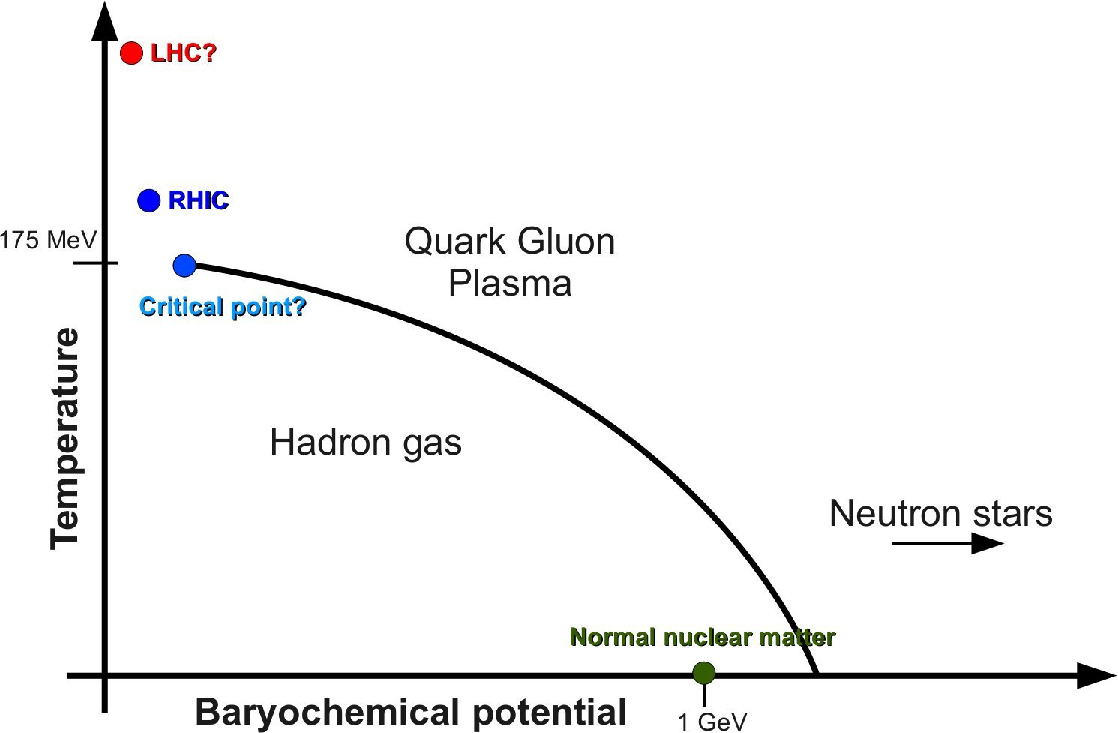
\includegraphics[width=\hugefigwidth]{chap_SMAndQGP_figures/QCDphasediagram1}
  \caption[QCD Phase diagram]
  {QCD phase diagram}
  \label{fig:QCDPhaeDiagram}
\end{figure}


\begin{figure}
  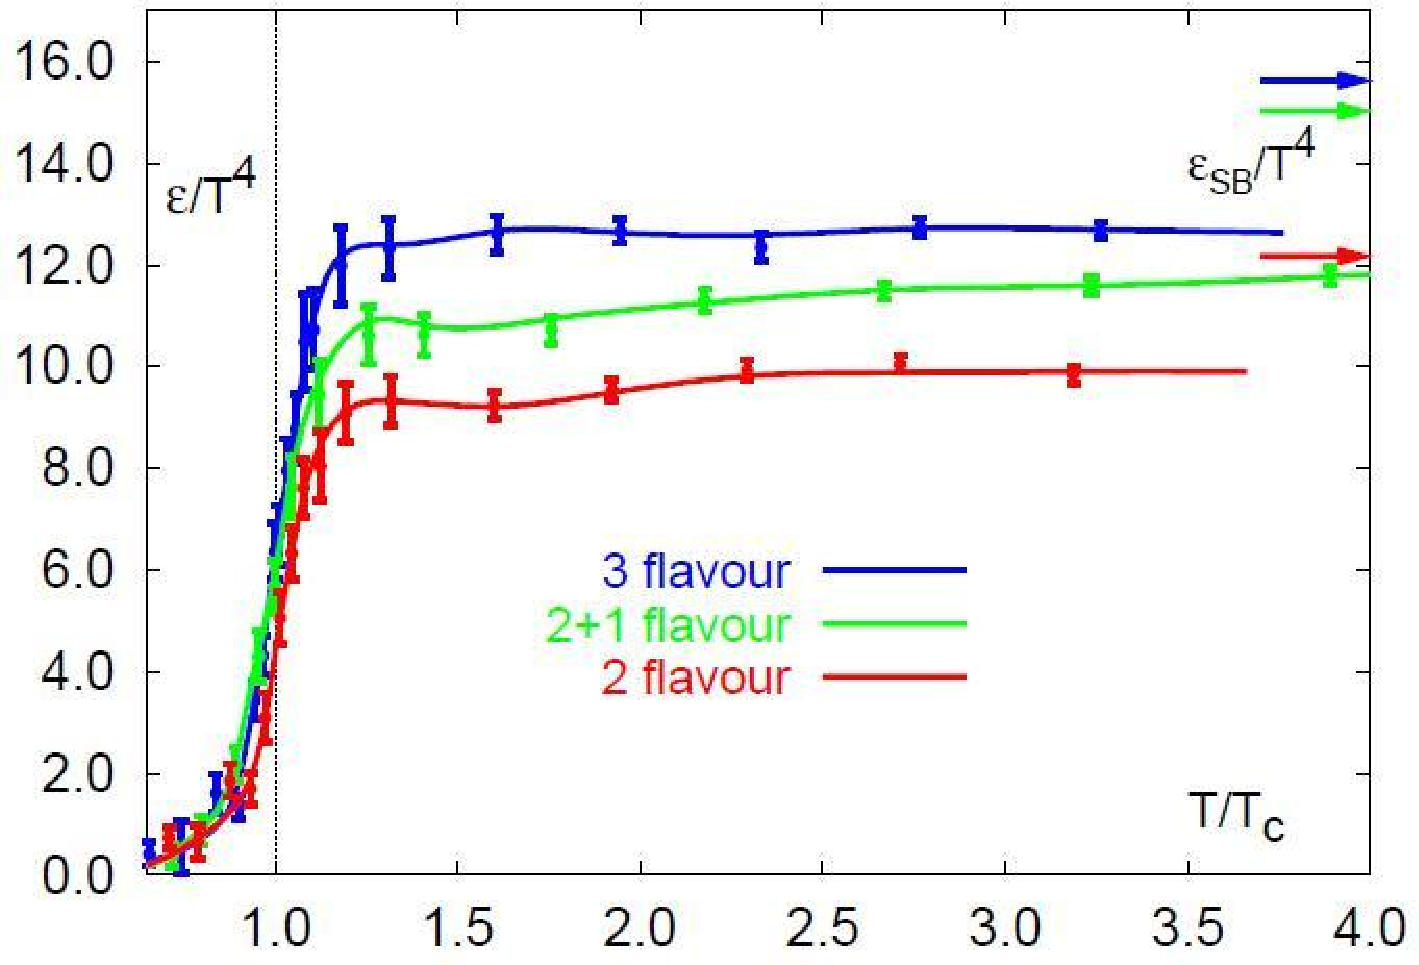
\includegraphics[width=\hugefigwidth]{chap_SMAndQGP_figures/LatticeQCD}
  \caption[QCD Phase diagram]
  {Energy density in units of T$^4$ as calculated in lattice QCD as calculated in \cite{LQCD1}. The
sharp rise at T$\sim$ T$_c$ corresponds to the phase transition to the QGP. On the right side the energy
density of a simple Stefan-Boltzmann gas of partons (as calculated in the text) is labeled.}
  \label{fig:LatticeQCD}
\end{figure}


Unfortunately, the QGP near the transition temperature is an inherently non-perturbative
regime, and other methods must be used to perform calculations. One way around this difficulty
is to perform numerical calculations using lattice QCD, which makes use of a Euclidean spacetime
grid to calculate the path integral of the QCD partition function. From there statistical and
thermodynamic properties such as temperature and free energy can be calculated.

Recently lattice QCD has been used to examine the phase transition to a QGP. It was found
that the transition temperature is Tc $\sim$ 170 MeV. This happens to lie very close to the Hagedorn
temperature T$_H\,\sim\,$ 160 MeV, the limiting temperature in high-energy hadronic collisions, above
which only the entropy of the thermodynamic system is increased (i.e. the number of hadronic
states produced) \cite{Hagedron}.

In order to create such a state of matter in the laboratory, heavy nuclei are collided at
relativistic velocities such that a portion of the large kinetic energy is converted to thermal energy.
The temperature dependence of the energy density can be naively calculated by assuming
the QGP is a Stefan-Boltzmann gas of massless, non-interacting particles \cite{WongBook,RamonaBook}. The partition
function for fermions $(-)$ and bosons $(+)$ is:


\begin{equation}
\label{eq:QCDPartFunc}
\mbox{ln Z(T,\mu,V)}=\frac{gV}{2\pi^2T}\int_{0}^{\infty}\frac{dk\,k^4}{3E}\, [ \frac{1}{e^{(E-\mu)/T}\pm1} + \frac{1}{e^{(E+\mu)/T}\pm1} ]
\end{equation}

If we assume that the number of quarks and anti-quarks are equal, then it can be shown that $\mu$=0.
For gluons (or other bosons), this becomes

\begin{eqnarray}
\label{eq:QCDPartFunc2}
\mbox{ln Z} &=  &g\frac{\pi^2}{90}VT^3 \,\,\mbox{(boson)}  \nonumber  \\
            &=  &g\frac{7\pi^2}{720}VT^3 \,\,\mbox{(fermions)} \nonumber \\
\end{eqnarray}

Now, since energy density is

 
\begin{eqnarray}
\label{eq:QCDEnDens}
\epsilon &= &(\frac{T^2}{V})( \frac{\delta \mbox{ln Z}}{\delta T}) \nonumber 
\end{eqnarray}

We can calculate

\begin{eqnarray}
\epsilon &= &(g_b + \frac{7}{8}g_f) \frac{\pi^2}{30} T^4 \\ 
\end{eqnarray}

where g$_{b,f}$ are the degeneracy numbers of the bosons,fermions as calculated below for gluons and
quarks+antiquarks:

\begin{eqnarray}
g_b &= &g_{gluon}             =(\mbox{(8 color states)(2 spin)}  \nonumber \\
g_f &= &g_{q}+g_{\overline{q}}   = \mbox{2(3 color)(2 spin)(n flavor)}    \nonumber \\
\end{eqnarray}

This gives us

\begin{eqnarray}
\epsilon &= &37\frac{\pi^2}{30}T^4 \mbox{(2 quark flavour)}\nonumber \\ 
         &= &47.5 \frac{\pi^2}{30}T^4 \mbox{(3 quark flavour)}\nonumber \\
\end{eqnarray}


for the energy density of a gas of massless partons.

Using lattice QCD it is possible to perform a more realistic calculation of the energy density.
Figure \ref{fig:LatticeQCD} shows such a calculation of the energy density \cite{LQCD1}. 
At sufficient temperature, this result shows the same T$^4$-scaling of the plasma energy density 
as calculated above. It should be noted that the calculation plateaus at $\sim$80$\%$ of the 
Stefan-Boltzmann gas of non-interacting partons. This
has sometimes been taken as evidence that the plasma weakly-interacting, but other calculations
have shown that even a strongly-interacting plasma could approach this limit \cite{LQCD2}.

As the medium expands and cools, it passes through several phases, as shown in Figure \ref{fig:HICollWhite}.
First hadronization will occur once the temperature becomes low enough that partons are confined
again. Next, kinetic freeze-out occurs when the expanding hadrons are too sparse to interact with
one another. At this point they will continue along their trajectories to be experimentally observed.
In order to extract any properties of the QGP medium, the evolution through other phases must
be accounted for as well. Hadronization in particular is not understood very well.

Topics of interest for the produced medium include the amount of thermalization of the
medium, how strongly-interacting the medium is, the nature of the phase transition itself, among
others.

Unfortunately, we are limited in our capabilities to experimentally study the properties of the
medium, due to its exceedingly short lifetime. Because of this we are constrained to probes that are
produced in the same collision as the medium, such as jets or heavy quarks from a hard scattering.


\begin{figure}
  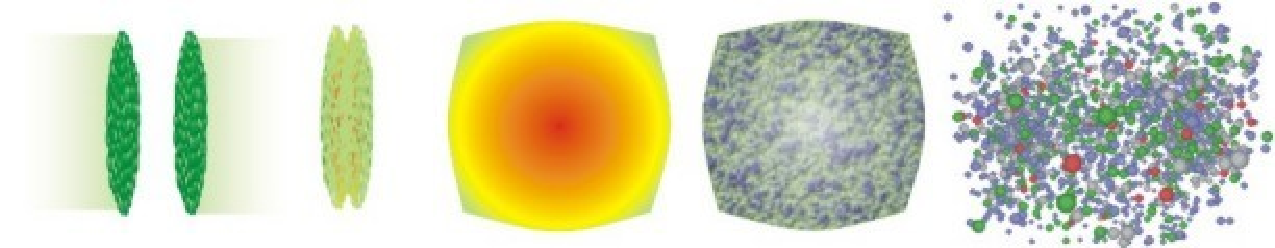
\includegraphics[width=\hugefigwidth]{chap_SMAndQGP_figures/HICollisions_White}
  \caption[HeavyIon Collisions]%
  {HI Collisions}
  \label{fig:HICollWhite}
\end{figure}

To understand the experimental measurements of these probes, however, we must understand their
initial production cross sections as well.


Our available probes and observables for studying the QGP medium include:
\begin{itemize}
 \item Elliptic flow of particles to study on the shear viscosity/entropy of the medium.
 \item Jet modification due to in-medium scattering and energy loss.
 \item Heavy quark flow as a measure of the medium thermalization.
 \item Hanbury-Brown-Twiss (HBT) interferometry to evaluate the distribution of matter.
 \item J/$\psi$ suppression above the QGP transition temperature as a signature of deconfinement.
 \end{itemize}

For a detailed review of experimental and theoretical status, see \cite{QGPThRev,QGPExpRev}.


To expand upon the last bullet item in the list, the QGP is expected to exhibit screening of the
interactions between color charges, similar to Debye screening of electric charges in electromagnetic
plasmas. Calculations of the screening length near the transition temperature have led to the
conclusion that the J/$\psi$  meson (a charm-anticharm bound state) is the right size to have its
constituent quarks Debye-screened from one another just above T$_c$. On the other hand  J/$\psi$ 
suppression is also affected by other effects like Cold Nucler Matter effect and recombination of
uncorelated charm-anticharm quark pair. It is observed that relative supperession $\Upsilon$ family
(bound state of b$\overline{b}$) can more roubest signature of Quark Gluon Plasma.  
 

%\begin{figure}
%  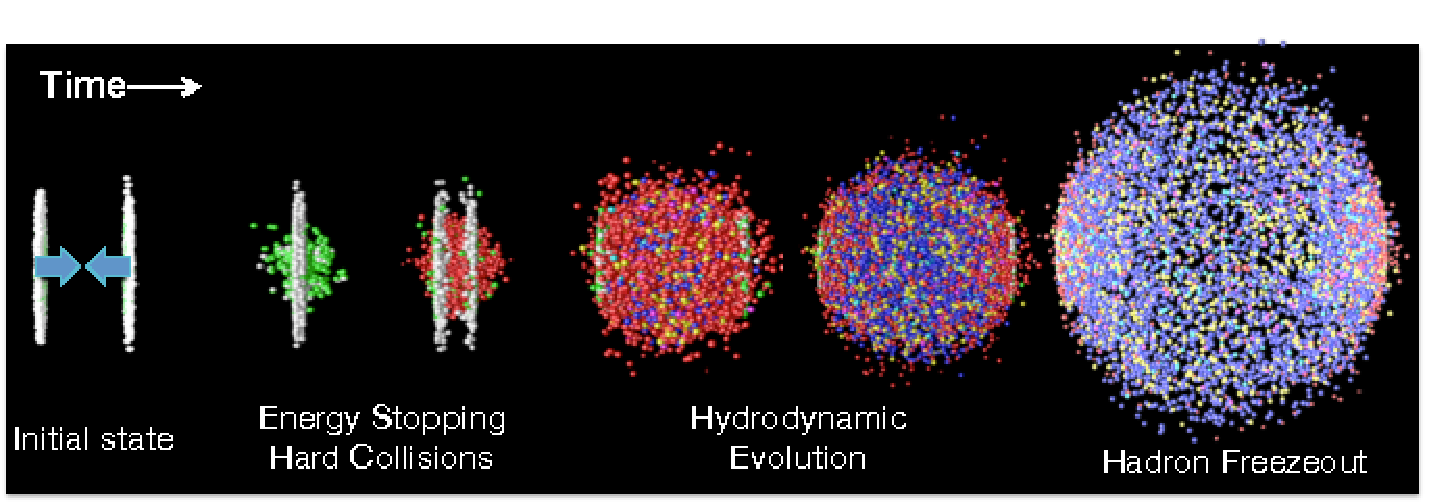
\includegraphics[width=\hugefigwidth]{chap_SMAndQGP_figures/black_heavy_ion_evolution}
%  \caption[HeavyIon Collisions time evolution]%
%  {HI Collisions time evolution}
%  \label{fig:HICollBlk}
%\end{figure}



%\begin{figure}
%  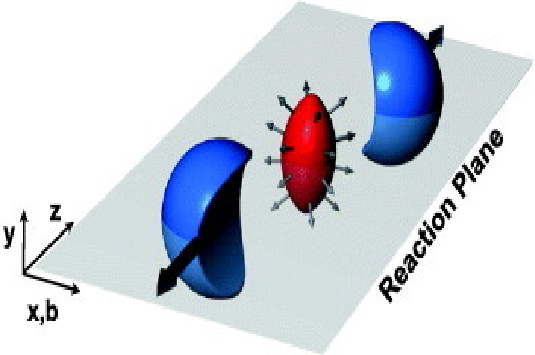
\includegraphics[width=\hugefigwidth]{chap_SMAndQGP_figures/ElipticFlow2}
%  \caption[Elitical flow in HI Collision]
%  {Elitical flow in HI Collision (v$_2$)}
%  \label{fig:V2}
%\end{figure}






  \chapter{Quarkonia production and properties in Hot and dense matter}
\label{QuarkoniaInQGP}

\section{Quarkonia}

\subsection{The discovery of quarkonia}
In November 1974 a narrow resonance at 3.1 GeV/c$^2$ in the $\mu^+\mu-$ invariant
mass spectrum was observed \cite{JPsiDiscovery,DDbarMixing} in proton-beryllium and 
electron positron collisions. The particle was named J/$\psi$. At that time the world was
expected to consist of up, down and strange quarks plus electrons and muons.
In addition a fourth quark was predicted by the Glashow-Iliopoulos-Maiani
(GIM) mechanism \cite{GIM_CharmPred}. Soon after the first observation it became clear that
the newly discovered particle consisted of the predicted quark species, the so
called charm quarks. This discovery added a new particle to the fundamental
building blocks of nature. In addition the description of the small width of the
observed peak, 93.4$\pm$1.2 keV \cite{Rev_PartPhysics}, was one of the first big successes of QCD, a
theory still relatively new at that time. Three years later another sharp resonance
in the dimuon spectrum was discovered in proton-nucleus collisions \cite{YDiscovery},
the $\Upsilon$. This time the surprise in the physics community was not as large since
the third lepton, the $\tau$, was discovered in the mean-time and for symmetry
reasons one expected a third quark family. The heaviest quark, the top quark,
was discovered in 1995 \cite{TopDiscovery}. This discovery completed the three quark families.
Up, down and strange quarks are commonly called light quarks, while the
charm, bottom and top are referred to as heavy quarks. The bound state of
these heavy quarks with their corresponding anti-particle is called quarkonia.
The top quark cannot form a bound state, due to its short lifetime of less than
10$^{-24}$s. A heavy quark-anti-quark pair is able to form more then one bound
state. Apart from the J/$\psi$  and the $\Upsilon$ more higher excited states exist, forming
the so-called J$\psi$  and the $\Upsilon$ families as shown at Figure 
\ref{fig:JPsiFamily} and \ref{fig:UpsilonFamily} \cite{Rev_PartPhysics}.

\begin{figure}
  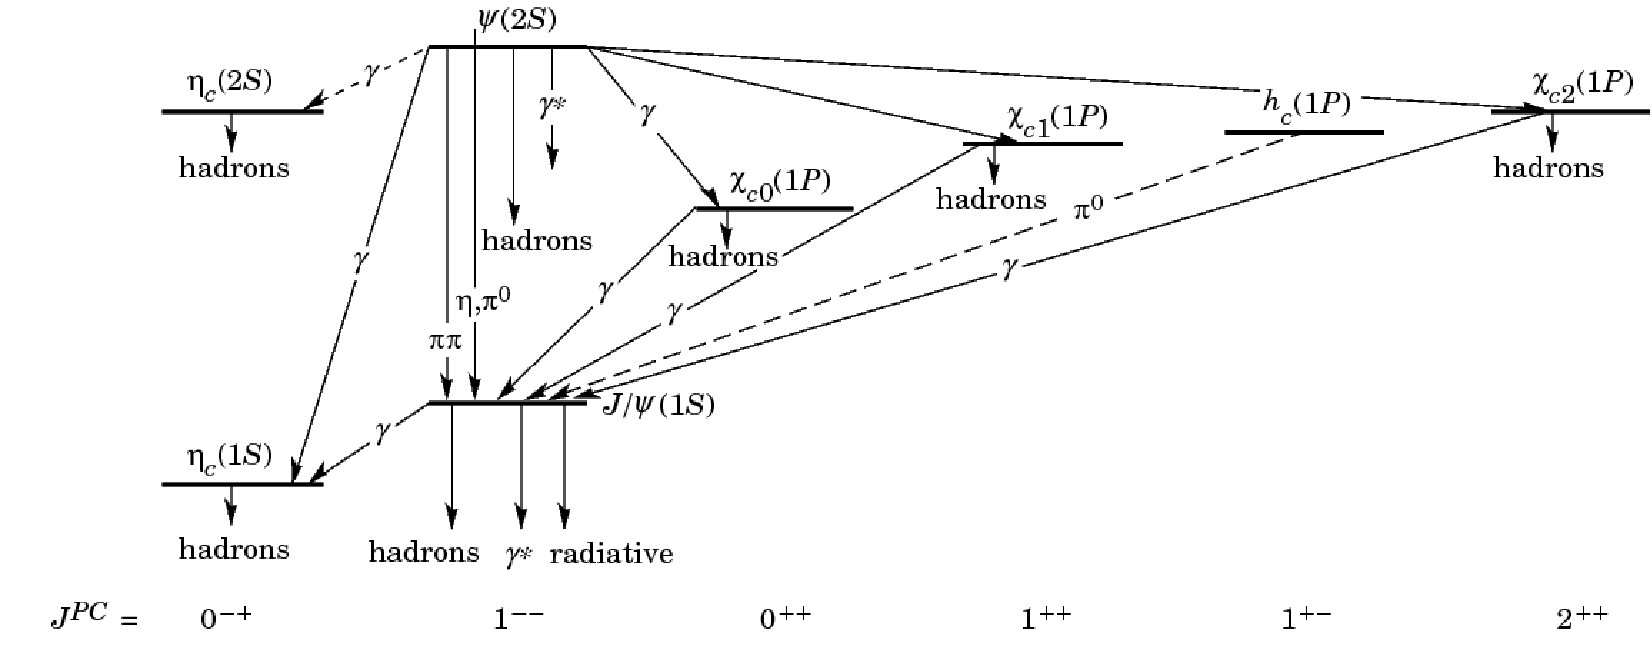
\includegraphics[width=\hugefigwidth]{chap_QuarkoniaSurvey_figures/JPsiFamily}
  \caption[J/$\psi$ family]
   {Different bound states of charm and anti-charm quark.}
   \label{fig:JPsiFamily}
\end{figure}



\begin{figure}
  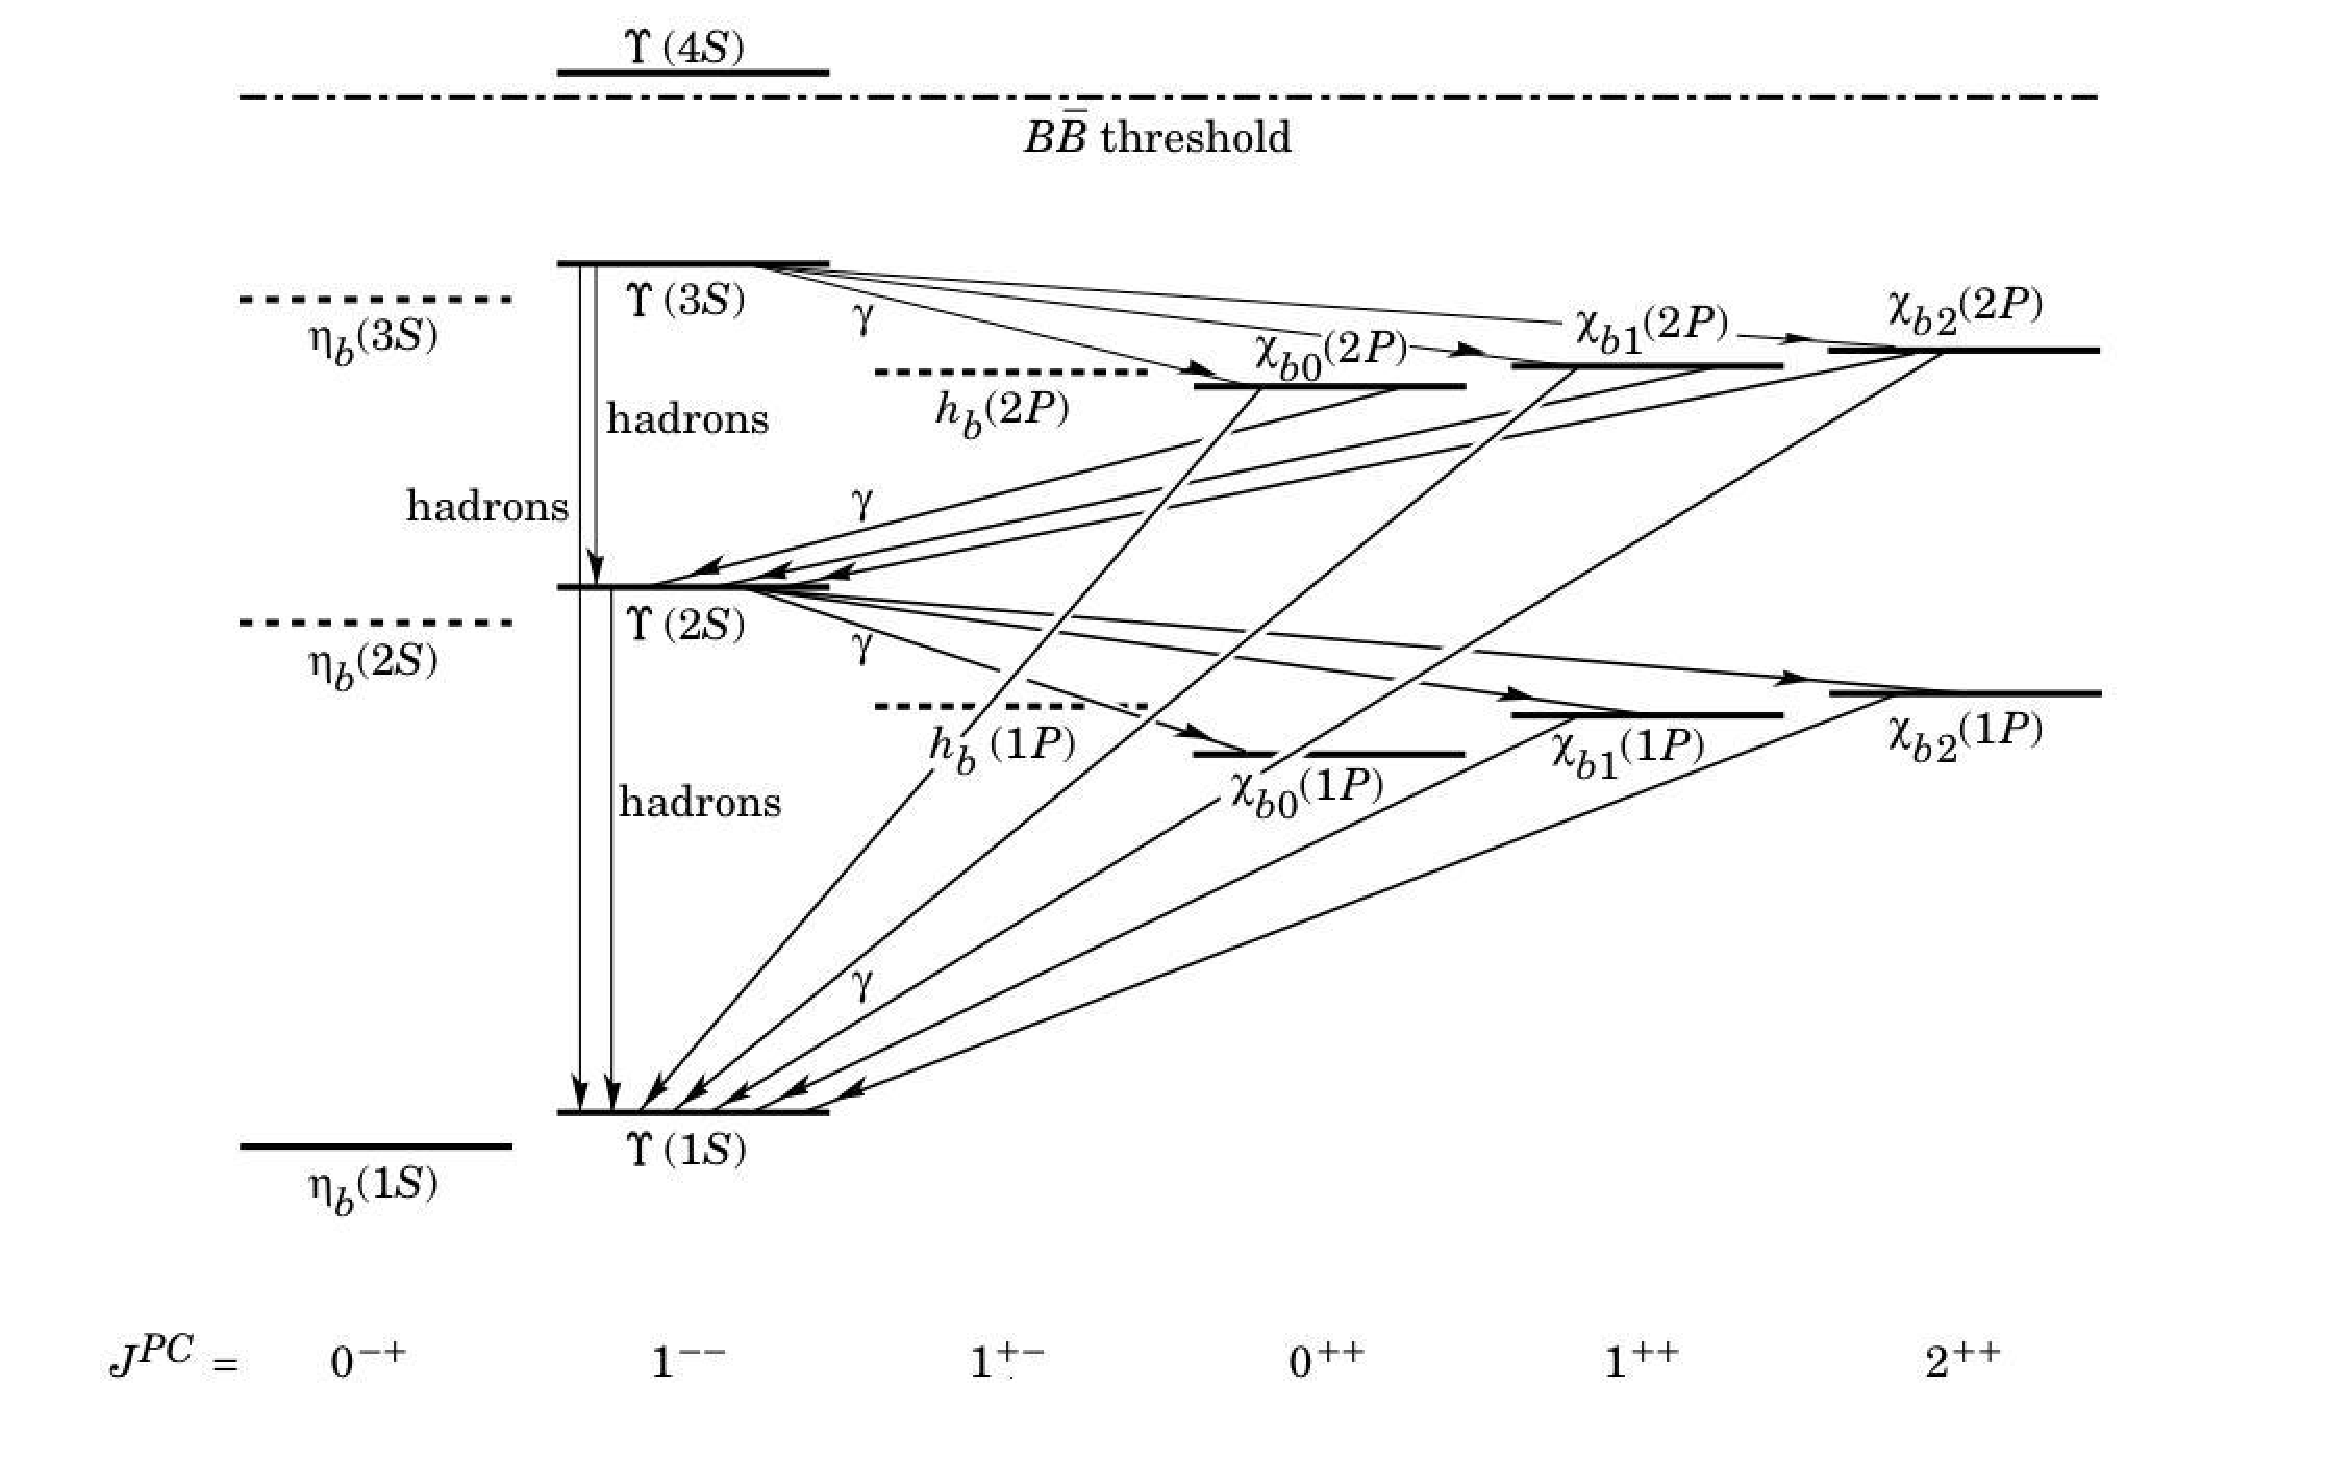
\includegraphics[width=\hugefigwidth]{chap_QuarkoniaSurvey_figures/UpsilonFamily}
  \caption[$\Upsilon$ family]
   {Different bound states of beauty and anti-beauty quark.}
   \label{fig:UpsilonFamily}
\end{figure}


\subsection{Quarkonium production}
In general one can subdivide the production process into two major parts
\begin{itemize}
\item Production of a heavy quark pair in hard collisions.
\item Formation of quarkonia out of the two heavy quarks.
\end{itemize}

{\bf Production of a heavy quark pair in hard collisions}\\
Due to the high mass of the heavy quarks (m$_{charm}\,\sim$ 1.3 GeV/c$^2$, m$_{bottom}\,\sim$ 4.7 GeV/c$^2$) 
the first process can happen only during the first phase of a collision. Only at that
time the elementary collisions with sufficiently high momentum transfers to
create such high masses take place. For this reason the heavy quark production
is a hard process that can be treated perturbatively. In next-to-leading order
(NLO) calculations the available experimental data at different energies and
collision system \cite{Baines,Ramona_Paper1} were described. The obtained parameters were then
used to predict the total production cross section in proton-proton collisions at
LHC energies. The charm production cross section is predicted to be 6.3 mb.
and the bottom production cross section 0.19 mb \cite{Ramona_Paper2}. To obtain upper and
lower limits for this cross sections the parameters have been varied leading to
a relatively large range for the charm production cross section of 4$-$15 mb and
0.08$-$0.34 mb for the bottom production cross section. \\
{\bf Formation of quarkonia out of the two heavy quarks}\\
The second part,namely the formation of quarkonia out of the quark-anti-quark pair can a
priori not be treated perturbative. Due to the high quark masses and the
small relative velocities in the quarkonium system, the formation can be described
using non-relativistic QCD (NRQCD). This allows the factorization
into a perturbative small-range and high-momentum part and a long-ranged
and low-momentum part. In the past years especially three models were developed,
namely the Color Singlet Model (CSM) \cite{CSM1, CSM2}, the Color Octet
Model \cite{COM1, COM2, COM3} and the Color Evaporation Model (CEM) \cite{CEM1, CEM2, CEM3}
\begin{itemize}
\item Color Singlet Model (CSM): The quarkonia formed out of the two quarks
has to be color neutral. Since in principal the two heavy quarks are not
necessarily carriers of one color and the corresponding anti-color, the
combination might be colored \footnotemark. The Color Singlet Model rejects all color

\footnotetext[1]{The symmetry group of QCD is the SU(3). The colors are triplet, R, G, B and their anti-color
$\overline{R},\overline{G}$ and $\overline{B}$  triplets one can form 3 $\bigotimes$ 3 = 8 $\bigoplus$ 1 
combinations, one octet and one singlet. The color octet states are R$\overline{G}$, R$\overline{B}$, 
G$\overline{R}$, G$\overline{B}$, B$\overline{R}$, B$\overline{G}$, 
$\sqrt{\frac{1}{2}}(R\overline{R}-G\overline{g})$, $\sqrt{\frac{1}{6}}(R\overline{R}+G\overline{G}-2B\overline{B})$,
. The color singlet is $\sqrt{\frac{1}{6}}(R\overline{R}+G\overline{G}+B\overline{B})$.}

octet states, in the NRQCD factorization the produced quarkonium has
the same quantum numbers as the quark$-$anti-quark pair. Predictions by
the CSM for the production of quarkonium in pp at Tevatron underestimated
the data by an order of magnitude, thus it was clear that the
color octet states cannot be neglected.

\item Color Octet Model (COM): The Color Octet model considers the octet
states, within the model quarkonium is only produced in an octet and
thus colored state. The pre$-$resonant colored state neutralizes its color
by the emission of a soft gluon. The Color Octet Model was able to
reproduce the production cross section but failed in the description of
the observed J/$\psi$  polarization \cite{CDF_Pola}.

\item Color Evaporation Model (CEM):As an expansion the Color Evaporation
Model was developed from the Color Octet Model. The evaporation of
the surplus color happens via many different processes, not only by the
emission of a soft gluon. This large number of processes results in a
relatively large number of parameters, that have to be determined by the
comparison to existing data. Although the tuning of the model to the
data works well, the large number of free parameters limit the predictive
power of the CEM. Nevertheless it is the best available approach for
describing the available measurements and it is used for the predictions
of the cross sections for LHC energies (see Figure \ref{fig:QuarkoniaCrossSection}).
\end{itemize}

\begin{figure}
  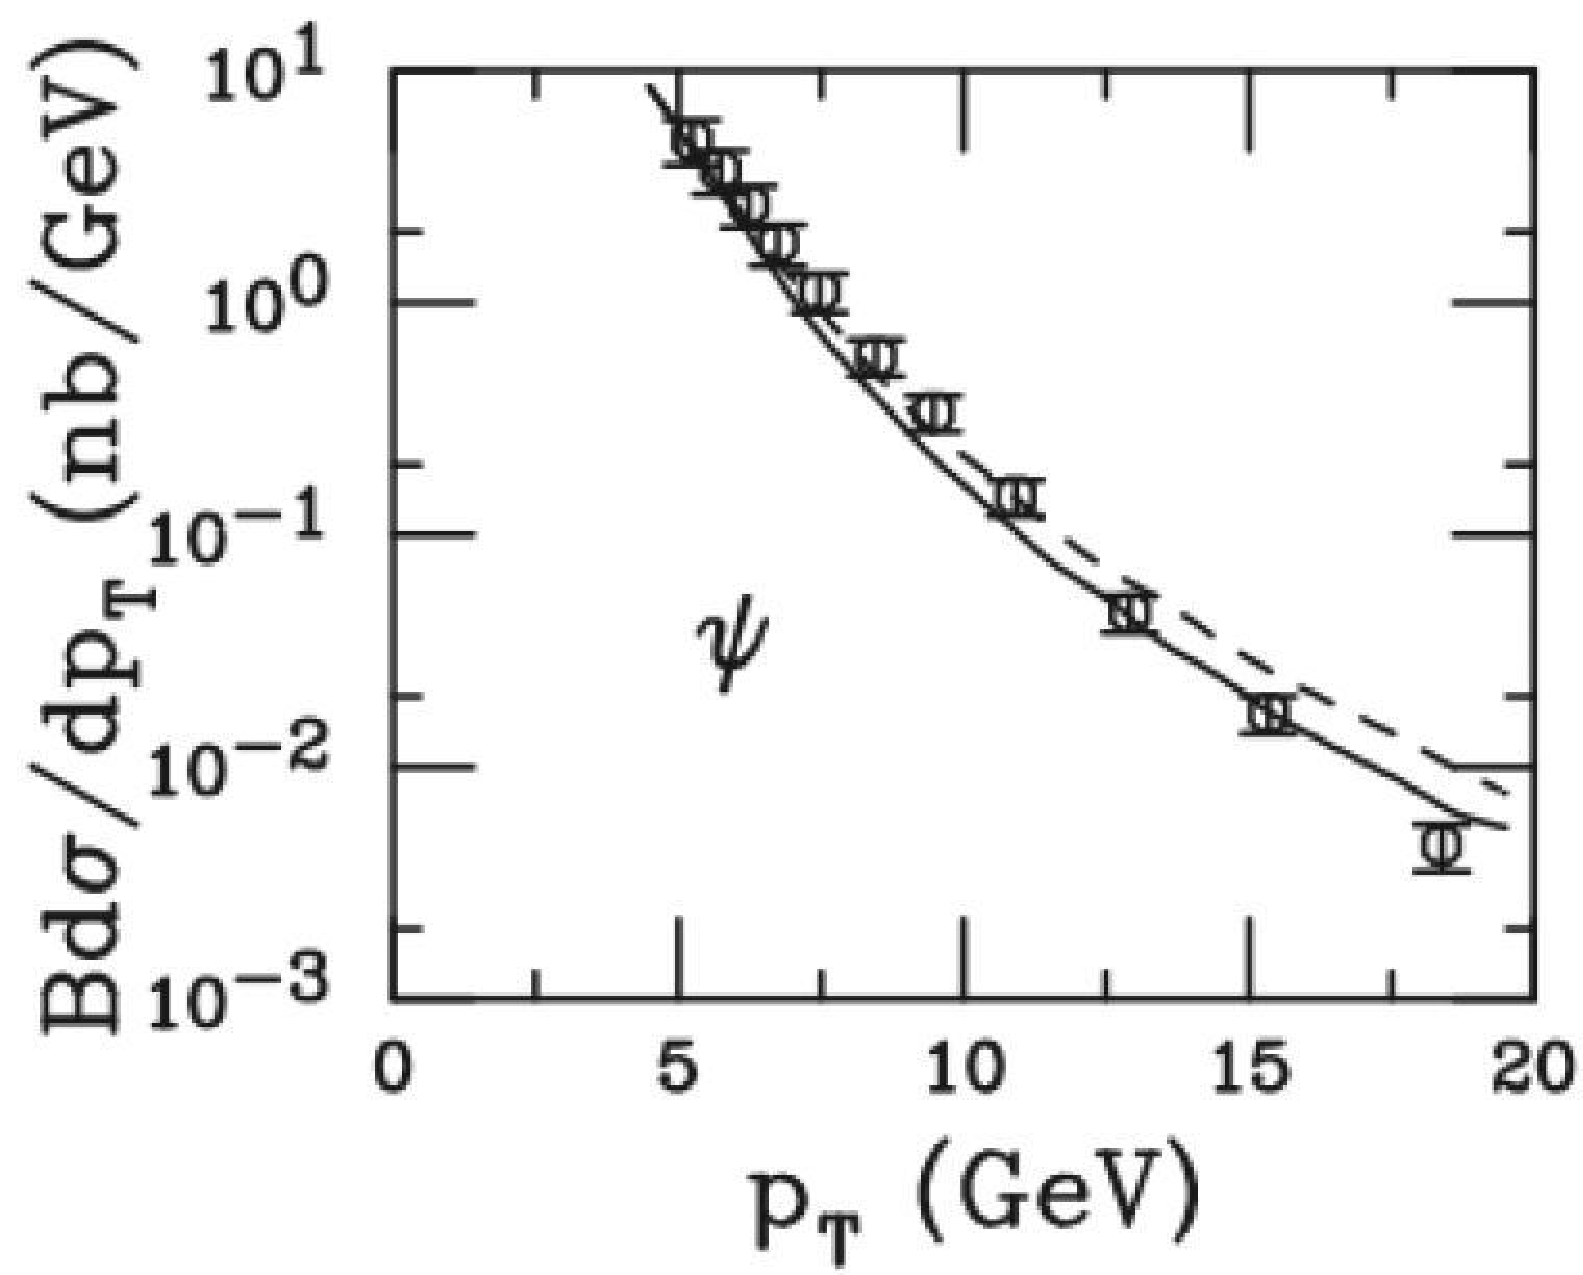
\includegraphics[width=\smallfigwidth]{chap_QuarkoniaSurvey_figures/JPsiCrossTevtron}
  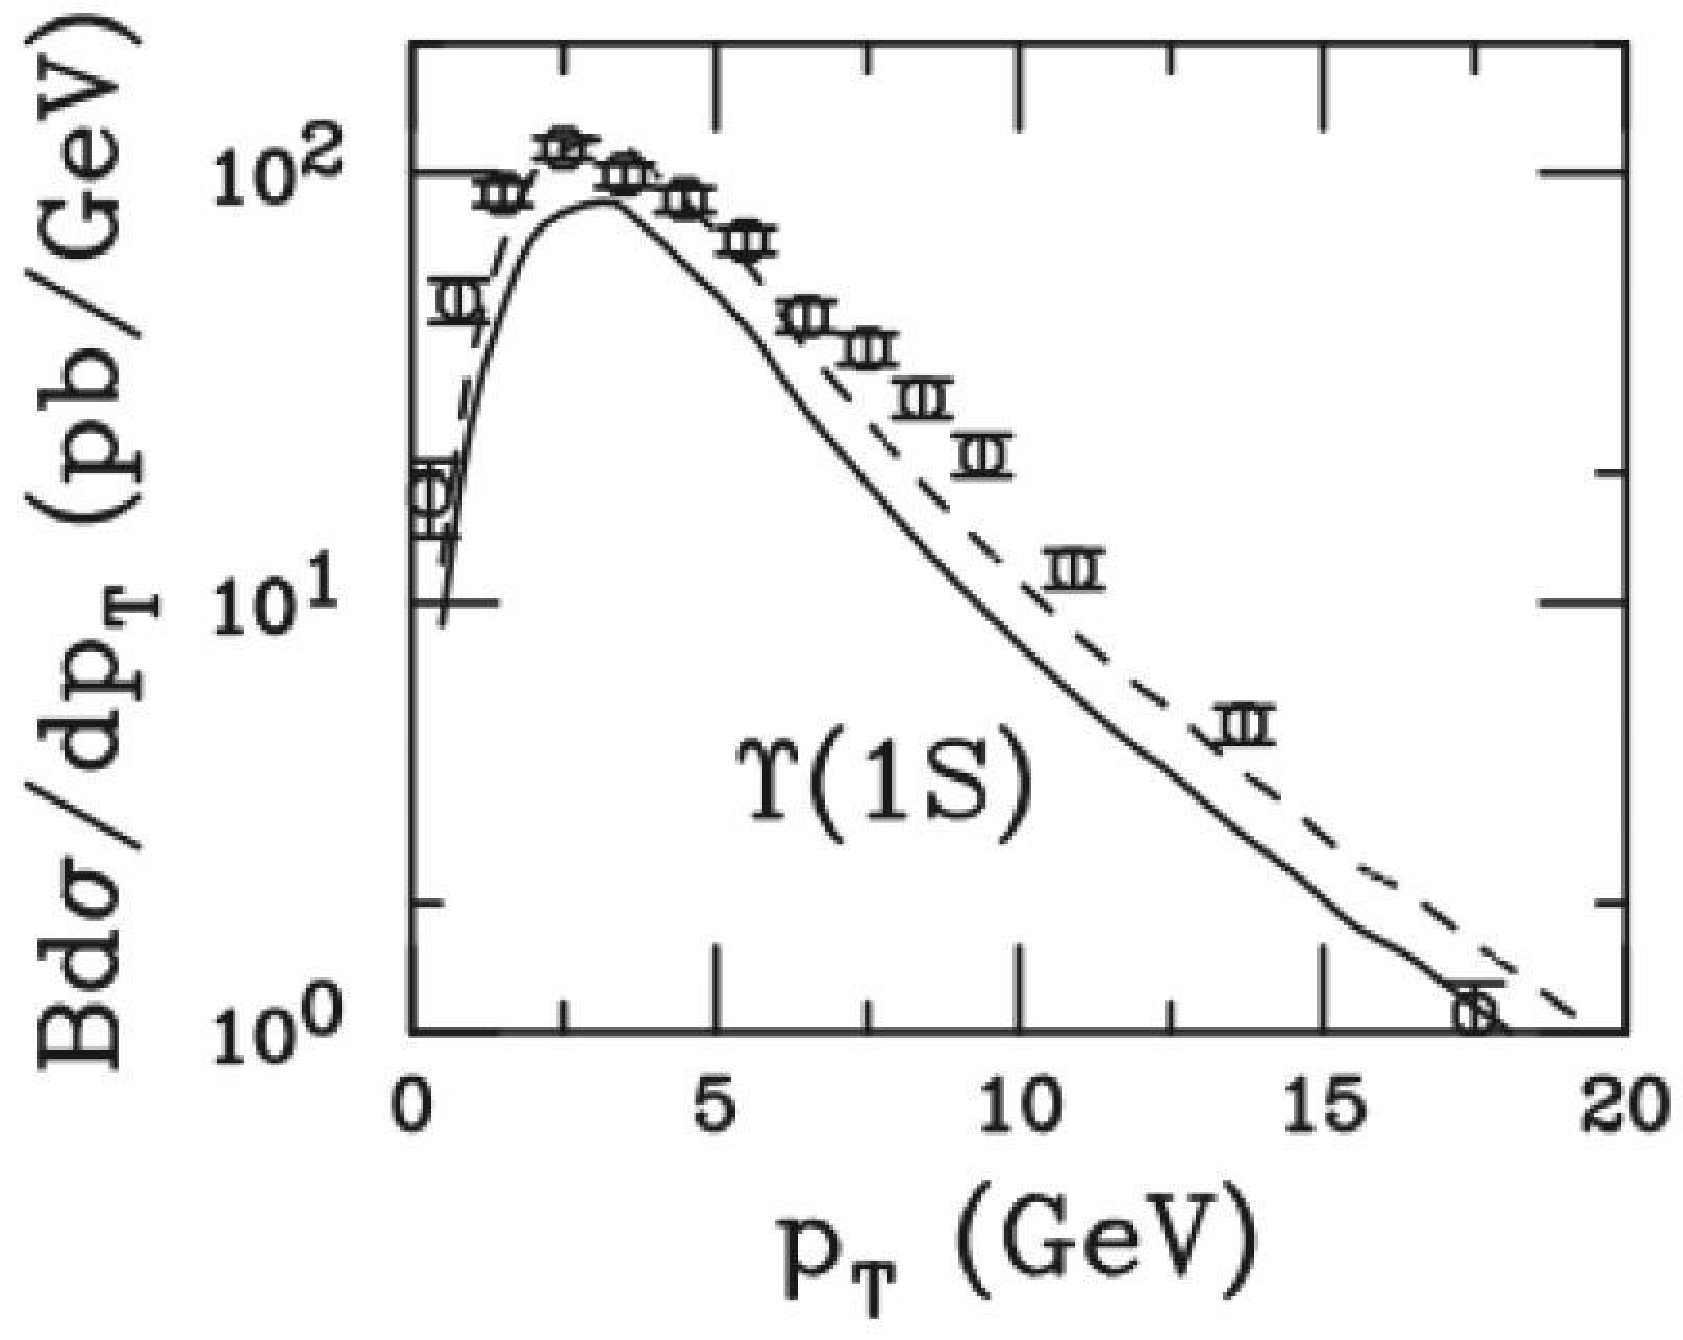
\includegraphics[width=\smallfigwidth]{chap_QuarkoniaSurvey_figures/YCrossTevtron}
  \caption[J/$\psi$ and $\Upsilon$ cross sections]
   {pT -dependent production of J/$\psi$ s and $\Upsilon$ s as measured by the
     CDF experiment \cite{CDF1, CDF2, CDF3} (circles) and compared to predictions by the
     Color Evaporation Model with two different parameter sets (solid+dotted).}
   \label{fig:QuarkoniaCrossSection}
\end{figure}



\subsection{Qualitative formation and decay times}
It is commonly accepted that at LHC energies the main production mechanism
of heavy quark and quarkonia is gluon fusion gg$\rightarrow$Q$\overline{Q}$. Gluons from the
nucleus wave function will form a Q$\overline{Q}$ pre$-$resonance in a characteristic (hard)
production time t$_p$
\begin{eqnarray}
t_p(p_t\, \gg\, m_Q) \approx \frac{E}{p_T^2} \approx \frac{1}{p_T},\,\,\,
t_p(p_t\, \leq\, m_Q)\sim \frac{1}{m_Q}
\end{eqnarray}
E being the pair energy. Thus, for p$_T \,\sim$ m$_Q$ the production time of
charm and beauty pre$-$resonance pairs would be about
\begin{eqnarray}
t_p(p_t\, \gg\, m_c) \sim 0.15 \mbox{fm/c},t_p(p_t\, \gg\, m_b) \sim 0.05 \mbox{fm/c}.   
\end{eqnarray}
The production time is then much smaller than 1 fm/c, and they are
formed at a relative distance 1/m$_Q\,\,\gg$ 1 fm. Then the Q$\overline{Q}$ pairs 
travel extremely close and to form a Q$\overline{Q}$ resonance they need to expand 
till the characteristic size of the resonance. It can be interpreted as the time 
the pair takes to decide which of the possible Q$\overline{Q}$ bound-states 
it will couple to (one with mass m1 or one with m2). This formation time can be calculated 
by means of \cite{Thews, Khar_Thews}
\begin{eqnarray}
t_f \simeq \frac{2E}{m_2^2 - m_1^2}
\end{eqnarray}

Thus the time a c$\overline{c}$ (b$\overline{b}$) pair takes to decide to form a J/$\psi$
($\Upsilon$) rather than a excited state

\begin{eqnarray}
t_f(J/\psi,E) \simeq \frac{2E}{m_{J/\psi}^2 - m_{\psi^{'}}^2} \nonumber \\
t_f(J/\psi,10 GeV) \simeq 1.0 fm/c.\nonumber \\
t_f(J/\psi,30 GeV) \simeq 3.0 fm/c. \nonumber \\
\end{eqnarray}

similarly for  $\Upsilon$ family

\begin{eqnarray}
t_f(\Upsilon,E) \simeq \frac{2E}{m_{\Upsilon}^2 - m_{\Upsilon^{'}}^2} \nonumber \\
t_f(\Upsilon,10 GeV) \simeq 0.36 fm/c.\nonumber \\
t_f(\Upsilon,30 GeV) \simeq 1.1 fm/c. \nonumber \\
\end{eqnarray}

The resonances formation times are thus much larger than the preresonances
production times. They increase with the particle momentum,
ranging from a fraction of fm/c to about 3 fm/c.
Later, the Q$\overline{Q}$ resonance being not a stable particle, it will decay with
a characteristic proper time inversely proportional to its width
\begin{eqnarray}
t_d \simeq \frac{1}{\Gamma}
\end{eqnarray}
The J/$\psi$  and $\Upsilon$ decay time would then be of about

\begin{eqnarray}
t_d(J/\psi) \simeq \frac{1}{93 keV} = 2.1\times10^{3} fm/c, \,\,\,
t_d(\Upsilon) \simeq \frac{1}{54 keV} = 3.7\times10^{3} fm/c.
\end{eqnarray}

Theoretical calculations estimate that at LHC energies the QGP might
be formed in about 0.1 fm/c and might last $\geq$ 10 fm/c. The previous calculations
suggest that: the Q$\overline{Q}$ pre$-$resonances are produced while the QGP is
formed, but the Q$\overline{Q}$ resonances are formed in coexistence with the QGP, and
may decay out of it.

\subsection{Quarkonium binding potential}
Since heavy quarks are massive, quarkonium spectroscopy can be studied in
non$-$relativistic quantum mechanics. The confining potential for a Q$\overline{Q}$ pair 
at a separation distance r can be modeled by \cite{SATZ, SATZ2}
\begin{eqnarray}
V_{Q\overline{Q}} &= \sigma(T)-\frac{\alpha_{eff}}{r} \\
\end{eqnarray}
where $\sigma\,\simeq$ 0.216 GeV$^2$ is the string tension (for T $\sim $0), and 
$\alpha_{eff}\,\,\simeq\,\frac{\pi}{12}$  accounts for the Coulombian-like interaction. 
At small distances (r small), the Coulombian-like interaction is predominant, 
whereas at large distances the attractive force of the confinement described by the 
string tension prevails.
The latter increasing linearly with the distance, a big amount of energy would
be needed to separate the heavy quarks, they are tightly bound. Above T$_C$
quarks and gluons are no longer confined and the large color charge present
in the medium screens the inter-quark potential, the so called color screening.
The potential is then expected to be described by a Debye-screening form
\begin{eqnarray}
V_{Q\overline{Q}}^{QGP} (r,T) &= -\frac{\alpha_{eff}}{r}e^{-\frac{r}{\lambda_D(T)}}
\end{eqnarray}
$\lambda_D$(T) being the Debye screening length.  $\lambda_D$(T) diminishing with the
system temperature, the inter$-$quark potential is reduced accordingly, and when
 $\lambda_D$(T) $\leq$ r$_{hadron}$ the inter$-$quark force can not hold the quarks together, 
and they dissociate.

\begin{figure}
  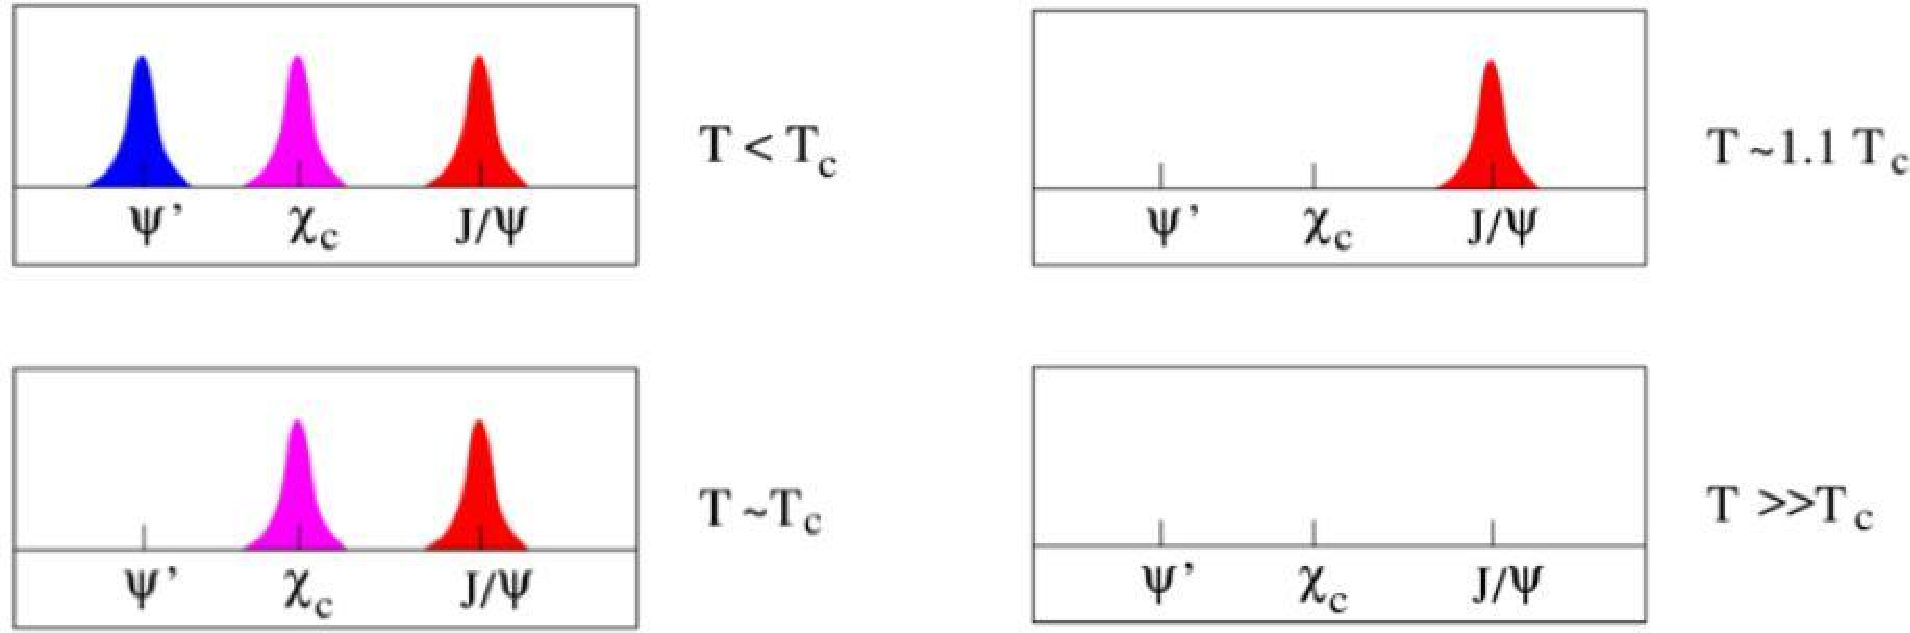
\includegraphics[width=\hugefigwidth]{chap_QuarkoniaSurvey_figures/Quarkonia_SATZ2}
  \caption[QuarkoniaAtTc]{Charmonium spectra at different temperatures \cite{SATZ2}.}
   \label{fig:QuarkoniaAtTc}
\end{figure}



LQCD can give accurate estimates of the quarkonium binding potential
as a function of the system temperature and the inter$-$quark separation
r in the relativistic limit. Such calculations allow them to predict the dissociation
temperatures T$_d$ of the quarkonium states. Table \ref{tab:quarkoniaproperties} summarizes
the results obtained by using the full internal energy (including the entropy
term) \cite{SATZ,Frithjof}. An illustration of the situation for the charmonium dissociation
temperatures is displayed in Figure \ref{fig:QuarkoniaAtTc}. A ``sequential melting'' pattern of the
various charmonium states with their binding energy is observed, the ground
state disappearing the last. Recent LQCD calculations support the late dissociation
of J/$\psi$($\Upsilon$) at about T$_d$/T$_c$ = 1.5(3.2) \cite{Matthias} in agreement with LQCD
spectral analysis of the hadron correlation functions \cite{Jakovac}.

\begin{table}[bht]
\caption[QuarkoniaProperties]{Dissociation temperatures of the quarkonium resonances from
LQCD. Where E$_b$ stands for the binding energy \cite{SATZ, Rev_PartPhysics, Frithjof}.}
\label{tab:quarkoniaproperties}
\begin{tabular}{lllllllll}
\hline
               &J/$\psi$(1S)  &$\chi_c$(1P)  &$\psi^{1}$(2S)  &$\Upsilon(1S)$  &$\chi_b$(1P)  &$\Upsilon$(2S)  &$\chi_b$(2P)  &$\Upsilon$(3S) \\
\hline
M[GeV]             &3.10          &3.41          &3.69           &9.46            &9.86           &10.02          &10.23         &10.36  \\              
E$_b$[GeV]         &0.64          &0.20          &0.05           &1.10            &0.67           &0.54           &0.31          &0.20   \\
$\frac{T_d}{T_c}$  &2.1           &1.16          &1.12            &$\geq$4.0      &1.76           &1.60           &1.19          &1.17   \\
\hline
\end{tabular}
\end{table}


\section{Experimental Status of Quarkonia Suppression}

\subsection{J/$\psi$ anomalous suppression at SPS}
A first J/$\psi$  suppression was observed and reported by the NA38 experiment
\cite{NA38}, which was performed with oxygen-uranium collisions of incident energy
200 GeV per nucleon. Figure \ref{fig:JPsiAtSPSNA38} shows the measured J/$\psi$  yield normalized
to the number of dimuons in mass range 2.7$-$3.5 GeV/c$^2$ as a function of transverse
energy (E$_T$ ) corresponded to centrality. A similar pattern was observed
later in sulphur-uranium collisions \cite{NA50}. Increasing centrality, the nuclear matter
is more and more compressed, at some point a volume of deconfined matter
forms with free color charges. Charmonium binding potential is screened and
the bound state is dissolved and then the measured J/$\psi$  production decreases
with respect to the reference. Because the ratio would be expected to remain
constant with respect to the centrality if charmonium is not suppressed.
However, another trial of explanation is possible without deconfinement
for the charmonium dissociation. It can be happened in the interactions with
nucleons. As pointed out in \cite{Khar_Carlos} the observed suppression is able to be presented
by the breakup of charmonium caused by scattering off nucleons, where
the matter is confined. The experiment of smaller system such as proton$-$nucleus
or deuterium$-$nucleus collisions was designed to examine this effect,
namely nuclear absorption. Indeed the effect of nuclear absorption was measured,
absorption cross section as $\sigma_{\mbox{abs}}$ = 7.3$\pm$0.6 mb \cite{Khar_Carlos}. 
The NA50 experiment compared the charmonium production to the Drell-Yan (q$\overline{q}\rightarrow l^+l^-$) 
process, since the compete dimuon continuum in the J/$\psi$  mass range can not be predicted
from theory \cite{NA51}. Figure \ref{fig:JPsiAtSPS} illustrates the ratio of J/$\psi$  and Drell$-$Yan
process as a function of L, the length of traversed nuclear matter, which can
be obtained from Glauber model calculation \cite{Khar_Carlos,NA51_2}. Thus the line shows the
amount of suppression due to nuclear absorption, that can not be related to
the dissociation from deconfinement. A clear deviation from this line can be
observed for L $>$ 7.5 fm. This suppression is called the anomalous suppression.

To determine the energy density necessary to melt charmonium, measurements on smaller 
systems have been performed. Although the maximum achievable energy density is smaller 
than in collisions of larger nuclei, smaller systems enable a higher resolution centrality 
scan. The results are shown in Figure \ref{fig:JPsiAtSPSNA50} (left) \cite{Scomparin}. 
The J/$\psi$/Drell-Yan production is plotted as a function of
the number of participants in the collision, where the data is normalized to cold
matter effects. A suppression exceeding the nuclear suppression is seen starting from 80 
participants on. In Figure \ref{fig:JPsiAtSPSNA50} (right) the data is compared to the
results of the NA50 experiments from lead-lead collisions of the same energy of
158 GeV per nucleon. For peripheral collisions the ratio of measured/expected
J/$\psi$ yield is as expected, close to one, any observed dissociation is attributed
to cold nuclear effects. For more central collisions a clear deviation from the
expected behavior is observed, with good agreement between the In$-$In and the
Pb$-$Pb data
The measurement of $\psi^{'}$ has been performed as shown in Figure \ref{fig:PsiAtSPSNA50NA60}. All
the measurements suffer from the significantly lower statistics accumulated
for the $\psi^{'}$, because it is not only due to the lower production cross section,
but dominantly due to the lower branching into dileptons ($\sigma_{\psi^{'}} \rightarrow l^{+}l^{-}= 0.73 \%$
compared to $\sigma_{J/\psi} \rightarrow l^{+}l^{-}= 5.9 \%$ ).
Figure \ref{fig:PsiAtSPSNA50NA60} presents the similar suppression of $\psi^{'}$ is observed compared to
the J/$\psi$ only the onset of the anomalous suppression is already at L = 4fm
and thus happens at a lower energy density.

\subsection{J/$\psi$ and $\Upsilon(nS)$ suppression at RHIC}
At RHIC J/$\psi$ yield in AA collisions is compared with scaled yield in p+p collisions. 
It gives a new varibale known as Nuclear Modification Factor or R$_{AA}$.
\begin{eqnarray}
R_{AA} &= \frac{1}{N_{Coll}} \frac{\frac{d^{2}N^{J/\Psi}_{AA}}{dy dp_{T}}}{ \frac{d^{2}N^{J/\Psi}_{pp}}{dy dp_{T}}} \\
\end{eqnarray}

\subsubsection{J/$\psi$ suppression at PHENIX}
Figure \ref{fig:JPsiAtPHENIX1} shows the suppression pattern observed by PHENIX in Au$-$
Au and Cu$-$Cu collisions. The suppression of J/$\psi$  is observed in the more
central collisions. Since cold nuclear matter effects are not subtracted here the
observed suppression can not be attributed to the dissociation of quarkonia in
the deconfined medium alone. Figure \ref{fig:JPsiAtPHENIX2} presents the ratio of R$_{AA}$ and cold
nuclear matter effects (CNM) \cite{Phenix1}. For the comparison to previous results, the
J/$\psi$  data taken by NA50 and NA60 are included. The data agree quite well
between SPS and RHIC in the lower energy densities, while the suppression
observed at RHIC clearly exceeds the maximal suppression measured at SPS
of R$_{AA}$/CNM = 60 $\%$ in the higher energy densities

In particular, PHENIX measured R$_{AA}$ at different rapidity region. 
Figure \ref{fig:JPsiAtPHENIX2} illustrates J/$\psi$  R$_{AA}$ in four different centrality bins 
as a function of rapidity. While R$_{AA}$ is almost constant for peripheral collisions 
(centrality bins 40-60 $\%$ and 60-92 $\%$), the central collisions show a clear 
difference between forward and mid rapidity. The suppression of J/$\psi$  production is 
significantly lower in forward/backward direction compared to the observed suppression
at mid rapidity. This phenomenon could so far not be explained by current
quarkonia production and suppression models.


\begin{figure}
  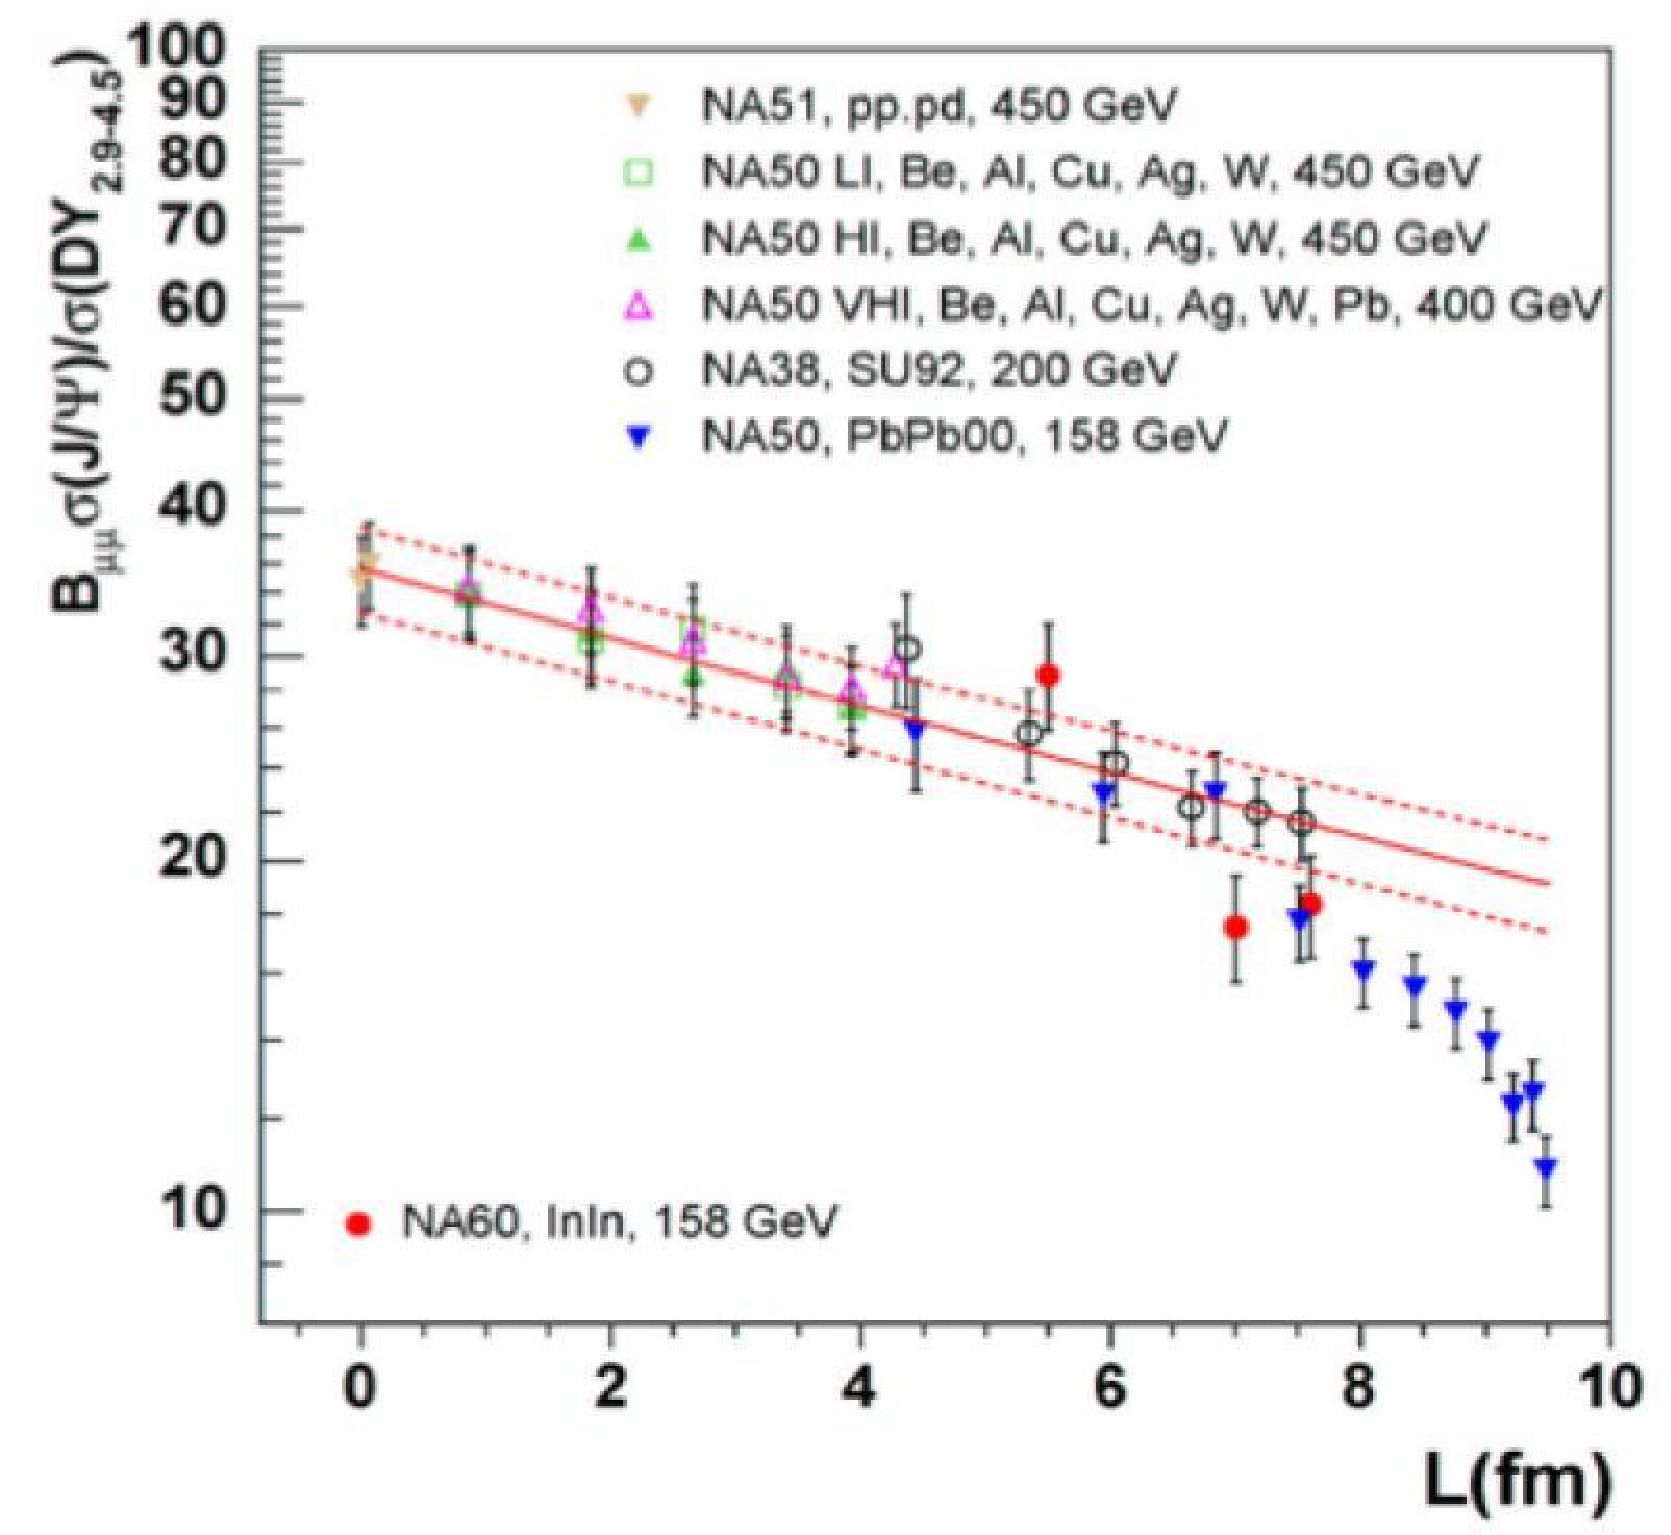
\includegraphics[width=\largefigwidth]{chap_QuarkoniaSurvey_figures/SPSNA51_27}
  \caption[JPsiAtSPSCrossSection]{J/$\psi$ over Drell$-$Yan production cross$-$section ratio as a function
of the length traversed by the charmonium in nuclear matter (L) for various colliding systems \cite{Pillot}.}
   \label{fig:JPsiAtSPS}
\end{figure}


\begin{figure}
  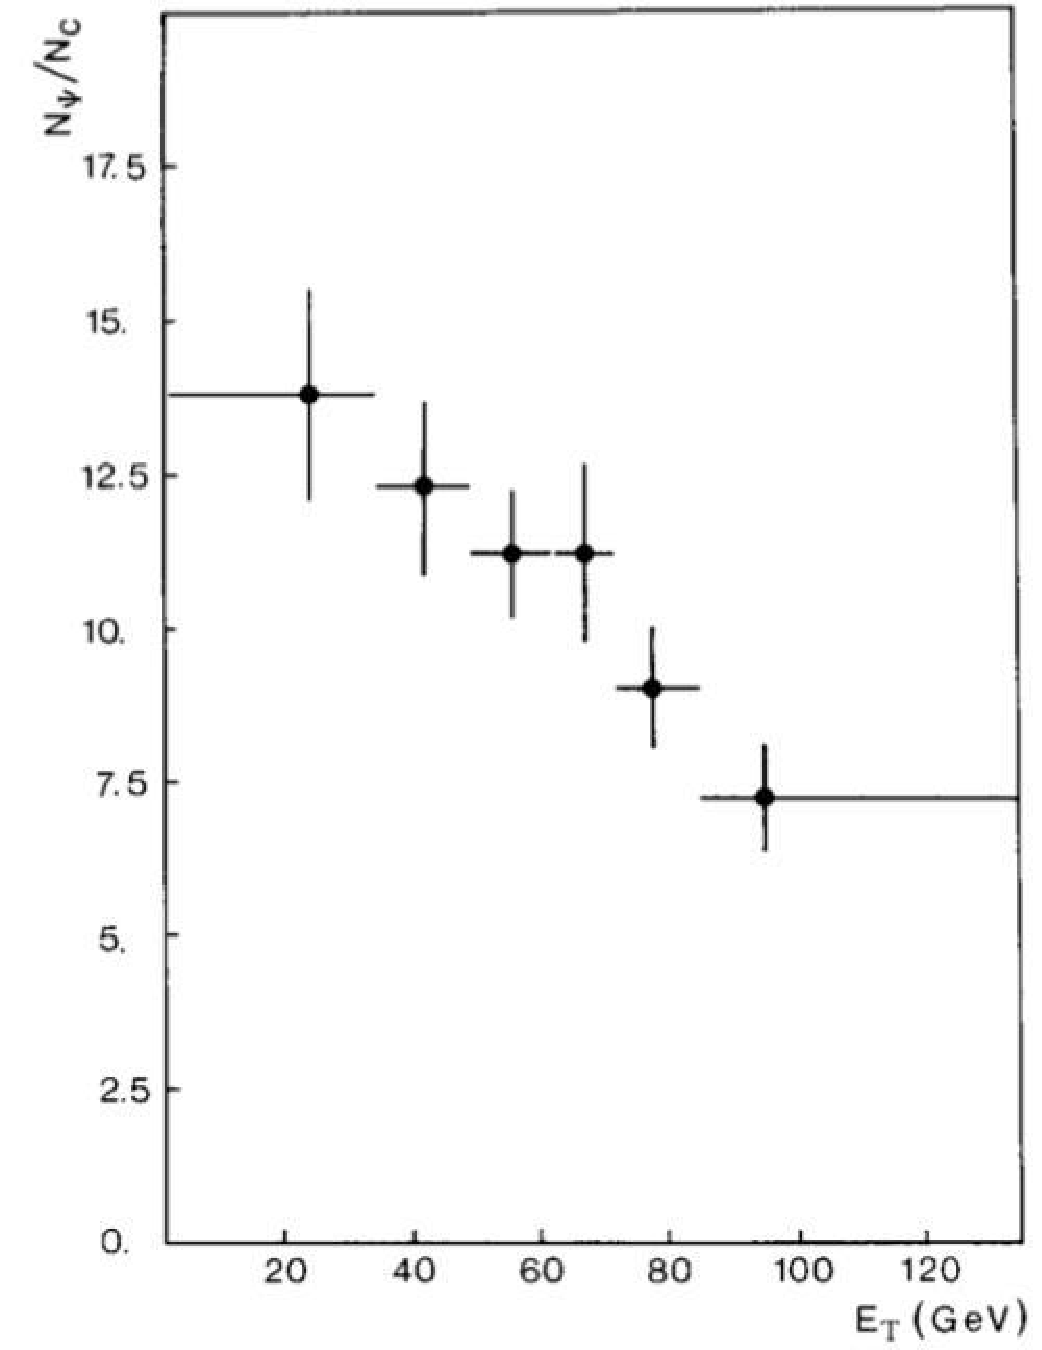
\includegraphics[width=\largefigwidth]{chap_QuarkoniaSurvey_figures/SPS_216}
  \caption[JPsiNA38]{The ratio of produced J/$\psi$  and dimuons as a function of the transverse energy as measured by NA38 \cite{NA38}.}
   \label{fig:JPsiAtSPSNA38}
\end{figure}



\begin{figure}
  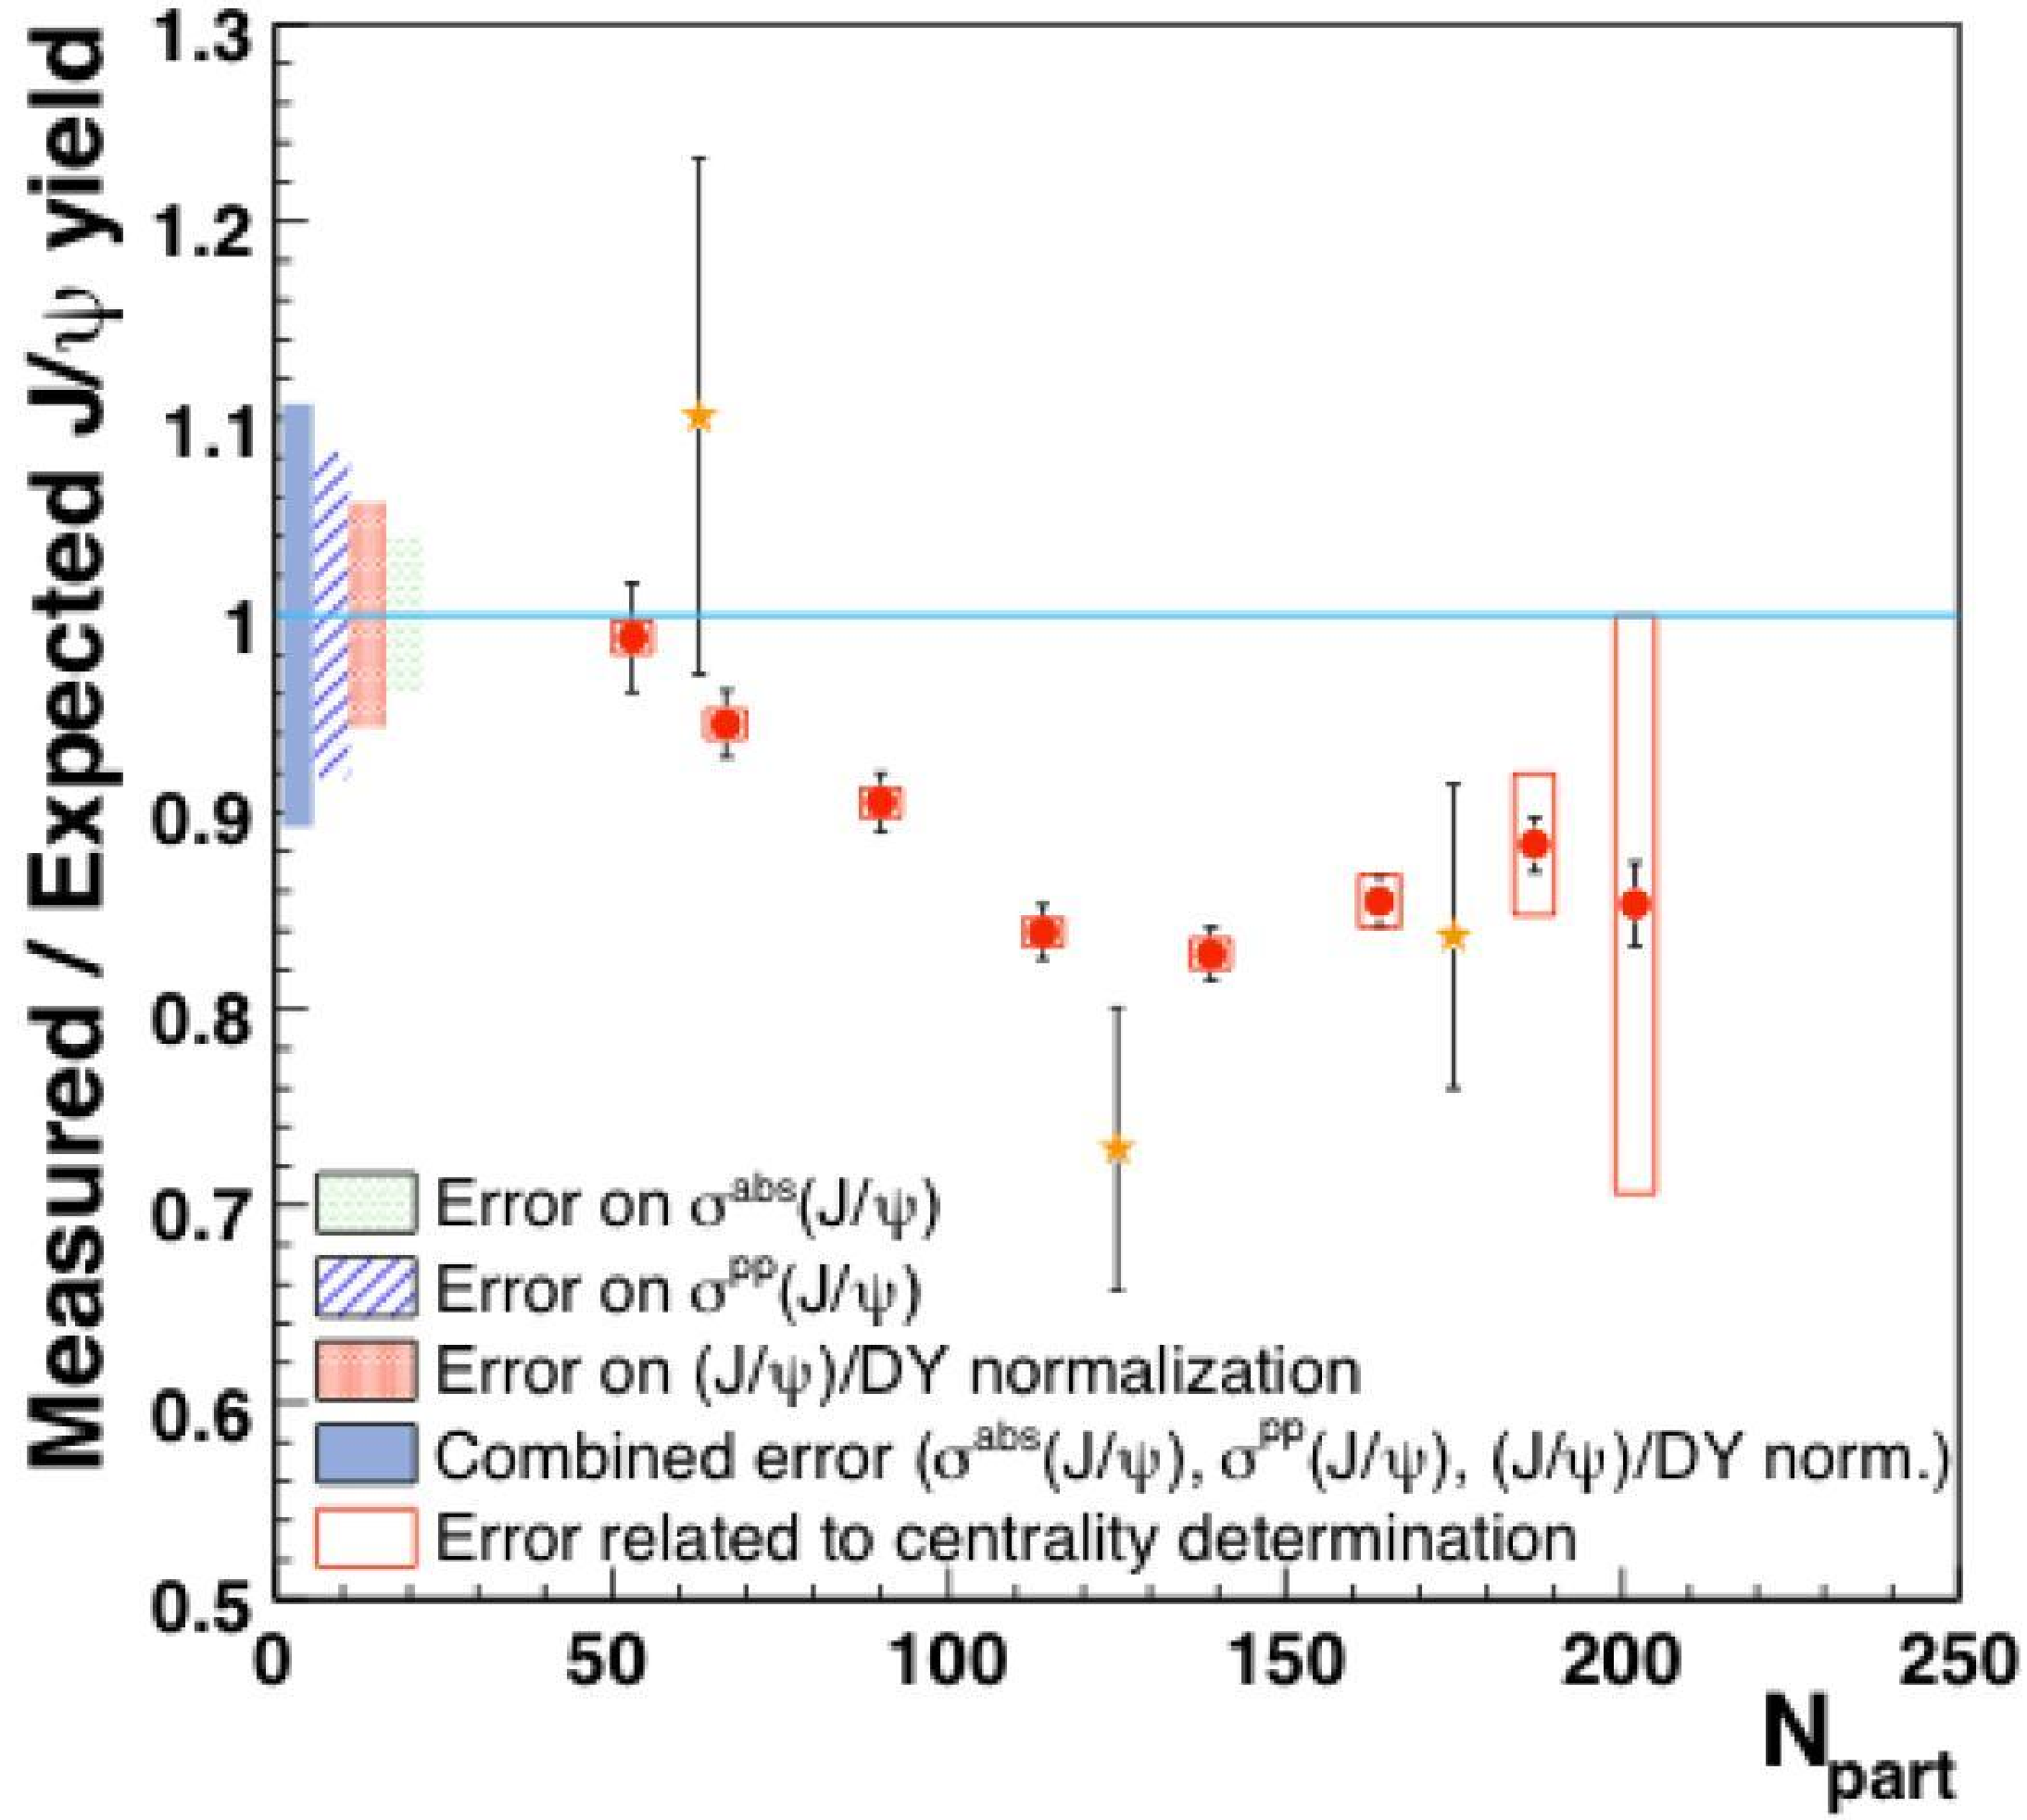
\includegraphics[width=\smallfigwidth]{chap_QuarkoniaSurvey_figures/SPS_217_1}
  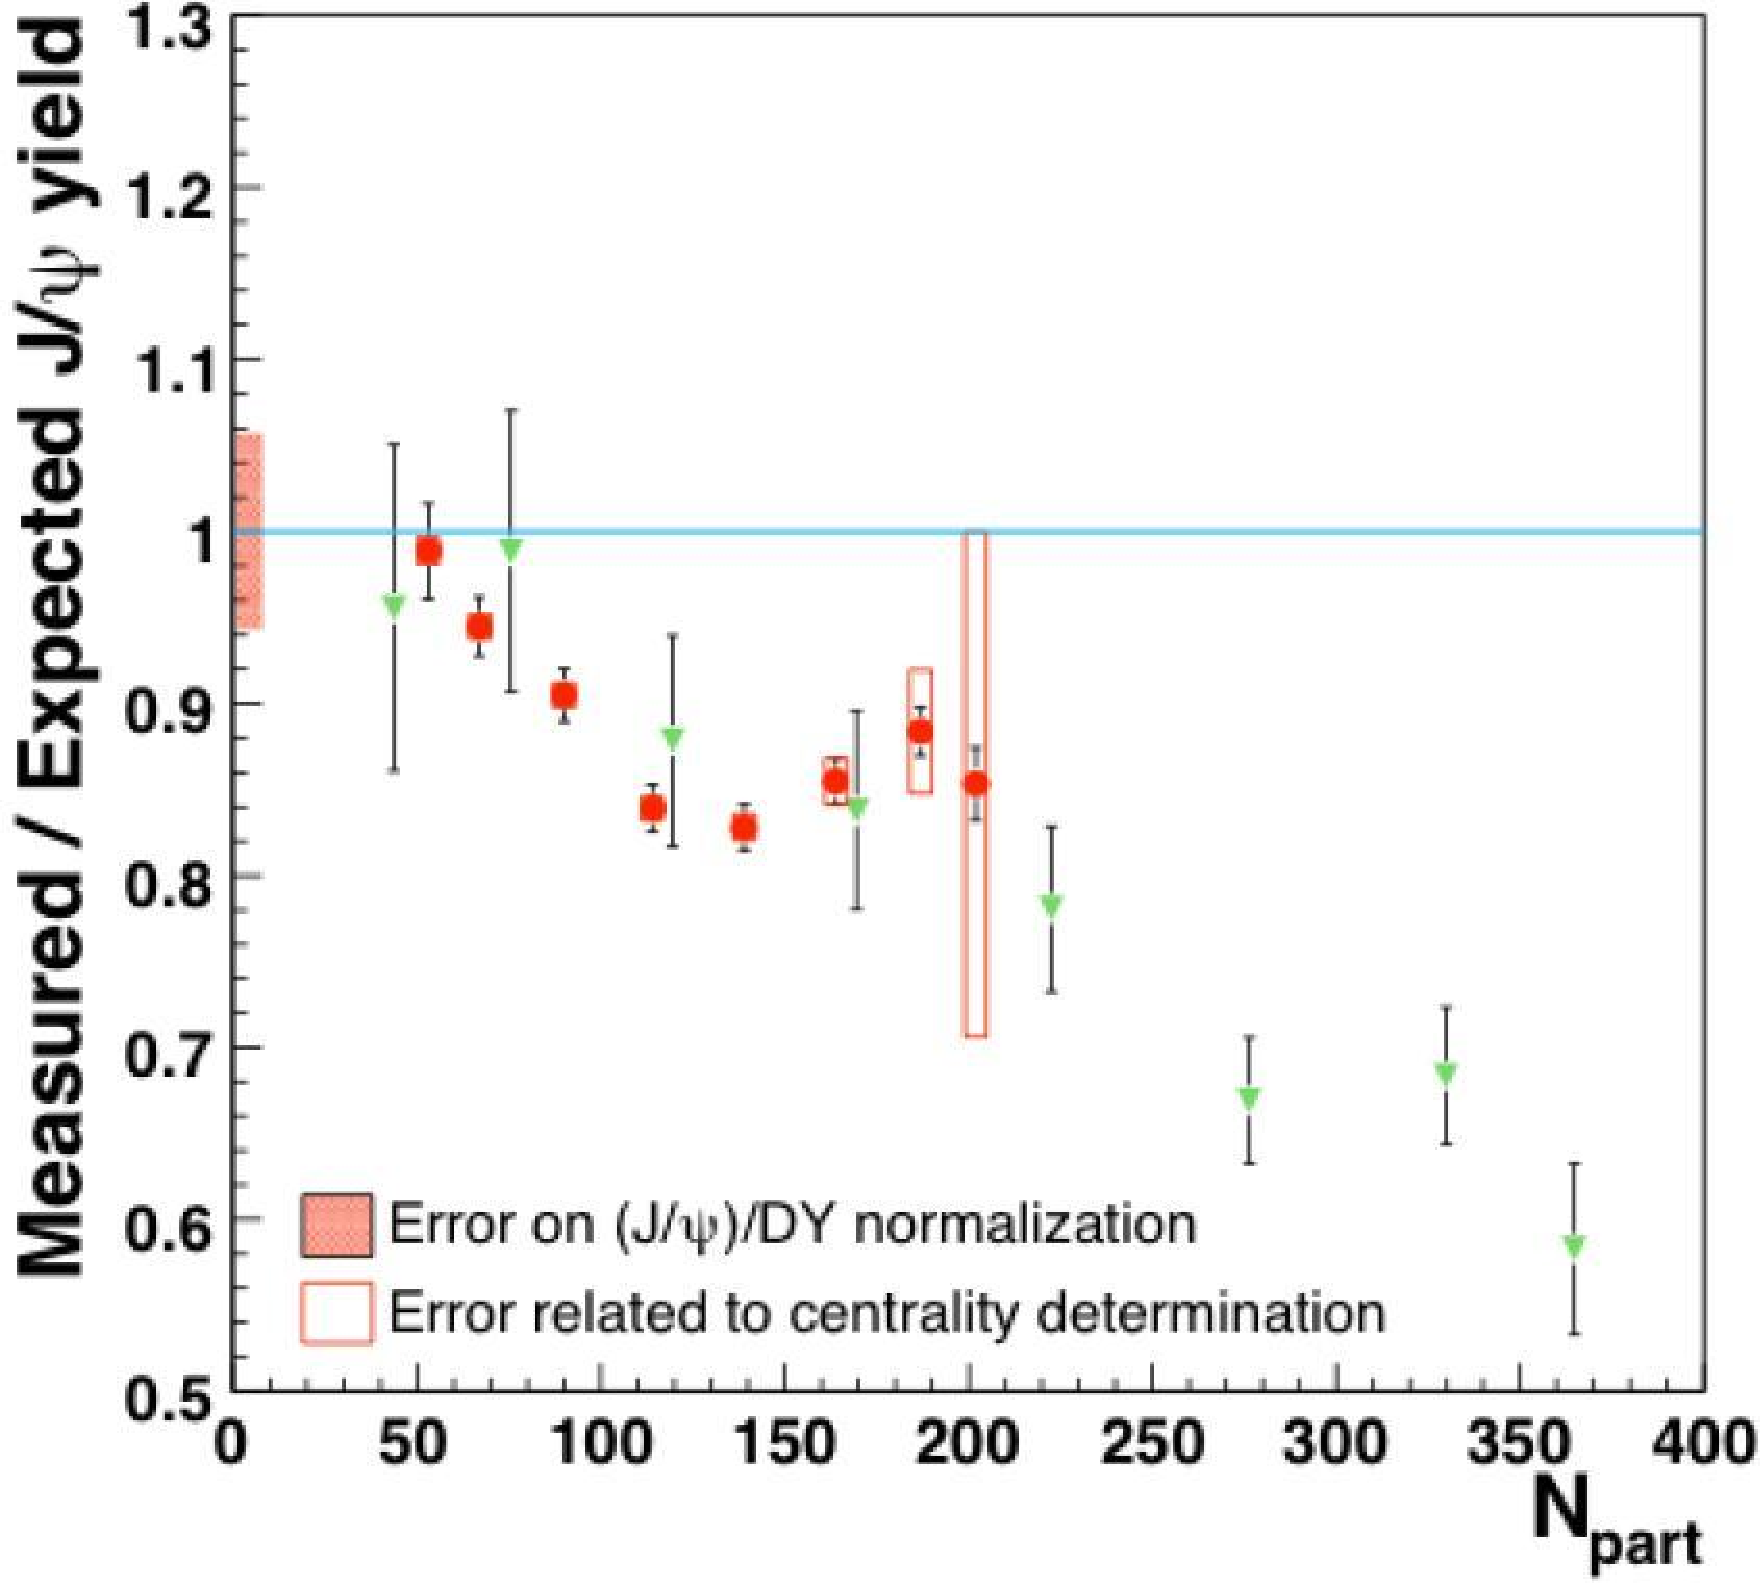
\includegraphics[width=\smallfigwidth]{chap_QuarkoniaSurvey_figures/SPS_217_2}
  \caption[JPsiNA50]{The centrality dependence of the J/$\psi$  suppression for In$-$In collisions at 158 GeV per nucleon measured by NA60 (left). 
    A comparison between the NA60 In$-$In and the NA50 Pb-Pb data (right).}
  \label{fig:JPsiAtSPSNA50}
\end{figure}




\begin{figure}
  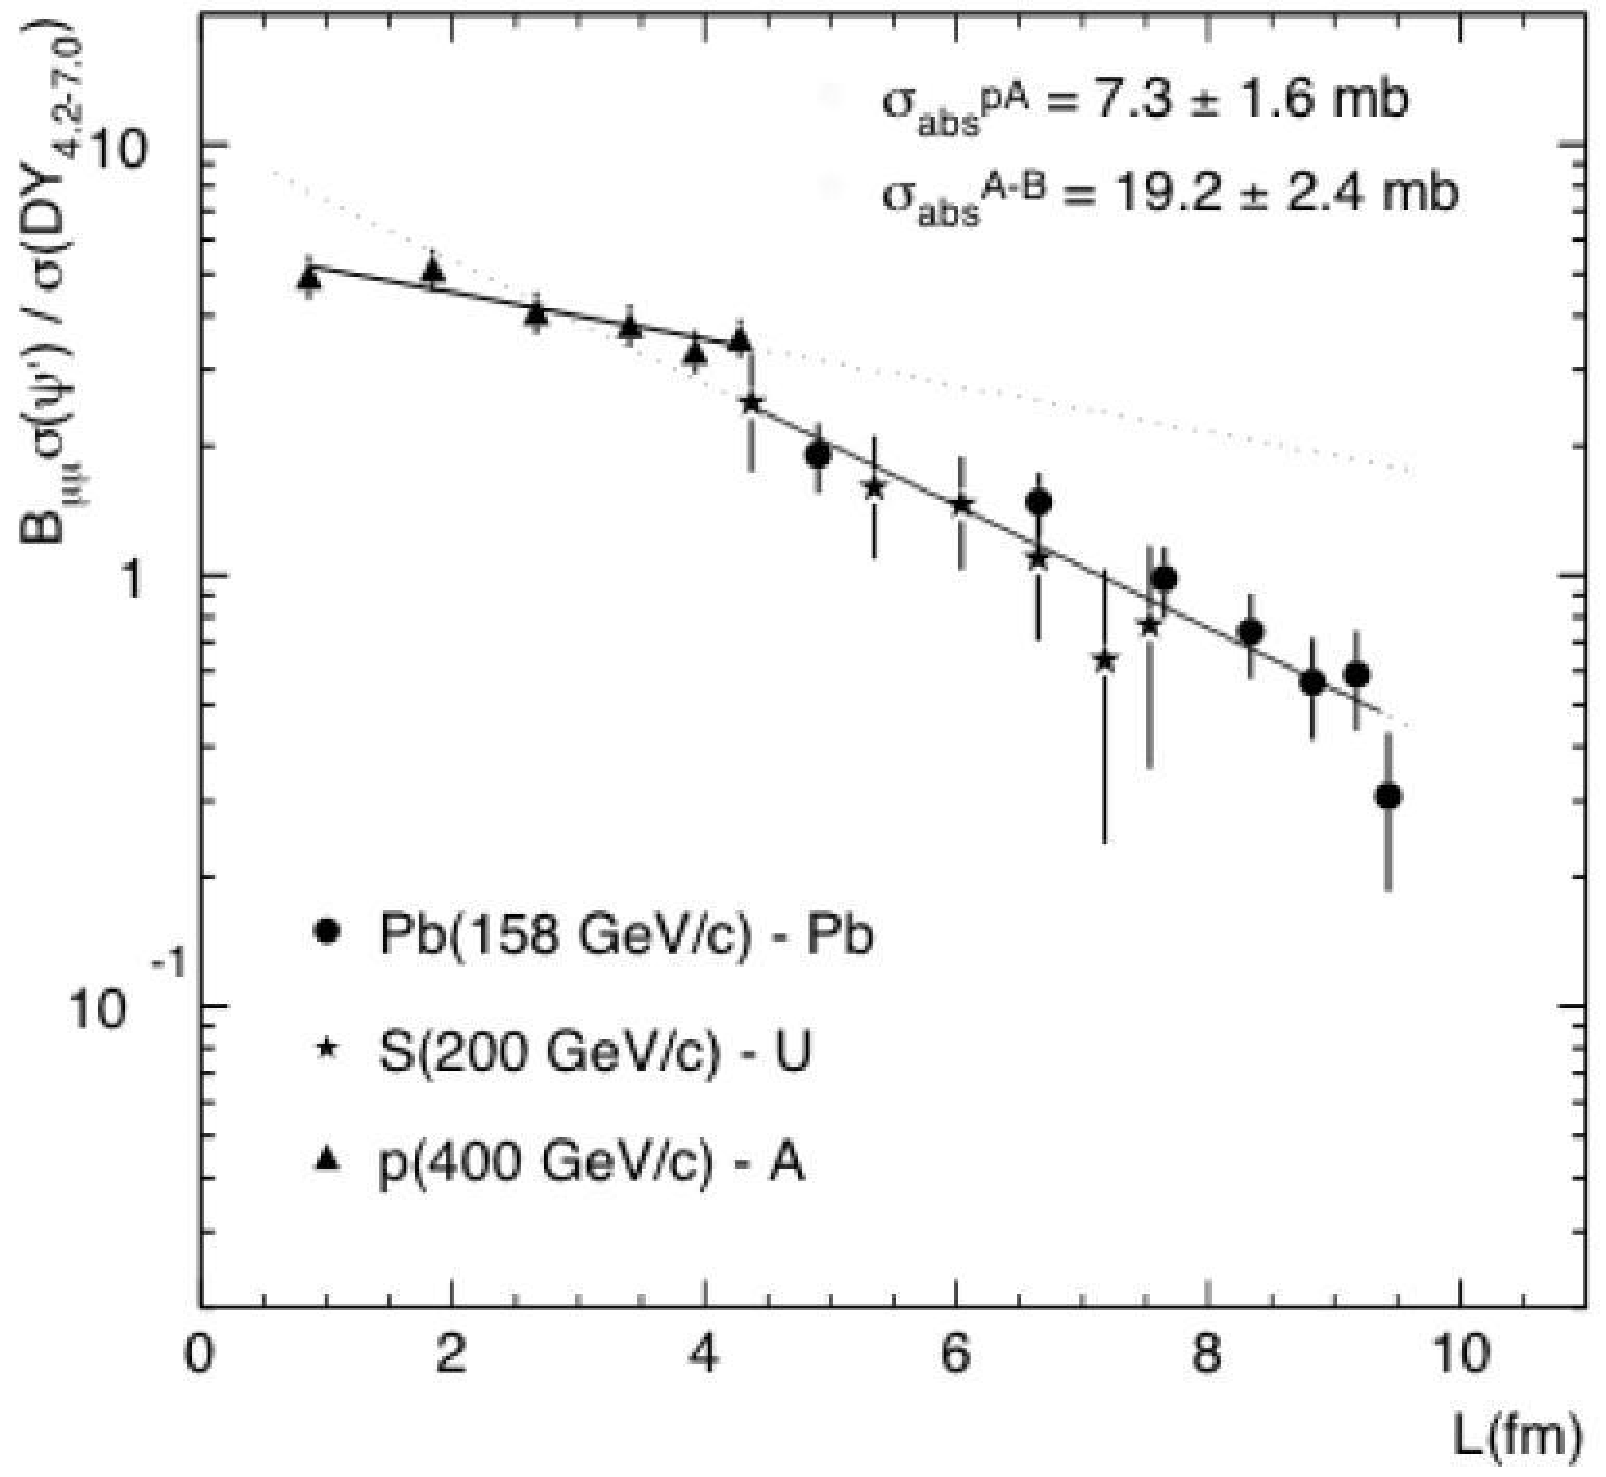
\includegraphics[width=\smallfigwidth]{chap_QuarkoniaSurvey_figures/SPS_Psi_218_1}
  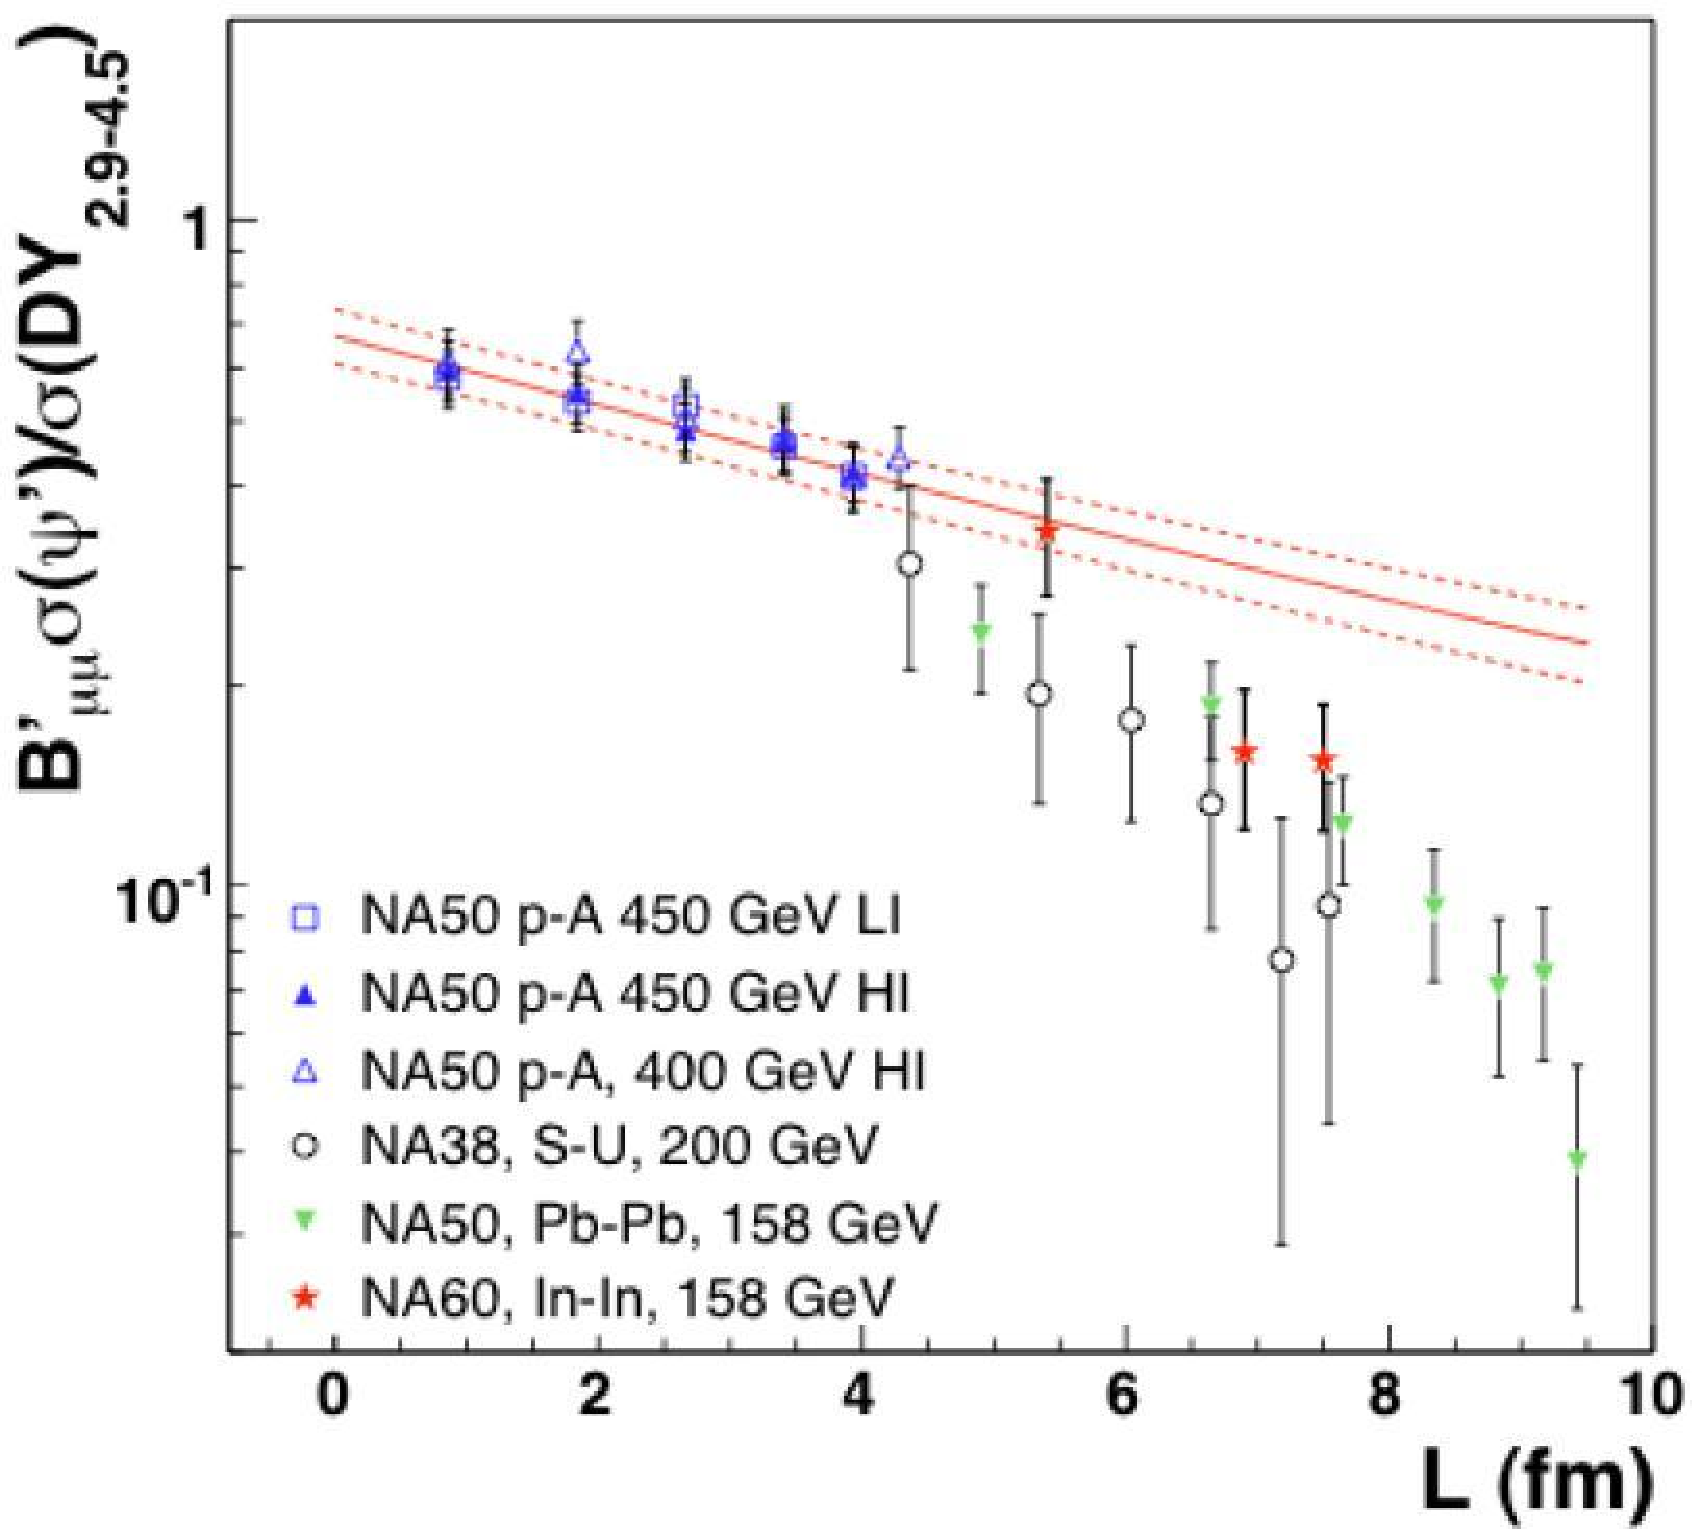
\includegraphics[width=\smallfigwidth]{chap_QuarkoniaSurvey_figures/SPS_Psi_218_2}
  \caption[PsiNA50NA60]{The ratio between cross section of $\psi^{'}$ times the branching into
    muons (B$_{\mu^{+}\mu^{-}}$) and the cross section of Drell$-$Yan reference process as measured
    by the NA50 and NA60 at various energies and in different collisional systems}
  \label{fig:PsiAtSPSNA50NA60}
\end{figure}


\begin{figure}
  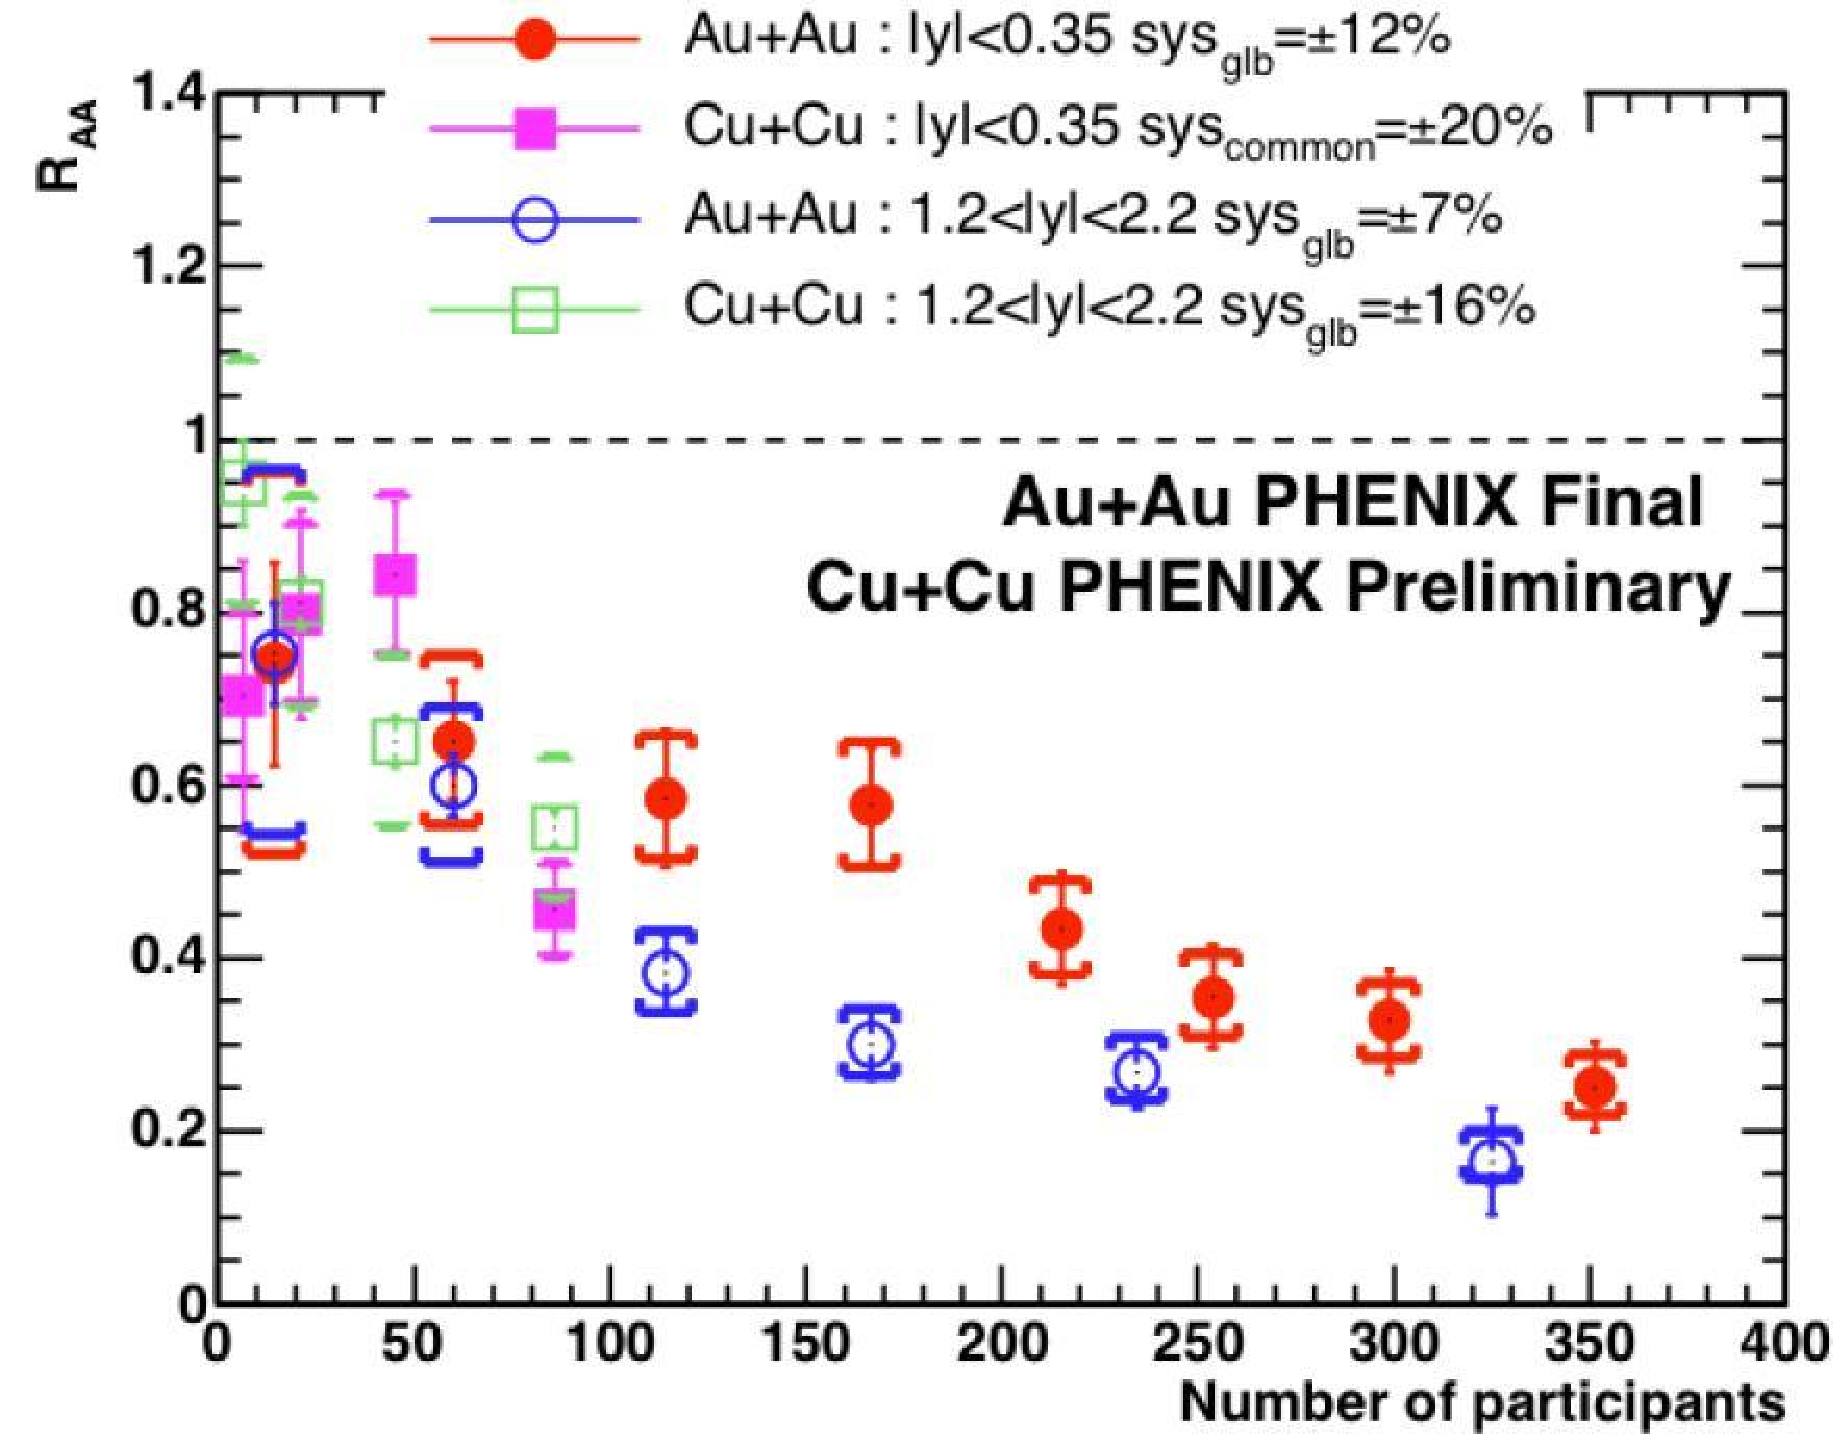
\includegraphics[width=\hugefigwidth]{chap_QuarkoniaSurvey_figures/RHIC_JPsi_219_1}
  \caption[JPsiRHICPhenix]{R$_{AA}$ as a function of Npart measured by PHENIX in Au$-$Au (in circles) and Cu$-$Cu (in squares) \cite{Phenix2}.}
   \label{fig:JPsiAtPHENIX1}
\end{figure}


\begin{figure}
  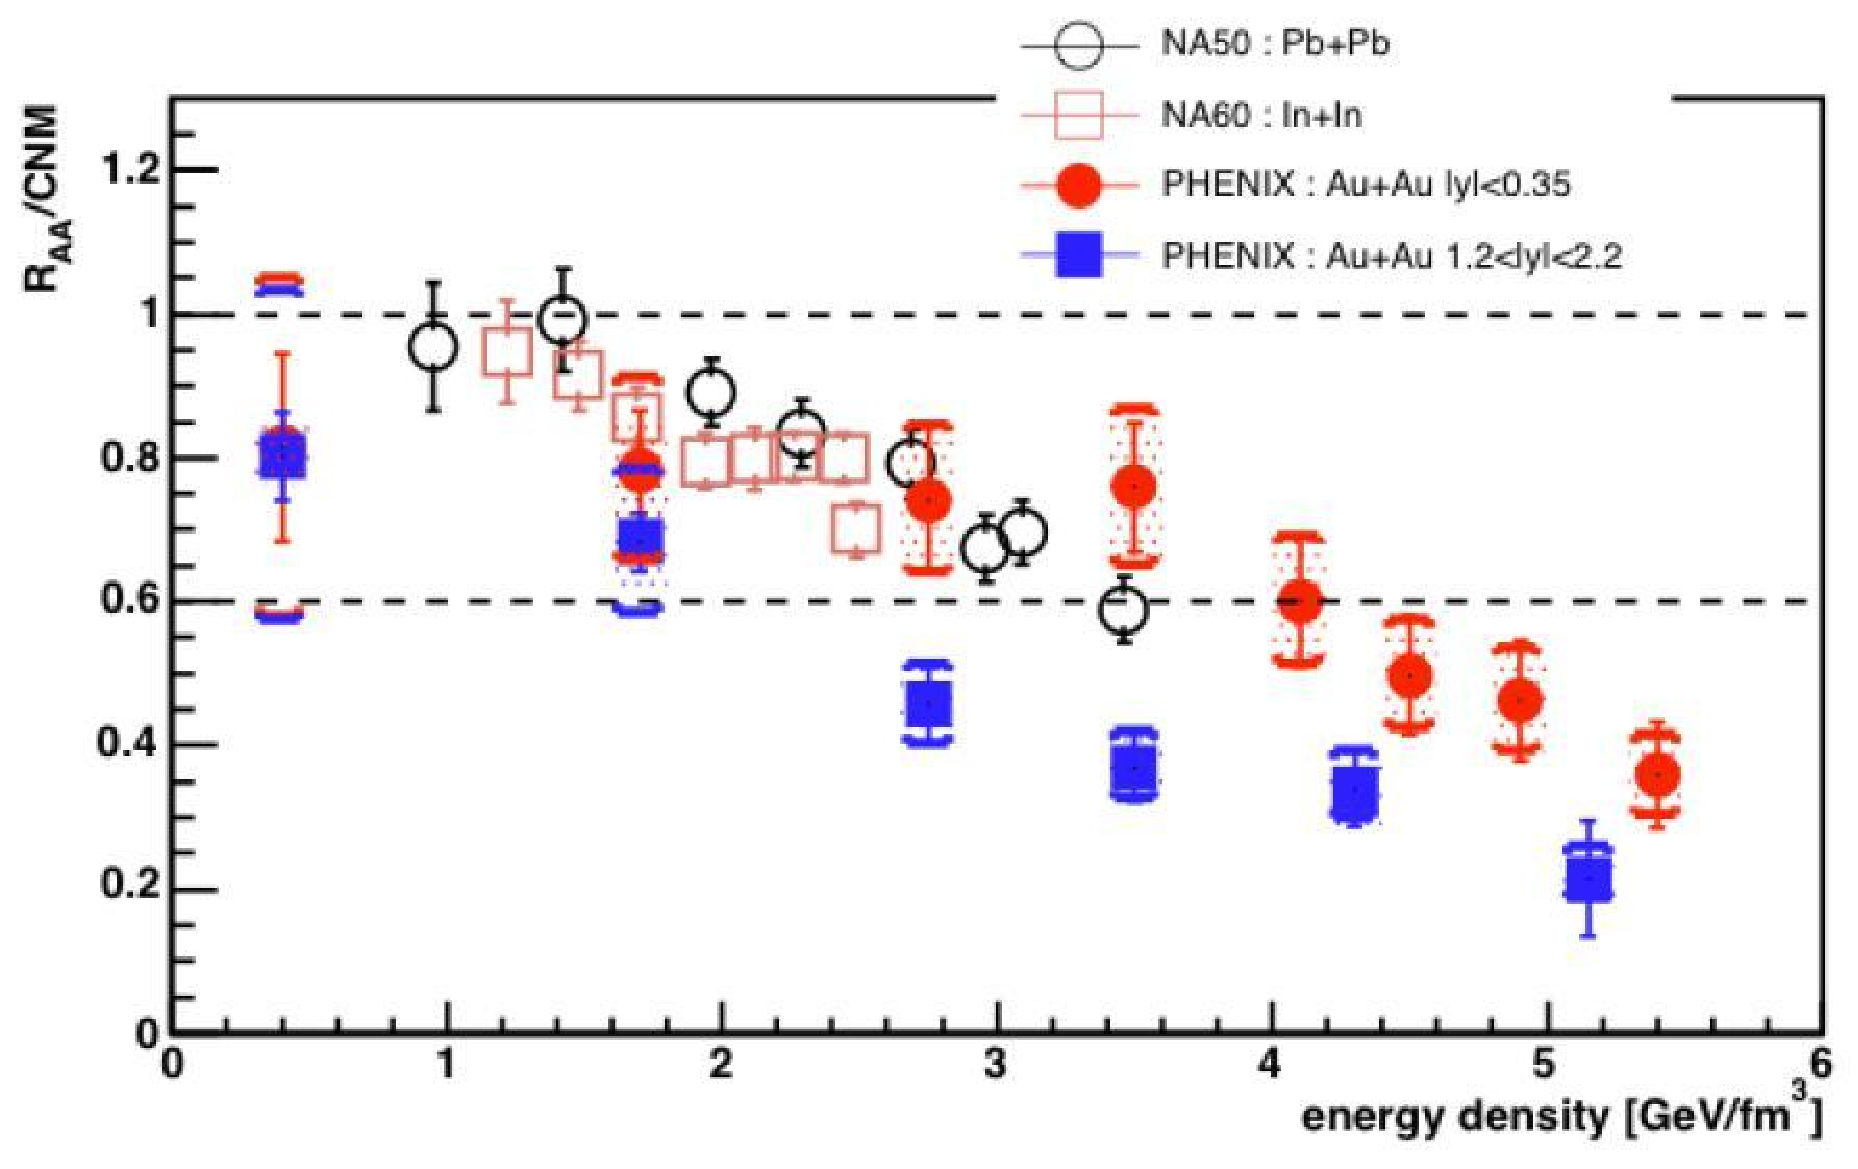
\includegraphics[width=\hugefigwidth]{chap_QuarkoniaSurvey_figures/RHIC_JPsi_219_2}
  \caption[JPsiRHICPhenix2]{R$_{AA}$/CNM as a function of the Bjorken estimate of the energy
     density. The RHIC data ($\sqrt{s_{NN}}$ = 200 GeV) is compared to SPS (17.3 GeV)
     measurements performed by NA50 and NA60 [70]. PHENIX estimates the cold nuclear matter 
     effects from measurements on d$-$Au, while the NA50 and NA60 rely on theoretical calculations.}
   \label{fig:JPsiAtPHENIX2}
\end{figure}

%\subsubsection{J/$\psi$ suppression at STAR}

\subsubsection{$\Upsilon(nS)$ suppression at RHIC}
STAR experiment at RHIC measure high p$_T$ J/$\psi$ and $\Upsilon$ states. 
Due to small production cross-section of b quark at 200 GeV, total yield 
of $\Upsilon$ is very small. STAR measure $\ee$ pairs ar mid rapidity $(|y| \leq 0.5)$. The unlike sign invariant
mass distribution, after subtracting like sign background is shown in Figure~\ref{fig:YinSTAR}:left. The measured yield
contain $\Upsilon$ signal as well as background from Drell$-$Yan and semileptonic decay of open beauty mesons.
The line-shape of the $\Upsilon$(1S+2S+3S) was parameterized with three crystal ball functions representing the successive states.
Different $\Upsilon$ states can not be seperated because of poor mass resolution as shown in Figure~\ref{fig:YinSTAR}:left.  
Measured $\Upsilon$ yield is devided in to three centrality bins: 0 $\%$ to 10$\%$, 10$\%$ to 30$\%$, and 30$\%$ to 60$\%$. 
R$_{AA}$ for the three centrality bins is shown in Figure~\ref{fig:YinSTAR}:right.
The results are compared to a model \cite{StrickLand} which incorporates lattice-based QCD calculations with a hydrodynamic
model of expansion and cooling. 
%[2] M. Strickland, D. Bazow arXiv:1112.2761v4,

\begin{figure}
  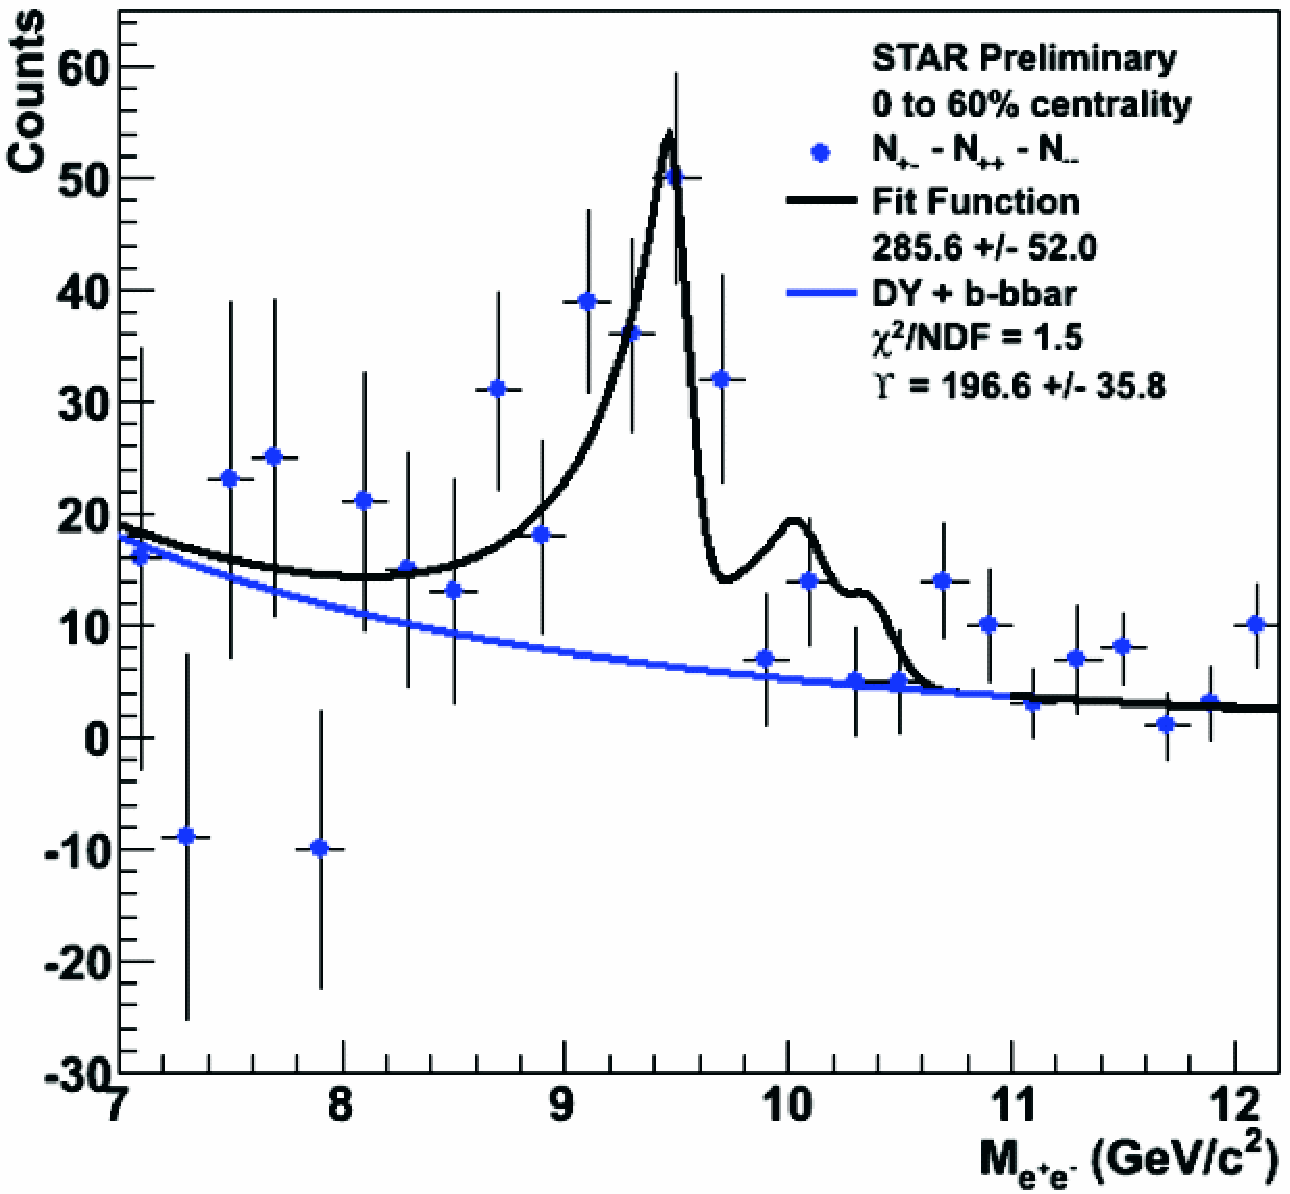
\includegraphics[width=\smallfigwidth]{chap_QuarkoniaSurvey_figures/YStar2011_InvMass}
  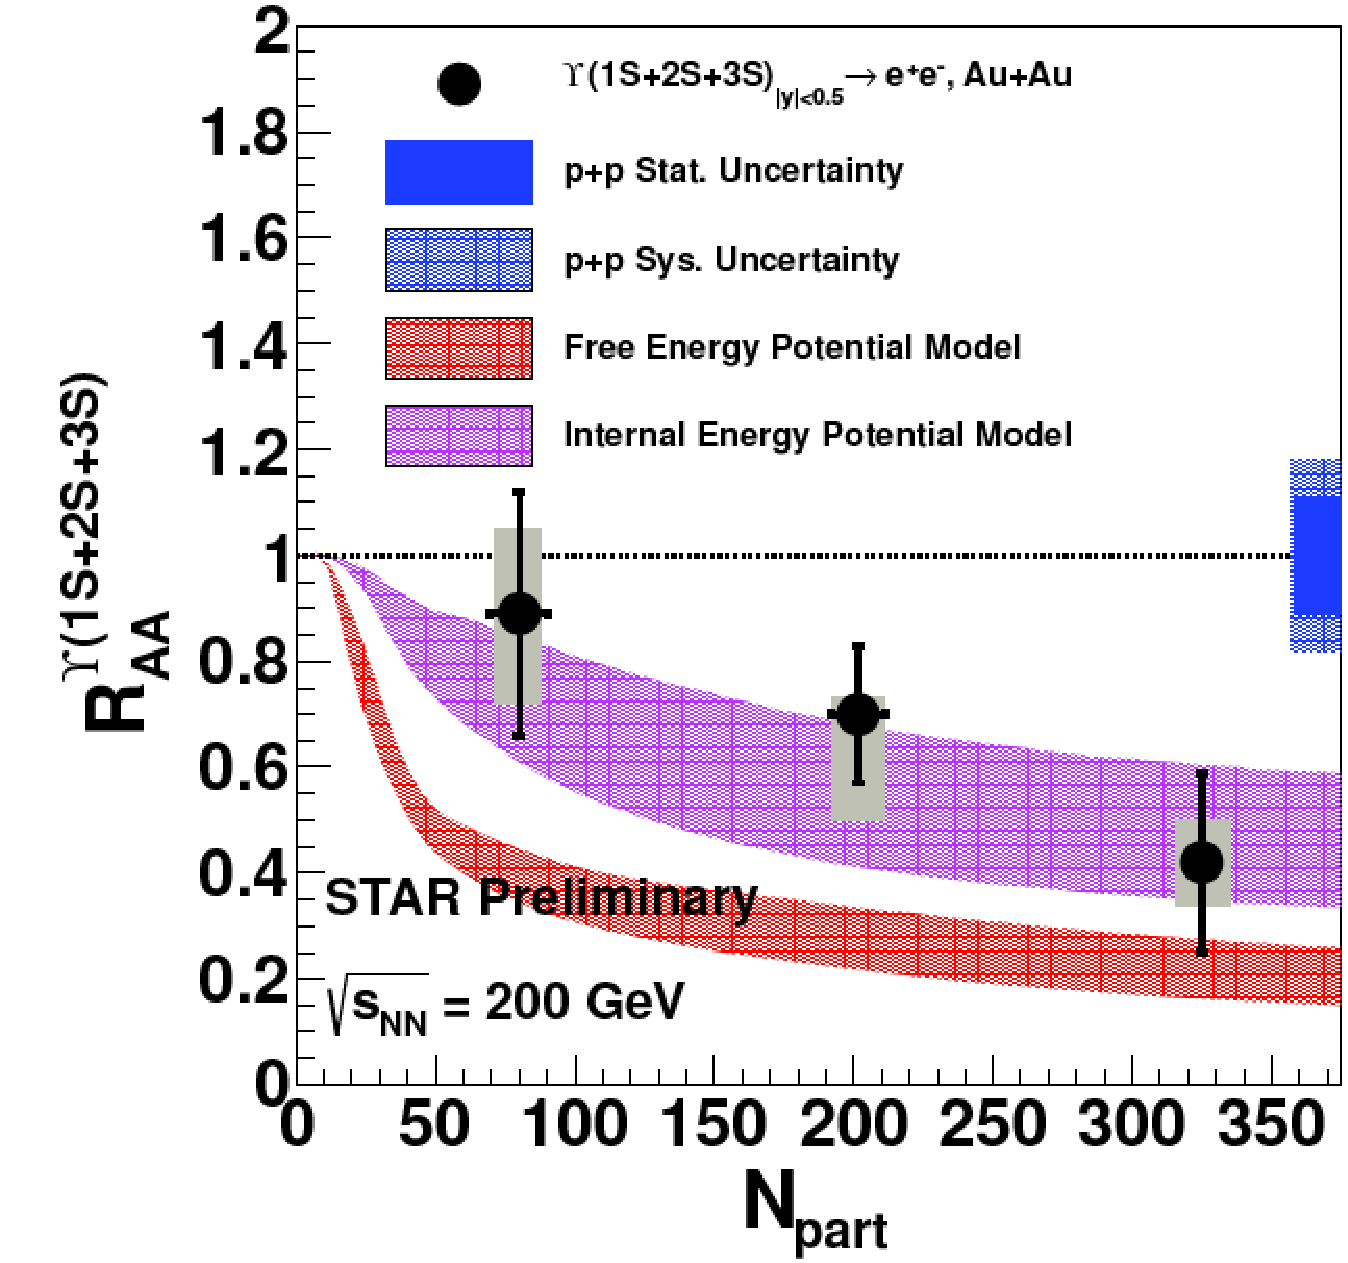
\includegraphics[width=\smallfigwidth]{chap_QuarkoniaSurvey_figures/YStar2011}
  \caption[]{left:$\ee$ pairs as measured in STAR detector at RHIC in 0$\%$-60$\%$ centrality class. The blue curve is the combination of Drell$-$Yan and b $\overline {b}$ 
    background. The black curve includes the Upsilon signal also. right: R$_{AA}$for 2010 Au+Au compared to 2009 p+p. The magenta and orange curves are theoretical 
    predictions using a combination of lattice-based QCD and hydrodynamical expansion and cooling \cite{Star12}.}
  \label{fig:YinSTAR}
\end{figure}




\begin{figure}
  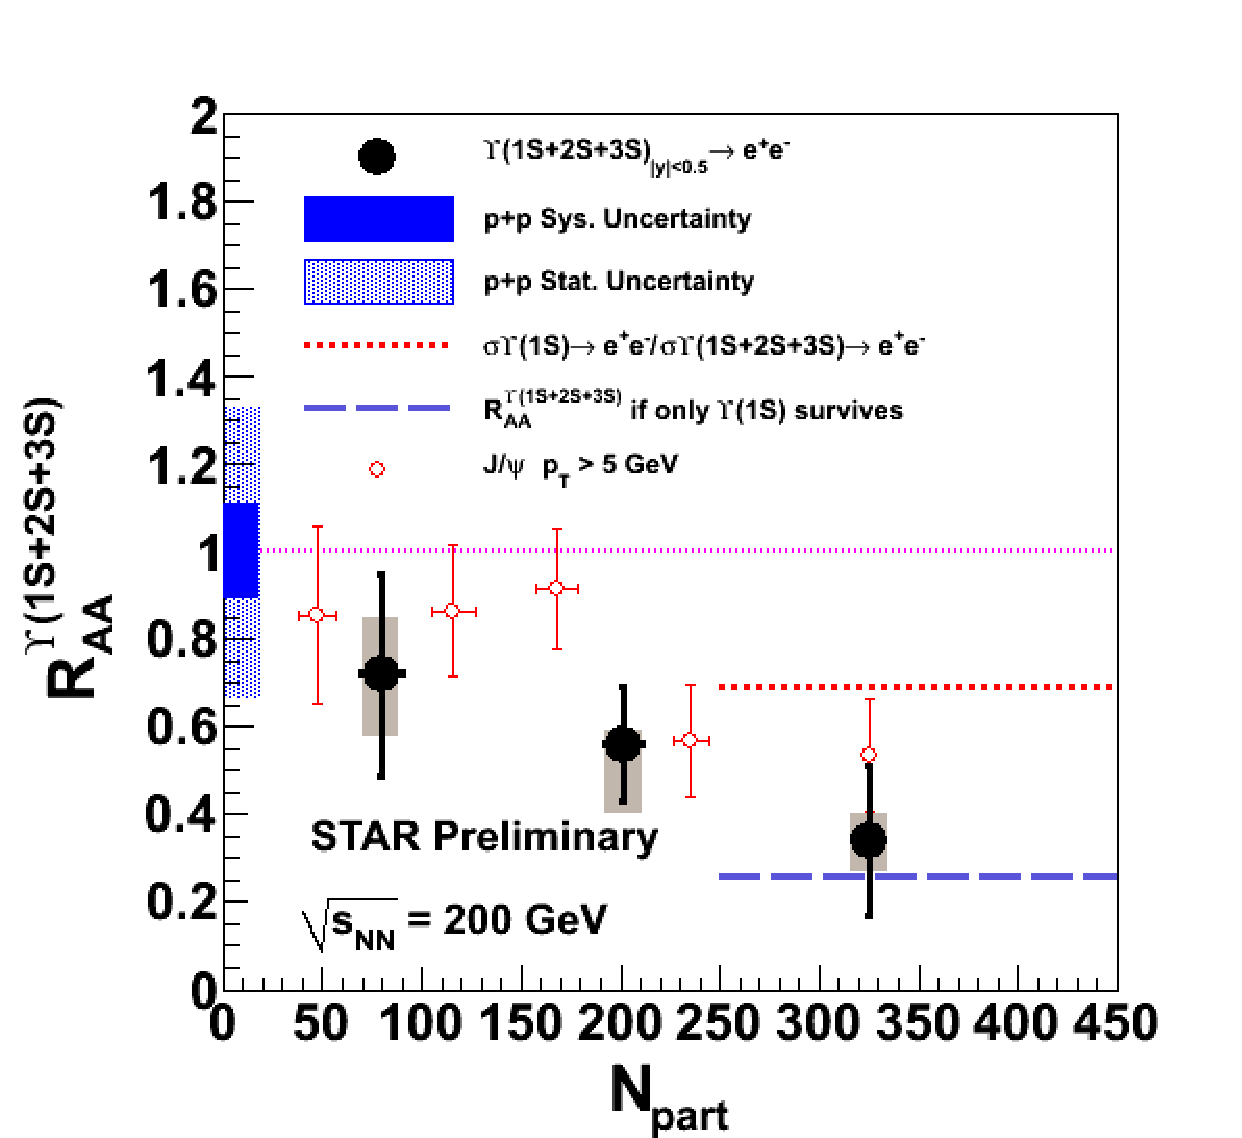
\includegraphics[width=\mediumfigwidth]{chap_QuarkoniaSurvey_figures/YStar2011_JPsiCompare}
  \caption[]{R$_{AA}$ for $\Upsilon(1S+2S+3S)$  versus centrality measured by STAR experiment at RHIC. The solid black points are the $\Upsilon$ R$_{AA}$. 
    The red open points are the high p$_T$ J/$\psi$ results from STAR. $\Upsilon$ R$_{AA}$ is compariable to J/$\psi$ in most central collisions.\cite{Star11}}
  \label{fig:YinSTAR2}
\end{figure}

Figure \ref{fig:YinSTAR2} shows $\Upsilon\,R_{AA}$ compared with high p$_T$ J/$\psi$ measured by STAR. A clear trend versus centrality can be seen in this graph.
The red dotted line is the ratio of the total cross-section of $\Upsilon$(1S)/$\Upsilon$(1S+2S+3S). The purple dashed line is the ratio of only the direct 
$\Upsilon$(1S) cross-section over the total $\Upsilon$(1S+2S+3S) cross-section. $\Upsilon$ R$_{AA}$ is compariable to J/$\psi$ in most central collisions. 


  
\chapter{The Compact Muon Solenoid Experiment at The CERN Large Hadron Collider}
\label{chap:CmsExp}

\section{The \LHC}

The Large Hadron Collider (LHC) at CERN near Geneva is the world's newest and
most powerful tool for Particle Physics research. It is designed to collide proton beams with a
centre-of-mass energy of 14 TeV and an unprecedented luminosity of 10$^{34}$ cm$^{-2}$s$^{-1}$
. It can also collide heavy (Pb) ions with an energy of 2.8 TeV per nucleon and a peak luminosity of 10$^{27}$ cm$^{-2}$
s$^{-1}$


\begin{figure}
  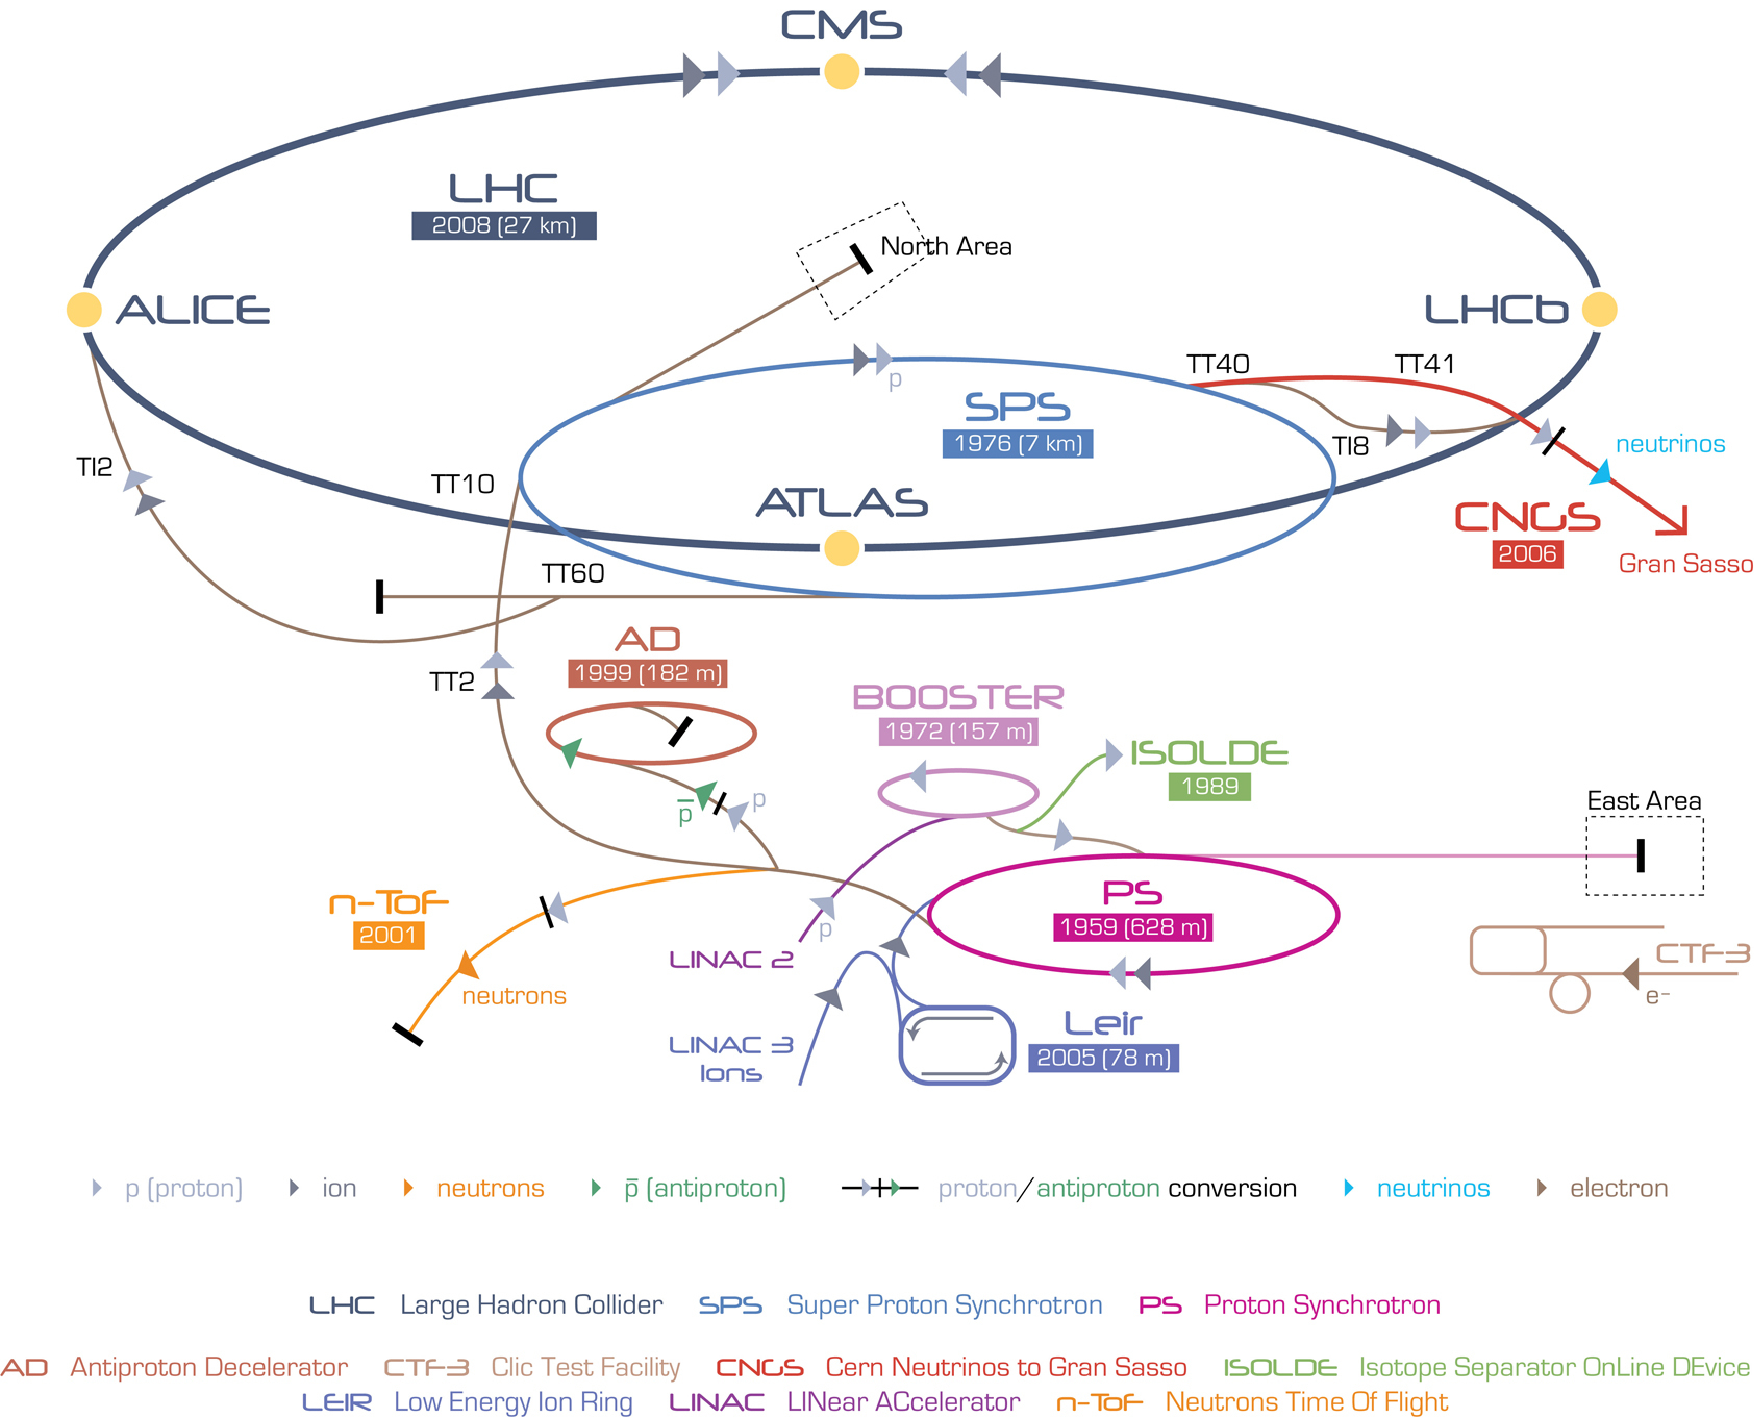
\includegraphics[width=\hugefigwidth]{chap_CMSDetector_figures/Cern-Accelerator-Complex}
  \caption[CERN accelerator complex]%
  {LHC  accelerator complex}
  \label{fig:CERNAccComplex}
\end{figure}




\begin{figure}
  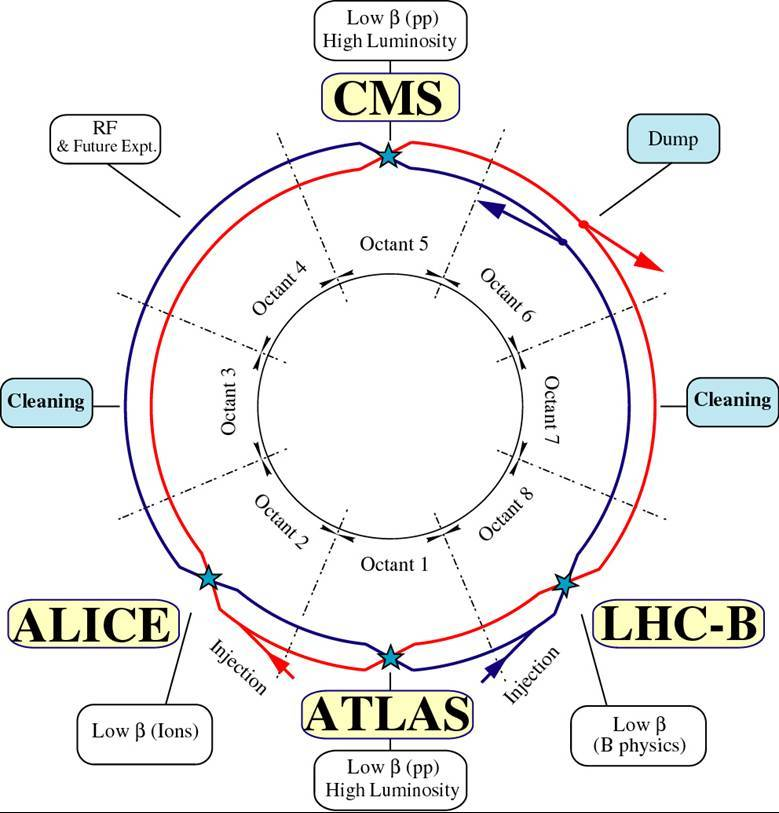
\includegraphics[width=\mediumfigwidth]{chap_CMSDetector_figures/lhc-schematic}
  \caption[LHC ring]%
  {LHC ring}
  \label{fig:LHCRing}
\end{figure}

It has circumference of 27 kms and is placed in a tunnel, 175 meters under the ground near Geneva.
The tunnel was originally built for the Large Electron-Positron collider \cite{LEP}. 
For the LHC operation, they have been upgraded to provide beams of protons for 
collisions at unprecedented energies. 
Technical limitations in the production and storage of antiprotons led to the de- 
cision to build a proton-proton collider. Accelerated electrons and positrons suffer 
large energy loss due to the synchrotron radiation, which is proportional to 
$\frac{E^4}{(Rm^4)}$, 
where E is the electron energy, m is the particle's mass and R the accelerator radius. 
Therefore, only massive charged particles could have been used, e.g. protons and 
heavy nuclei, in order to obtain energies of the order of TeV at the fixed accelerator 
radius. 

\subsection{The Accelerator Chain}

The LHC is constituted by 1232 super-conducting dipole magnets each 15 m long, 
delivering a 8.3 T magnetic field to let the beams circulate inside their trajectories 
along the 27 km circumference. Two vacuum pipes are utilized to let beams circulate 
in opposite directions. 
More than 8000 other magnets are utilized for the beam 
injection, their collimation, trajectory correction, crossing. All the magnets are kept 
cool by superfluid helium at 1.9 K temperature. The beams are accelerated from 
450 GeV (the injection energy from the SPS) to 7 TeV with 16 Radio Frequency 
cavities (8 per beam) which raise the beam energy by 16 MeV each round with an 
electric field of 5 MV/m oscillating at 400 MHz frequency. Before the injection into 
the LHC, the beams are produced and accelerated by different 26 components of the 
CERN accelerator complex. Being produced from ionized hydrogen atoms, protons 
are accelerated by the linear accelerator LINAC, Booster and the Proton Synchrotron 
(PS) up to 26 GeV energy, the bunches being separated by 25 ns each. The beams are 
then injected into the Super Proton Synchrotron (SPS) where they are accelerated 
up to 450 GeV. They are then finally transferred to the LHC and accelerated up to 
7 TeV energy per beam.


Figure \ref{fig:CERNAccComplex} shows the full CERN accelerator complex.


In addition to $p + p$ operation, the LHC had 
heavy nuclei $(Pb + Pb)$ collisions in 2009 and 2011 
 with an energy of 2.76 TeV per nucleon. The availability of high energy heavy-ion beams at energies
over 30 times higher than at the present other accelerators will allow us to
further extend the range of the heavy-ion physics program to include studies
of hot nuclear matter.


%\section{Lattice layout}
The two LHC symmetrical rings are divided into eight octants and arcs and
eight straight sections approximately 528 $m$ \ref{fig:LHCRing}. The two high luminosity
experimental insertions are located at diametrically opposite straight
sections: the A Toroidal LHC ApparatuS (ATLAS) experiment is located
at Point 1 and the Compact Muon Solenoid (CMS) experiment
at Point 5. The other two large experiments, A Large Ion Collider Experiment
(ALICE) and Large Hadron Collider beauty (LHCb), are located
at Point 2 and at Point 8, respectively, where the machine reaches a lower
luminosity of $L = 5 \, \times \,10^{32} cm^{-2}s^{-1}$. The remaining four straight sections do
not have beam crossings. The two beams are injected into the LHC in two
different octants, octant 2 and octant 8 respectively for clockwise and anticlockwise
beam. The octants 3 and 7, instead, contain two collimation systems
for the beam cleaning. 



\section{Luminosity}
The number of events per second generated in the LHC collisions is given by :
N = $L.\sigma$
where $\sigma$ is the cross section for the collisions process under study and $L$ the
machine luminosity. The machine luminosity depends only on the beam parameters and can be written, 
for a Gaussian beam distribution, as:

% thesisDongho ends

% PromptChic_CMS_2012.pdf 

\begin{equation}
\label{eq:Lumi}
L = \frac{n \cdot \,f_{rev}\cdot \,N_{1} \cdot \, N_{2}}{A^{eff}_T}
\end{equation}

where $A^{eff}_T$ is the effective transverse area of the proton beam, $n$ is the number of packets
the beam is splitted to and $f_{rev}$ is the frequency of revolution around the ring. $N_{1}$ and $N_{2}$ are
the number of protons in each packet. With respect to other high energy colliders, the design
luminosity of LHC is several magnitudes larger. This is needed because LHC is designed
to discover new particles at TeV scale. At these scales the interaction rates with momentum
transfers more than 1 TeV are very low. Therefore more data needs to be collected which can
only be achieved by having large luminosity.

% PromptChic_CMS_2012.pdf ends

% thesisDongho 
The LHC luminosity is not constant over physics a run, but decays due to the
degradation of intensities and emittance of circulating beams. The main cause
of the luminosity decay during normal LHC operation is the beam loss from
collisions.

\section{Compact Muon Solenoid}

The CMS experiment is a general purpose proton-proton detector designed to run 
at the highest luminosity of LHC. Figure \ref{fig:CMSFigure} gives a 3D structure view of the 
CMS detector.
The design of the CMS detector is based on a compact superconducting 
solenoid coupled with a muon detector system for optimized muon detection.
Superconducting solenoid provides a strong magnetic field of 3.8 $T$. 
Inside it, the inner tracking comprises a Pixel detector
surrounded by the Silicon Strip detector. Its high granularity (70
millions pixels, 10 millions strip) and precision ensures good track reconstruction
efficiency. It is surrounded by Electromagnetic calorimeter (ECAL) made
of 76000 lead tungstate crystals grouped in 36 barrel and 4 endcap supermodules.
The brass-scintillator sampling hadron calorimeter (HCAL) completes
the in-coil detectors. To ensure hermeticity the in-coil calorimetric system is
extended, away from the central dector, by the hadron outer detector (HO)
and a quartz fiber very forward calorimeter (HF) to cover $\eta le $< 5. Outside the
solenoid a muon system is built in the magnet steel return yoke. It's formed by
4 stations of muon chambers: Drift Tube (DT) in the barrel region, Cathode
Strip Chambers (CSC) in the endcap, Resistive Plate Chamber (RPC) in both
parts, providing muon detection redundancy. 







Two trigger levels are employed in CMS. The Level-1 Trigger (L1) is implemented using 
custom hardware processors and is designed to reduce the event rate to 100 kHz during LHC operation
using information from the calorimeters and the muon detectors. It operates nearly 
dead time-free and synchronously with the LHC bunch crossing
frequency of 40 MHz. The High Level Trigger (HLT) is implemented across a
large cluster of commodity computers referred to as the event filter farm, and
provides further rate reduction to $\mathcal{O}$(100) Hz using filtering software applied
to data from all detectors at full granularity. The overall dimension of CMS
are a length of 21.6 $m$, a diameter of 14.6 $m$ and a total weight of 12500 tons.


A slice of the transverse view of the CMS detector
is shown in Figure \ref{fig:CMSFigureSlice}. The principle of detection of charged and neutral particles in
the various sub-detectors is shown. All charged particles leave signals in the inner
tracking system. Electrons and photons deposit their energy in the electromagnetic
calorimeter. Charged Hadrons (K$^{\pm}$, $\pi^{\pm}$ ...) and neutrons deposit their energy in the
hadronic calorimeter. Muon is a particle which passes through calorimeters without
interacting much, but which leaves a track of its passage in the muon chambers.
Neutrinos, barely interacting, will escape from all direct detections. While adding
the transverse momenta of all the particles detected by the detector, one can determine
the imbalance of energy in the transverse plane, so called the missing transverse
energy.

\begin{figure}
  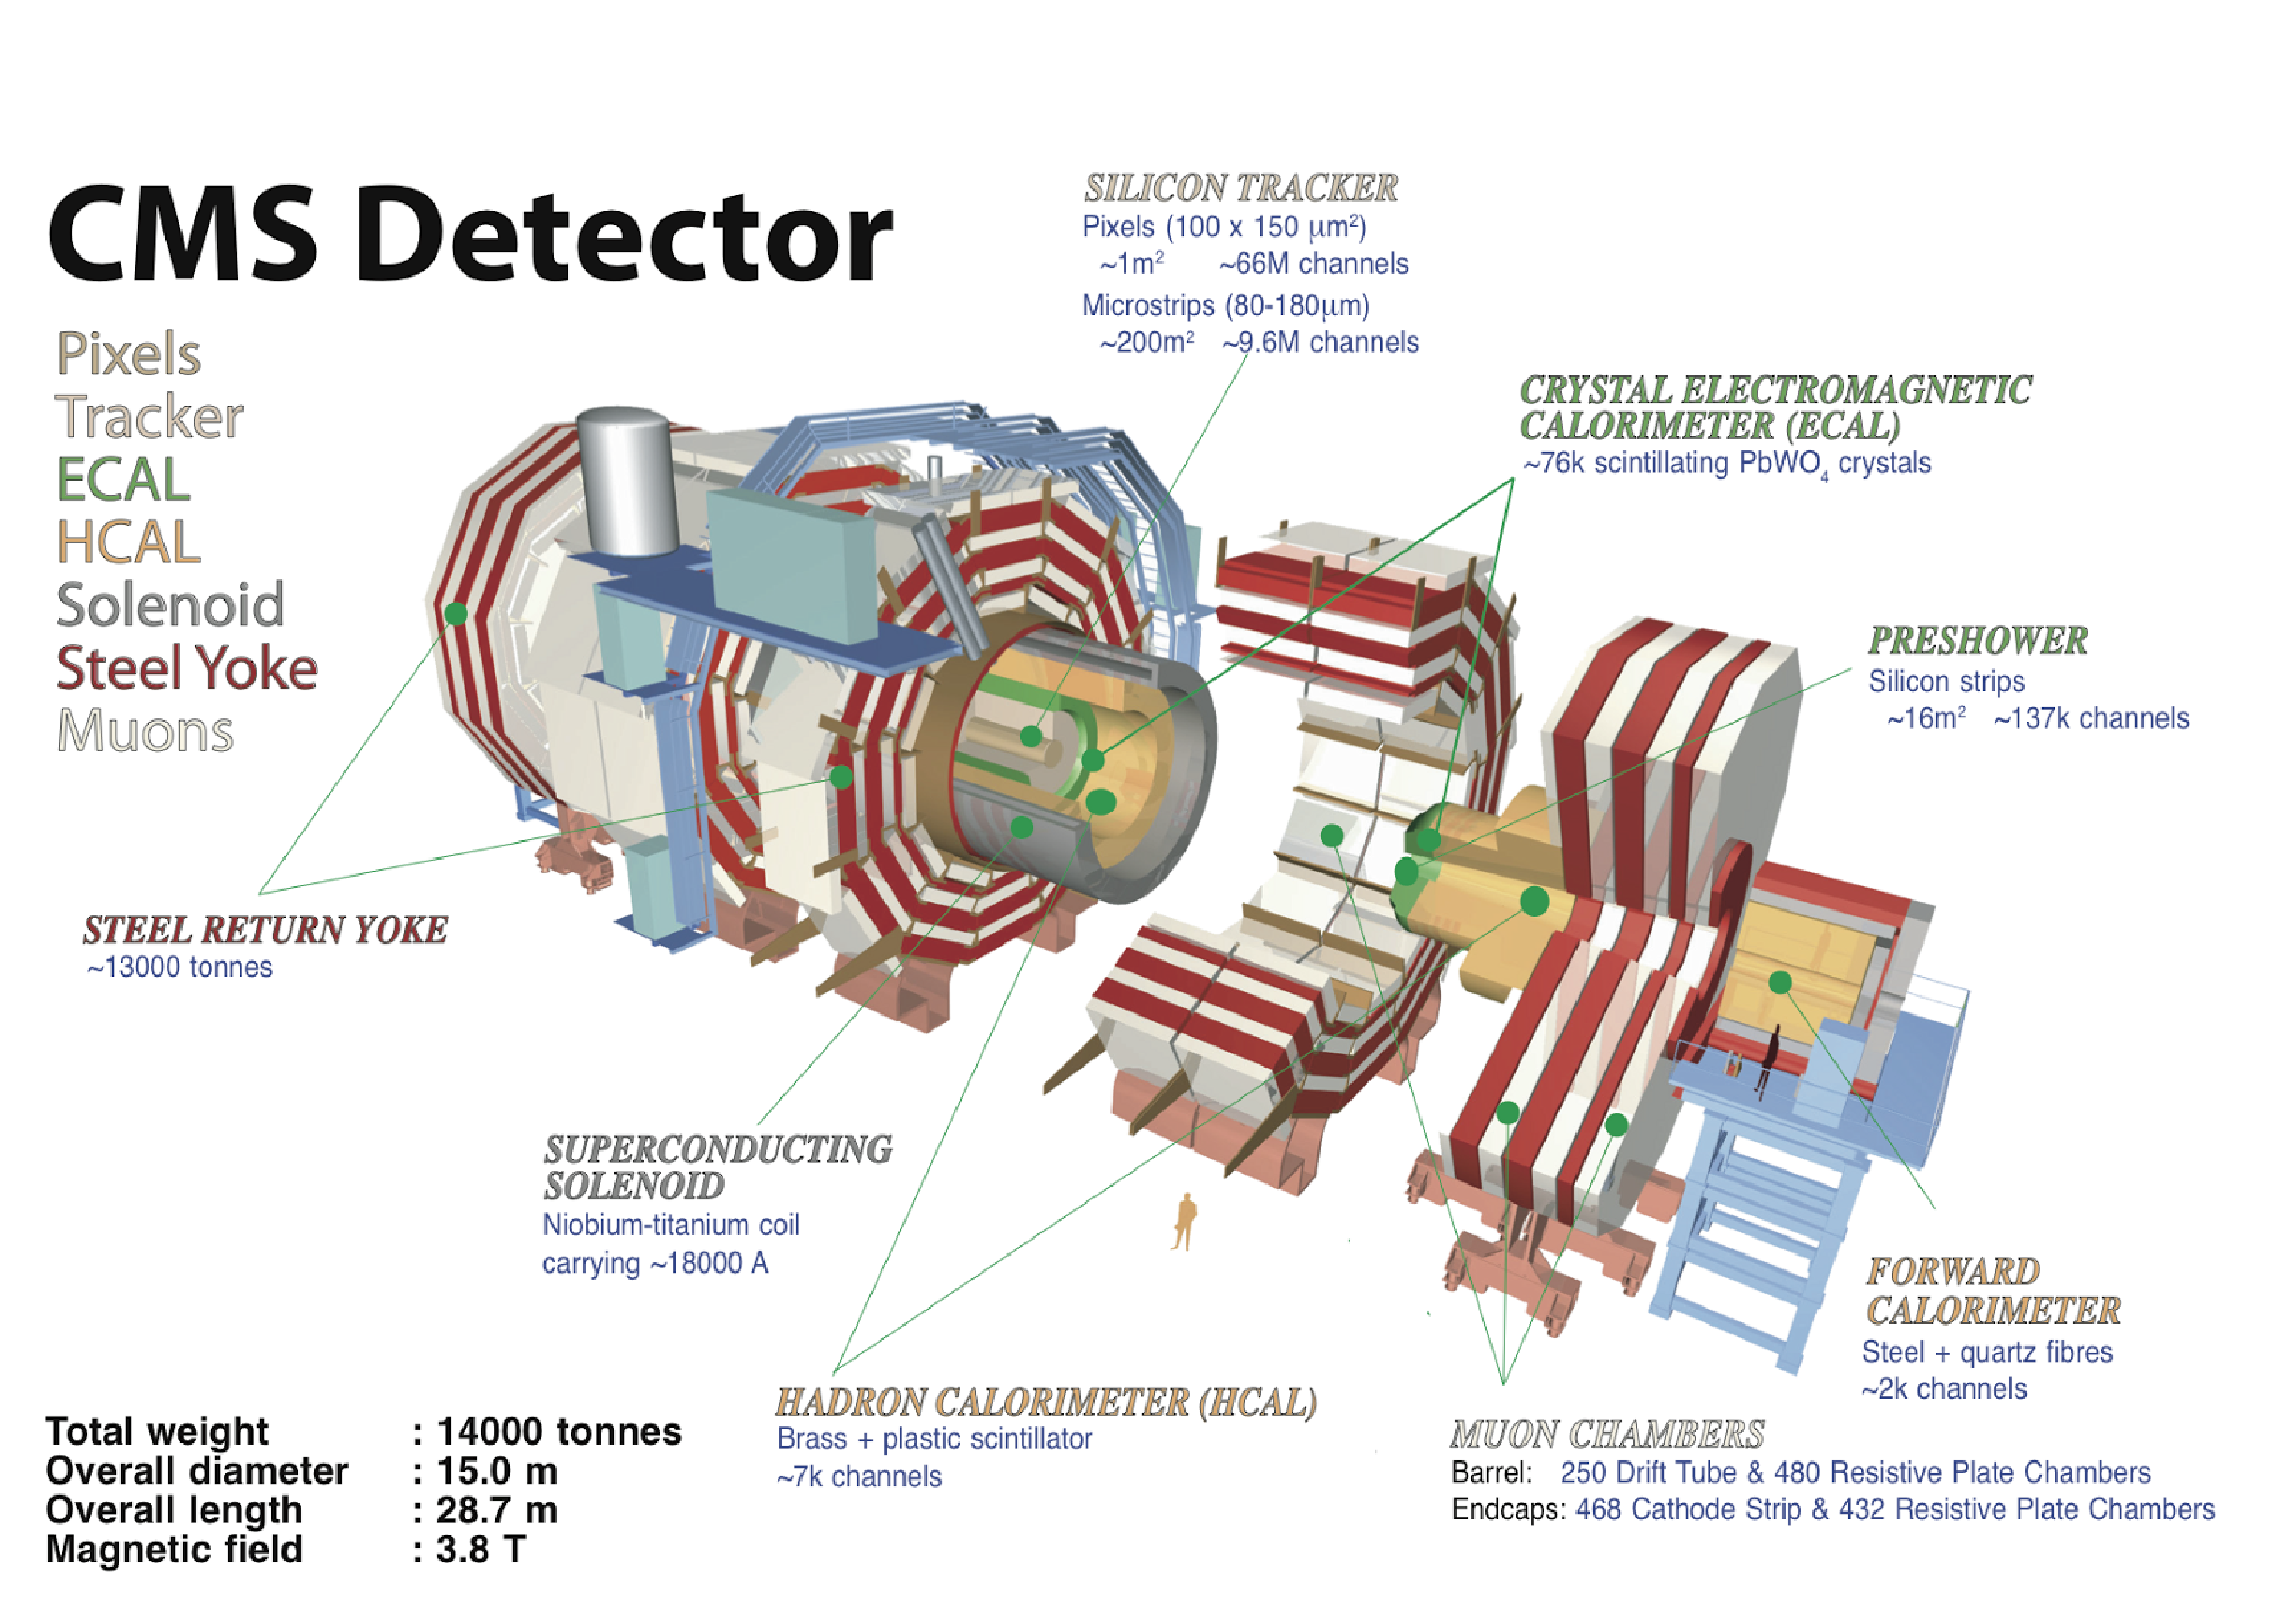
\includegraphics[width=\hugefigwidth]{chap_CMSDetector_figures/CMS}
  \caption[CMS Detector figure]%
  {CMS detector figure}
  \label{fig:CMSFigure}
\end{figure}



\begin{figure}
  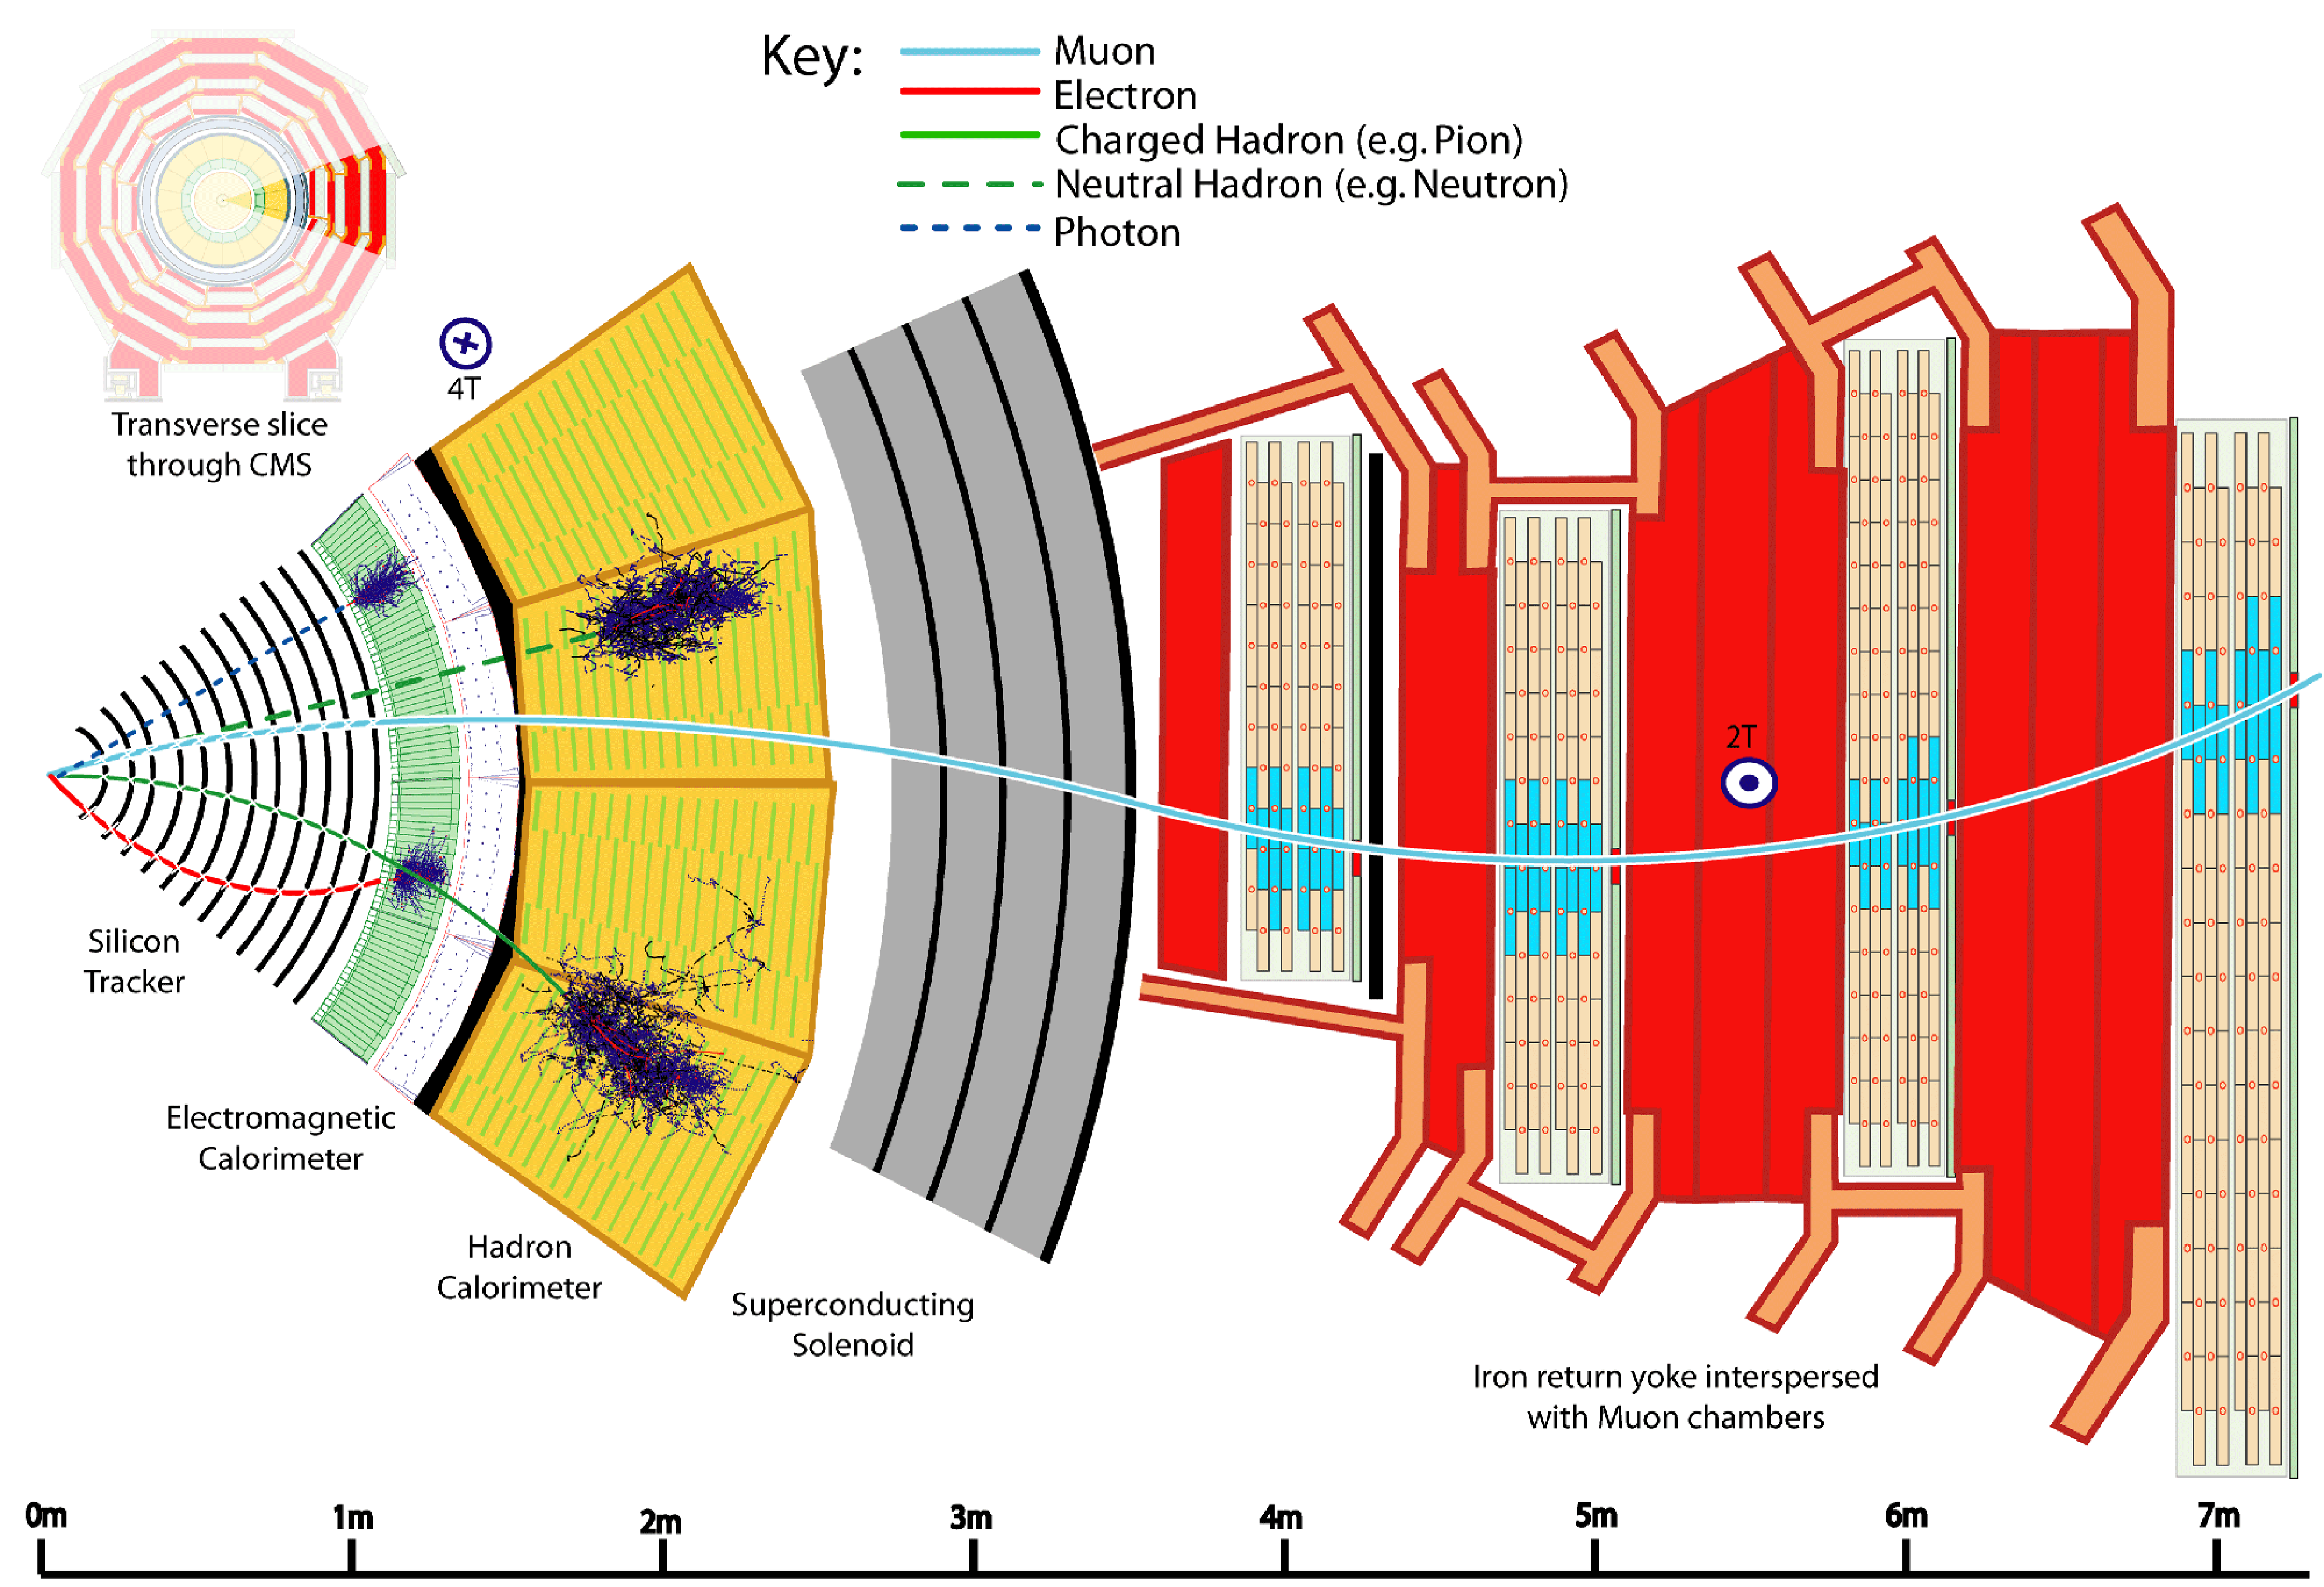
\includegraphics[width=\hugefigwidth]{chap_CMSDetector_figures/cms_slice}
  \caption[CMS Detector Slice figure]%
  {CMS detector figure slice}
  \label{fig:CMSFigureSlice}
\end{figure}

The coordinate system of CMS has its origin inside the detector at the primary
interaction point. The x-axis points radially towards the center of the
LHC, whereas the y-axis points vertically upward. Thus, the z-axis shares the
same direction with the beam line. The azimuthal angle $\phi$ is measured from
the x-axis in the x-y plane whereas the polar angle $\theta$ is measured from the z-axis.

Particle physicists often use a quantity called rapidity
$y$ instead of $\theta$. It is defined as:

\begin{equation}
\label{eq:CMSqd1}
 y = \frac{1}{2} \,\ln \frac{E + p_z}{E - p_z} \, = tanh^{-1} \,\frac{p_z}{E}
\end{equation}

and equals, in case of massless particles, the pseudorapidity $\eta $ given by

\begin{equation}
\label{eq:CMSqd2}
 \eta = -\ln[\tan(\theta/2)]
\end{equation}

The use of rapidity instead of the polar angle is motivated by the fact that the difference 
in rapidity between two particles is invariant under Lorentz boosts along the beam axis

The angular distance between two particles observed from the origin of the
coordinate system is

\begin{equation}
\label{eq:CMSqd3}
\Delta R = \sqrt{\Delta \phi^2 + \Delta \eta^2} 
\end{equation}

Measurable quantities like momentum and energy transverse to the beam line
are denoted by $p_T$ and $E_T$ , respectively, and can be derived from its x and
y components. The CMS detector is located north of the LHC center. The
origin of the CMS coordinate system is the CMS collision point. Neglecting
the small tilt of the LEP/LHC plane.

\subsection{Magnet}

The superconducting solenoid magnet reaches a maximum magnetic field of 3.8 
T in the positive z direction in the inner detectors. A high magnetic field provides 
a large bending power in the transverse plane for charged particles, which makes 
possible to reach precise measurement of muon momenta. The magnet is 12.5 m long 
and with an inner radius of 6 m and is made of four-layers of NbTi. It is the largest 
superconducting magnet ever built, with the capacity to store an energy of 2.6 GJ at 
full current. The magnetic flux is returned via a 1.5 m thick iron yoke instrumented 
with four stations of muon chambers. In this part of the detector the magnetic field 
is saturated at 2 T. More detailed information can be found in reference \cite{CMSMagnet} 
Figure \ref{fig:CMSMagnet} shows artistic view of CMS magnet, a huminoid is also persent
on figure to highlight the huge size of magnet.
\begin{figure}
  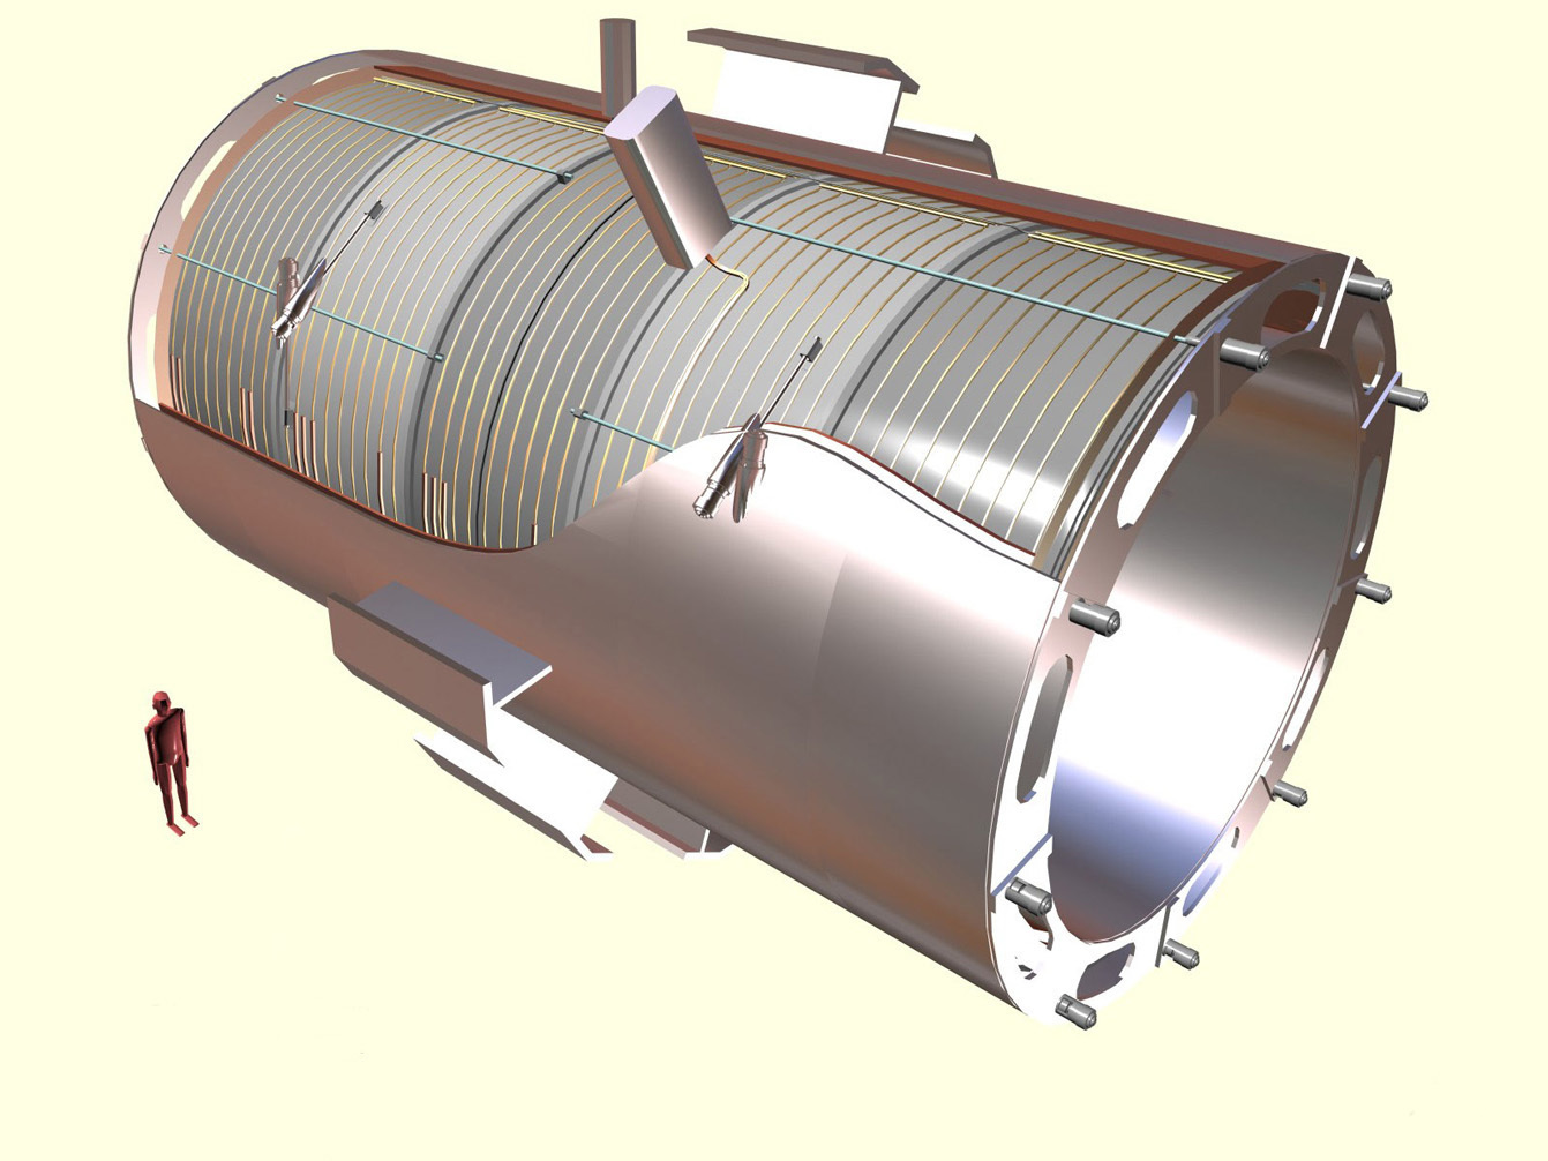
\includegraphics[width=\largefigwidth]{chap_CMSDetector_figures/cms_magnet}
  \caption[CMS Magnet artistic view]%
  {CMS Magnet }
  \label{fig:CMSMagnet}
\end{figure}



\subsection{Tracker}

The Tracker is the subdetector system which is closest to the interaction point, 
a general layout is presented in Figure \ref{fig:CMSTracker} It is designed to provide an efficient mea- 
surement of the trajectories of charged particles emerging from the LHC collisions, as 
well as a precise reconstruction of secondary vertices. The CMS Tracking System is 
composed of q silicon pixel detector close to the interaction region and a strip detector 
covering radii from 0.2 m to 1.1 m. The Pixel Detector consists of 1440 pixel modules 
arranged in three barrel layers and two disks in each end-cap. The barrel layers are 
located at radii of 4.4, 7.3 and 10.2 cm around the interaction point with a length of 
53 cm. On each side of the barrel, two discs are placed at $|z|$ = 32.5 cm and 46.5 cm.

\begin{figure}
  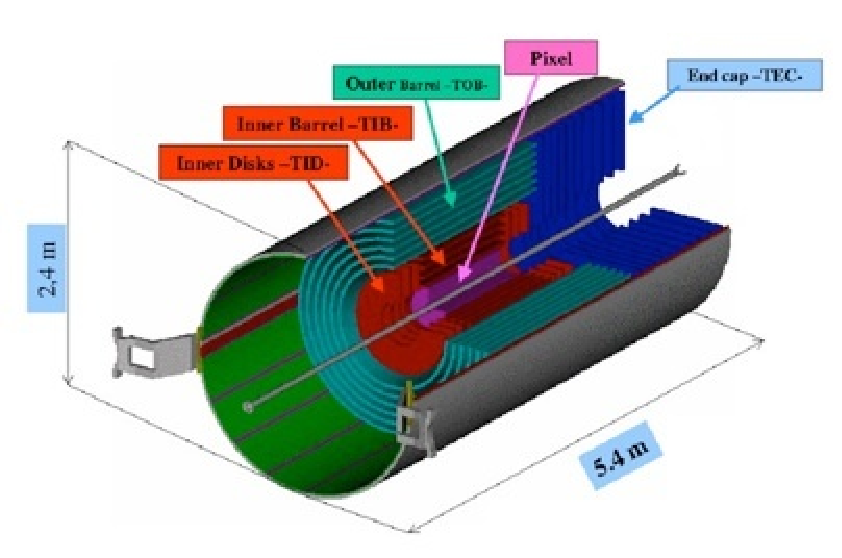
\includegraphics[width=\largefigwidth]{chap_CMSDetector_figures/cms_tracker_3d_drawing}
  \caption[CMS Tracker 3D drawing]%
  {CMS Tracker drawing}
  \label{fig:CMSTracker}
\end{figure}


\subsection{Calorimetry}

{\bf ECAL} \\


The electromagnetic calorimeter (ECAL) is used to measure the energy of photons 
and electrons. The ECAL is a high precision scintillating crystal calorimeter. The 
structure of the ECAL can be seen in Figure \ref{fig:CMSECAL}. It is composed of 61,200 lead tungstate 
(PbWO$_4$) crystals in the barrel region and 7,324 crystals in the endcaps. The choice 
of that material is motivated by its fast response and high radiation resistance and 
its very good resolution. In front of each ECAL Endcap is a preshower detector (ES),
from 1.65 $ \leq |\eta| \leq$ 2.6 made from silicon strip detectors in order to identify neutral 
pions ($\pi^0$). The nominal energy resolution, measured with electron beams having 
momenta between 20 and 250 GeV, is:
 
\begin{equation}
\label{eq:eqnECAL}
%\Delta R = \sqrt{\Delta \phi^2 + \Delta \eta^2} 
\frac{\sigma_E}{E}=(\frac{S}{\sqrt{E}})^2 + (\frac{N}{E})^2 + C^2.
\end{equation}


where S is the stochastic term, which includes fluctuations in the shower containment 
as well as a contribution from photostatistics, N is the noise term, which accounts 
for the electronic, digitization, and pileup noise, and C is the constant term, which 
comes from the light collection non-uniformity, errors on the inter-calibration among 
the modules, and the energy leakage from the back of the crystal.\\

\begin{figure}
  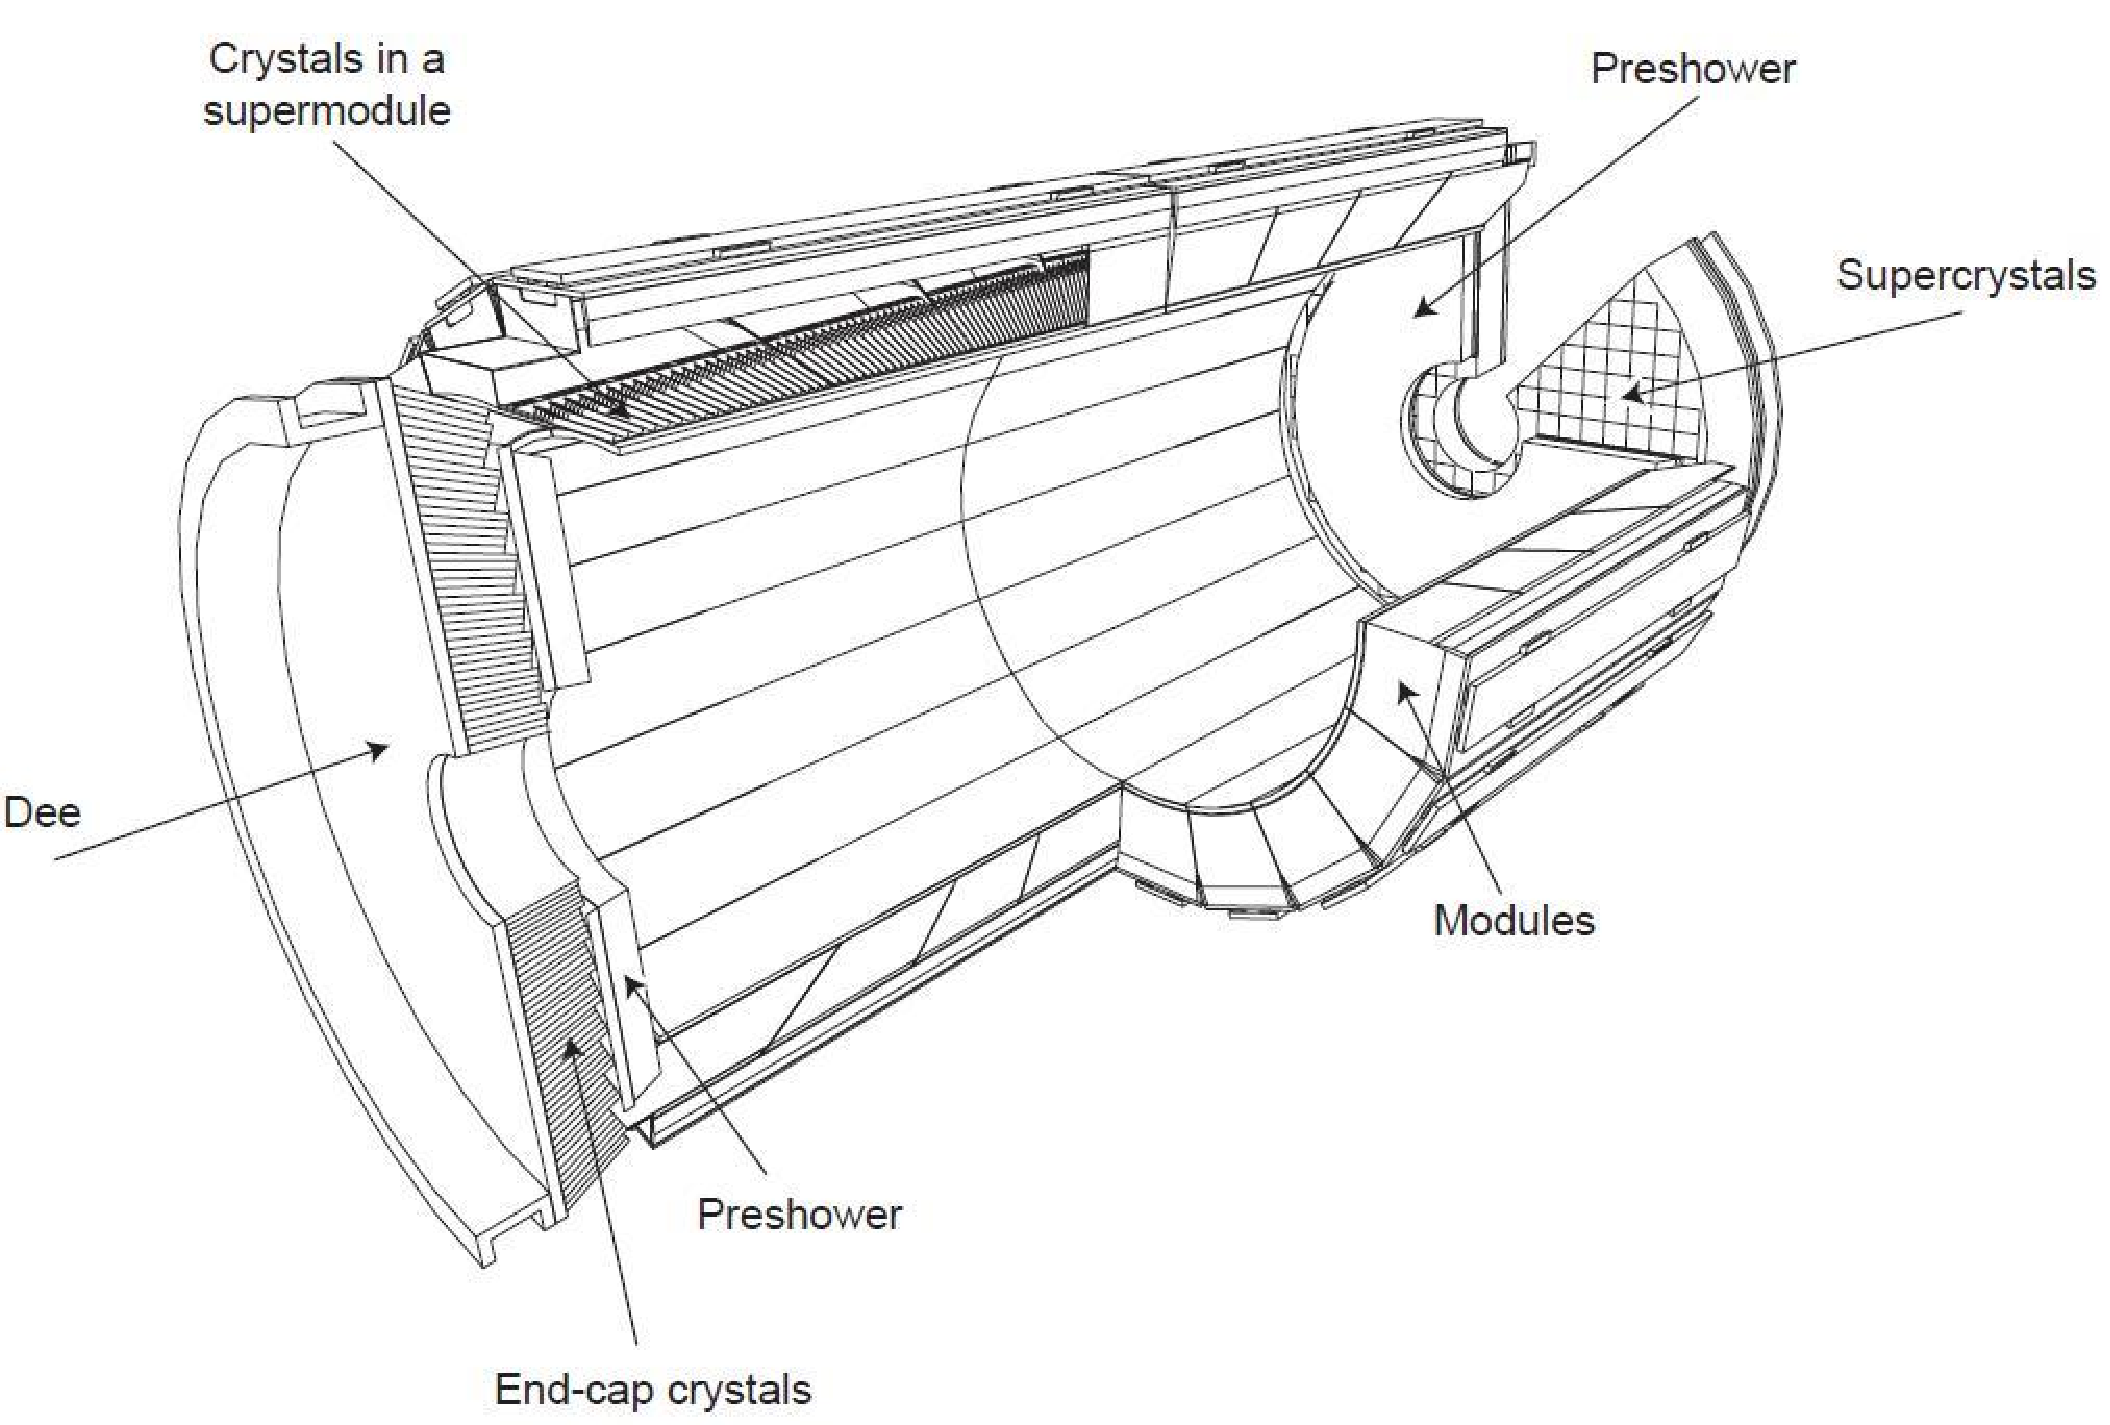
\includegraphics[width=\largefigwidth]{chap_CMSDetector_figures/cms_ECAL}
  \caption[CMS ECAL]%
  {CMS ECAL detector}
  \label{fig:CMSECAL}
\end{figure}


{\bf HCAL}  \\

The hadronic calorimeter (HCAL) is designed to measure the energy of hadrons. 
The HCAL is comprised of four subsystems: the HCAL Barrel (HB), the outer 
calorimeter (HO), the HCAL Endcap (HE), and the forward calorimeter (HF). 
Figure \ref{fig:CMSHCAL} gives a schematic overview on the HCAL sub-detector. 
The HB is a sampling calorimeter that covers the range $|\eta| < $ 1.3. 
It consists of 36 identical azimuthal wedges aligned parallel to the beamline. 
It is located between the ECAL and the 
solenoid coil and is supplemented by the HO located between the solenoid and the 
muon chambers. The HO is designed to absorb the remnant of the hadronic shower 
which has not been fully absorbed in the HB. The HE covers a large portion of the 
solid angle, 1.3 $< |\eta| < 3$. Beyond that region, the HF placed at 11.2 m from the 
interaction point extends the pseudorapidity coverage up to $|\eta|$ < 5.2. The HE must 
have high radiation tolerance, with 10 Mrad expected after 10 years of operation. 
The reason for the absorber material to be non-magnetic is that it must not affect 
the magnetic field. The HF experiences the harshest radiation environment and therefore 
requires an extremely radiation tolerant material. The active material chosen is 
quartz fibers.
The fibers are mounted in grooves in the steel absorber plates. The inner part of the HF will be 
exposed to close to 100 Mrad/year. As the absorber will become radioactive the entire HF can be moved into
a garage to limit exposure of personnel during maintenance periods.


\begin{figure}
  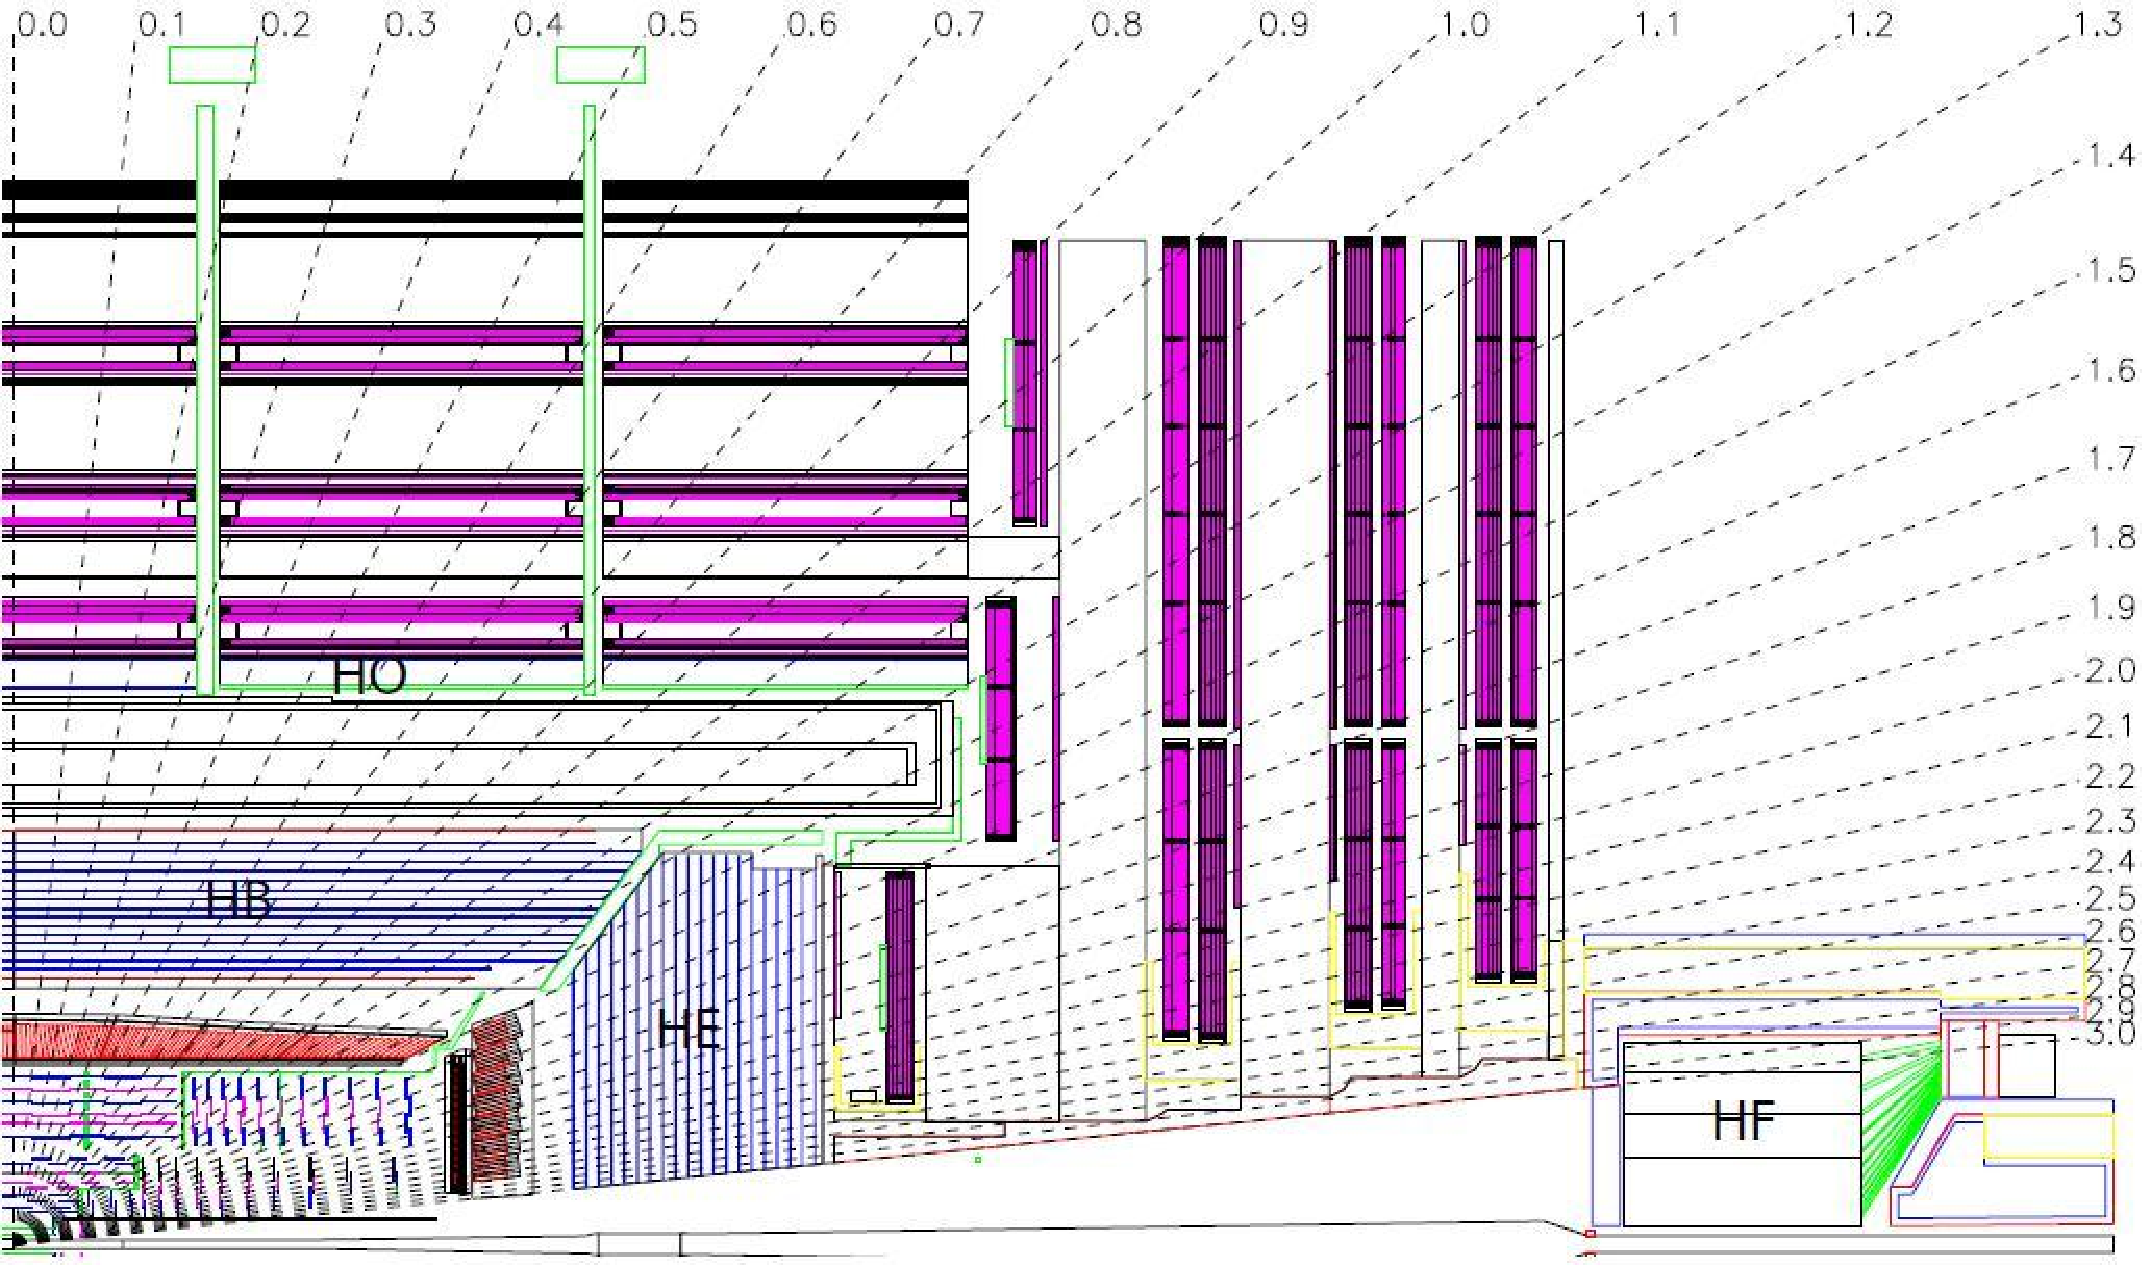
\includegraphics[width=\largefigwidth]{chap_CMSDetector_figures/cms_HCAL}
  \caption[CMS HCAL]%
  {CMS HCAL detector}
  \label{fig:CMSHCAL}
\end{figure}


\subsection{CMS Muon System}

One of the main design objectives of the CMS detector was to obtain a high precision
muon momentum measurement, for its key role both in new physics searches and
in Standard Model measurements. The CMS muon system \cite{CMSExp} uses three diffrent
types of gaseous detectors to detect muons. In the barrel region, Drift Tubes (DTs)
and Resistive Plate Chambers (RPCs) are used, while in the endcap there are Cathode
Strip Chambers (CSCs) and also RPCs. The layout of the CMS muon system is shown in 
Figure \ref{fig:CMSMuonSystem}. \\



\begin{figure}
  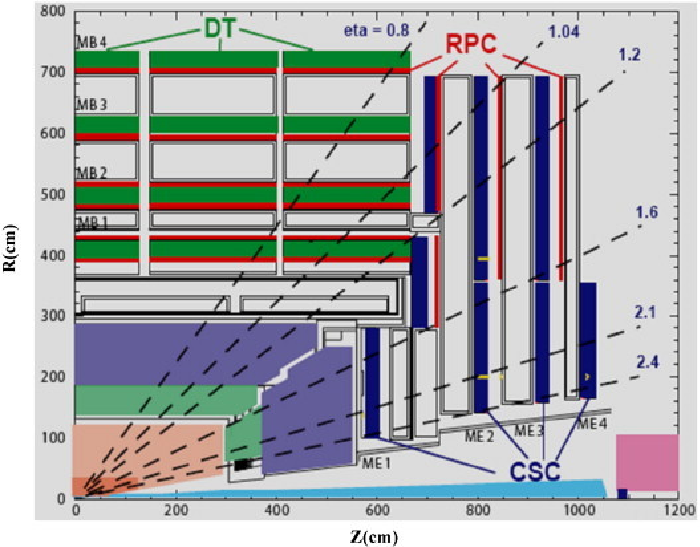
\includegraphics[width=\largefigwidth]{chap_CMSDetector_figures/CMSMuonSystem}
  \caption[CMS Muon system]%
  {CMS Muon system}
  \label{fig:CMSMuonSystem}
\end{figure}


{\bf Drift Tubes} \\

In the central region of CMS, $|\eta| <$ 1.2, the muon system consists of four concentric
cylinders containing 250 gas drift chambers. Each Drift Tube is filled will a mix of
85$\%$ Argon and 15$\%$ CO$_2$ with active wires for charge collection. As muons pass
through the gas they leave an ionization trail. The charge drifts to the wires, which
detect the charge. The size of the drift cell was chosen so the maximum drift time is
380 ns. There are $~$172000 active wires in the entire system. The use of DTs is only
possible in this region due its low magnetic field.\\


{\bf Cathode Strip Chambers} \\

In the endcap, the muon system is comprised of Cathode Strip Chambers (CSC).
The CSC's cover the 0.9$<|\eta|<$2.4 pseudorapidity range. Each CSC is trapezoidal
in shape and consists of 6 gas gaps, each gap having a plane of radial cathode strips
and a plane of anode wires running almost perpendicularly to the strips. The CSC is
a fast detector (response time of $~$4.5 ns), but with rather coarse position resolution;
a precise position measurement is made by determining the centre-of-gravity of the
charge distribution induced on the cathode strips (spatial resolution $~$200 $\mu$m, angular
resolution $~$10 mrad).\\


{\bf Resistive Plate Chambers} \\

In order to improve muon trigger system and for a good measurement of the bunch
crossing time, resistive plate chambers (RPC) are mounted in the barrel and endcap
region ($|\eta| < $1.6). The RPCs are able to provide independent and fast trigger with
high segmentation and sharp pT threshold over a large portion of the pseudorapidity
range. However, the RPCs have coarser position resolution making them more useful
for the trigger

\subsection{Trigger and Data Acquisition}

The CMS trigger system is designed to cope with an unprecedented high luminosity
and interactions rates. The LHC will collide proton bunches at a rate of 40
MHz which leads to $~$10$^9$ interactions per second at design luminosity. Since it is
not possible to record events at this rate, a two-part trigger system, consisting of a
hardware-based trigger (Level 1) and a software-based trigger (High Level Trigger) is
used \cite{CMSTrigger1,CMSTrigger2}. The rate is then reduced by a factor of 10$^6$.\\


{\bf Level 1 Trigger} \\
The Level 1 (L1) trigger is designed to achieve a maximum output rate of 100
kHz and consists of custom-designed, programmable electronics. The front-end (FE)
electronics can store information from up to 128 consecutive events, which equates
to $~$3 $\mu$s. To cope with the time limitation, the L1 trigger system uses only coarsely
segmented data from the muon system and the calorimeters while the full granularity
data are stored in the FE electronics waiting for the L1 decision. The L1 muon trigger
is organized into subsystems representing the three different muon detectors: the DT
trigger in the barrel, the CSC trigger in the endcap and the RPC trigger covering
both barrel and endcap. The Level-1 muon trigger also has the Global Muon Trigger
(GMT) that combines the trigger information from the DT, CSC, and RPC muon
subsystems, as well as from the calorimeter subsystem, and sends it to the Level-1
Global Trigger.\\


{\bf High Level Trigger }\\

The High Level Trigger (HLT) exploits the full amount of collected data for each
bunch crossing accepted by Level 1 Trigger and is capable of complex calculations
such as the offine ones. It is structured in two levels, Level 2 (L2) and Level 3
(L3) implemented in software. The L2 uses information from the muon spectrometer
(parameters from the L1 muon candidates converted into seeds) to perform a standalone
reconstruction, providing a muon pT measurement with a precision of about
15 $\%$. The L2 reconstruction follows closely the offine standalone reconstruction using
Kalman-filter techniques. The L3 takes L2 candidates as seeds and adds information
from the inner tracker by performing track reconstruction in the silicon tracker. This
reconstruction is regional, it performs pattern recognition and track fitting only in
a small $\eta - \phi $ slice of the tracker, to keep execution time low. Trajectories are then
reconstructed using Kalman-filter techniques. Level 3 provides a much more precise
p$_T$ measurement (1$\%$ - 2$\%$ in the barrel region) than Level 2, as well as the ability
to select on the basis of the track impact parameter with respect to the beam spot.
After the HLT decisions, the event rate decreases down to 100Hz for mass storage
which corresponds to a data rate of 150 Mbyte$/$s.


\subsection{CMS data flow}
Raw data that passed HLT and CMS Online Data Acquisition system (system which collects
data from different detectors and builds events) is stored at a storage facility at CERN, known
as Tier-0. The raw data contains information for every single proton-proton collision which
passed HLT and it is called an event. There are about 10$^9$ events per year stored at Tier-0.
Standard CMS algorithms perform calibration and alignment of the detector using raw data
and do prompt (first) reconstruction of physics objects like muons, electrons, jets etc. Later,
their momenta, energies and trajectories are measured and this is done by using all detectors
of CMS experiment.
The output data from prompt reconstruction is saved in different primary datasets based on
trigger information.
The data from Tier-0 is transferred to Tier-1 storage facilities worldwide where further calibration
and re-reconstruction is performed centrally to be used by all CMS analyzes. The
Tier-2 centers are more numerous and they are based at different universities in the world.
They have limited disk space and are used for running individual analysis and Monte Carlo
simulations.
Data is stored in three types of root files which contain information about raw, reconstructed
and analysis object data, respectively RAW, RECO and AOD root files. The RAW root files
contain information about the recorded event in raw format as hits, energy deposits in the detector
etc. The RECO root files contain detailed information of reconstructed physics objects
and the AOD root files are simplified version of the RECO files which are mostly used in the
analyses.
Tier-0, Tier-1 and Tier-2 centers form a GRID \cite{LHCGrid} based computer infrastructure in 35 countries.


  \chapter{$\Upsilon$ production in Pb+Pb collisions}
\label{chap:UpsilonProductionPbPb}

\section{$\Upsilon(nS)$ in Pb+Pb collisions}
At large energy densities and high temperatures, strongly interacting
matter consists of a deconfined and chirally-symmetric system of
quarks and gluons~\cite{Karsch:2003jg}. This state, often referred to
as ``quark-gluon plasma'' (QGP)~\cite{Shuryak:1977ut}, constitutes the
main object of the studies performed with relativistic heavy-ion
collisions~\cite{Arsene:2004fa,Back:2004je,Adcox:2004mh,Adams:2005dq}.

The formation of a QGP in high-energy nuclear collisions can be
evidenced in a variety of ways. One of its most striking expected
signatures is the suppression of quarkonium
states~\cite{SATZ}, both of the charmonium (\Jpsi, $\psi'$,
$\chi_c$, etc.) and the bottomonium ($\PgU\text{(1S,\,2S,\,3S)}$,
$\chi_b$, etc.) families.  This is thought to be a direct effect of
deconfinement, when the binding potential between the constituents of
a quarkonium state, a heavy quark and its antiquark, is screened by
the colour charges of the surrounding light quarks and gluons.  The
suppression is predicted to occur above the critical temperature of
the medium ($T_c$) and depends on the \QQbar binding energy. Since the
\PgUa\ is the most tightly bound state among all quarkonia, it is
expected to be the one with the highest dissociation
temperature. Examples of dissociation temperatures are given in
Ref.~\cite{Mocsy:2007jz}: $T_{\text{dissoc}}\sim\!1\,T_c$, $1.2\,T_c,$
and $2\,T_c$ for the \PgUc, \PgUb, and \PgUa, respectively. Similarly,
in the charmonium family the dissociation temperatures are
$\leq1\,T_c$ and $1.2\,T_c$ for the $\psi'$ and \Jpsi,
respectively. However, there are further possible changes to the
quarkonium production in heavy-ion collisions. On the one hand,
modifications to the parton distribution functions inside the nucleus
(shadowing) and other cold-nuclear-matter effects can reduce the
production of quarkonia without the presence of a
QGP~\cite{Vogt:2010aa,Zhao:2011cv}. On the other hand, the large
number of heavy quarks produced in heavy-ion collisions, in particular
at the energies accessible by the Large Hadron Collider (LHC), could
lead to an increased production of quarkonia via statistical
recombination~\cite{Zhao:2010nk,Andronic:2006ky,Capella:2007jv,Thews:2005vj,Yan:2006ve,Grandchamp:2005yw}.

Charmonium studies in heavy-ion collisions have been carried out for
25 years, first at the Super Proton Synchrotron (SPS) by the
NA38~\cite{Baglin:1994ui},
NA50~\cite{Alessandro:2004ap,Alessandro:2006ju}, and
NA60~\cite{Arnaldi:2007zz} fixed-target experiments at 17.3--19.3\GeV
centre-of-mass energy per nucleon pair (\sqrtsnn), and then at the
Relativistic Heavy Ion Collider (RHIC) by the PHENIX experiment at
\sqrtsnn = 200\GeV~\cite{Adare:2006ns}. In all cases, \Jpsi
suppression was observed in the most central collisions. At the SPS,
the suppression of the $\psi'$ meson was also
measured~\cite{Alessandro:2006ju}. Experimentally, the suppression is
quantified by the ratio of the yield measured in heavy-ion collisions
and a reference. At RHIC, the reference was provided by the properly
scaled yield measured in \pp collisions. Such a ratio is called the
nuclear modification factor, \raa. In the absence of modifications,
one would expect \raa = 1 for hard processes, which scale with the
number of inelastic nucleon-nucleon collisions. For bottomonia, the
production cross section is too small at RHIC to make definitive
statements~\cite{Abelev:2010am}. With the higher energy and luminosity
available at the LHC, new studies for charmonia and bottomonia have
become possible. 

\section{Data Selection}
\label{sec:data-selection}
\subsection{Event Selection}
\label{sec:event-sel}

Inelastic hadronic \PbPb collisions are selected using information
from the BSC and HF calorimeters, in coincidence with a bunch crossing
identified by the beam pick-up (one on each side of the interaction
point)~\cite{Adolphi:2008zzk}.  Events are further filtered offline by
requiring a reconstructed primary vertex based on at least two tracks,
and at least 3 towers on each HF with an energy deposit of more than
3\GeV per tower. These criteria reduce contributions from single-beam
interactions with the environment (e.g. beam-gas collisions and
collisions of the beam halo with the beam pipe), ultra-peripheral
electromagnetic interactions, and cosmic-ray muons. A small fraction
of the most peripheral PbPb collisions are not selected by these
\emph{minimum-bias} requirements, which accept $(97\pm3)$\% of the
inelastic hadronic cross section~\cite{Chatrchyan:2011sx}. A sample
corresponding to 55.7 M minimum-bias events passes all these
filters. Assuming an inelastic \PbPb cross section of $\sigma_{\PbPb}
= 7.65$~b~\cite{Chatrchyan:2011sx}, this sample corresponds to an
integrated luminosity of $\int L = 7.28\mubinv$. This
value is only mentioned for illustration purposes; the final results
are normalized to the number of minimum-bias events.

The measurements reported here are based on dimuon events triggered by
the L1 trigger, a hardware-based trigger that uses information
from the muon detectors. The CMS detector is also equipped with a
software-based high-level trigger (HLT). However, no further
requirements at the HLT level have been applied to the L1 muon objects
used for this analysis.

The event centrality distribution of minimum-bias events is compared
to events selected by the double-muon trigger in
\fig{fig:centrality}. The centrality variable is defined as the
fraction of the total cross section, starting at 0\% for the most
central collisions. This fraction is determined from the distribution
of total energy measured in both HF
calorimeters~\cite{Chatrchyan:2011pb}. Using a Glauber-model
calculation as described in Ref.~\cite{Chatrchyan:2011sx}, one can
estimate variables related to the centrality, such as the number of
nucleons participating in the collisions (\npart) and the nuclear
overlap function (\taa), which is equal to the number of elementary
nucleon-nucleon (NN) binary collisions divided by the elementary NN
cross section and can be interpreted as the NN equivalent integrated
luminosity per heavy ion collision, at a given
centrality~\cite{Miller:2007ri}. The values of these variables are
presented in \tab{tab:glauber} for the centrality bins used in this
analysis. The double-muon-triggered events are more frequent in
central collisions since the main physics processes that generate
high-p$_T$ muon pairs scale with the number of inelastic nucleon-nucleon
collisions. In the following, \npart will be the variable used to show
the centrality dependence of the measurements.

\begin{figure}[hbtp]
  \begin{center}
   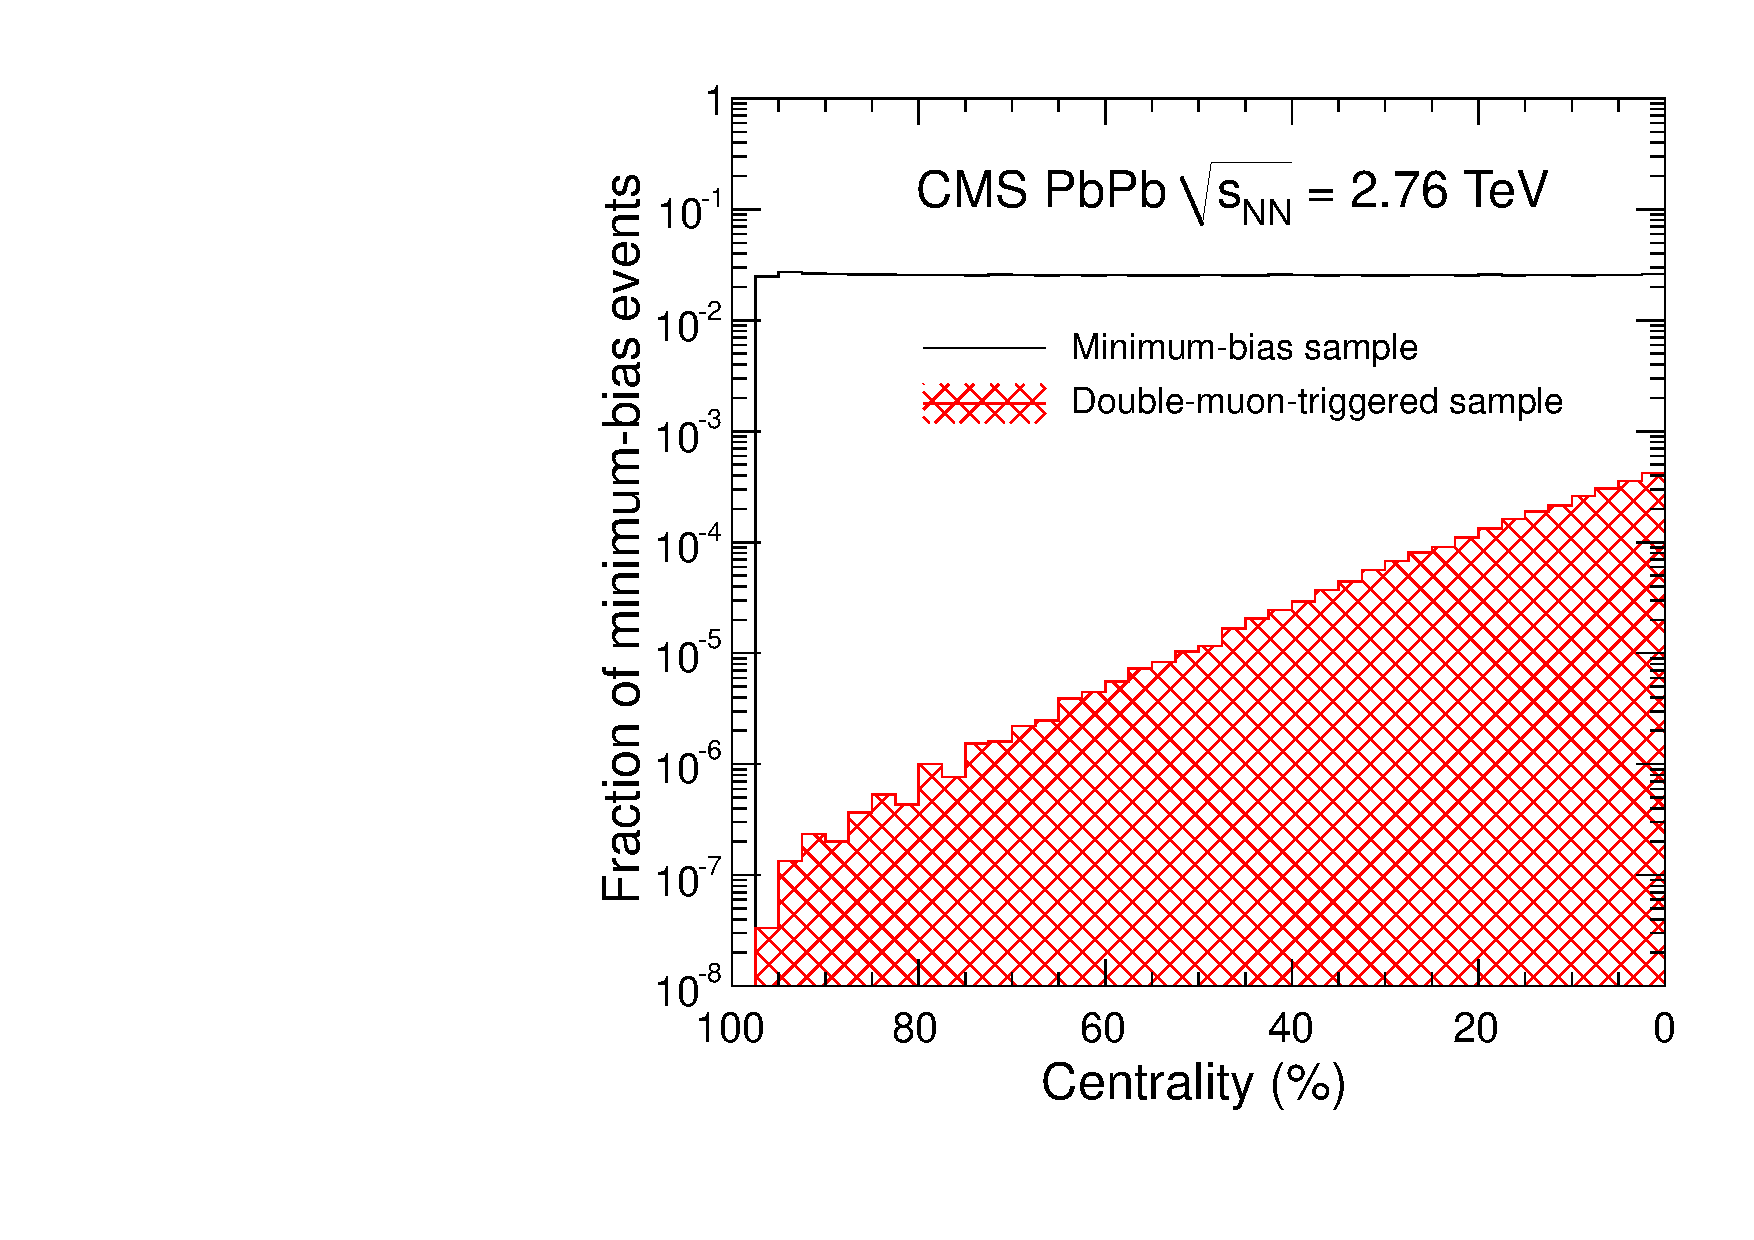
\includegraphics[width=0.5\linewidth]{chap_YInPbPbColl2010_figures/centralityDoubleMuOpen}
   \caption{Centrality distribution of the minimum-bias sample (solid
     black line) overlaid with the double-muon triggered sample
     (hashed red) in bins of 2.5\%.}
   \label{fig:centrality}
  \end{center}
\end{figure}




\begin{table}[htbp]
  \begin{center}
    \caption{Average and root-mean-square (RMS) values of the number of
      participating nucleons (\npart) and of the nuclear overlap function
      (\taa) for the centrality bins used in this
      analysis~\cite{Chatrchyan:2011sx}.}
    \label{tab:glauber}
    \begin{tabular}{rr@{.}lr@{.}lr@{.}lr@{.}lr@{.}lr@{.}lr@{.}lr@{.}l}
      \hline\vspace{0.1em}
      ~ & \multicolumn{4}{c}{$\npart$} &
      \multicolumn{4}{c}{$\taa$ (mb$^{-1}$)}\\
      Centrality (\%) & \multicolumn{2}{c}{Mean} & \multicolumn{2}{c}{RMS} & \multicolumn{2}{c}{Mean} & \multicolumn{2}{c}{RMS} \\\hline
      0--10	& 355&4 & 33&3 & 23&19 & 3&77 \\
      10--20	& 261&4 & 30&4 & 14&48 & 2&86 \\
      20--30	& 187&2 & 23&4 & 8&78  & 1&94 \\
      30--40	& 130&0 & 17&9 & 5&09  & 1&27 \\
      40--50	& 86&3  & 13&6 & 2&75  & 0&80 \\
      50--100	& 22&1  & 19&3 & 0&47  & 0&54 \\\hline
      0--20	& 308&4 & 56&8 & 18&83 & 5&49 \\
      20--100	& 64&2  & 63&0 & 2&37  & 3&05 \\\hline
      0--100	& 113&1 &115&6 & 5&66  & 7&54 \\\hline
    \end{tabular}
  \end{center}
\end{table}

\PgUa
Simulated MC events are used to tune the muon selection criteria, to
compute the acceptance and efficiency corrections, and to obtain
templates of the decay length distribution of \Jpsi from b-hadron
decays.  For the acceptance corrections described in
Section~\ref{sec:acc}, three separate MC samples, generated over full
phase space, are used: prompt J/$\psi$, J/$\psi$ from b-hadron decays,
and \PgUa. Prompt \Jpsi and \PgUa  are produced using PYTHIA
6.424~\cite{Sjostrand:2006za} at \sqrts = 2.76\TeV, which generates
events based on the leading-order colour-singlet and colour-octet
mechanisms, with non-relativistic quantum chromodynamics (QCD) matrix
elements tuned~\cite{Bargiotti:2007zz} by comparison with CDF data
~\cite{Acosta:2004yw}. The colour-octet states undergo a shower
evolution. For the non-prompt \Jpsi studies, the b-hadron events
are produced with PYTHIA in generic QCD 2$\rightarrow$2 processes. In
all three samples, the \Jpsi or \PgUa\ decay is simulated using the
EVTGEN~\cite{Lange:2001uf} package. Prompt \Jpsi and \PgUa\ are
simulated assuming unpolarized production, while the non-prompt \Jpsi
polarization is determined by the sum of the exclusive states
generated by EVTGEN. Final-state bremsstrahlung is implemented using
PHOTOS~\cite{Barberio:1993qi}.

For some MC simulation studies, in particular the efficiency
corrections described in Section~\ref{sec:eff}, the detector response
to each PYTHIA signal event is simulated with
GEANT-4~\cite{Agostinelli:2002hh} and then embedded in a realistic
heavy-ion background event. The background events are produced with
the HYDJET event generator~\cite{Lokhtin:2005px} and then simulated
with GEANT-4 as well. The HYDJET parameters were tuned to
reproduce the particle multiplicities at all centralities seen in
data. The embedding is done at the level of detector hits and requires
that the signal and background production vertices match. The embedded
event is then processed through the trigger emulation and the full
event reconstruction chain. Collision data are used to validate the
efficiencies evaluated using MC simulations, as discussed in
Section~\ref{sec:eff}.

\subsection{Muon Selection}
\label{sec:muon-sel}

The muon offline reconstruction algorithm starts by reconstructing
tracks in the muon detectors, called \emph{standalone muons}. These
tracks are then matched to tracks reconstructed in the silicon tracker
by means of an algorithm optimized for the heavy-ion
environment~\cite{D'Enterria:2007xr,Roland:2006kz}. The final muon
objects, called \emph{global muons}, result from a global fit of the
standalone muon and tracker tracks. These are used to obtain the
results presented in this paper.

In \fig{fig:muPtEtaDoable}, the single-muon reconstruction efficiency
from MC simulations is presented as a function of the muon $\pt^\mu$
and $\eta^{\mu}$. The reconstruction efficiency is defined as the
number of all reconstructed global muons divided by the number of
generated muons in a given ($\eta^{\mu}$, $\pt^{\mu}$) bin. It takes
into account detector resolution effects, i.e. reconstructed \pt and
$\eta$ values are used in the numerator and generated \pt and $\eta$
values in the denominator. To obtain a clear separation between
acceptance and efficiency corrections, a \emph{detectable} single-muon
acceptance is defined in the ($\eta^{\mu}$, $\pt^{\mu}$) space. For
the \Jpsi analysis this separation is defined by the contour that
roughly matches a global muon reconstruction efficiency of 10\%,
indicated by the white lines superimposed in \fig{fig:muPtEtaDoable},
which are described by the conditions
  
\begin{align}\label{eq:singleMuonAcc}
    \pt^{\mu} &> 3.4\GeVc &\text{ for } |\eta^{\mu}| < 1.0, \notag\\
    \pt^{\mu} &> (5.8 - 2.4\times|\eta^{\mu}|)\GeVc &\text{ for } 1.0 < |\eta^{\mu}| < 1.5,\\
    \pt^{\mu} &> (3.4 - 0.78\times|\eta^{\mu}|)\GeVc &\text{ for } 1.5 < |\eta^{\mu}| < 2.4. \notag
  \end{align}
Muons failing these conditions are accounted for in the acceptance
corrections discussed in Section~\ref{sec:acc}. Muons that pass this
acceptance requirement can still fail to pass the trigger, track
reconstruction, or muon selection requirements. These losses are
accounted for by the efficiency corrections discussed in
Section~\ref{sec:eff}.
\begin{figure}[htbp]
  \centering
  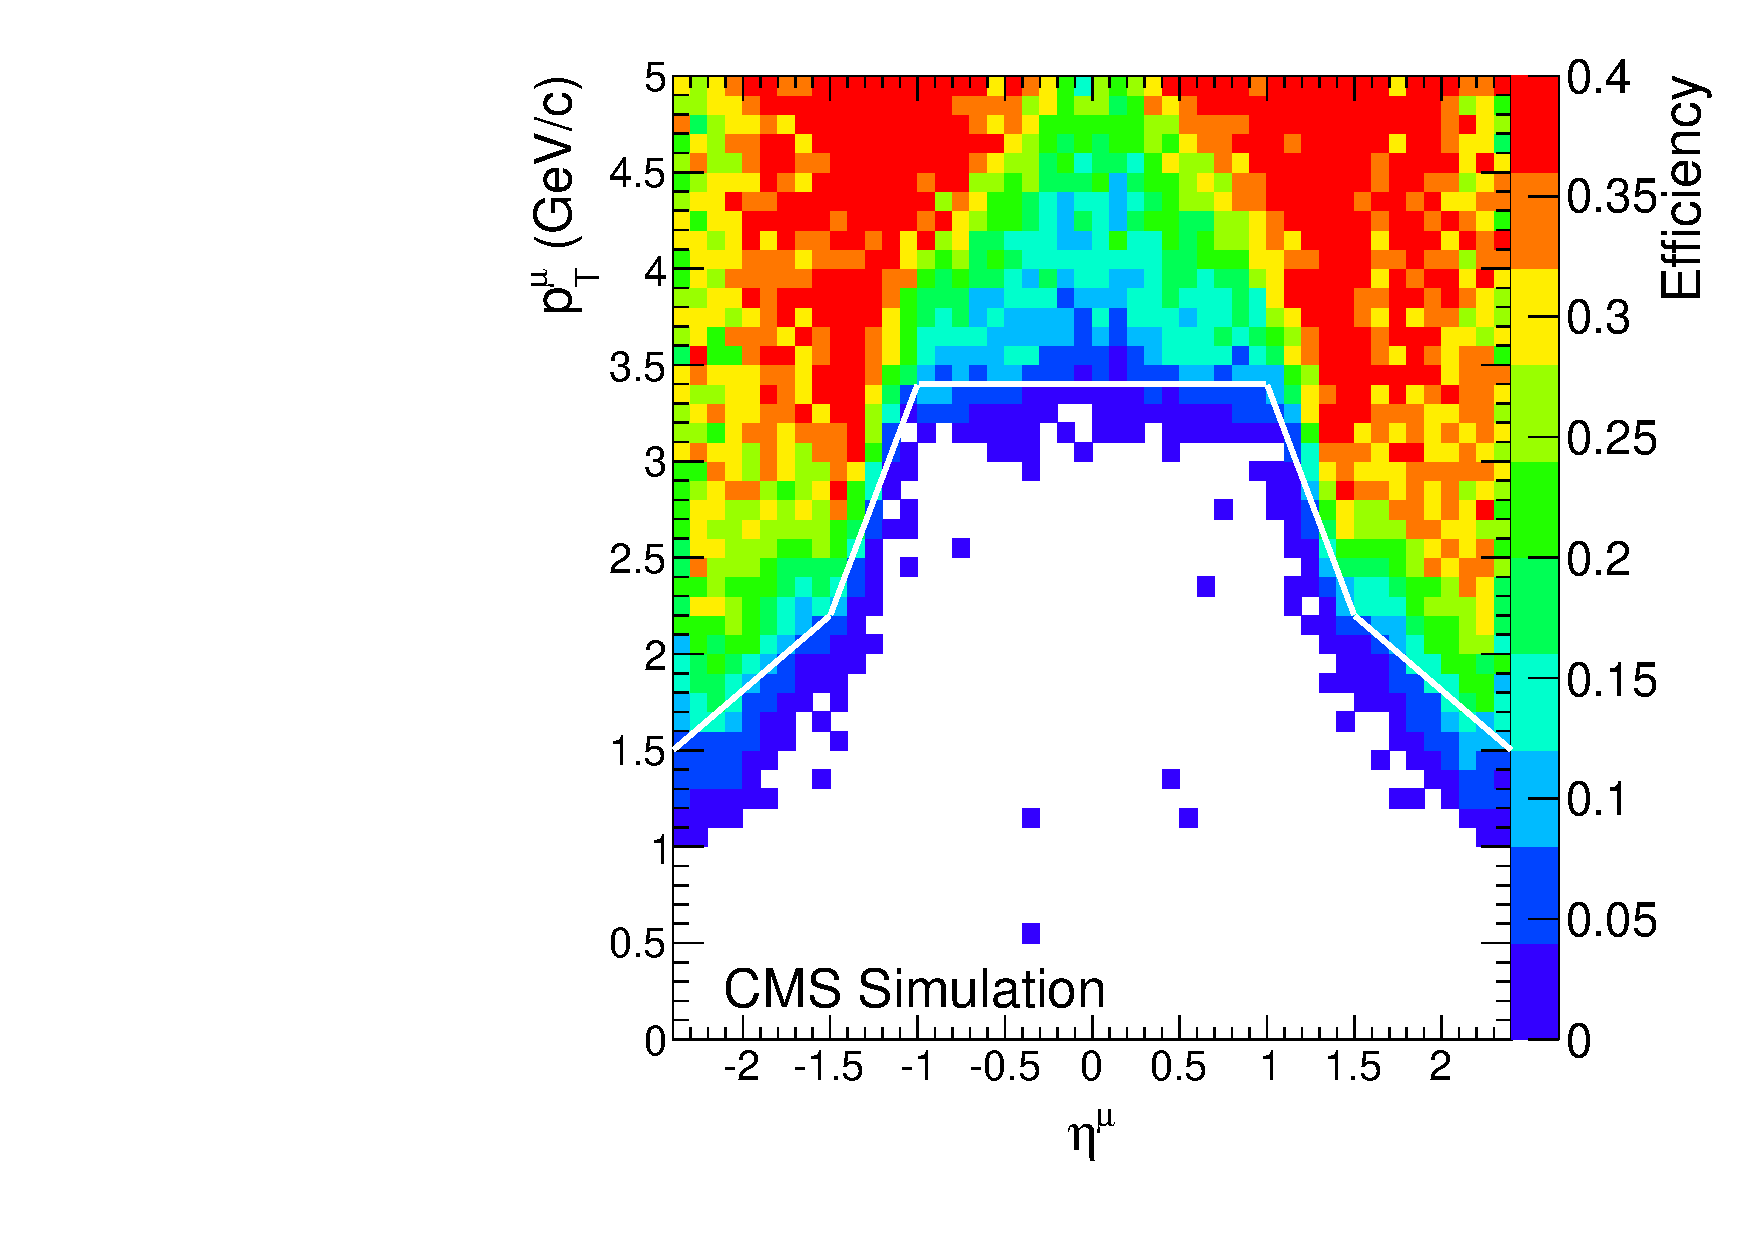
\includegraphics[width=0.5\linewidth]{chap_YInPbPbColl2010_figures/muPtEtaDoable}
  \caption{Reconstruction efficiency of global muons in the ($\eta^{\mu}$,
    $\pt^{\mu}$) space, illustrating the lower limits (white lines) of
    what is considered a detectable single muon for the analysis.}
  \label{fig:muPtEtaDoable}
\end{figure}

For the \PgUa\ analysis, where the signal-to-background ratio is less
favourable than in the \Jpsi mass range, a higher $\pt^{\mu}$ is
required than for the \Jpsi analysis,
\begin{equation}
  \label{eq:singleMuonAccUps}
    \pt^{\mu}>4\GeVc,
\end{equation}
independent of $\eta^{\mu}$.

Various additional global muon selection criteria are studied in MC
simulations. The MC distributions of the \Jpsi decay muons are in
agreement with those from data to better than 2\%, which is within the
systematic uncertainty of the data/MC efficiency ratio
(Section~\ref{sec:eff}). The transverse (longitudinal) distance of
closest approach to the measured vertex is required to be less than 3
(15)\,cm. Tracks are only kept if they have 11 or more hits in the
silicon tracker, and the $\chi^2$ per degree of freedom of the global
(inner) track fit is less than 20 (4). The $\chi^2$ probability of the
two tracks originating from a common vertex is required to be larger
than 1\%. From MC simulations we find that these criteria result in a
3.9\% loss of \PgUa\ events, respectively, given two reconstructed 
tracks associated with the double muon trigger.

\section{Signal Extraction}
\label{sec:signal-extraction}
\subsection{\texorpdfstring{\PgUa}{Upsilon(1S)} Analysis}
\label{sec:upsilon}
To extract the \PgUa\ yield, an extended unbinned maximum-likelihood
fit to the \mumu invariant mass spectrum between 7 and 14 GeV/$c^2$ is
performed, integrated over \pt, rapidity, and centrality, as shown in
the left panel of \fig{fig:ups_invmass}. The measured mass line shape
of each \PgU\ state is parametrised by a Crystal Ball function. Since
the three \PgU\ resonances partially overlap in the measured dimuon
mass spectrum, they are fitted simultaneously. Therefore, the
probability distribution function describing the signal consists of
three Crystal Ball functions. In addition to the three \PgUn\ yields,
the \PgUa\ mass is the only parameter left free, to accommodate a
possible bias in the momentum scale calibration. The mass ratios
between the states are fixed to their world average
values~\cite{Nakamura:2010zzi}, and the mass resolution is forced to
scale linearly with the resonance mass. The \PgUa\ resolution is fixed
to the value found in the simulation, 92 MeV/$c^2$. This value is
consistent with what is measured when leaving this parameter free in a
fit to the data, $(122 \pm 30) MeV/c^2$. The low-side tail parameters in
the Crystal Ball function are also fixed to the values obtained from
simulation. Finally, a second-order polynomial is chosen to describe
the background in the mass range 7--14 GeV/$c^2$. From this fit, before
accounting for acceptance and efficiencies, the measured \PgUa\ raw
yield is $86 \pm 12$. The observed suppression of the excited states
was discussed in~\cite{Chatrchyan:2011pe}. The fitted mean value is
$m_0 = (9.441\pm0.016) GeV/c^2$, which is, slightly below the PDG 
value $m_{\PgUa} = 9.460 GeV/c^2$~\cite{Nakamura:2010zzi} because
of slight momentum scale biases in the data reconstruction.

\begin{figure*}[htbp]
  \begin{center}
    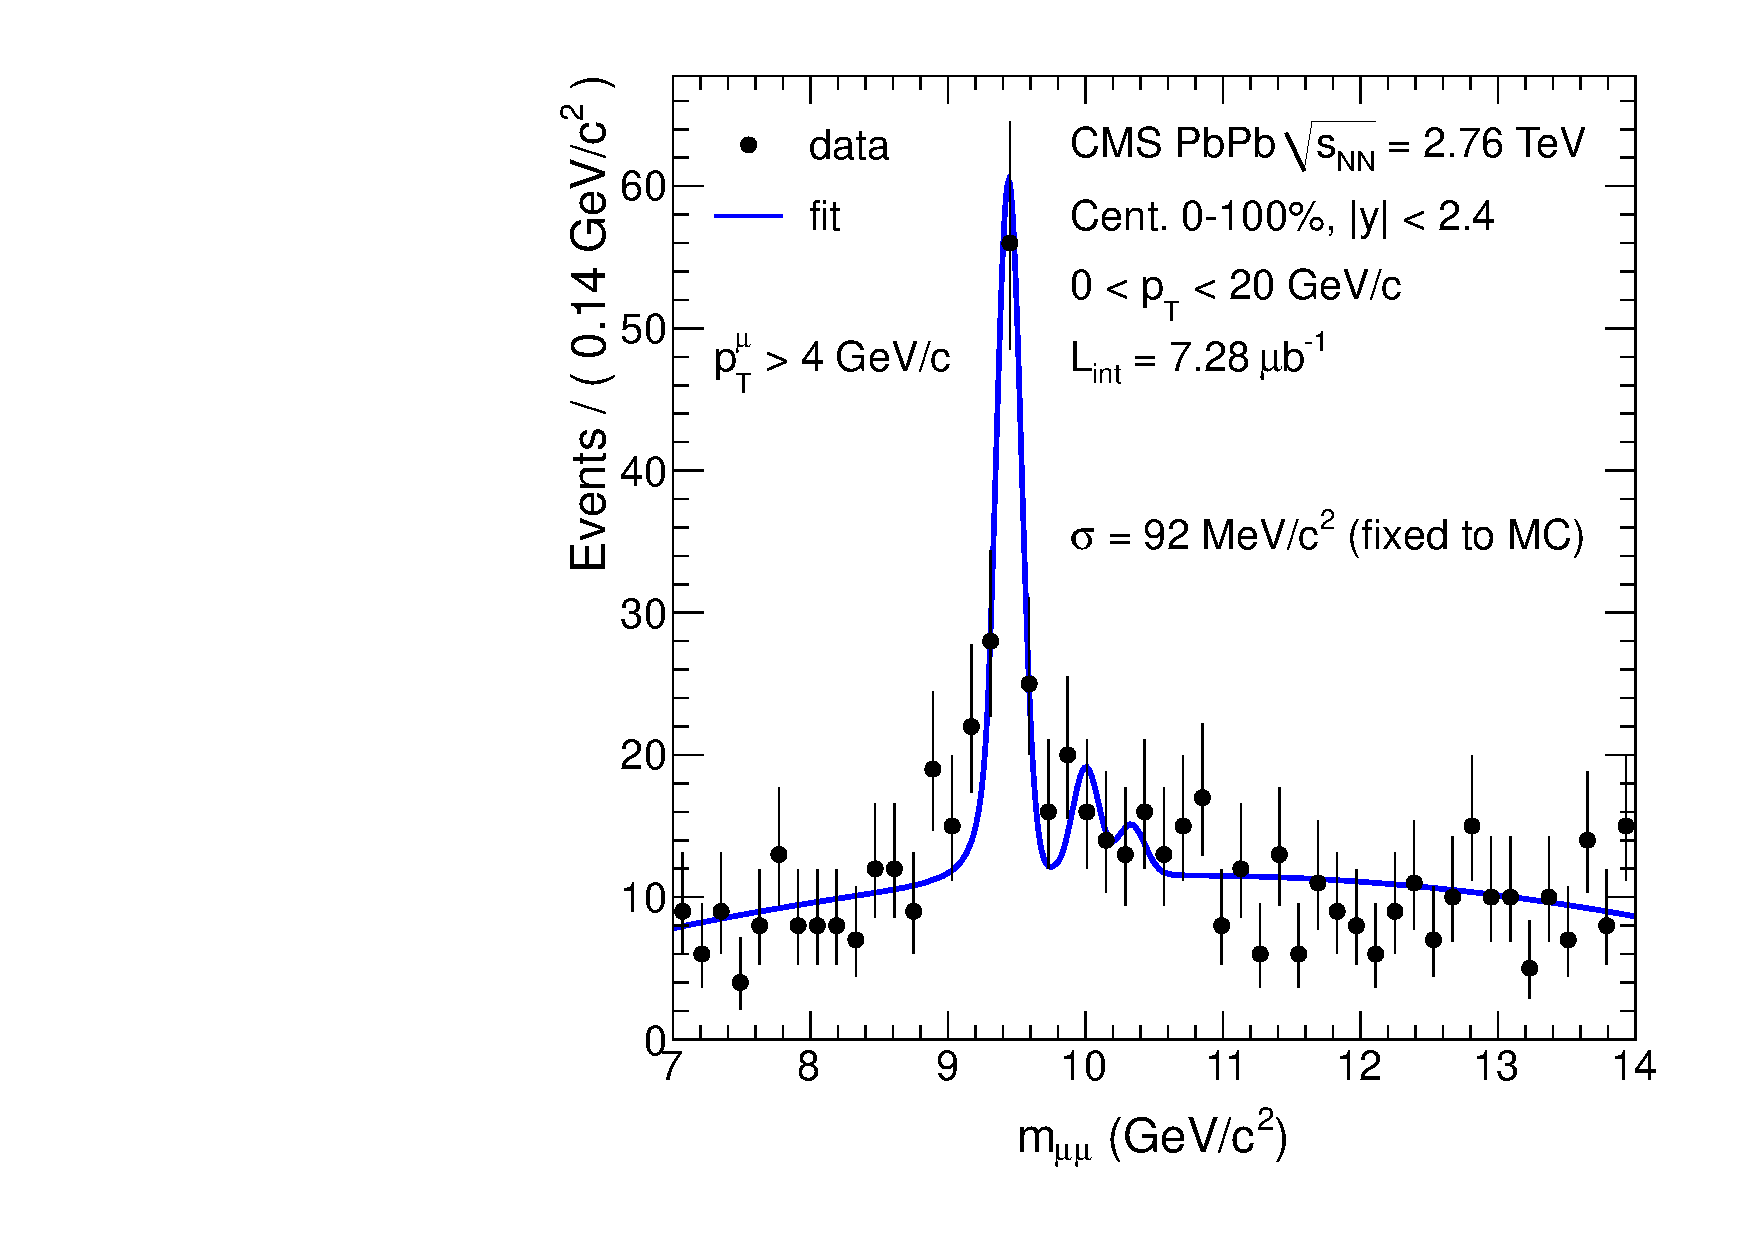
\includegraphics[width=0.45\textwidth]{chap_YInPbPbColl2010_figures/masspeak_Hi.pdf}
    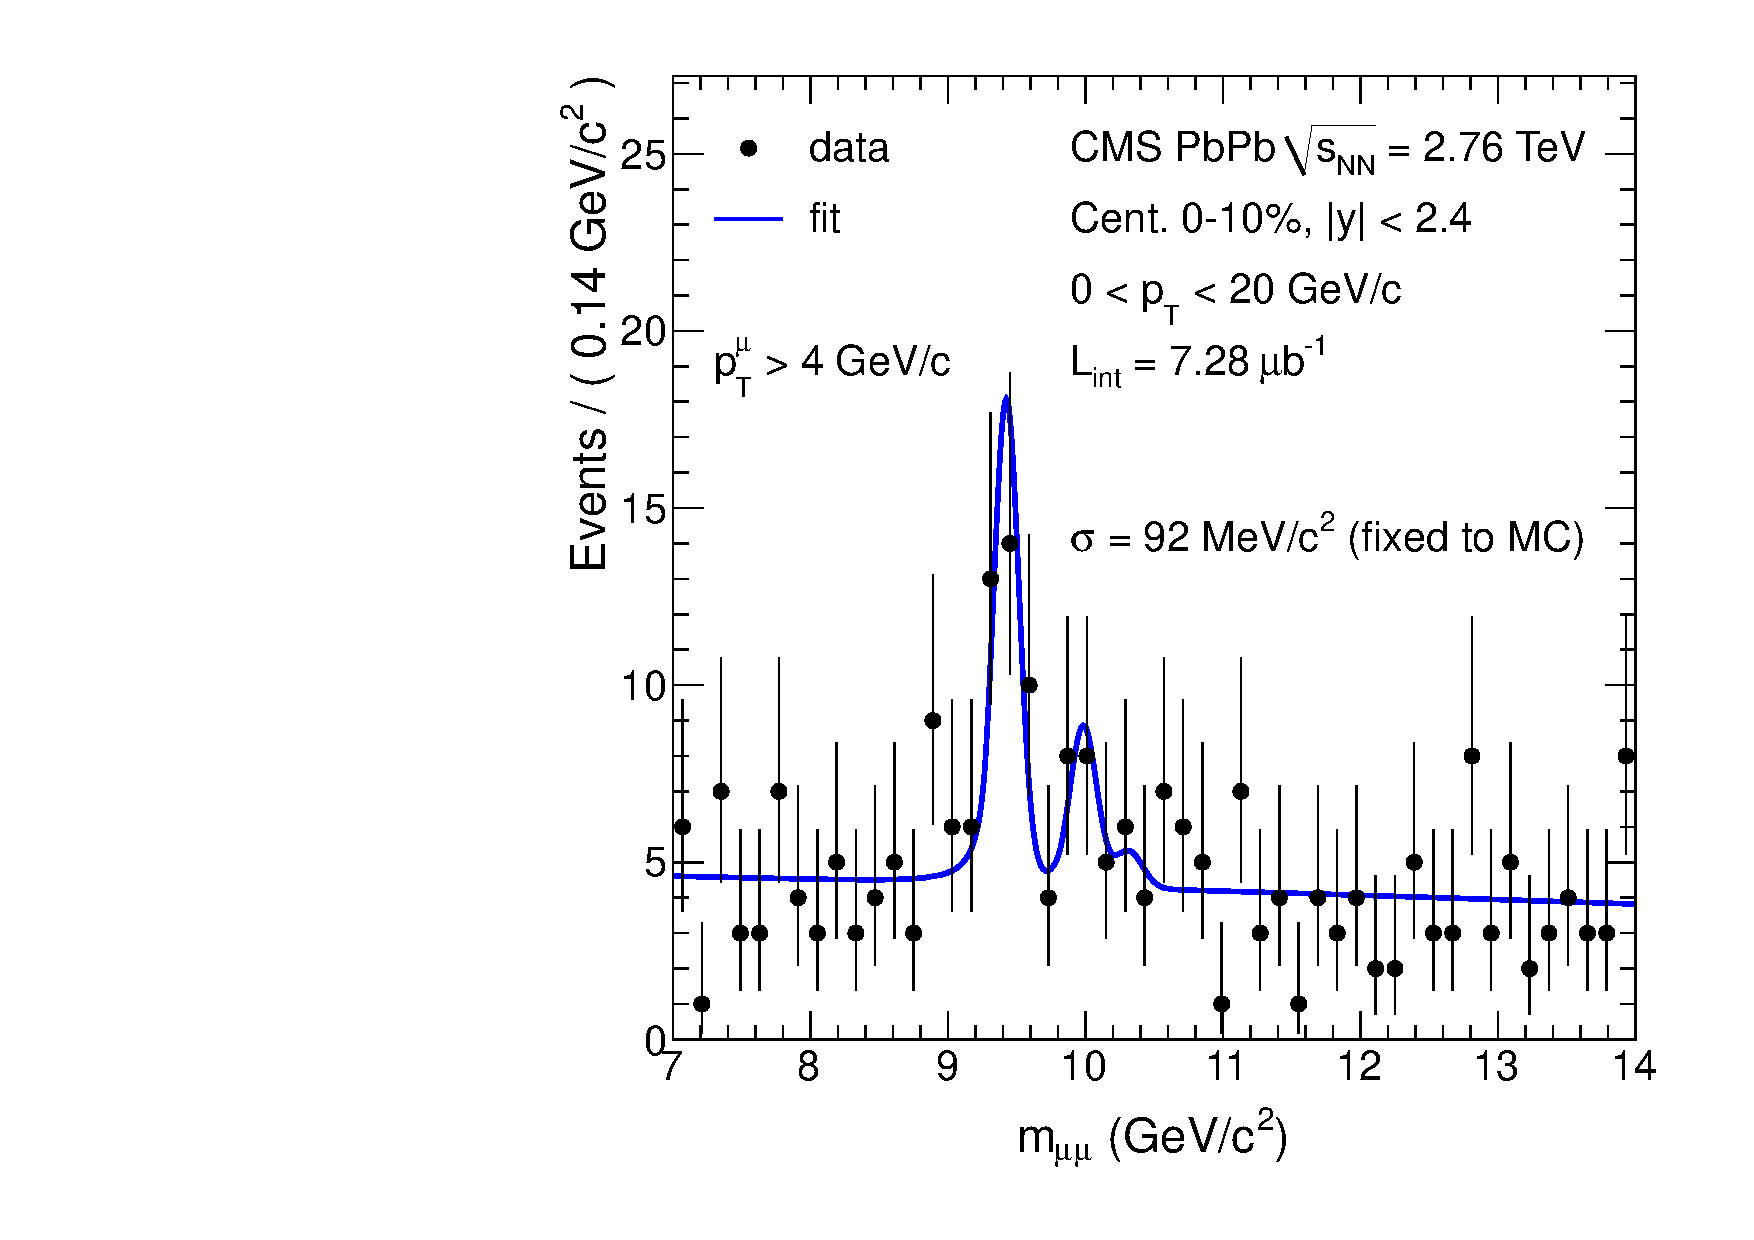
\includegraphics[width=0.45\textwidth]{chap_YInPbPbColl2010_figures/masspeak_Hi_cntr0-10.pdf}
    \caption{Invariant-mass spectrum of \mumu pairs (black circles)
      with $\pt<20\GeV/c$ and $|y|<2.4$, for muons above 4\GeVc,
      integrated over centrality (left) and for the 0--10\% centrality
      bin (right).}
    \label{fig:ups_invmass}
  \end{center}
\end{figure*}

The data are binned in \pt and rapidity of the \mumu pairs, as well as
in bins of the event centrality (0--10\%, 10--20\%, and
20--100\%). The bins in rapidity are $|y|<1.2$ and $1.2<|y|<2.4$. In
contrast to the \Jpsi case, CMS has acceptance for \PgU\ down to
\mbox{$\pt = 0\GeVc$} over the full rapidity range. The \pt bins in
this analysis are $0<\pt<6.5\GeVc$, $6.5<\pt<10\GeVc$, and
$10<\pt<20\GeVc$. There are only two events with a \mumu pair in the
\PgU\ mass region and $\pt > 20\GeVc$. The invariant-mass distribution
for the centrality bin 0--10\% is illustrated in the right panel of
\fig{fig:ups_invmass}. The raw yields of \PgUa are tabulated
in \tab{tab:upsilonyields} of Appendix~\ref{app:datatables}.

The systematic uncertainties are computed by varying the line shape in
the following ways: (i) the Crystal Ball function tail parameters are
varied randomly according to their covariance matrix and within
conservative values covering imperfect knowledge of the amount of
detector material and final-state radiation in the underlying process;
(ii) the width is varied by $\pm 5\MeV/c^2$, a value motivated by the
current understanding of the detector performance (eg., the dimuon
mass resolution, accurately measured at the \Jpsi mass, is identical
in \pp and \PbPb collisions); (iii) the background shape is changed
from quadratic to linear, and the mass range of the fit is varied from
6--15 to 8--12 $\GeV/c^2$; the observed RMS of the results in each category
is taken as the systematic uncertainty. The quadratic sum of these
three systematic uncertainties is dominated by the variation of the
resolution of the mass fit, and is of the order of 10\%, reaching 13\%
for the 0--10\% centrality bin. As was the case for the \Jpsi
selection, a simple counting of the yield in the signal region after
the subtraction of the same-sign spectrum leads to consistent results.


\section{Acceptance and Efficiency}
\label{sec:acceff}
\subsection{Acceptance}
\label{sec:acc}
The dimuon acceptance, $A$, is defined as the fraction of \mumu pairs
for which both muons are declared detectable in the CMS detector with
respect to all muon pairs produced in $|y|<2.4$,
\begin{equation}
  \label{eq:acc}
    A(\pt,y;\lambda_{\theta}) = \frac{N^{\Pgm\Pgm}_{\text{detectable}}(\pt,y;\lambda_{\theta})}{N^{\Pgm\Pgm}_{\text{generated}}(\pt,y;\lambda_{\theta})},
\end{equation}
where:
\begin{itemize}
\item N$^{\Pgm\Pgm}_{\text{detectable}}$ is the number of generated
  events in a given quarkonium (\pt, $y$) bin in the MC simulation,
  for which both muons are detectable according to the selections
  defined in Eqs.~\eqref{eq:singleMuonAcc}
  and~\eqref{eq:singleMuonAccUps};
\item N$^{\Pgm\Pgm}_{\text{generated}}$ is the number of all \mumu pairs
  generated within the considered (\pt, $y$) bin.
\end{itemize}
The acceptance depends on the \pt and $y$ of the \mumu pair, and the
polarization parameter $\lambda_{\theta}$. Different polarizations of
the \Jpsi and \PgUa\ will cause different single-muon angular
distributions in the laboratory frame and, hence, different
probabilities for the muons to fall inside the CMS detector
acceptance. Since the quarkonium polarization has not been measured in
heavy-ion or \pp collisions at \sqrtsnn = 2.76\TeV, the prompt \Jpsi
and \PgUa\ results are quoted for the unpolarized scenario only. For
non-prompt \Jpsi the results are reported for the polarization
predicted by EVTGEN. The impact of the polarization on the
acceptance is studied for the most extreme polarization scenarios in
the Collins--Soper and helicity frames. For fully longitudinal
(transverse) polarized \Jpsi in the Collins--Soper frame, the effect
is found to be at most $-20\%$ (6\%). In the helicity frame, the
effects are at most 40\% and $-20\%$ for the two scenarios. For \PgUa\
the polarization effects range between $-20\%$ for longitudinal
polarization in the Collins--Soper frame to 40\% for transverse
polarization in the helicity frame.
The acceptance is calculated using the MC sample described in
Section~\ref{sec:event-sel}. The \pt and rapidity dependencies of the
\Jpsi and \PgUa\ acceptances are shown in \fig{fig:acceptance}.

\begin{figure*}[htbp]
  \centering
  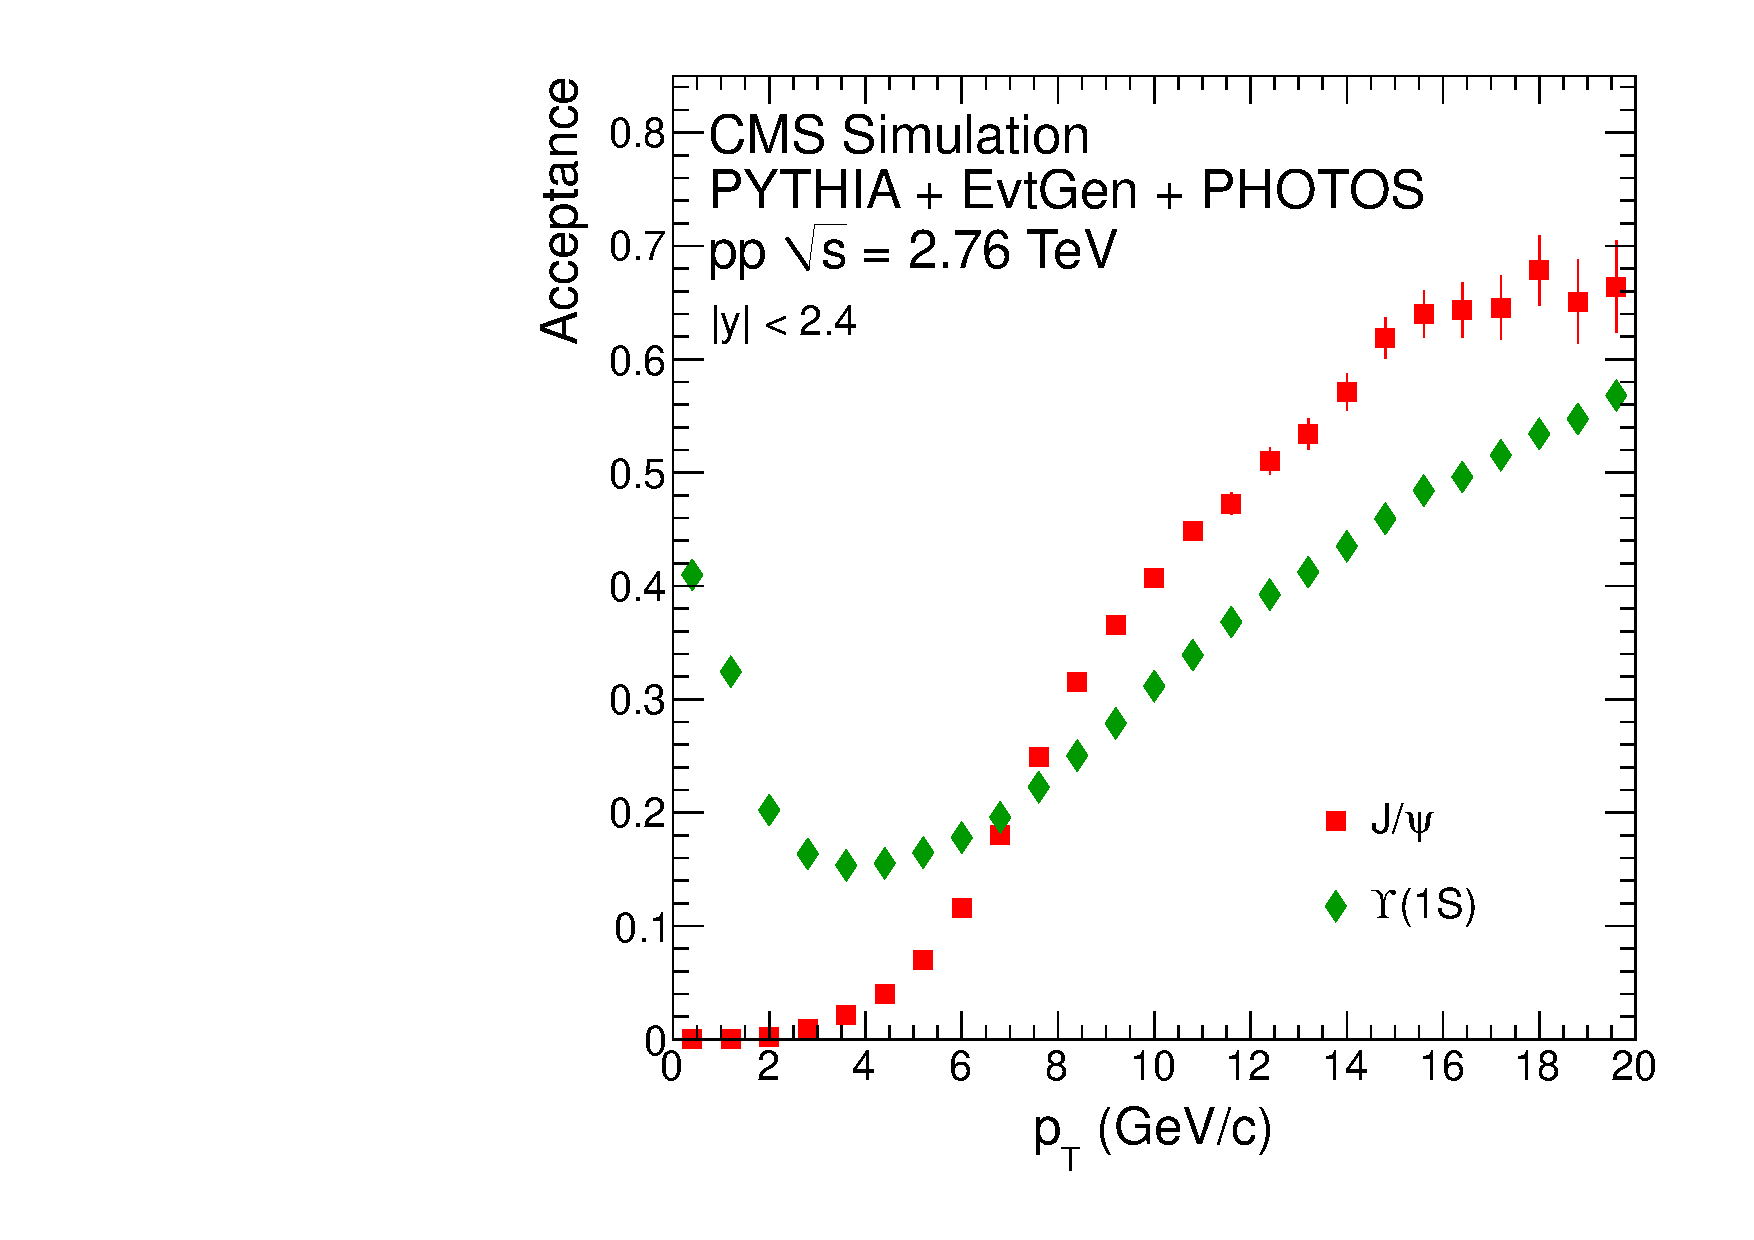
\includegraphics[width=0.45\linewidth]{chap_YInPbPbColl2010_figures/acc_pt_promptJpsi}
  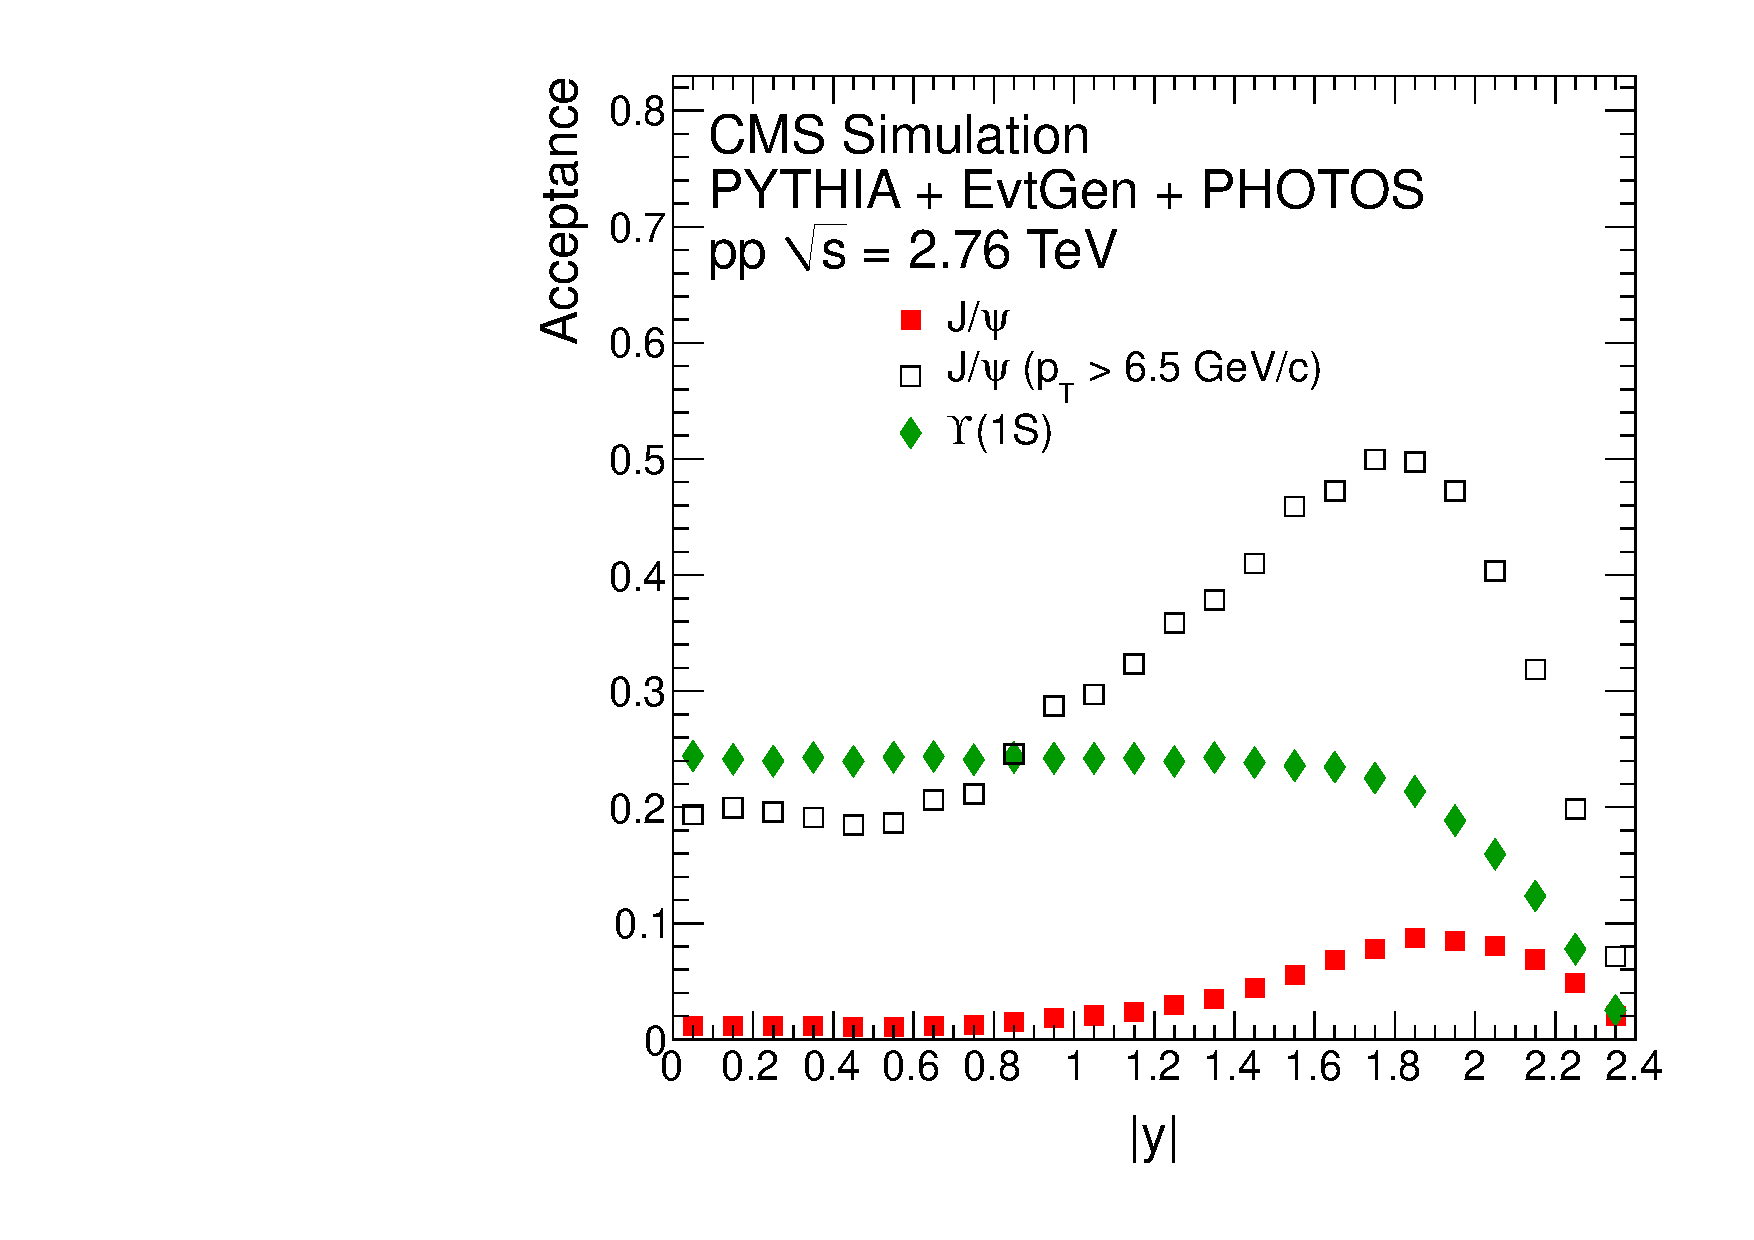
\includegraphics[width=0.45\linewidth]{chap_YInPbPbColl2010_figures/acc_y_promptJpsi}
  \caption{Dimuon acceptance as a function of \pt (left) and $|y|$
    (right) for \Jpsi (red squares) and \PgUa\ (green diamonds). Also
    shown in the right panel is the acceptance for \Jpsi with
    $\pt>6.5\GeVc$ (open black squares). The error bars represent the
    statistical uncertainties only.}
  \label{fig:acceptance}
\end{figure*}
Since the acceptance is a function of both \pt and $y$, uncertainties
in the predicted distributions for these variables can lead to a
systematic uncertainty in the average acceptance over a \pt or $y$
bin.  To estimate these uncertainties, the shapes of the generated MC
\pt and $|y|$ distributions are varied by applying a weight that
increases linearly from 0.7 to 1.3 over the range $0<|y|<2.4$ and
$0<\pt<30\GeVc$ (20\GeVc) for \Jpsi (\PgUa).  The RMS of the resulting
changes in the acceptance for each \pt and $y$ bin are summed in
quadrature to compute the overall systematic uncertainty from this
source.  The largest relative systematic uncertainties obtained are
4.2\%, 3.2\%, and 2.8\% for the prompt \Jpsi, non-prompt \Jpsi, and
\PgUa\ acceptances, respectively.

\subsection{Efficiency}
\label{sec:eff}

The trigger, reconstruction, and selection efficiencies of \mumu pairs
are evaluated using simulated MC signal events embedded in simulated
\PbPb events, as described in Section~\ref{sec:event-sel}. The overall
efficiency is calculated, in each analysis bin, as the fraction of
generated events (passing the single muon phase space cuts) where both
muons are reconstructed, fulfil the quality selection criteria and
pass the trigger requirements. In the embedded sample, the signal over
background ratio is by construction higher than in data, so the
background contribution underneath the resonance peak is negligible
and the signal is extracted by simply counting the \mumu pairs in the
quarkonium mass region. The counting method is crosschecked by using
exactly the same fitting procedure as if the MC events were collision
data. Only muons in the kinematic region defined by
Eqs.~\eqref{eq:singleMuonAcc} and~\eqref{eq:singleMuonAccUps} are
considered.
In \fig{fig:eff}, the efficiencies are shown as a function of the
\mumu pair \pt, $y$, and the event centrality, for each signal: red
squares for prompt \Jpsi, orange stars for non-prompt \Jpsi, and green
diamonds for \PgUa. The efficiency of non-prompt \Jpsi is lower than that 
of prompt \Jpsi, reaching about 35\% for $\pt > 12\GeVc$. 
The prompt \Jpsi efficiency increases with \pt until reaching a plateau 
slightly above 50\% at \pt
of about 12\GeVc, while the \PgUa\ efficiency is $\sim\!55\%$,
independent of \pt. The efficiencies decrease slowly as a function of
centrality because of the increasing occupancy in the silicon tracker;
the relative difference between peripheral and central collisions is
17\% for \Jpsi and 10\% for \PgUa. The integrated efficiency values
are 38.3\%, 29.2\%, and 54.5\% for the prompt \Jpsi, non-prompt \Jpsi
(both with $6.5<\pt<30\GeVc$, $|y|<2.4$, and 0--100\% centrality), and
\PgUa\ (with $0<\pt<20\GeVc$, $|y|<2.4$, and 0--100\% centrality),
respectively.
\begin{figure}[htbp]
  \centering
  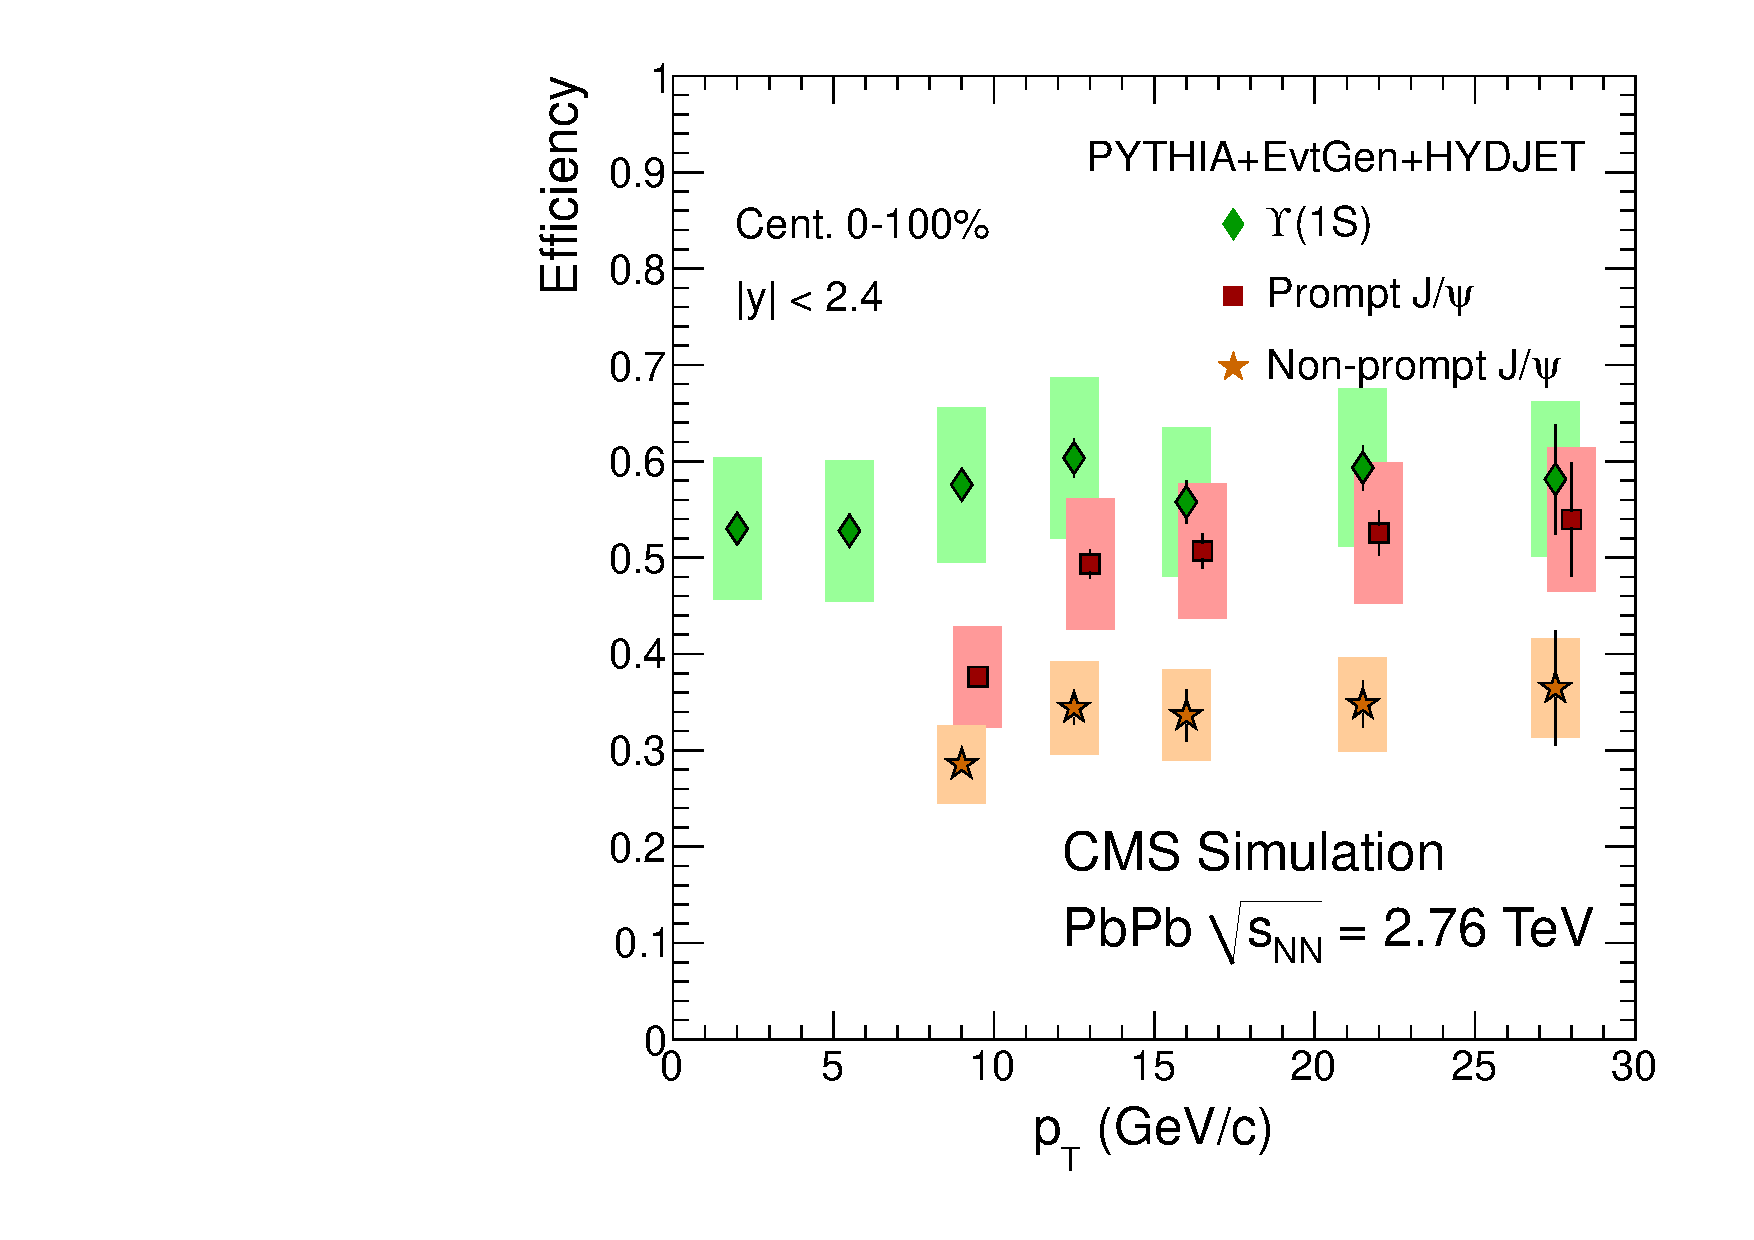
\includegraphics[width=0.45\linewidth]{chap_YInPbPbColl2010_figures/QuarkoniaEff_pt}
  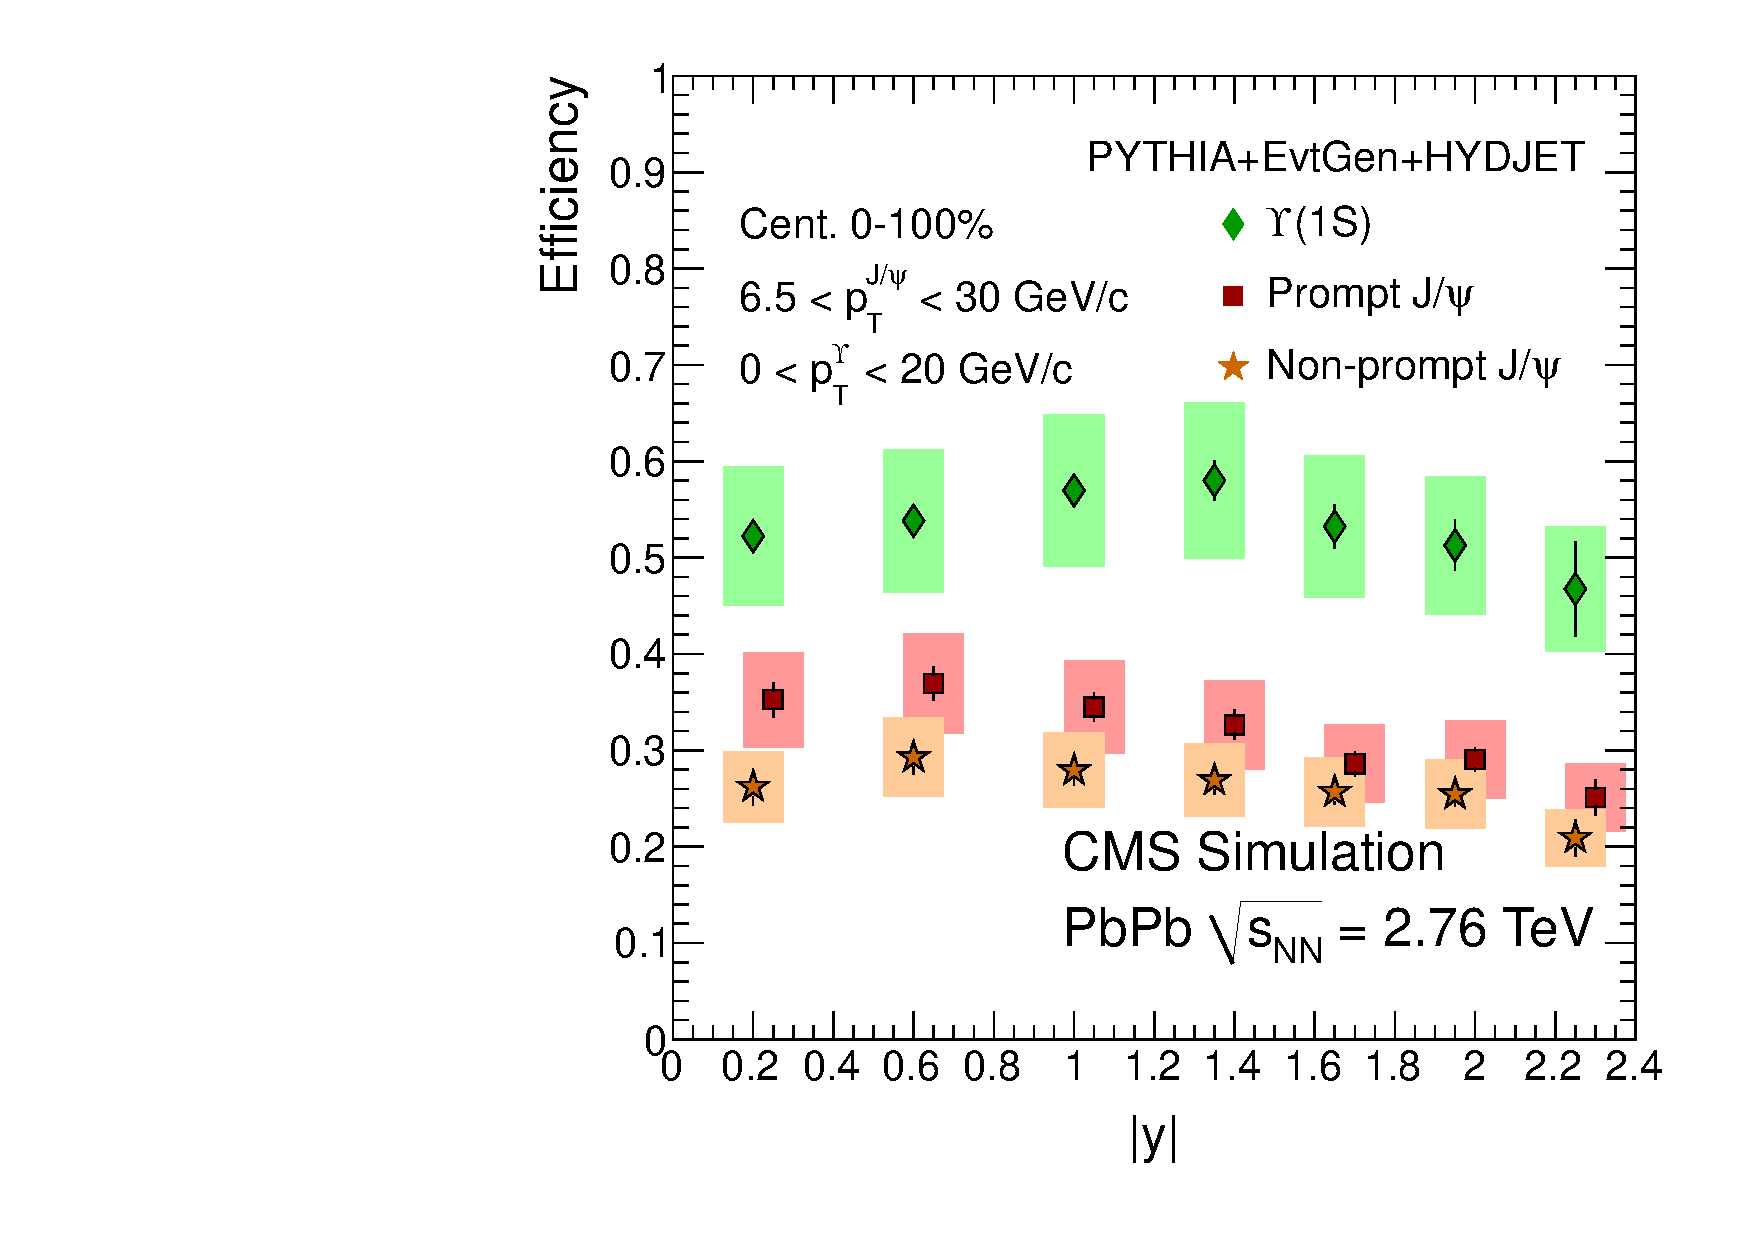
\includegraphics[width=0.45\linewidth]{chap_YInPbPbColl2010_figures/QuarkoniaEff_y}\\
  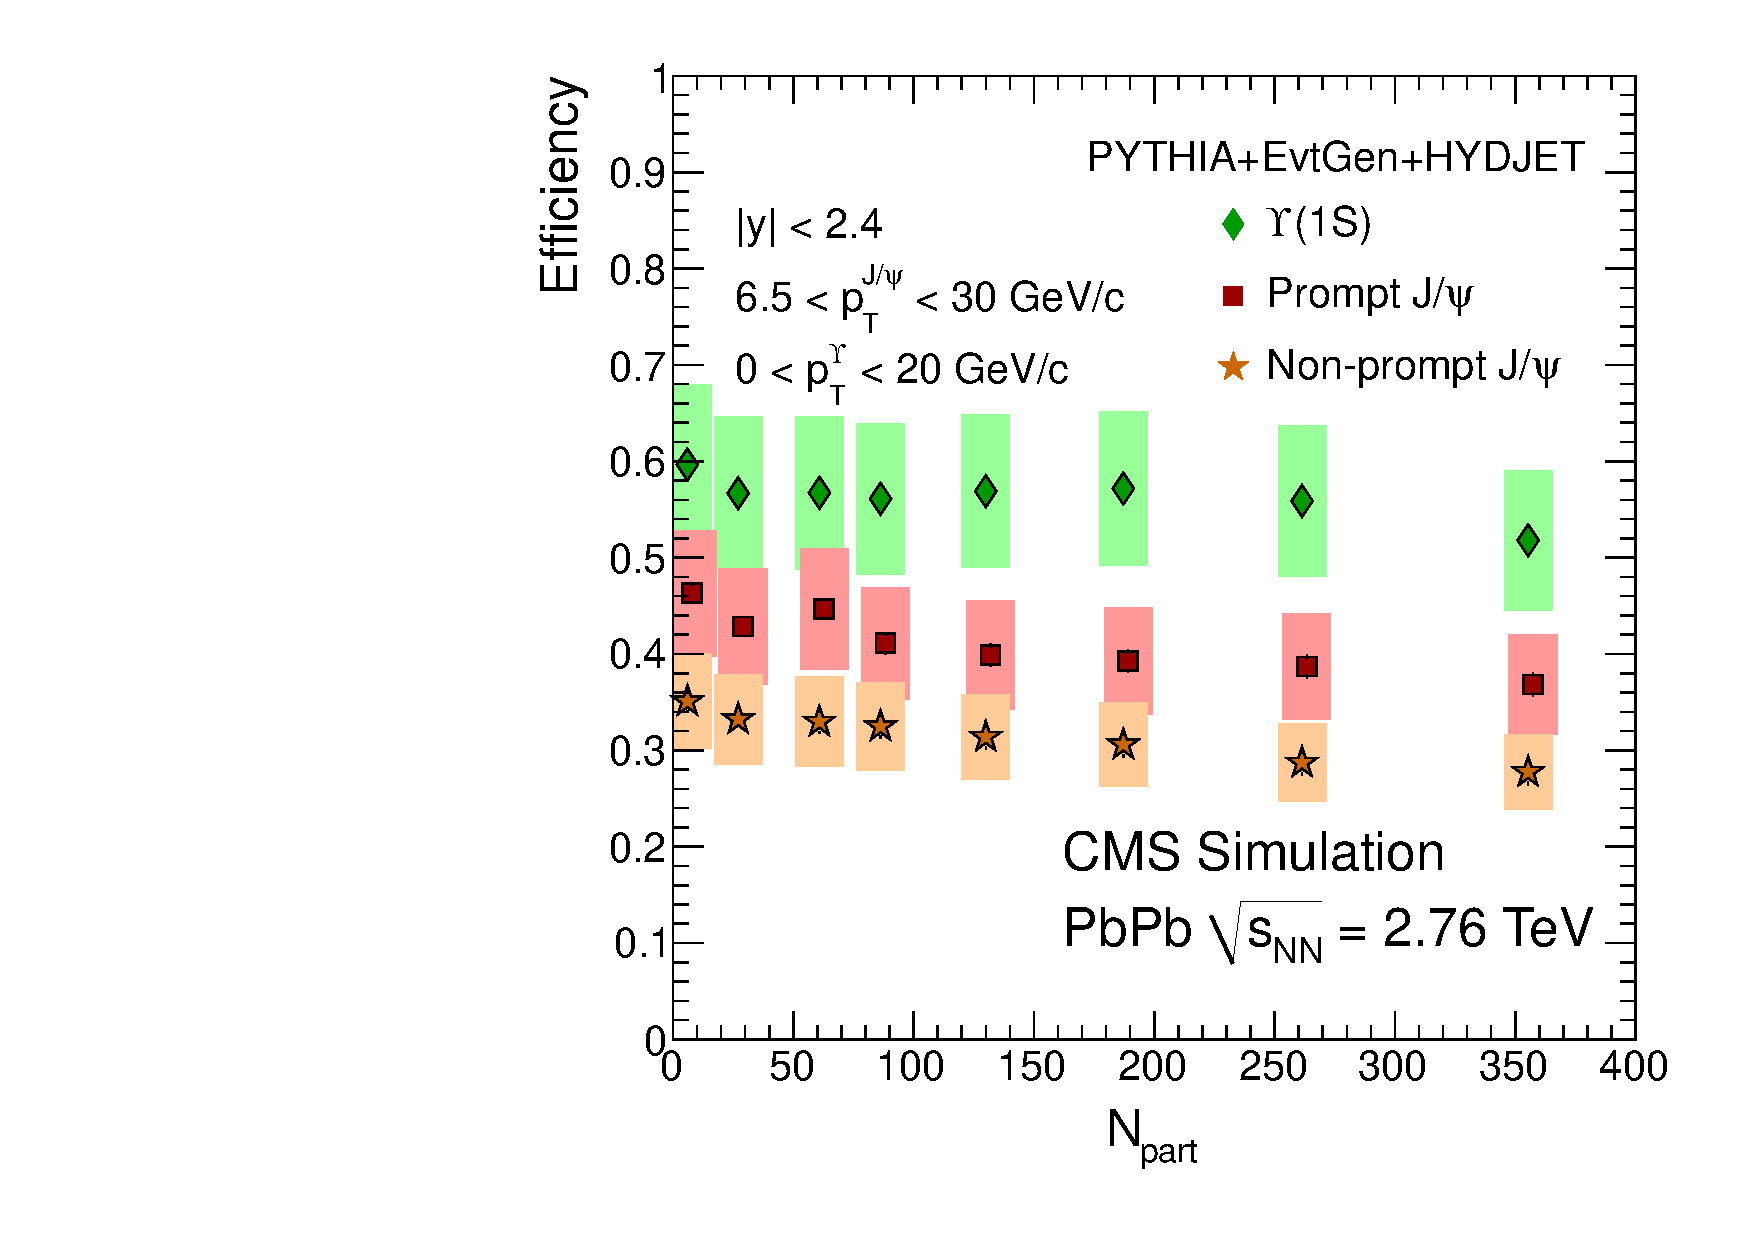
\includegraphics[width=0.45\linewidth]{chap_YInPbPbColl2010_figures/QuarkoniaEff_cent}
  \caption{Combined trigger, reconstruction, and selection
    efficiencies as a function of quarkonium \pt and $|y|$, and event
    centrality, for each signal: red squares and orange stars for
    prompt and non-prompt \Jpsi, respectively, and green diamonds for
    \PgUa. For better visibility, the prompt \Jpsi points are shifted
    by $\Delta \pt = 0.5\GeVc$, $\Delta y=0.05$, and $\Delta \npart =
    2$. Statistical (systematic) uncertainties are shown as bars
    (boxes). The systematic uncertainties are the quadratic sum of the
    uncertainty on the kinematic distributions and the MC validation
    uncertainty.}
  \label{fig:eff}
\end{figure}

The systematic uncertainty on the final corrections due to the
kinematic distributions is estimated by a $\pm30\%$ variation of the
slopes of the generated \pt and rapidity shapes, similar to the
acceptance variation described in the previous section. The systematic
uncertainties are in the ranges 1.8--3.4\%, 2.2--4.2\%, and 1.4--2.7\%
for prompt \Jpsi, non-prompt \Jpsi, and \PgUa, respectively, including
the statistical precision of the MC samples.
The individual components of the MC efficiency are crosschecked using
muons from \Jpsi decays in simulated and collision data with a
technique called \emph{tag-and-probe}, similar to the one used for the
corresponding \pp measurement~\cite{Khachatryan:2010yr}.

\section{The pp Baseline Measurement}
\label{sec:ppRef}
A \pp run at \sqrts = 2.76\TeV was taken in March 2011. The integrated
luminosity was 231 nb$^{-1}$, with an associated uncertainty of 6\%. For
hard-scattering processes, the integrated luminosity of the \pp sample
is comparable to that of the \PbPb sample (\mbox{$7.28 \mu\,b^{-1} \cdot
208^2 \approx 315 nb^{-1}$}).

Given the higher instantaneous luminosity, the 
trigger required
slightly higher quality muons in the \pp run than in the \PbPb
run. The offline event selection is the same as in the \PbPb analysis,
only slightly relaxed for the HF coincidence requirement: instead of
three towers, only one tower with at least 3 GeV deposited is required
in the \pp case. The same reconstruction algorithm, i.e. the one
optimized for the heavy-ion environment, is used for both \pp and
\PbPb data. The products of the trigger, reconstruction, and selection
efficiencies determined in \pp MC simulations are 42.5\%, 34.5\%, and
55.1\% for the prompt \Jpsi, non-prompt \Jpsi (both with
$6.5<\pt<30\GeVc$, $|y|<2.4$), and \PgUa\ (with $0<\pt<20\GeVc$,
$|y|<2.4$), respectively.
The quarkonium signals in \pp collisions are extracted following the
same methods as in \PbPb collisions.

The invariant-mass spectrum of \mumu pairs in the $\PgU$ region from
\pp collisions is shown in \fig{fig:ups_pp}. The same procedure as the
one described for the \PbPb analysis is used. The number of $\PgUa$
mesons with $|y|<2.4$ and $0<\pt<20\,\GeV/c$ is $101\pm12$. The fit
result of the excited states is discussed in~\cite{Chatrchyan:2011pe}.

\begin{figure}[hbtp]
  \begin{center}
  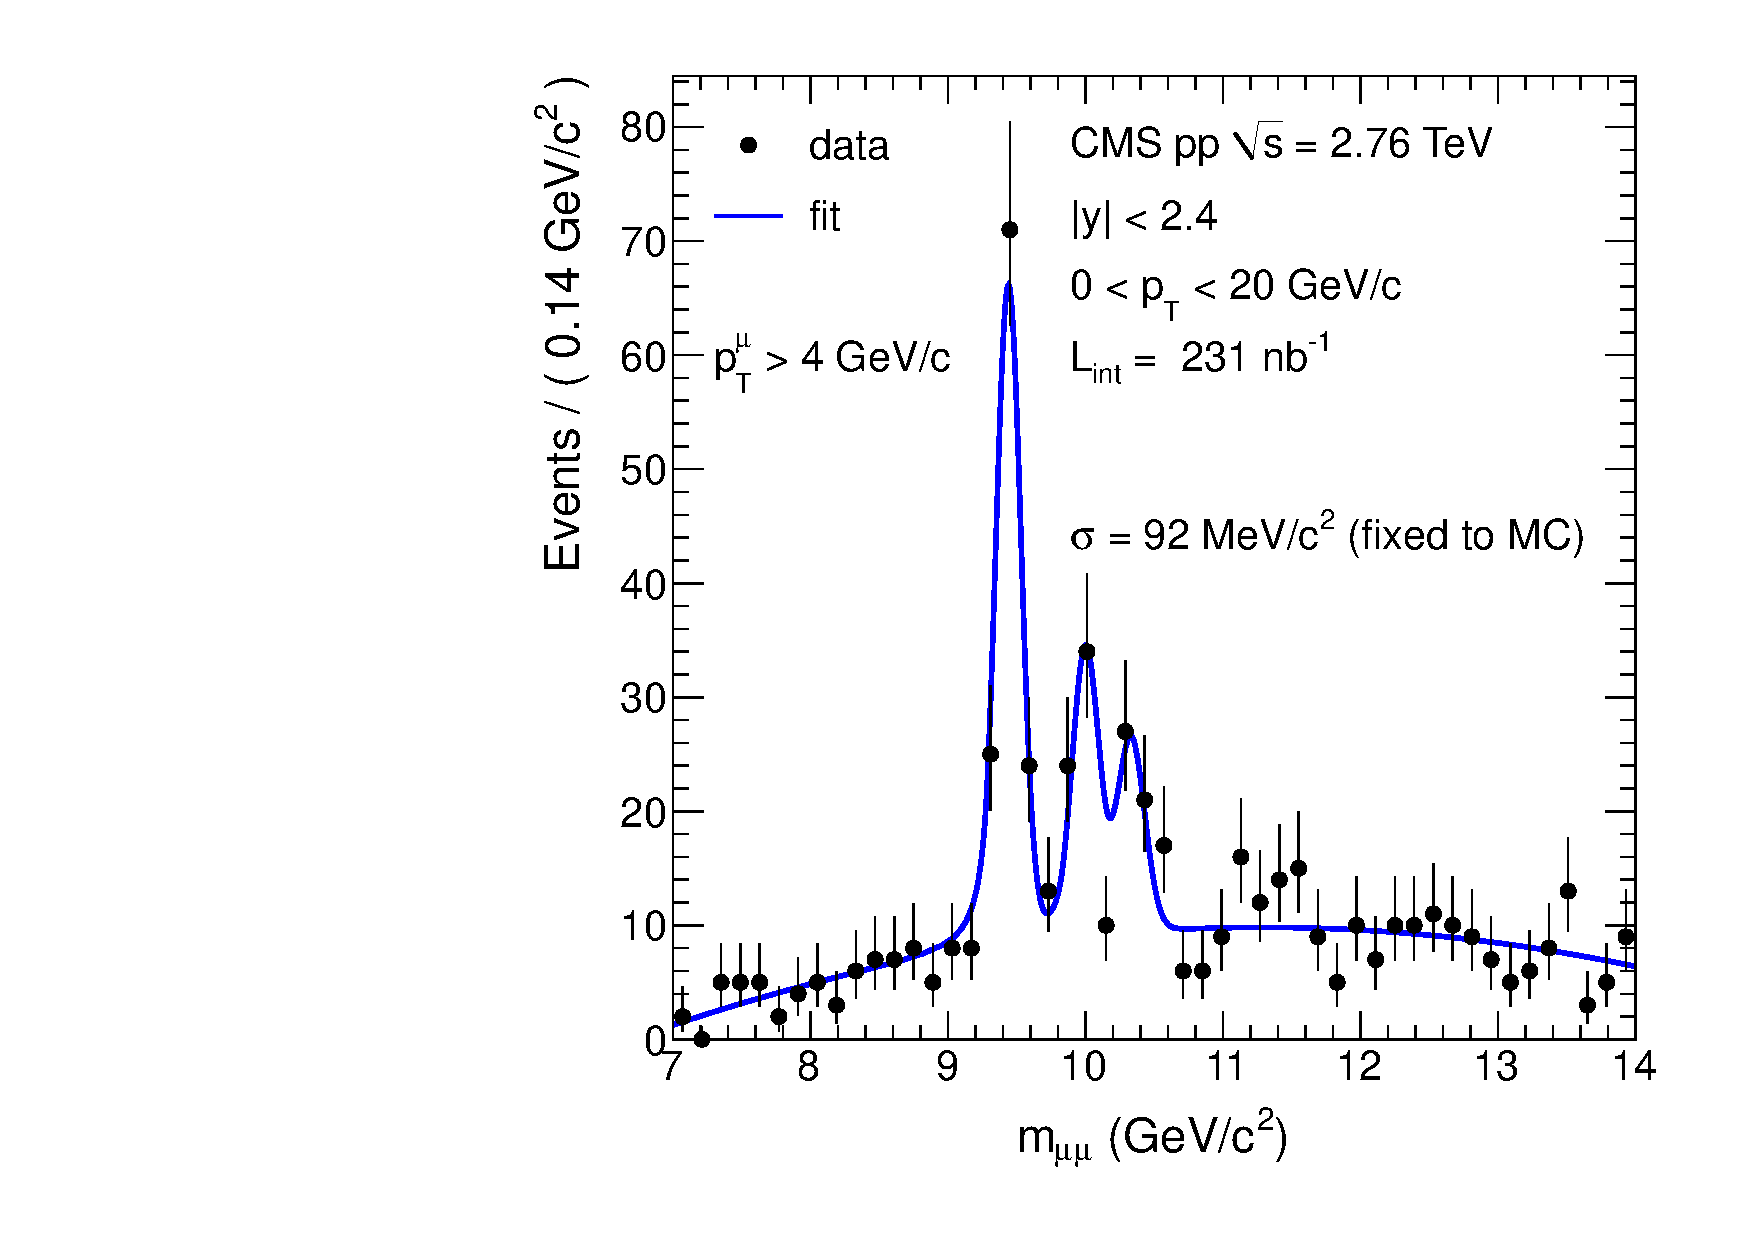
\includegraphics[width=0.5\linewidth]{chap_YInPbPbColl2010_figures/masspeak_pp_HIrereco}
  \caption{The \pp dimuon invariant-mass distribution in the range
    $\pt<20 \GeVc$ for $|y|<2.4$ and the result of the fit to the
    $\PgU$ resonances.}
  \label{fig:ups_pp}
  \end{center}
\end{figure}

For the measurement of the nuclear modification factors, in which the
ratio of \PbPb to \pp results is computed, most of the reconstruction
systematic uncertainties cancel out because the same algorithm is
used. However, the following factors must be accounted for:

\begin{enumerate}
\item The luminosity uncertainty. This is a global systematic
  uncertainty of 6\% that allows all measured nuclear modification
  factors to change by a common scale-factor. Since the \PbPb yield is
  normalized by the number of minimum-bias events, which has a
  negligible uncertainty, no systematic uncertainty on the \PbPb
  luminosity has to be considered.
\item The uncertainty on \taa. For results integrated over centrality,
  this is a global systematic uncertainty of 5.7\%, based on the
  Glauber model employed. For results as a function of centrality, the
  uncertainty varies between a minimum of 4.3\% in the most central
  bin and a maximum of 15\% in the most peripheral
  bin~\cite{Chatrchyan:2011sx}.
\item The systematic uncertainty associated with the trigger
  efficiency. The ratios between the \emph{tag-and-probe} efficiencies
  obtained in \pp and \PbPb are the same in data and MC events, within
  the statistical accuracy of the data (1\% for the single-muon
  efficiency).  Twice this value (2\%) is assigned as the uncertainty
  on the difference of the trigger efficiencies of \mumu pairs in
  \PbPb and \pp collisions.
\item The tracking efficiency uncertainty due to different charged
  particle multiplicities in \pp and \PbPb collisions.  The ratios
  between the \emph{tag-and-probe} efficiencies obtained in \pp and
  central \PbPb events are the same in data and MC events, within the
  statistical accuracy of the data (6.8\% for the single-muon
  efficiency).  This value is propagated as the tracking systematic
  uncertainty in all the ratios of \PbPb to \pp data.
\end{enumerate}

\section{Results}
\label{sec:results}

The double-differential quarkonium cross sections in \PbPb collisions
are reported in the form
\begin{equation}
  \label{eq:xsection}
    \frac{1}{\taa} \cdot
    \frac{\mathrm{d}^2N}{\mathrm{d}y\,\mathrm{d}\pt} = \frac{1}{\taa\, N_{\text{MB}}} \cdot \frac{1}{\Delta y\, \Delta \pt} \cdot \frac{N_{\QQbar}}{A\, \varepsilon},
\end{equation}
while in \pp collisions they are calculated as
\begin{equation}
  \label{eq:xsection_pp}
    \frac{d^2\sigma}{\mathrm{d}y\,\mathrm{d}\pt} = \frac{1}{L_{\pp}} \cdot \frac{1}{\Delta y\, \Delta \pt} \cdot \frac{N_{\QQbar}}{A\, \varepsilon},
\end{equation}
where:
\begin{itemize}
\item $N_{\QQbar}$ is the number of measured \PgUa\ in the \mumu decay channel;
\item $N_{\text{MB}}$ is the number of minimum-bias events sampled by
  the event selection; when binned in centrality, only the fraction of
  minimum-bias events in that centrality bin is considered;
\item $A$ is the geometric acceptance, which depends on the \pt and $y$
  of the quarkonium state;
\item $\varepsilon$ is the combined trigger and reconstruction
  efficiency, which depends on the \pt and $y$ of the quarkonium state
  and on the centrality of the collision;
\item $\Delta y$ and $\Delta \pt$ are the bin widths in rapidity and
  \pt, respectively;
\item \taa is the nuclear overlap function, which depends on the
  collision centrality;
\item $L_{\pp} = (231\pm14) \rm nb^{-1}$ is the integrated luminosity of
  the \pp data set.
\end{itemize}

Following \eq{eq:xsection}, the uncorrected yields of \PgUa, measured in \PbPb collisions
are corrected for acceptance and efficiency (reported in
Figs.~\ref{fig:acceptance} and \ref{fig:eff}), and converted into
yields divided by the nuclear overlap function \taa. These quantities
can be directly compared to cross sections in \pp collisions measured
from the raw yields according to \eq{eq:xsection_pp}. The rapidity and
centrality-dependent results are presented integrated over \pt. All
results are presented for the unpolarized scenario and are tabulated
in Tables~\ref{tab:inclxsec}--\ref{tab:upsilonxsectpp} of
Appendix~\ref{app:datatables}.

The systematic uncertainties detailed in the previous sections are
summarized in Tables~\ref{tab:syst_PbPb} and~\ref{tab:syst_pp}. The
relative uncertainties for all terms appearing in
Eqs.~(\ref{eq:xsection}) and~(\ref{eq:xsection_pp}) are added in
quadrature, leading to a total of 15--21\% on the corrected
yields. For results plotted as a function of \pt or rapidity, the
systematic uncertainty on \taa enters as a global uncertainty on the
scale and is not included in the systematic uncertainties of the
yields. As a function of centrality, the uncertainty on \taa varies
point-to-point and is included in the systematic uncertainties of the
yields.

\begin{table}[htbp]
  \begin{center}
    \caption{Point-to-point systematic uncertainties on
      the prompt \Jpsi, non-prompt \Jpsi, and \PgUa\ yields measured in
      \PbPb collisions.}
    \label{tab:syst_PbPb}
    \begin{tabular}{lr@{--}lr@{--}lr@{--}l}
      \hline
      ~ & \multicolumn{2}{c}{prompt \Jpsi (\%)} & \multicolumn{2}{c}{non-prompt \Jpsi (\%)} & \multicolumn{2}{c}{\PgUa\ (\%)}\\\hline
      Yield extraction & 0.5&5.7 & 1.5&14.0 & 8.7&13.4\\
      Efficiency & 1.8&3.4 & 2.2&4.2 & 1.4&2.7\\
      Acceptance & 0.9&4.2 & 2.0&3.2 & 1.5&2.8\\
      MC Validation & \multicolumn{2}{l}{13.7} & \multicolumn{2}{l}{13.7} & \multicolumn{2}{l}{13.7}\\
      Stand-alone $\mu$ reco. & \multicolumn{2}{l}{1.0} & \multicolumn{2}{l}{1.0} & \multicolumn{2}{l}{1.0}\\
      \taa & 4.3&15.0 & 4.6&8.6 & 4.3&8.6\\\hline
      Total & 15&21 & 15&21 & 18&20\\\hline
    \end{tabular}
  \end{center}
\end{table}

\begin{table}[htbp]
  \begin{center}
    \caption{Point-to-point systematic uncertainties on
      the prompt \Jpsi, non-prompt \Jpsi, and \PgUa\ yields measured in
      \pp collisions.}
    \label{tab:syst_pp}
    \begin{tabular}{lr@{--}lr@{--}lr@{--}l}
      \hline
      ~ & \multicolumn{2}{c}{prompt \Jpsi (\%)} & \multicolumn{2}{c}{non-prompt \Jpsi (\%)} & \multicolumn{2}{c}{\PgUa\ (\%)}\\\hline
      Yield extraction & 0.8&5.3 & 5.3&16.8 & \multicolumn{2}{l}{10.0}\\
      Efficiency & 1.6&3.0 & 1.4&2.0 & 0.4&0.9\\
      Acceptance & 0.9&4.2 & 2.0&3.2 & 1.5&2.8\\
      MC Validation & \multicolumn{2}{l}{13.7} & \multicolumn{2}{l}{13.7} & \multicolumn{2}{l}{13.7}\\
      Stand-alone $\mu$ reco. & \multicolumn{2}{l}{1.0} & \multicolumn{2}{l}{1.0} & \multicolumn{2}{l}{1.0}\\\hline
      Total & 14&16 & 15&22 & 17&18\\\hline
    \end{tabular}
  \end{center}
\end{table}
The nuclear modification factor,
\begin{equation}
    \raa = \frac{L_{\pp}}{\taa N_{\text{MB}}}\frac{N_{\PbPb} (\QQbar)}{N_{\pp} (\QQbar)}\cdot \frac{\varepsilon_{\pp}}{\varepsilon_{\PbPb}}\,,
\end{equation}
is calculated from the raw yields $N_{\PbPb} (\QQbar)$ and $N_{\pp}
(\QQbar)$, correcting only for the multiplicity-dependent fraction of
the efficiency ($\frac{\varepsilon_{\pp}}{\varepsilon_{\PbPb}}
\sim\!1.16$ for the most central bin); the \pt and rapidity
dependencies of the efficiency cancel in the ratio. These results are
also tabulated in Appendix~\ref{app:datatables}. It should be noted
that the \raa would be sensitive to changes of the \Jpsi polarization
between \pp and \PbPb collisions, an interesting physics effect on its
own~\cite{Faccioli:2012kp}.

In all figures showing results, statistical uncertainties are
represented by error bars and systematic uncertainties by
boxes. Results as a function of rapidity are averaged over the
positive and negative rapidity regions.

\subsection{\texorpdfstring{\PgUa}{Upsilon(1S)}}
\label{sec:upsResults}

In \fig{fig:upsilon_pt}, the \PgUa\ yield divided by \taa in \PbPb
collisions and its cross section in \pp collisions are shown as a
function of \pt; the \raa of \PgUa\ is displayed in the right panel of
\fig{fig:upsilon_pt}. The \pt dependence shows a significant
suppression, by a factor of $\sim\!2.3$ at low \pt, that disappears
for $\pt > 6.5\GeVc$. The rapidity dependence indicates a slightly
smaller suppression at forward rapidity, as shown in
\fig{fig:upsilon_eta}. However, the statistical uncertainties are too
large to draw strong conclusions on any \pt or rapidity
dependence. The \PgUa\ yield in \PbPb collisions divided by \taa and
the \PgUa\ \raa are presented as a function of \npart in the left and
right panels of \fig{fig:upsilon_cent}, respectively. Within
uncertainties, no centrality dependence of the \PgUa\ suppression is
observed.

\begin{figure}[htbp]
  \begin{center}
    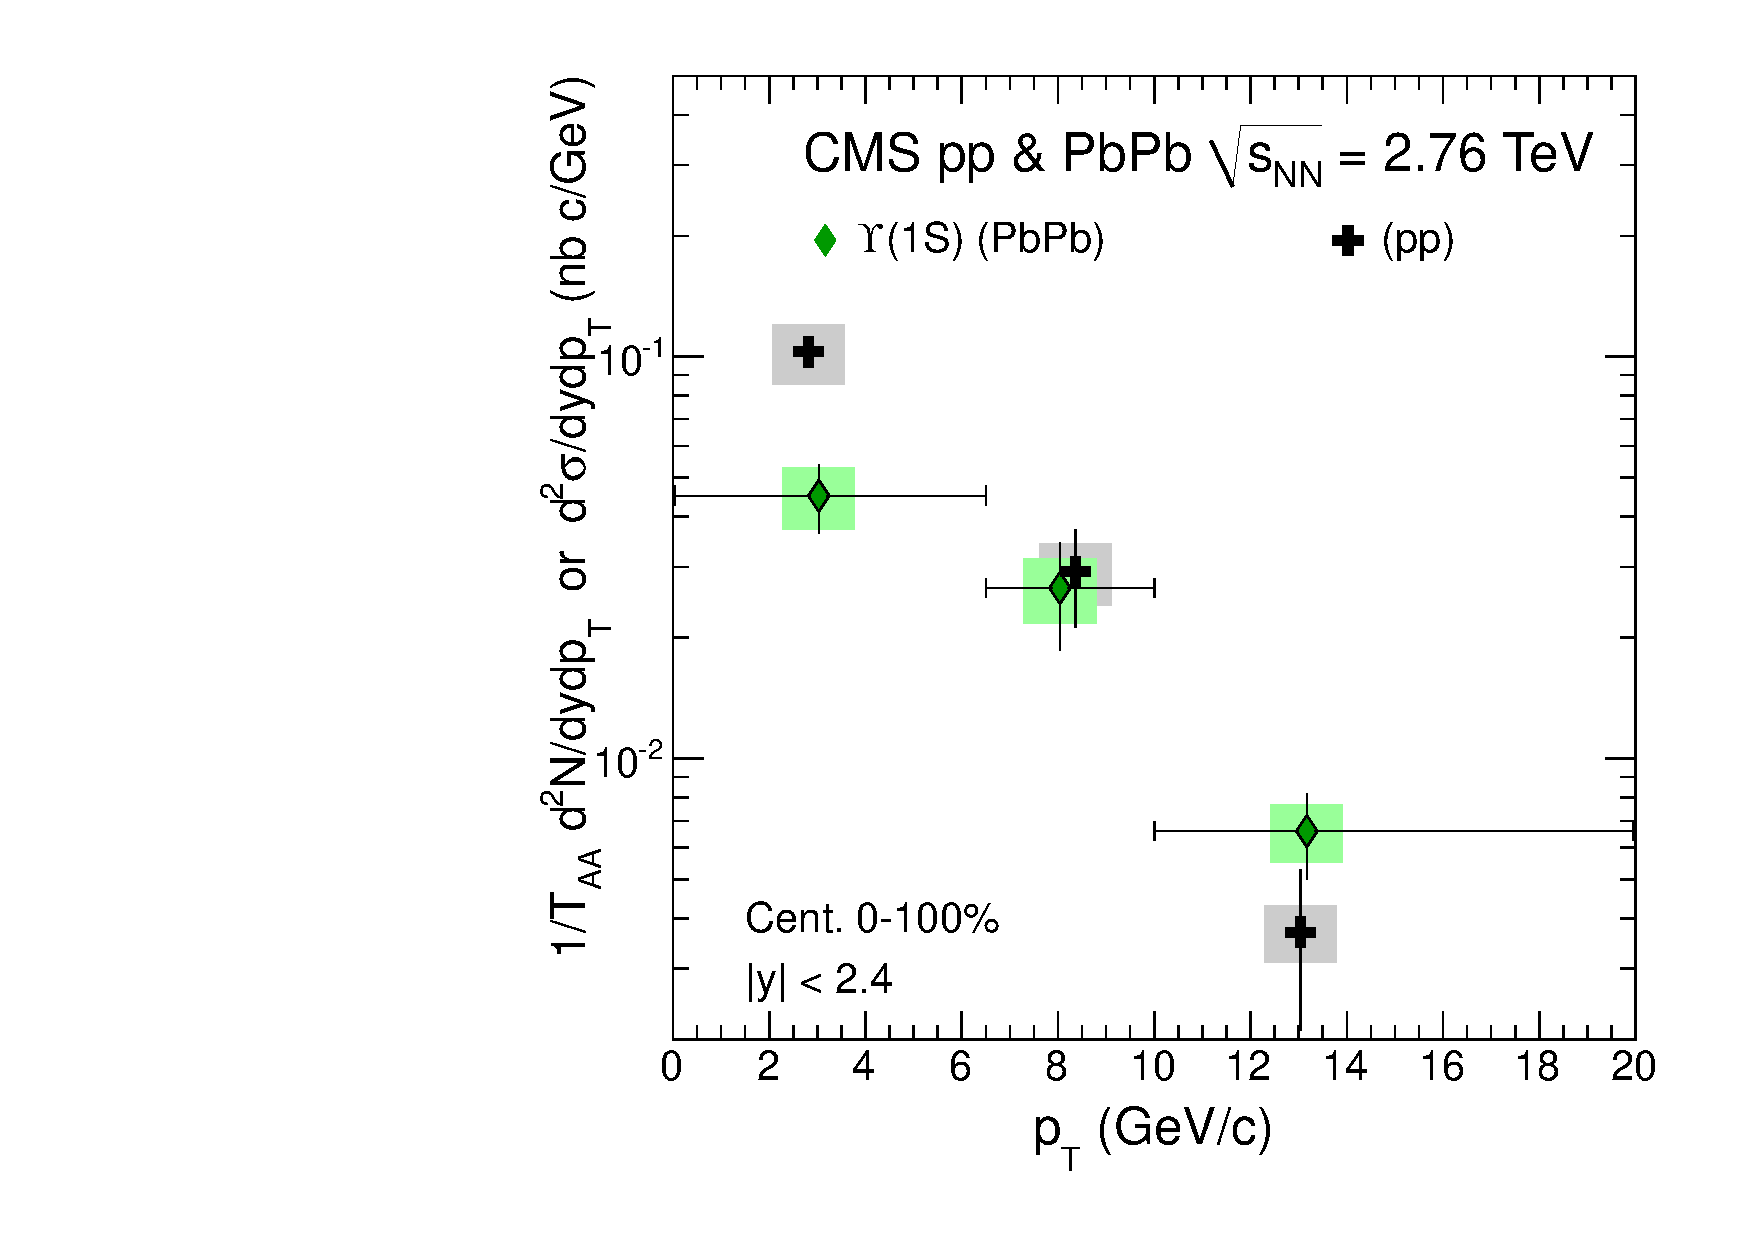
\includegraphics[width=0.45\textwidth]{chap_YInPbPbColl2010_figures/upsilon_pt}\hspace{1em}
    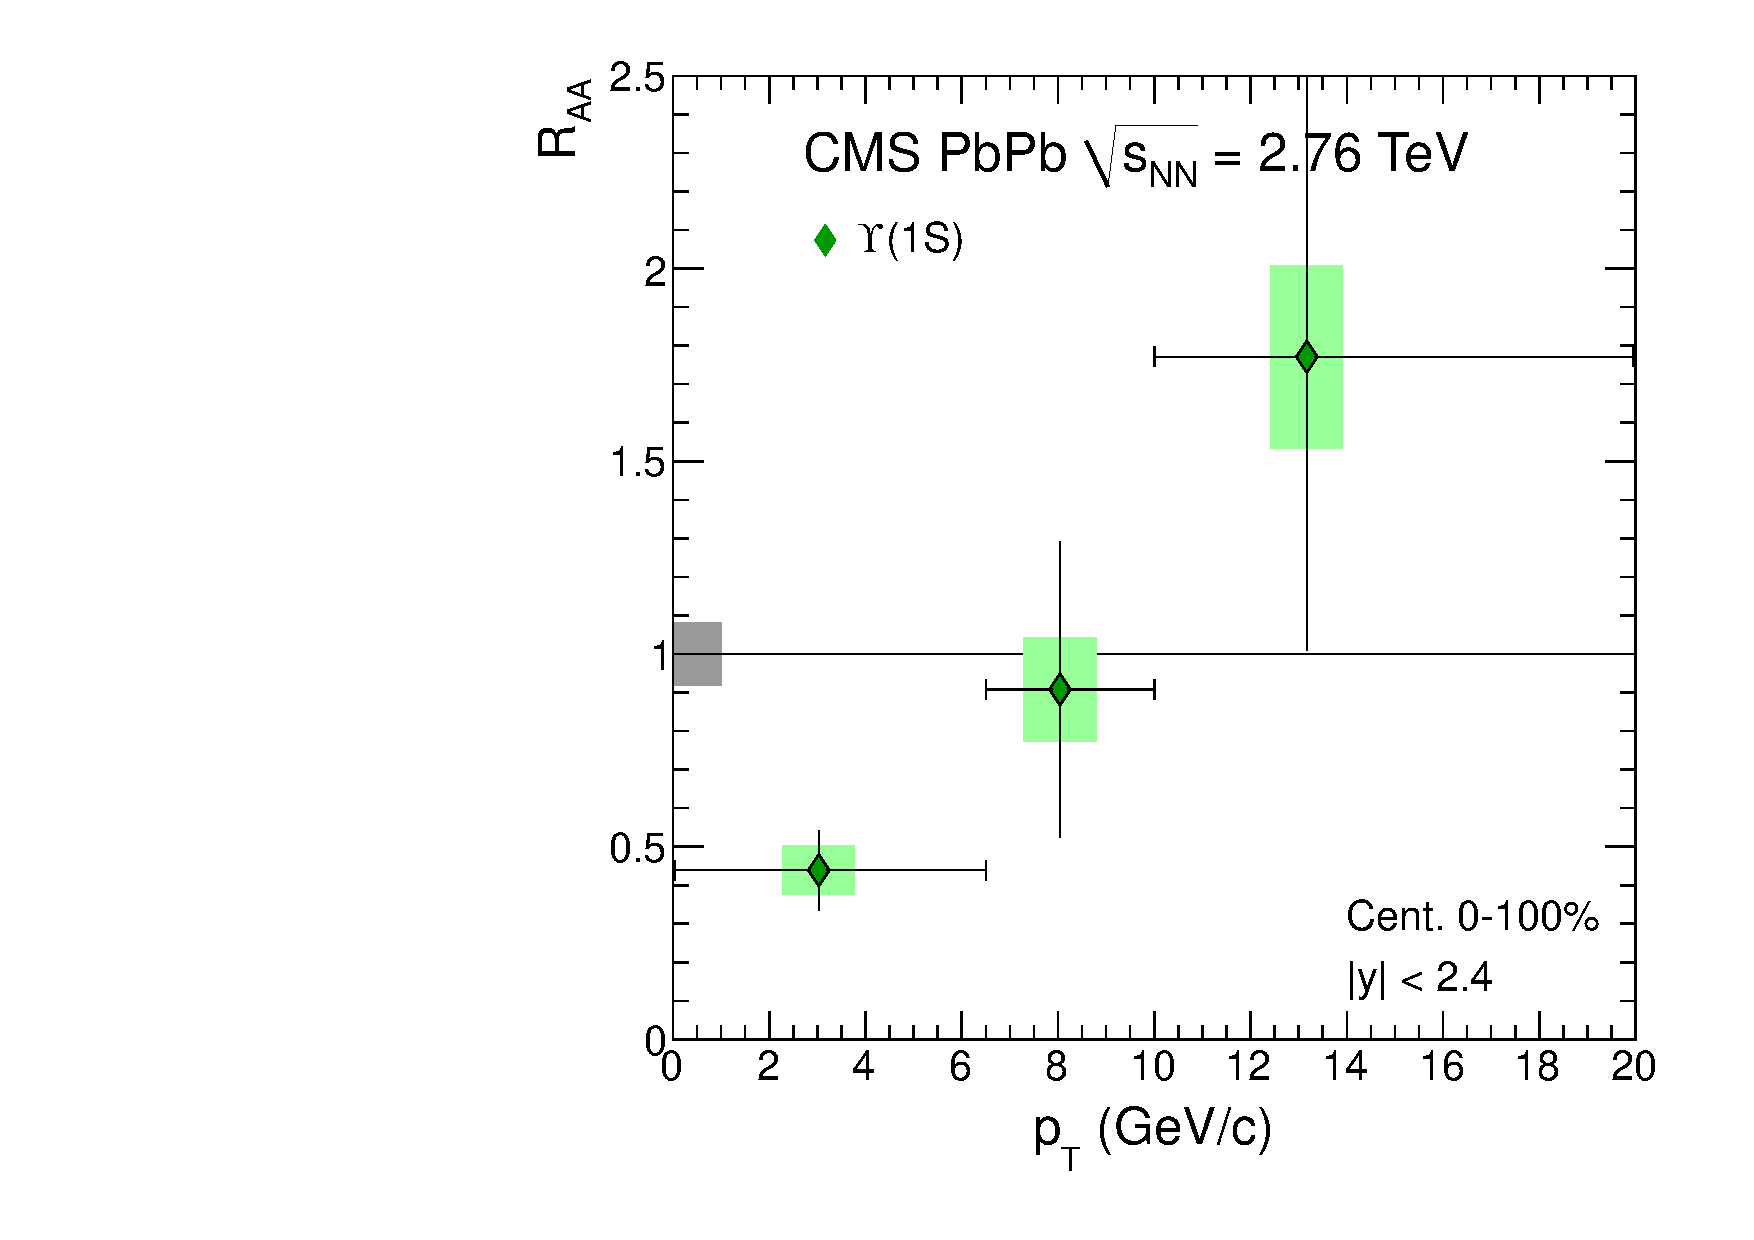
\includegraphics[width=0.45\textwidth]{chap_YInPbPbColl2010_figures/upsilon_RAA_pt}
    \caption{Left: \PgUa\ yield divided by \taa in \PbPb collisions
      (green diamonds) as a function of \pt. The result is compared to
      the cross section measured in \pp collisions (black crosses).
      The global scale uncertainties on the \PbPb data due to \taa
      (5.7\%) and the \pp integrated luminosity (6.0\%) are not
      shown. Right: nuclear modification factor \raa of \PgUa\ as a
      function of \pt. A global uncertainty of 8.3\%, from \taa and
      the integrated luminosity of the \pp data sample, is shown as a
      grey box at $\raa=1$. Points are plotted at their measured
      average \pt. Statistical (systematic) uncertainties are shown as
      bars (boxes). Horizontal bars indicate the bin width.}
    \label{fig:upsilon_pt}
  \end{center}
\end{figure}

\begin{figure}[htbp]
  \begin{center}
    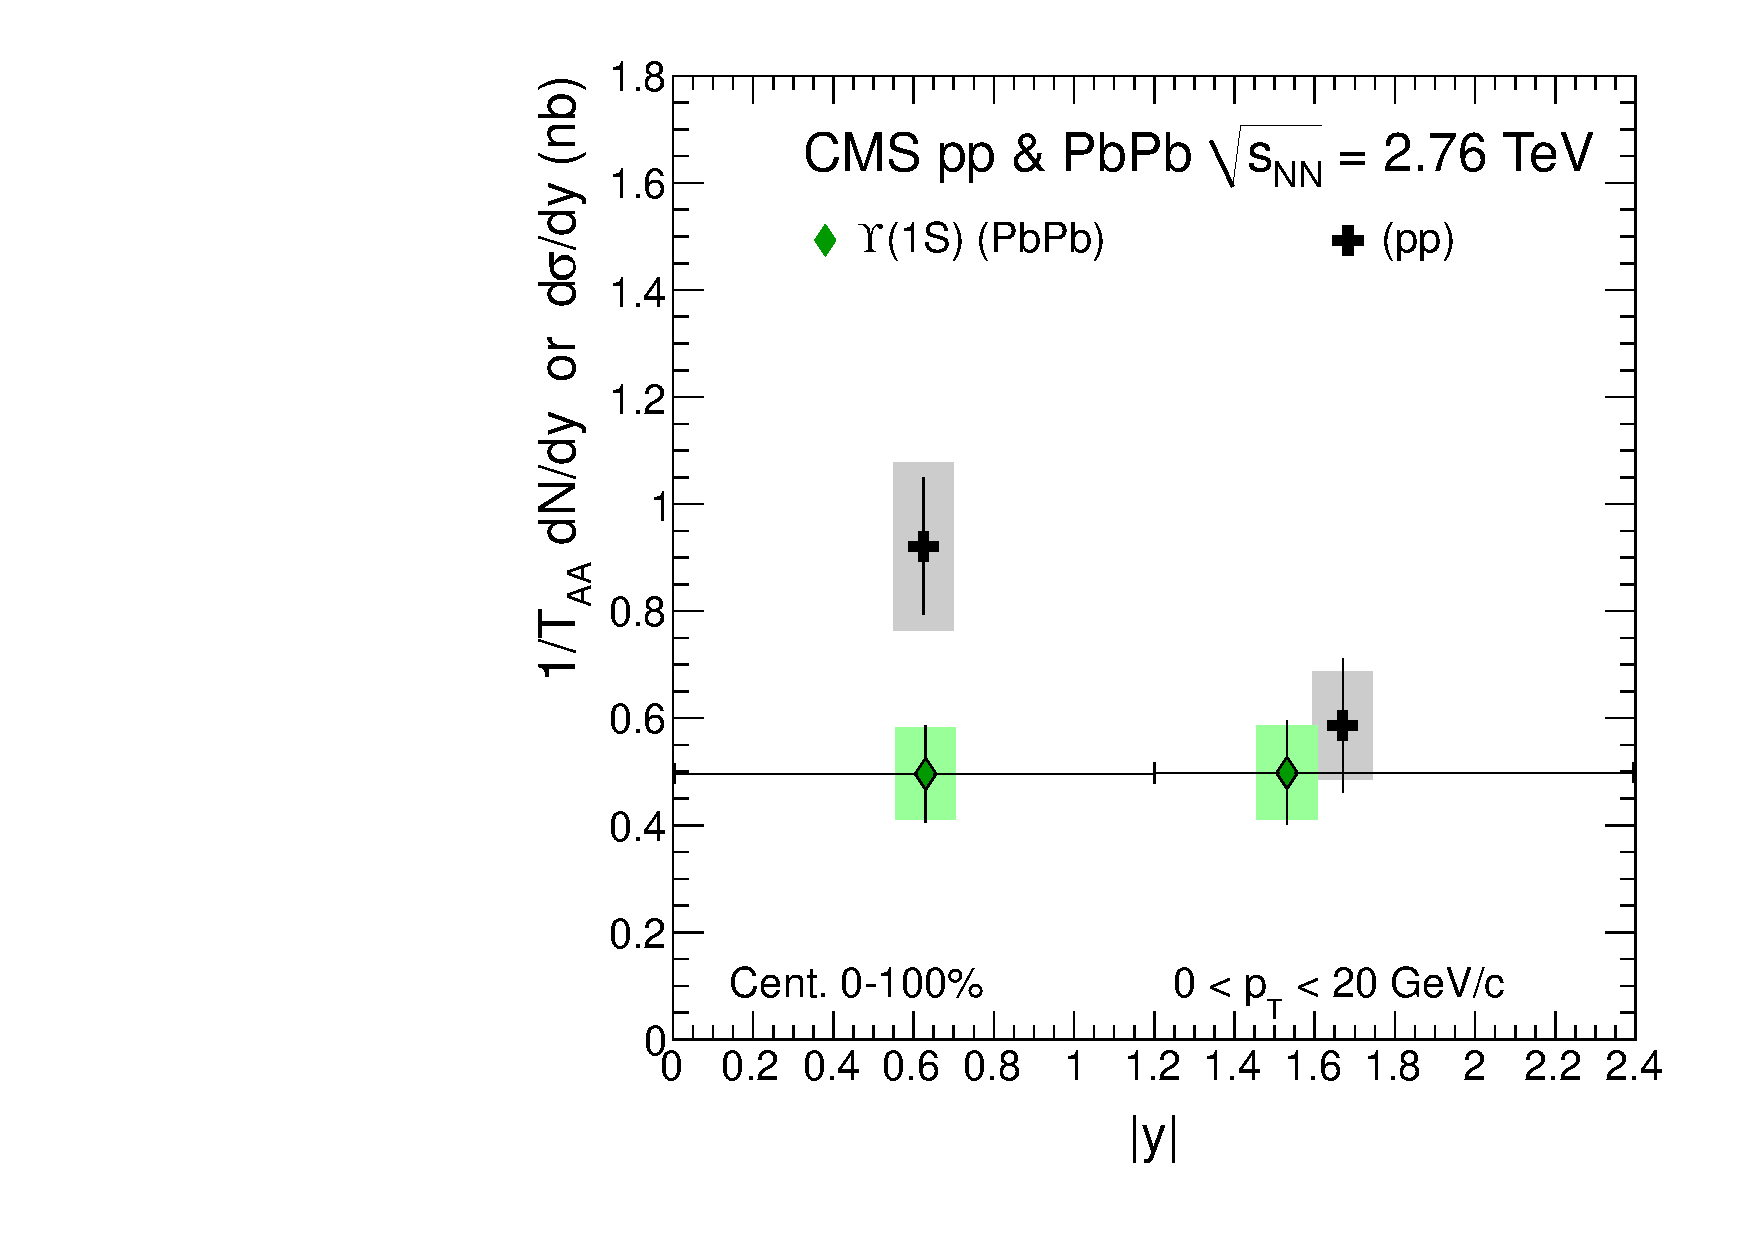
\includegraphics[width=0.45\textwidth]{chap_YInPbPbColl2010_figures/upsilon_eta}\hspace{1em}
    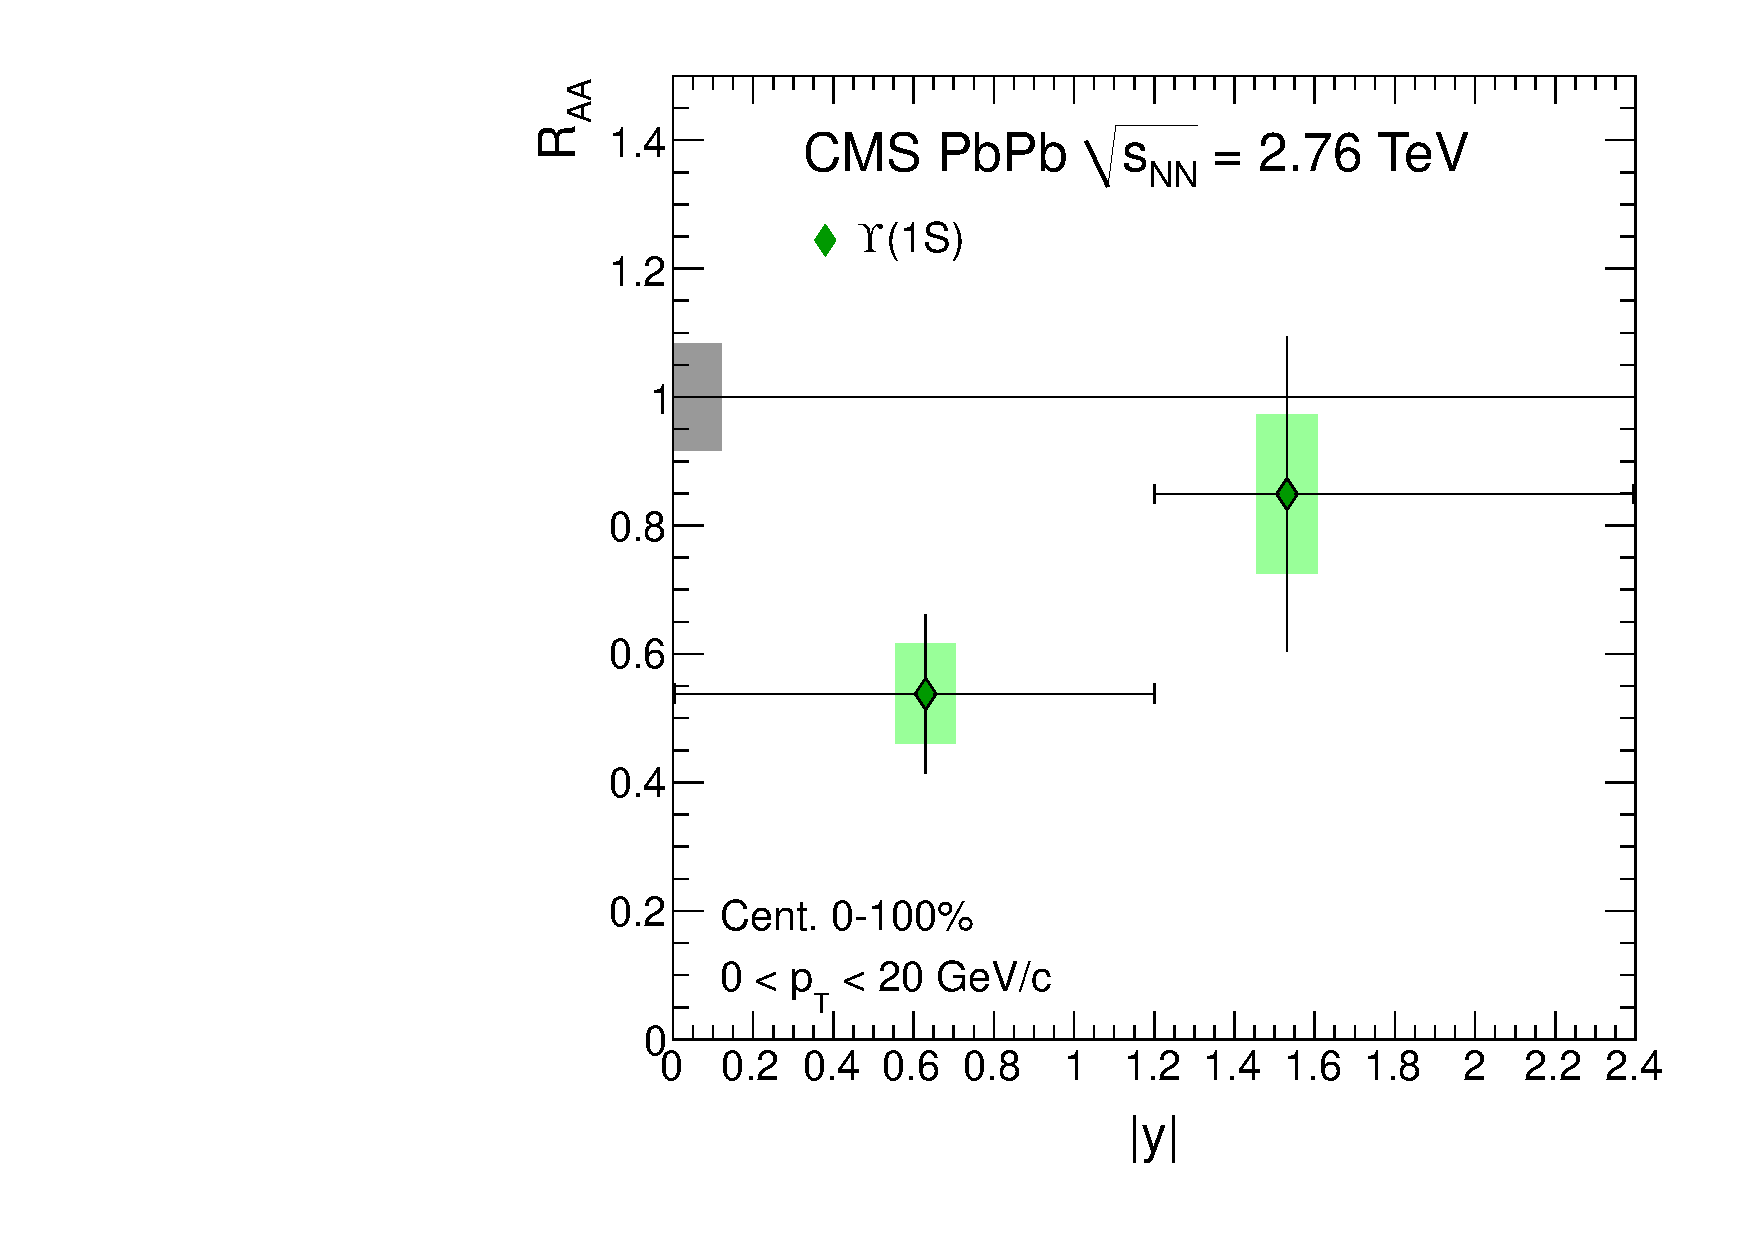
\includegraphics[width=0.45\textwidth]{chap_YInPbPbColl2010_figures/upsilon_RAA_eta}
    \caption{Left: \PgUa\ yield divided by \taa in \PbPb collisions
      (green diamonds) as a function of rapidity. The result is
      compared to the cross section measured in \pp collisions (black
      crosses). The global scale uncertainties on the \PbPb data due
      to \taa (5.7\%) and the \pp integrated luminosity (6.0\%) are
      not shown. Right: nuclear modification factor \raa of \PgUa\ as a
      function of rapidity. A global uncertainty of 8.3\%, from \taa
      and the integrated luminosity of the \pp data sample, is shown
      as a grey box at $\raa=1$. Points are plotted at their measured
      average $|y|$. Statistical (systematic) uncertainties are shown
      as bars (boxes). Horizontal bars indicate the bin width.}
    \label{fig:upsilon_eta}
  \end{center}
\end{figure}
\begin{figure}[htbp]
  \begin{center}
    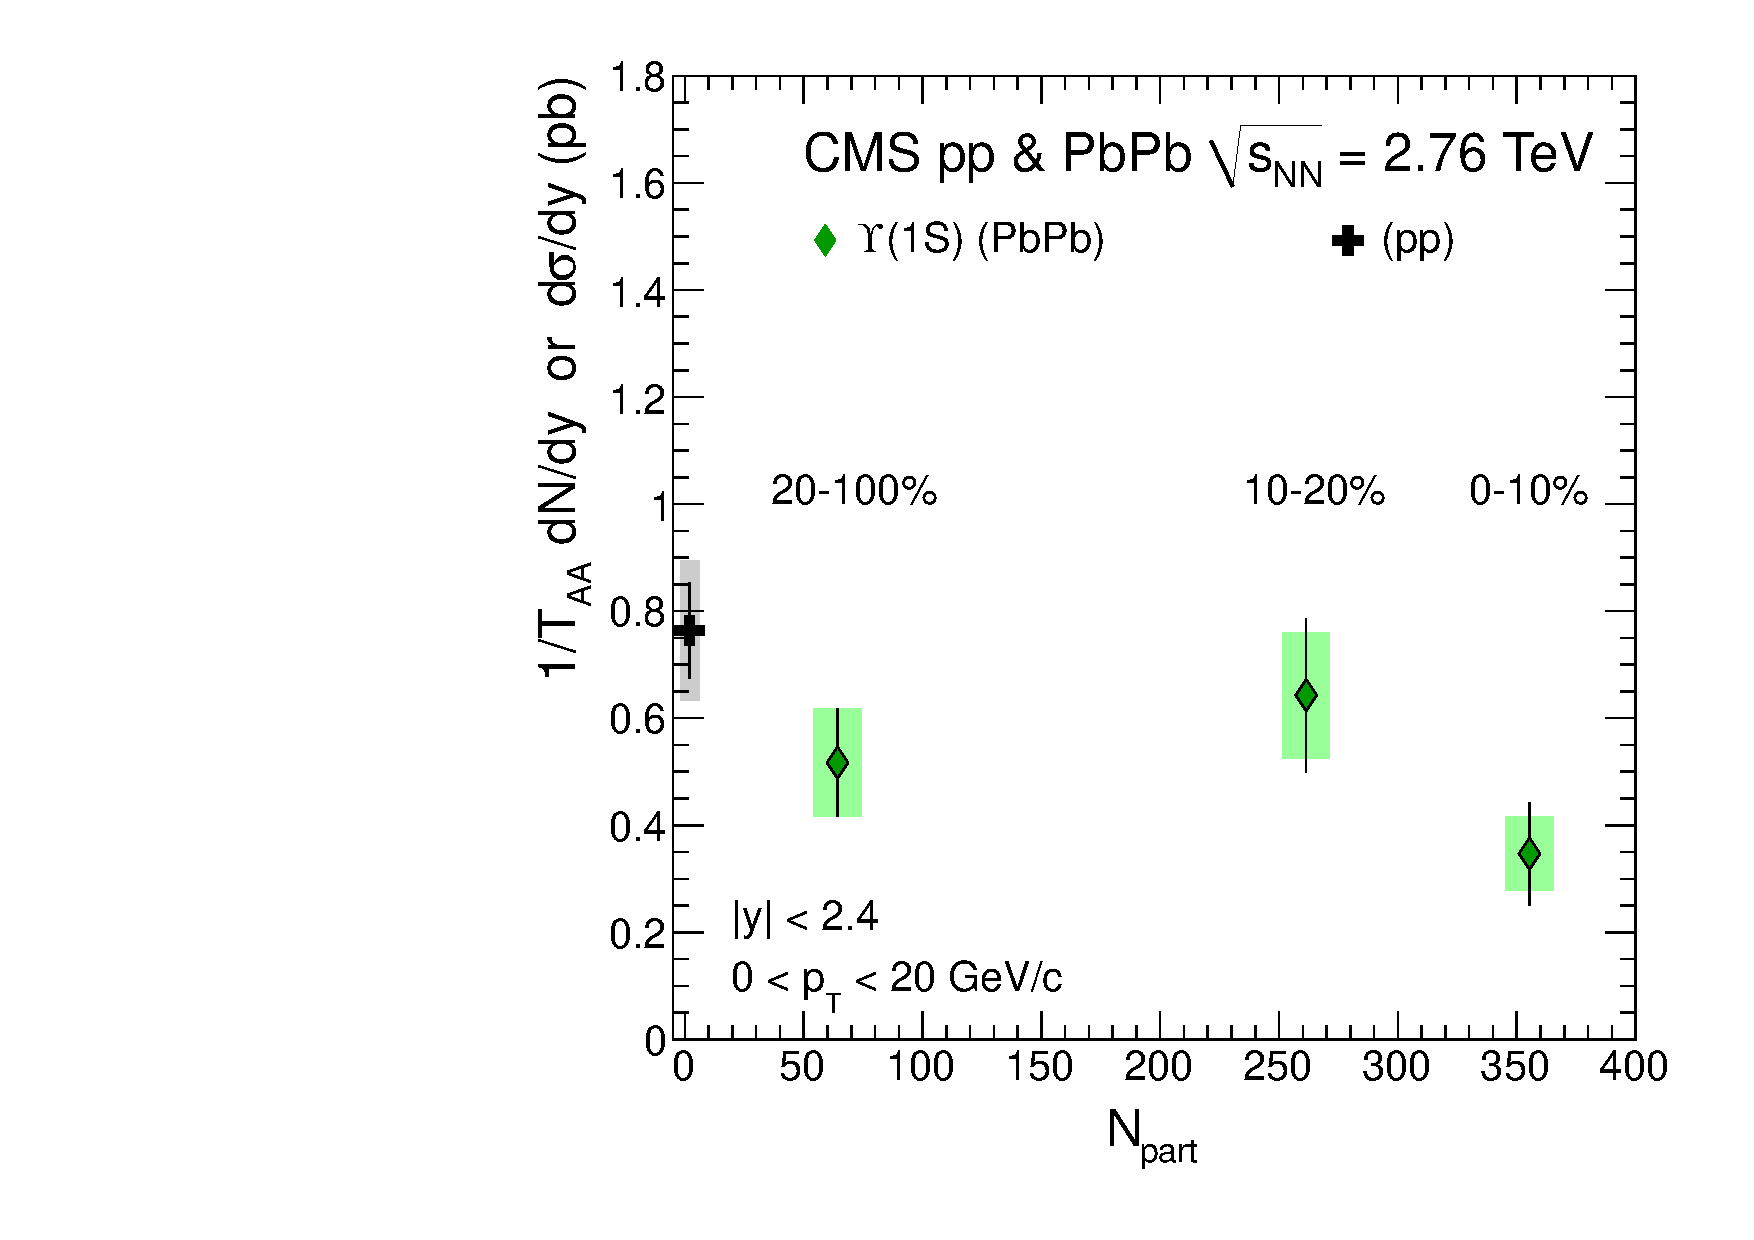
\includegraphics[width=0.45\textwidth]{chap_YInPbPbColl2010_figures/upsilon_cent}\hspace{1em}
    \includegraphics[width=0.45\textwidth]{chap_YInPbPbColl2010_figures/upsilon_RAA.pdf}
    \caption{Left: \PgUa\ yield divided by \taa (green diamonds) as a
      function of \npart compared to the \PgUa\ cross section measured
      in \pp (black cross). Right: nuclear modification factor \raa of
      \PgUa\ as a function of \npart. A global uncertainty of 6\%, from
      the integrated luminosity of the \pp data sample, is shown as a
      grey box at $\raa=1$. Statistical (systematic) uncertainties are
      shown as bars (boxes).}
    \label{fig:upsilon_cent}
  \end{center}
\end{figure}


\section{Indication of suppression of excited $\Upsilon$ states in PbPb collisions at $\sqrt{s_{\rm NN}} = 2.76$~TeV}
\label{sec:YDoubleRatio2010}
A comparison of the relative yields of $\Upsilon$ resonances in the $\mu^+\mu^-$ decay channel in PbPb and pp collisions at a centre-of-mass energy per nucleon pair 
of 2.76~TeV, is performed with data collected with the CMS detector at the LHC. Using muons of transverse momentum above 4~GeV/$c$ and pseudorapidity below 2.4, 
the double ratio of the $\Upsilon(2S)$ and $\Upsilon(3S)$ excited states to the $\Upsilon(1S)$ ground state in PbPb and pp collisions, 
$[\Upsilon(2S+3S)/\Upsilon(1S)]_{\rm PbPb} / [\Upsilon(2S+3S)/\Upsilon(1S)]_{\Pp\Pp}$, is found to be 0.31~$_{-0.15}^{+0.19}$~(stat.)~$\pm$~0.03~(syst.). 
The probability to obtain the measured value, or lower, if the true double ratio is unity, is calculated to be less than 1\%.
The measurement is performed with the data recorded by the Compact Muon Solenoid (CMS) experiment during the first PbPb LHC run, at the end of 2010, and during the 
pp run of March 2011, both at $\sqrt{s_{\rm NN}} = 2.76$~TeV. The integrated luminosity used in this analysis corresponds to 7.28~$\mu$b$^{-1}$ for PbPb and 
225~nb$^{-1}$ for pp collisions, the latter corresponding approximately to the equivalent nucleon-nucleon luminosity of the PbPb run. 
The excellent momentum resolution of the CMS detector results in well-resolved $\Upsilon$ peaks in the dimuon mass spectrum. 

A detailed description of the CMS detector can be found in~\ref{sec:YDoubleRatio2010}. Its central feature is a superconducting solenoid of 6~m internal diameter, 
providing a magnetic field of 3.8~T. Within the field volume are the silicon pixel and strip tracker, the crystal electromagnetic calorimeter, and the 
brass/scintillator hadron calorimeter. Muons are measured in gas-ionisation detectors embedded in the steel return yoke. In addition, 
CMS has extensive forward calorimetry, in particular two steel/quartz-fiber Cerenkov hadron forward (HF) calorimeters, which cover the pseudorapidity 
range $2.9 < |\eta| < 5.2$.

In this analysis, $\Upsilon$ mesons are identified through their dimuon decay. The silicon pixel and strip tracker measures charged-particle 
trajectories in the  range $|\eta| < 2.5$. The tracker consists of 66M pixel and 10M strip detector channels, providing a vertex resolution of 
$\sim$\,15~$\mu$m in the transverse plane. Muons are detected in the $|\eta| < 2.4$ range, with detection planes based on three technologies: 
drift tubes, cathode strip chambers, and resistive plate chambers. Due to the strong magnetic field and the fine granularity of the silicon tracker, 
the muon transverse momentum measurement ($p_{\rm T}$) based on information from the silicon tracker alone has a resolution between 
1 and 2$\%$ for a typical muon in this analysis.

In both the PbPb and pp runs, the events are selected by the CMS two-level trigger. At the first, hardware level, two independent muon candidates are 
required in the muon detectors. No selection is made on momentum or pseudorapidity, but in the pp case more stringent quality requirements are imposed 
for each muon in order to reduce the higher trigger rate. In both cases, the software-based higher-level trigger accepts the lower-level decision without 
applying further criteria. From reconstructed $J/\psi \rightarrow \mu\mu$ decays, the single-muon trigger efficiencies are measured and found to be consistent 
between the PbPb, $(96.1 \pm 1.0)\%$, and the pp, $(95.5 \pm 0.6)\%$, data sets, for muons with $p_{\rm T} >$~4~GeV/$c$.

In the PbPb data, events are preselected offline if they contain a reconstructed primary vertex made of at least two tracks, and a coincidence in both 
HF calorimeters of energy deposits in at least three towers of 3~GeV each. These criteria reduce contributions from single-beam interactions 
(e.g. beam-gas and beam-halo collisions with the beam pipe), ultra-peripheral electromagnetic collisions, and cosmic-ray muons. A small fraction of 
the most peripheral PbPb collisions is not selected by these requirements, which accept $(97 \pm 3)$\% of the hadronic inelastic 
cross section. For the pp run, a similar event filter is applied, relaxing the HF coincidence to one tower in each HF, with at least 3~GeV deposited. 
This filter removes only 1$\%$ of the pp events satisfying the dimuon trigger.

The muon offline reconstruction is seeded with $\simeq 99\%$ efficiency by tracks in the muon detectors, called standalone muons. 
These tracks are then matched to tracks reconstructed in the silicon tracker by means of an algorithm optimised for the 
heavy-ion environment~\cite{Roland:2006kz,D'Enterria:2007xr}. For muons from $\Upsilon$ decays the tracking efficiency is $\simeq$~85\%. 
This efficiency is lower than in pp, as in PbPb the track reconstruction is seeded by a greater number of pixel hits to reduce the large number 
of random combinations arising from the high multiplicity of each event. Combined fits of the muon and tracker tracks are used to obtain the 
results presented in this section. The heavy-ion dedicated reconstruction algorithm is applied to the pp data in order to avoid potential biases, 
arising from different tracking efficiencies of the two reconstruction algorithms, when comparing the two data sets.

Identical very loose selection criteria are applied to the muons in the pp and PbPb data. The transverse (longitudinal) distance from the event 
vertex is required to be less than 3 (15) cm. Tracks are only kept if they have 11 or more hits in the silicon tracker and the $\chi^2$ per degree 
of freedom of the combined (tracker) track fit is lower than 20 (4). The two muon trajectories are fit with a common vertex constraint, 
and events are retained if the fit $\chi^2$ probability is larger than 1$\%$. This removes background arising primarily from displaced heavy 
quark semileptonic decays. As determined from Monte Carlo simulation of the $\Upsilon(1S)$ signal, these selection criteria are found to 
reduce the efficiency by 3.9$\%$, consistent with the signal loss observed in both pp and PbPb data. The available event sample limits to 
20~GeV/$c$ the dimuon transverse momentum range probed in this study.

In order to further reduce the background in the $\Upsilon$ mass region, only muons with a transverse momentum ($p_{\rm T}^\mu$) higher than 
4~GeV/$c$ are considered, resulting in a $\Upsilon$ acceptance of approximately 25$\%$  for the $|y^\Upsilon|<2.4$ rapidity range. This 
requirement improves the significance of the $\Upsilon(1S)$ signal in PbPb data and is applied to both data sets. The acceptance of 
a $\Upsilon$ state depends on its mass, since the excited states give rise to higher-momenta muons. In consequence, requiring higher 
$p_{\rm T}^\mu$ increases the acceptance for the excited states relative to the ground state. 
In the corresponding analysis performed with the higher-statistics (3.1~pb$^{-1}$) 7~TeV data~\cite{Khachatryan:2010zg}, looser criteria were applied 
($p_{\rm T}^\mu >$~3.5 GeV/$c$ and $|\eta^\mu| < 1.6$, or $p_{\rm T}^\mu >$2.5 GeV/$c$ and $1.6 < |\eta^\mu| < 2.4$), where $\eta^\mu$ is the muon pseudorapidity. 
The stricter ($p_{\rm T}^\mu >$~4~GeV/$c$) requirements used here  enhance the  $\Upsilon(2S+3S)/\Upsilon(1S)$ yield ratio by $\simeq 60$\% in the \Pp\Pp\ data 
at 2.76~TeV. It was checked that, applying the same reconstruction algorithm and the same $p_{\rm T}^\mu$ requirements, the $\Upsilon(2S+3S)/\Upsilon(1S)$ yield 
ratio is consistent between the 2.76 and 7~TeV pp data sets.
The dimuon invariant mass spectra with the selection criteria applied are shown in Fig.~\ref{fig:massY2010} for the pp and PbPb data sets. Within the 7--14~GeV/$c^2$ 
mass range, there are 561 (628) opposite-sign muon pairs in the pp (PbPb) data set. The three Y peaks are clearly observed in the pp case, but the 
$\Upsilon(2S)$ and $\Upsilon(3S)$ are barely visible over the residual background in PbPb collisions.

\begin{figure}[hbtp]
  \begin{center}
    \includegraphics[width=0.95\linewidth]{chap_YInPbPbColl2010_figures/Mass_pp.pdf} 
    \includegraphics[width=0.95\linewidth]{chap_YInPbPbColl2010_figures/Mass_PbPb_nofit.pdf} 
    \caption{Dimuon invariant-mass distributions from the \Pp\Pp\ (a) and PbPb (b) data at $\sqrt{s_{\rm NN}} = 2.76$~TeV. 
      The same reconstruction algorithm and analysis criteria are applied to both data sets, including a transverse momentum requirement on 
      single muons of $p_{\rm T}^\mu >$~4~GeV/$c$. The solid lines show the result of the fit described in the text.}
    \label{fig:massY2010}
  \end{center}
    \vspace{-2ex}
\end{figure}
An extended unbinned maximum likelihood fit to the two invariant mass distributions of Fig.~\ref{fig:mass} is performed to extract the yields, following the 
method described in~\cite{Khachatryan:2010zg}. The measured mass lineshape of each $\Upsilon$ state is parameterised by a ``Crystal Ball'' (CB) function, i.e. 
a Gaussian resolution function with the low-side tail replaced by a power law describing final state radiation (FSR). Since the three $\Upsilon$ resonances partially 
overlap in the measured dimuon mass, they are fit simultaneously. Therefore, the probability distribution function (PDF) describing the signal consists of three CB 
functions. In addition to the three $\Upsilon(nS)$ yields, the $\Upsilon(1S)$ mass is the only parameter left free, to accommodate a possible bias in the momentum 
scale calibration. The mass differences between the states are fixed to their world average values~\cite{Nakamura:2010zzi} and the mass resolution is forced to scale 
with the resonance mass. The $\Upsilon(1S)$ resolution is fixed to the value estimated in the simulation, 92~MeV/$c^2$, which is compatible with the resolution obtained 
from both the PbPb and pp data. The low-side tail parameters are also fixed to the values obtained via simulation. Finally, a second-order polynomial is chosen to 
describe the background in the 7--14~GeV/$c^2$ mass-fit range.
The quality of the unbinned fit is checked \emph{a posteriori} by comparing the obtained lineshapes to the binned data of Fig.~\ref{fig:massY2010}. 
The $\chi^2$ probabilities are 74$\%$ and 77$\%$, respectively for pp and PbPb.

The ratios of the observed yields of the $\Upsilon(2S)$ and $\Upsilon(3S)$ excited states to the $\Upsilon(1S)$ ground state in the pp and PbPb data are:
\begin{eqnarray}
  \Upsilon(2S+3S)/\Upsilon(1S)|_{\Pp\Pp} & = & 0.78 _{-0.14}^{+0.16} \pm 0.02,\\
  \Upsilon(2S+3S)/\Upsilon(1S)|_{\rm PbPb} & = & 0.24 _{-0.12}^{+0.13} \pm 0.02,
\end{eqnarray}
where the first uncertainty is statistical and the second is systematic.

The systematic uncertainties are computed by varying the lineshape in the following ways: 
\begin{enumerate}
\item the CB-tail parameters are varied randomly according to their covariance matrix and within conservative values covering imperfect 
knowledge of the amount of detector material and FSR in the underlying process; 

\item the resolution is varied by $\pm 5$~MeV/$c^2$, which is a conservative variation given the current understanding of the detector performance 
and reasonable changes that can be anticipated in the $\Upsilon$-resonance kinematics between pp and PbPb data; 

\item the background shape is changed from quadratic to linear while the mass range of the fit is varied from 6--15 to 8--12~GeV/$c^2$; 
\end{enumerate}
the observed root-mean-square of the results is taken as the systematic uncertainty. The quadrature sum of these three systematic uncertainties 
gives a relative uncertainty on the ratio of 10$\%$ (3$\%$) on the PbPb (pp) data.

The ratio of the $\Upsilon(2S+3S)/\Upsilon(1S)$ ratios in PbPb and pp benefits from an almost complete cancellation of possible acceptance 
and/or efficiency differences among the reconstructed resonances. A simultaneous fit to the pp and PbPb mass spectra gives the double ratio
\begin{equation}
  \frac{\Upsilon(2S+3S)/\Upsilon(1S)|_{\rm PbPb}}{\Upsilon(2S+3S)/\Upsilon(1S)|_{\Pp\Pp}}
 = 0.31 _{-0.15}^{+0.19} \; ({\rm stat.}) \pm 0.03 \; ({\rm syst.}),
\label{eq:double}
\end{equation}
where the systematic uncertainty (9$\%$) arises from varying the lineshape as described above in the simultaneous fit, 
thus taking into account partial cancellations of systematic effects.

To evaluate possible imperfect cancellations of acceptance and efficiency effects in the double ratio, a full GEANT4~\cite{Agostinelli:2002hh} detector 
simulation is performed. The effect of the higher PbPb underlying event activity is considered by embedding, at the level of detector signals, $\Upsilon(1S)$ 
and $\Upsilon(2S)$ decays simulated by PYTHIA 6.424~\cite{Sjostrand:2006za} in PbPb events simulated with \textsc{hydjet}~\cite{Lokhtin:2005px}. 
Track characteristics, such as the number of hits and the $\chi^2$ of the track fit, have similar distributions in data and simulation. As mentioned above, the 
trigger efficiency is evaluated with data, by using single-muon-triggered data events, and reconstructing J/$\psi$ signal with and without the dimuon trigger requirement. 
The same exercise is carried out with the simulation and it agrees with the efficiency measured in data at the 2$\%$ level. The track efficiency in the silicon detector 
is measured with standalone muons, applying all selection criteria. The efficiencies in data and simulation agree within the 4$\%$ statistical uncertainty of the 
efficiency determined from data.
The difference in reconstruction and selection efficiencies between the $\Upsilon$ states is less than 5$\%$ and the variation with charged particle multiplicity is less 
than 10$\%$ from pp to central PbPb collisions, producing a maximum change of 0.5$\%$ on the double ratio. The good agreement between single-muon trigger efficiencies 
extracted from data for the pp and PbPb trigger requirements, applied to the $\Upsilon(1S)$ and $\Upsilon(2S)$ trigger efficiencies derived from simulation, leads to a 
negligible effect on the double ratio. The single-muon trigger efficiencies extracted from data agree within 1.5$\%$ for the pp and PbPb trigger requirements, and the 
$\Upsilon(1S)$ and $\Upsilon(2S)$ trigger efficiencies agree within 3$\%$, according to simulation: the potential trigger bias on the double ratio is negligible. 
The magnitudes of the statistical and systematic uncertainties on the double ratio, respectively 55$\%$ and 9$\%$, are significantly larger than the systematic 
uncertainties associated with possible imperfect cancellation of acceptance and efficiency effects. Therefore no additional uncertainty from these sources is applied.
Finally, using an ensemble of one million pseudo-experiments, generated with the signal lineshape obtained from the pp data (Fig.~\ref{fig:massY2010}a), the background 
lineshapes from both data sets, and a double ratio (Eq.~\ref{eq:double}) equal to unity within uncertainties, the probability of finding the measured value of 0.31 or 
below is estimated to be 0.9$\%$. In other words, in the absence of a suppression due to physics mechanisms, the probability of a downward departure of the ratio from 
unity of this significance or greater is 0.9$\%$, i.e. that corresponding to 2.4 sigma in a one-tailed integral of a Gaussian distribution.
Studies in section \ref{sec:results} show that the $\Upsilon(1S)$ itself is suppressed by about 40$\%$ in minimum bias PbPb collisions at 
$\sqrt{s_{\rm NN}} = 2.76$~TeV. Since a large fraction of the $\Upsilon(1S)$ yield arises from decays of heavier bottomonium states~\cite{Affolder:1999wm}, 
this $\Upsilon(1S)$ suppression could be indirectly caused by the suppression of the excited states.

Production yields of quarkonium states can also be modified, from pp to PbPb collisions, in the absence of QGP formation, by cold nuclear matter effects~\cite{Vogt:2010aa}. 
However, such effects should have a small impact on the $\Upsilon$ double ratio reported here. The nuclear modifications of the parton distribution functions (shadowing) 
should have an equivalent effect on the three $\Upsilon$ states, because their production involves very similar partons, cancelling in the ratio, at least to first order. 
The same should happen to any other initial-state nuclear effect. In principle, the larger and more loosely bound excited quarkonium states are more likely to be broken 
up by final-state interactions while traversing the nuclear matter, something extensively studied in the context of charmonium suppression at lower energies
~\cite{Lourenco:2008sk}. 
This ``nuclear absorption'' becomes weaker with increasing energy, and should be negligible at the LHC. At RHIC energies, the STAR experiment~\cite{Reed:2011zz} has reported 
a $\Upsilon(1S+2S+3S)$ yield in dAu collisions of $0.78 \pm 0.28 \pm 0.20$ times the yield expected by scaling pp collisions, compatible with the absence of absorption. 
Furthermore, the double ratio presented here would only be sensitive to a \emph{difference} between the nuclear dependencies of the three states and already at much lower energies 
the Fermilab E772 experiment observed~\cite{Alde:1991sw}, in proton-nucleus collisions, no such difference, within uncertainties, between the $\Upsilon(1S)$ and 
the sum $\Upsilon(2S+3S)$.





\section{Discussion}
\label{sec:discussion}
The \PgUa\ yield divided by \taa as a function of \pt, rapidity, and
centrality has been measured in \PbPb collisions.  No strong
centrality dependence is observed within the uncertainties. The
nuclear modification factor integrated over centrality is $\raa =
0.63\pm0.11\,(\text{stat.})\pm0.09\,(\text{syst.})$. This suppression
is observed predominantly at low \pt. Using \ppbar collisions at
\sqrts = 1.8\TeV, CDF measured the fraction of directly produced \PgUa\
as $(50.9\pm8.2\,(\text{stat.})\pm9.0\,(\text{syst.}))\%$ for \PgUa\
with $\pt>8\GeVc$~\cite{Affolder:1999wm}. Therefore, the \PgUa\
suppression presented in this paper could be indirectly caused by the
suppression of excited \PgU\ states.
Comparison of the relative yields of $\Upsilon$ resonances has been performed in PbPb and pp collisions at the same 
centre-of-mass energy per nucleon pair of 2.76 TeV. The double ratio of the $\Upsilon(2S)$ and $\Upsilon(3S)$ excited states to the $\Upsilon(1S)$ 
ground state in PbPb and pp collisions, $[\Upsilon(2S+3S)/\Upsilon(1S)]_{\rm PbPb}/[\Upsilon(2S+3S)/\Upsilon(1S)]_{\Pp\Pp}$, is found to be 
0.31~$_{-0.15}^{+0.19}$~(stat.)~$\pm$~0.03~(syst.), for muons of $p_{\rm T}>4$~GeV/$c$ and $|\eta|<2.4$. 
The probability to obtain the measured value, or lower, if the true double ratio is unity, has been calculated to be less than 1\%. 

  
  \chapter{Detail study of $\Upsilon$ suppression in Pb+Pb collisions using 150 $\mu$b$^{-1}$ data with CMS detector at LHC.} 
\label{chap:UpsilonProductionPbPb2011}

\section{Introduction}
\label{sec:introduction}
I modify.
The LHC allows for the first detailed studies of the bottomonium family of states in ultra-relativistic 
heavy-ion collisions. Given the momentum resolution attained, and the capability of the trigger system,  
CMS is well positioned to lead these studies. The measurement of bottomonium production and suppression is 
presented, based on the dataset collected by the CMS experiment during the 2011 PbPb collision run at  $\sqrtsnn = 2.76\TeV$. 

If a deconfined medium is formed in high-energy heavy-ion collisions, one of its most striking expected characteristics is the 
suppression of quarkonium states~\cite{Matsui:1986dk}. 
This takes place as the force between the constituents of the quarkonium state, a heavy quark and its antiquark, is weakened by 
the color screening produced by the surrounding light quarks and gluons.
The suppression is predicted to occur above a critical temperature of the medium, and sequentially, in the
order of the \QQbar binding energy. 
Since the \PgUa is the most tightly bound state among all quarkonia, it is expected to be the one
with the highest dissociation temperature. % in the QGP.
Such a suppression pattern is expected to further depend on complications arising from additional phenomena sometimes referred to as
$hot$ and $cold$ nuclear matter effects~\cite{Brambilla:2010cs,Vogt:2010aa}. 
%
The study of charmonium (\Jpsi, $\psi'$, $\chi_c$) and bottomonium ($\PgUa, \PgUb, \PgUc$, $\chi_b$) production at the unprecedented medium 
created at the LHC is accordingly much awaited.  
In this chapter, the measurements of the production and suppression of the $\PgUa$,  $\PgUb$, and  $\PgUc$ states are performed. 
The production of $\PgU$(nS) states is studied by comparing their production rates in PbPb and pp collision data, taken at the same collision 
energy of $\sqrt{s_{NN}}=2.76\,\TeV$.
In particular, the yield of the higher-mass states is measured relative to the ground state. In this way, we explore the double ratios  
--  $\PgU(2S,3S)~vs~\PgUa$ and \PbPb~$vs~\pp$ --which allows a self-calibrating measurement.  
%
Several effects associated to selection, acceptance, and reconstruction mostly cancel, and only remaining factors need to be accounted for,  
as corrections to the fitted ratio of raw signal yields.  
Based on the dataset collected during the first LHC PbPb run, at $\sqrtsnn = 2.76\TeV$, in 2010, and in the special $\Pp\Pp$ run at the 
same energy in early 2011, CMS has published first results on upsilon production and suppression in PbPb collisions. 
%
These included the first evidence for suppression of the excited $\PgU$ states relative to the ground state, at the $2.4\,\sigma$ level as 
discussed in chapter\ref{chap:UpsilonProductionPbPb2010}.%~\cite{prl,QM2011}. 
Suppression of the $\PgUa$ state, relative to $\Pp\Pp$ collisions at the same energy, has also been measured~\cite{prl,QM2011}. 
These two measurements were found to be consistent with suppression of only the excited states, which result in reduced feeddown 
from excited to ground states. These main results may be summarized as follows:
%
\begin{linenomath}
\begin{eqnarray}
  \PgU(2S+3S)/\PgUa|_{\PbPb} & = & 0.24 _{-0.12}^{+0.13} \pm 0.02\,, \nonumber \\
  \PgU(2S+3S)/\PgUa|_{\pp} & = & 0.78 _{-0.14}^{+0.16} \pm 0.02\,,  \nonumber \\
(\chi \equiv)
  \frac{\PgU(2S+3S)/\PgUa|_{\PbPb}}{\PgU(2S+3S)/\PgUa|_{\pp}}
 & = & 0.31 _{-0.15}^{+0.19} \pm 0.03 \,,  \nonumber \\
(\raa \equiv)
 \frac{\PgUa|_{\PbPb;\, 0-20\%}}{\PgUa|_{\pp}}
& = & 0.681 \pm 0.143 \pm 0.119 \,.  \nonumber
%\label{eq:intro-rat}
\end{eqnarray}
\end{linenomath}
In the 2011 PbPb run, CMS collected a dataset approximately 20 times larger than that gathered in 2010. 
These data will be scrutinized, in order to extract further novel and precision results, during the 
few years ensuing datataking.
In what follows, the corresponding analysis of upsilon suppression is detailed.


\section{Data Selection}
\label{sec:dataselection}
The data analysis starts with the Onia2MuMu skim which contains all pairs of global muons with an invariant mass larger than 2 \GeVc. 
All charge combinations are considered and all possible combinations within an event are kept.
The package that was used for the skimming can be found in CVS under CMSSW/HeavyFlavorAnalysis/Onia2MuMu.
Starting from this skim a TTree is filled with single muons and muon pairs that pass quality
criteria to reject the background of fake muons while keeping the efficiency of selecting real muons high.

In order to select good quality muons, different variables were studied. This section describes how the cuts are defined and what is 
the final set of quality criteria that used in the analysis. These might not be very important for a ratio analysis but it is also a 
preparation for a more detailed analysis of the nuclear modification factor.

Muon candidates are selected if reconstructed as \emph{global muons}. Muon arbitration requirements are applied, 
specifically muons must be both global and tracker muons (accessed via the standard methods {\tt{isGlobal()}} and {\tt{isTracker()}}). 
Muon candidates are accepted if belonging to the kinematic region given by 
%
\begin{linenomath}
\begin{equation}
|\eta^\mu|<2.4 \quad \text{and} \quad \pt^\mu>4.0 \GeVc \,.
\label{eqn:muon_acc}
\end{equation}
\end{linenomath}
%
where the single muon \pt cut was determined with the optimization procedure described below.
This region is within acceptance for muon reconstruction. The optimal muon \pt threshold for the analysis is 
investigated in Sec.~\ref{sec:shoulder}.

\subsection{Optimization procedure}
The leading figure of merit employed in the optimization study is the $\PgUa$ {peak significance}, ${\cal{S}}$, defined as
%
\begin{linenomath}
\begin{equation}
{\cal{S}} \equiv \frac{N_\text{signal}}{\sqrt{N_\text{signal}+N_\text{background}}} \,,
\label{eqn:peak_signif}
\end{equation}
\end{linenomath}
%
where $N_\text{signal}$ and $N_\text{background}$ are the $\PgUa$ signal and background yields, respectively, estimated in a $\pm 100 \MeVcc$ signal window around the $\PgUa$ peak. 
Each variable will be studied for dimuons falling in the $\PgU$ mass range $\in[7, 14] \GeVcc$. 
The signal yields are obtained from the Monte Carlo sample.  by counting the dimuons in the $[-0.1, 0.1] \GeVcc$ signal window around the $\PgUa$ peak. 
%The background yields are estimated from the data sidebands using two 1 \GeVcc wide intervals placed symmetrically around the $\PgUa$ peak. 
The background yields are estimated from the data in the signal window around the $\PgUa$ peak. 
%The starting signal/background level is set from a fit to the data obtained with default cuts. 
%For estimating the background, we fit in the sidebands with a first order polynomial and extract its level from the integral of the fit in the signal window.
%
It is important to note that using the significance on data to check the effect of a cut on the signal and background could lead to a bias in the results if 
one would try to optimize the signal only looking at the data. This is why a careful attention was made to only use the significance as an indicator of the impact of the background 
rejection. We always associated the significance value with the efficiency estimation based on the MC sample.
The samples used include:
\begin{itemize}
\item realistic \PgU embedded in HYDJET \PbPb background: where the signal efficiency can be studied with the caveat that because one signal is embedded per minimum bias event, 
the signal over background ratio is greatly over-estimated;
\item prompt reconstruction of the data: where the background rejection can be studied   
\end{itemize}

\subsection{Track and dimuon quality}

The following quantities are studied:
\begin{itemize}
\item the number of valid hits within the pixels and the strips (inner tracker) a single muon track has, indicating how good the inner track part of the track is;
\item the number of pixel layers, with valid hits, crossed by a single muon. There are 2-3\% of muons with tracks with 0 pixel hit;
\item the $\chi^2/\text{ndf}$ of the single muon inner track, which indicates the quality of the inner track fit;
\item the $\chi^2/\text{ndf}$ of the single muon global track, which indicates the quality of the global fit;
\item the number of muon valid hits 
\item the distance between the event vertex and the muon track in the transverse plane, $D_{xy}$, and the longitudinal plane, $D_z$, which indicates if the muon comes from
 a decay in flight or is a prompt muon, and removes cosmics;
\item the probability of two tracks to belong to the same decay vertex.
\end{itemize}
In addition to the significance ${\cal{S}}$, the following factors are also estimated: 
(i)the efficiency of the signal using the MC sample, defined as the signal fraction measured after applying the cut, relative the number of signal events found before applying the cut; and 
(ii)the background rejection, 
defined as one minus the background fraction estimated after applying the cut, relative to the background yield estimated without the cut.
These estimators are evaluated for each variable, applying all other cuts, as a function of the cut threshold value. 
This is an iterative process, where the standard thresholds of Ref.~\cite{CMS_AN_2011_062} are used as a first iteration step. 
The procedure is applied to several track quality criteria. The aim is to confirm the goodness of the standard thresholds applied, and identify potential gains in significance that could be 
attained by adjusting the threshold of some of the inspected variables. In general, when only marginal significance improvements would be obtained, we opt to conservatively retain the initial 
standard cut thresholds; this is true in particular for those variables which could be affected by possible mismatches between data and simulation. 
Figures~\ref{fig:mu_inner_track_hit}--\ref{fig:mu_vprob} show, for each variable, the variation of the significance ${\cal{S}}$, on the left.  %on the data 
On the right hand side,  the signal efficiency and background rejection, % on MC, this for different value of the cut. 
as a functions of the probed cut value, are also displayed. 
For all variables but the one being studied, the default values are applied. 
In general, the cut chosen is the one that keeps as much signal as possible on the MC with a relatively good significance. For all plots the background rejection behaves similarly 
(but symmetrically) to the efficiency. This suggests that the background is mostly made of real tracks and/or muons, and thus difficult to reduce.
Figure~\ref{fig:mu_inner_track_hit} shows that, for the inner track number of valid hits, the significance starts dropping when more than 13 valid hits for the muon inner track is required on 
the data and the efficiency at 12. The cut chosen is mu\_innerTrack\_Hits$>$10.
%
\begin{figure}[h!]
 \begin{center}
   \includegraphics[angle=0,width=0.45\textwidth]{chap_YInPbPbColl2011_figures/InTrackHits_Significance1} 
   \includegraphics[angle=0,width=0.45\textwidth]{chap_YInPbPbColl2011_figures/InTrackHits_SigBkgRejEff}
   \caption{Number of muon inner track valid cut study (default: $>10$).}
   \label{fig:mu_inner_track_hit}
 \end{center}
\end{figure}

Figure~\ref{fig:mu_pixelLayers} shows that for the number of pixel layers, with valid hits, crossed, the significance 
and the efficiency are flat for 1 or 2 but there is a slight efficiency drop with the requirement of 3 pixel layers to be fulfilled, 
as does the significance slightly. The cut chosen is mu\_pixelLayers$>0$. 
%



\begin{figure}[h!]
 \begin{center}
   \includegraphics[angle=0,width=0.45\textwidth]{chap_YInPbPbColl2011_figures/PixelLayer_Significance1} 
   \includegraphics[angle=0,width=0.45\textwidth]{chap_YInPbPbColl2011_figures/PixelLayer_SigBkgRejEff}
   \caption{Number of muon pixel layers cut study(default: $>0$).} 
   \label{fig:mu_pixelLayers}
\end{center}
\end{figure}



Figure~\ref{fig:mu_innerTrack_chi2NDOF} shows that for the inner track $\chi^2/ndf$, the significance is mostly flat while the efficiency increases 
until about 2 and then stay maximal. The conservative cut picked is: \\ mu\_innerTrack\_chi2NDOF$<$4.
%
\begin{figure}[h!]
 \begin{center}
   \includegraphics[angle=0,width=0.45\textwidth]{chap_YInPbPbColl2011_figures/InChi2_Significance1} 
   \includegraphics[angle=0,width=0.45\textwidth]{chap_YInPbPbColl2011_figures/InChi2_SigBkgRejEff}
   \caption{Number of muon inner track $\chi^2/\text{ndf}$ cut study  (default: $<4$).} %(default {\tt mu\_innerTrack\_chi2NDOF<4}).}
   %\caption{Single muon inner track  studied while applying all other cuts: left, significance on the data and right, efficiency and background rejection on MC. Final cut $<$4.}
   \label{fig:mu_innerTrack_chi2NDOF}
 \end{center}
\end{figure}

Figure~\ref{fig:mu_globalTrack_chi2NDOF} shows that for the global track $\chi^2/ndf$, the significance increases 
up to above 4 and then is constant. The conservative cut picked is: mu\_globalTrack\_chi2NDOF$<$20.
%
\begin{figure}[h!]
 \begin{center}
   \includegraphics[angle=0,width=0.45\textwidth]{chap_YInPbPbColl2011_figures/GlChi2_Significance1}
   \includegraphics[angle=0,width=0.45\textwidth]{chap_YInPbPbColl2011_figures/GlChi2_SigBkgRejEff}
   \caption{Number of muon global track $\chi^2/\text{ndf}$ cut study  (default: $<20$).} %(default {\tt mu\_globalTrack\_chi2NDOF<20).}}
   %\caption{Single muon global track $\chi^2/ndf$ studied while applying all other cuts: left, significance on the data and right, efficiency and background rejection on MC. Final cut $<$20.}
   \label{fig:mu_globalTrack_chi2NDOF}
 \end{center}
\end{figure}


\begin{figure}[h!]
 \begin{center}
   \includegraphics[angle=0,width=0.45\textwidth]{chap_YInPbPbColl2011_figures/ValidMuHits_Significance1}
   \includegraphics[angle=0,width=0.45\textwidth]{chap_YInPbPbColl2011_figures/ValidMuHits_SigBkgRejEff}
   \caption{Number of valid muon hits cut study  (default: $\geq 0$).} %(default {\tt mu\_globalTrack\_chi2NDOF<20).}}
   %\caption{Single muon global track $\chi^2/ndf$ studied while applying all other cuts: left, significance on the data and right, efficiency and background rejection on MC. Final cut $<$20.}
   \label{fig:muun_valid_hits}
 \end{center}
\end{figure}

Figures~\ref{fig:mu_Dxy} and ~\ref{fig:mu_Dz} shows the significance on data and the efficiency and background rejection 
on MC for different values of $D_{xy}$ and $D_z$ while applying all other cuts. The final cuts are chosen:
 mu\_dxy$<$3.0~cm and mu\_dz$<$15.0~cm.
%
\begin{figure}[h!]
 \begin{center}
   \includegraphics[angle=0,width=0.45\textwidth]{chap_YInPbPbColl2011_figures/Dxy_Significance1} 
   \includegraphics[angle=0,width=0.45\textwidth]{chap_YInPbPbColl2011_figures/Dxy_SigBkgRejEff}
   \caption{$D_{xy}$ cut study  (default: $<3$).} %(default {\tt $D_{xy}<3$).}} 
   %\caption{$D_{xy}$ study while applying all other cuts: left, significance on the data and right, efficiency and background rejection on MC.}
   \label{fig:mu_Dxy}
 \end{center}
\end{figure}
%
\begin{figure}[h!]
 \begin{center}
   \includegraphics[angle=0,width=0.45\textwidth]{chap_YInPbPbColl2011_figures/Dz_Significance1} 
   \includegraphics[angle=0,width=0.45\textwidth]{chap_YInPbPbColl2011_figures/Dz_SigBkgRejEff}
   \caption{$D_{z}$ cut study  (default: $<15$).} %(default {\tt $D_{z}<15$).}} 
   %\caption{$D_{z}$ study while applying all other cuts: left, significance on the data and right, efficiency and background rejection on MC.}
   \label{fig:mu_Dz}
 \end{center}
\end{figure}

Figures~\ref{fig:mu_vprob} show for for the vertex probability study, the significance is constant 
as all other cuts are applied. A reasonable 5\% cut for the vertex probability is chosen.
%
\begin{figure}[h!]
 \begin{center}
   \includegraphics[angle=0,width=0.45\textwidth]{chap_YInPbPbColl2011_figures/VProb_Significance1} 
   \includegraphics[angle=0,width=0.45\textwidth]{chap_YInPbPbColl2011_figures/VProb_SigBkgRejEff}
   \caption{Dimuon vertex probability cut study  (default: $>5\%$).}
   \label{fig:mu_vprob}
 \end{center}
\end{figure}

It is to be noted that the arbitration cut (the requirement of the muon to be both  
global and tracker muon) has already a very good efficiency, and thus is applied in the final set of quality criteria.


\subsection{Kinematic threshold}
\label{sec:shoulder}

The single muon $\pt$ cut was chosen according to the described optimization procedure considering also the effect of the $\pt$ cut on the shape of the background.

\subsubsection{Statistical optimization}

The optimization of the single muon $\pt$ cut is here based on the 1S peak singificance, as in Eq.~\ref{eqn:peak_signif}. Similarly to what was already described above,   
the signal is determined from MC counting the dimuons falling into the $\pm 100 \MeVcc$ mass window around the $\PgU(1S)$ peak normalized to the signal in data. 
The signal level in data is determined from the simultaneous fit of the $\PgU$(nS) mass peaks and the background, where we take the integral of the 1S peak fit in the same mass window.
The background is derived from the mass sidebands, counting the dimuons falling into two 1~\GeVcc wide intervals placed symmetrically around the $\PgU(1S)$ peak. The number of counts then must be normalized to the size of the signal window to estimate the background below the peak.

The results of the calculation are shown in Fig.~\ref{fig:mu_pt_significance}, for three different values of the signal mass window size. 
The points show a maximum at the single muon $\pt>4.0$ \GeVc, independent of the size of the signal window chosen. 
This optimization method indicates the best choice of the cut value to be 4.0 \GeVc.
%
\begin{figure}[h!]
 \begin{center}
    \includegraphics[angle=0,width=0.6\textwidth]{chap_YInPbPbColl2011_figures/MuonPtFom1}
    \caption{Significance of $\Upsilon(1S)$ peak as a function of the single muon $p_T$ cut}
    \label{fig:mu_pt_significance}
 \end{center}
\end{figure}

It is important to note that this optimization procedure finds the single muon $\pt$ cut giving the most significant $\PgUa$ yield. As one of the main goals of this analysis is the measurement of the relative suppression of $\PgU$ excited states with respect to the ground state and pp reference, alternative figures of merit are further investigated. It should be further noted that systematic effects are not accounted for in the procedure.  


\subsubsection{Background shape sculpting}

In the selection of the single muon $\pt$ cut, the dependence on the shape of the background should be also considered. 
These effects may be conveniently estimated by inspecting the invariant mass spectrum of the same-sign muon pairs. 
%was taken as an approximation of the background shape. 
Figure~\ref{fig:mu_pt_bkg_shape} shows the same-sign muon-pairs mass spectra, in the vicinity of the $\PgU(nS)$ mass region, obtained with different $\pt^\mu$ cut thresholds. The $\PgU(nS)$ signal nominal masses are: 9.46 \GeVcc (1S), 10.02 \GeVcc (2S), 10.36 \GeVcc (3S).  
In all cases, a peaking background distribution is expected, within the nominal fitting range; the mass value where the maximum occurs increases with the increasing $\pt$ cut.
%
\begin{figure}[h!]
 \begin{center}
    \includegraphics[angle=0,width=0.45\textwidth]{chap_YInPbPbColl2011_figures/dimuon_likesign_pt3}
    \includegraphics[angle=0,width=0.45\textwidth]{chap_YInPbPbColl2011_figures/dimuon_likesign_pt35}\\
    \includegraphics[angle=0,width=0.45\textwidth]{chap_YInPbPbColl2011_figures/dimuon_likesign_pt4}
    \includegraphics[angle=0,width=0.45\textwidth]{chap_YInPbPbColl2011_figures/dimuon_likesign_pt45}
    \caption{Same-sign muon pairs invariant mass distribution with different muon $\pt$ cuts, shown in the vicinity of the $\PgU(nS)$ mass region.}
    \label{fig:mu_pt_bkg_shape}
 \end{center}
\end{figure}

In the previous analysis~\cite{prl}, the cut $\pt>4 \GeVc$ was chosen. 
In this case, the background displays a peak hight underneath the $\PgU$(nS) signal mass region.
% which gives a great uncertainty on the fit results.
This results in a potentially larger systematic uncertainty associated to the background shape. 

In case of the $\pt>3.5$~\GeVc cut, %favored by the optimization described above, 
the peak in the background spectrum is located to the left of the $\PgU$ signal region. 
This should allow a better constraint by the fitter of the background shape under the signal peaks.   %gives a strong argument in 
This argument therefore favors the 3.5~\GeVc cut.

The $\pt$ cut dependence 
%of the QCD background 
of the combinatorial background shape 
was studied also in pp collisions at $\sqrt{s}=7$~TeV in data and simulation~\cite{site-bgshoulder}.  
A very similar trend is observed in pp collisions with much higher statistics. The kinematic cut removes a large portion of the background in the lower mass region and produces a step-like shape. For the case of the $\pt>3.5$~\GeVc cut, this shape is located to the left of the $\PgU$ signals; in case of $\pt>4$~\GeVc cut, it occurs instead well within the signal region, which leads to potential increases of the fit procedure uncertainties.


\subsubsection{Alternative figures of merit}
\label{AlternativeFOMs}

Alternative figures of merit were also investigated which aim at optimizing the precision of the ratio measurement (instead of the 1S peak significance). 

The first alternative method attempts to minimize the uncertainty on the ratio $N(\PgUb+\PgUc)/N(\PgUa)$, where the ratio is approximately estimated as $2B/(S+B)$. %As in the previous sections, 
$S$ is the signal counted from the MC $\PgUa$ peak and $B$ is the background in the signal window determined from the data sidebands assuming a linear mass shape. % as a function of the mass. 
The $2S$ and $3S$ peaks are approximated by the background hypothesis, that is, assuming the background level overwhelms the signal, which is approximately the case.
To normalize the background from data and signal from MC together, the 1S peak in data is fitted and the integral in the given signal window is used as normalization factor.

The uncertainty on the ratio to be minimized is $\frac{2B}{S+B}\sqrt{\frac{1}{2B}+\frac{1}{S+B}}$, as calculated with standard error propagation and using  $\sqrt{S}$ and $\sqrt{B}$ as estimates for the uncertainties on $S$ and $B$.  
%
The results of the calculation are shown in Fig.~\ref{fig:mu_pt_ratio}, for three different values of the signal mass window size. The points reach a minimum at single muon $\pt>4$~\GeVc independent of the size of the signal window. This optimization method favors a \pt{} cut value at 4~\GeVc.

\begin{figure}[h!]
 \begin{center}
    \includegraphics[angle=0,width=0.6\textwidth]{chap_YInPbPbColl2011_figures/MuonPtFom2}
    \caption{Uncertainty on the $2B/(S+B)$ quantity as a function of the single muon $\pt$ cut.}
    \label{fig:mu_pt_ratio}
 \end{center}
\end{figure}

%It is important to note that minimizing the uncertainty of the measured quantity could potentially indirectly bias the outcome of the measurement. 
%
A third optimization method has also been explored, where we attempt to assess the expected sensitivity on the double ratio directly, by employing pseudo-experiments, generated according to fits performed to the data after each cut.
%
The procedure is as follows. We fit the data sample and then generate 10000 toy MC pseudo-data according to parameters in the covariant matrix from the fitting. The double ratio of \PbPb/\pp is generated at unity in the pseudo-data. The statistics of each sample is fixed to the amount of data we observe. These toys represent the outcome of many CMS experiments assuming nature had no upsilon excited state suppression. We plot the distribution of the ratio parameter, $\chi$, measured in each toy experiment. We find the $p$-value (see Section~\ref{sec:signficance}) associated to a reference $\chi-0.5$ value. We repeat the same steps for different selection cuts and identify the best cut the one resulting in the smallest $p$-value. 

The plots for two different single muon transverse momentum thresholds, $\pt^\mu>3.5\GeVc$ and $\pt^\mu>4.0\GeVc$, are shown in \fig{fig:toy_nullhypo}.
%
The reach of the two cuts is similar with the tighter cut yielding a smaller $p$-value. 
This is likely due to the signal to background ratio being better with the tighter cut. 
However, relevant systematic effects have not been included in the pseudo-experiments study.

\subsubsection{\PgUa signal \pt}
If we define the \PgUa signal region as (9.2, 9.8), the side-band region as (8, 8.5) and (12, 14), we can plot the signal events \pt distribution, side-band events \pt distribution, and side-band subtracted events \pt distribution, as shown in \fig{fig:upsPt}. The \PgUa signal mean \pt is 5.9\GeVc after side-band subtraction.
\begin{figure}[h!]
 \begin{center}
   \includegraphics[angle=0,width=0.33\textwidth]{chap_YInPbPbColl2011_figures/upsPtSignalHisto}
   \includegraphics[angle=0,width=0.33\textwidth]{chap_YInPbPbColl2011_figures/upsPtSidebandsHisto}
   \includegraphics[angle=0,width=0.33\textwidth]{chap_YInPbPbColl2011_figures/upsPtSubtracted}
   \caption{\PgUa \pt distributions} %(default {\tt 1\%).}} 
   \label{fig:upsPt}
 \end{center}
\end{figure}


\subsection{Summary of offline selection}

In order to select good quality muons the effect of different cut thresholds on a variable set was studied. 
%Table~ below summarizes the effect of the cuts chosen. 
%Applying all the cuts keeps between about 90\% of the signal depending. 
%The background rejection is estimated to be about 30\%. 
%Requiring the number of inner tracker hit to be higher than 10 together with the muon arbitration cut have the biggest impact on the background rejection.
Table~\ref{tab:Efficiency_cuts_all} shows the effect on the significance, as well as signal efficiency and background rejection, when applying all other cuts but the one studied. %, on MC and data. 
It further gives an indication of the correlation between the cuts. 
Once the nominal cut thresholds are applied, variations of a single cut have little impact on the significance. 
%The arbitration cut is the one that removes the most background in the data. -- this is not shown in the study performed here!!
\begin{table}[h!]
\begin{center}  
\caption{Estimated $\PgUa$ yield significance, signal efficiency (MC) and background rejection in \% after applying all other cuts but the one listed.}
   \vspace{1em}
  \label{tab:Efficiency_cuts_all}
\begin{tabular}{c|c|c|c}
\hline
Cut Variable   &real data                   &MC                     &Significance \\ 
               &1-$\epsilon_{Bkg}$[\%]       &$\epsilon_{Bkg}$[\%]     & \\
\hline
 InnerTrackHits $>$ 10                       &51.0 &85.0 &14.5 \\  
 PixeLayers       $>$ 0                      &54.1  &84.6  &14.6 \\
 InnerTrack$\chi^2/ndf<$4.                   &53.2  &84.7  &14.5 \\
 Dxy    $<$ 3. cm                            &54.1  &84.6  &14.6 \\
 Dz       $<$ 15.  cm                        &54.1  &84.6  &14.6 \\
 GlobalTrack$\chi^2/ndf<$20                  &51.8  &87.2  &15.1 \\
 vProb $>$ 0.05                              &20.2  &89.5  &13.7\\ 
 TrackerMuonArbitrated =1                    &52.7  &84.9  &14.5\\ \hline
 All cuts                                    &54.1  &84.6  &14.6\\ \hline
\end{tabular}
\end{center}
\end{table}


In order to select muons in the acceptance and reject the background while keeping as much signal as possible a single muon $\pt$ cut is introduced. 
The choice of the muon \pt cut value involves various considerations. 
The nominal cut is chosen to be $\pt>4.0$~\GeVc, which was also used in the previous analysis iteration~\cite{prl}.
This is supported by the outcome of the statistical optimization procedure, employing different heuristic figures of merit; in addition, 
the systematic effect due to the kinematic background may be controlled, as discussed in Sec.~\ref{sec:bgmodel}. 
The argument to support it is the significance study performed on the $\PgU(1S)$ peak that shows a maximum at $4.0$~\GeVc.
The second argument, perhaps even stronger than the first one, is the background shape variation due to the muon $\pt$ cut. 

%While it rejects more background, the background shape shows in this case a peaking structure whithin the $\PgU$ signal mass 
%region (ie, underneath the signal peaks), leading to a potetnial increase of the systematic uncertainty associated to the fitting procedure. 
%This peak in the background shape moves to lower masses (ie, further to the left and away from the signal peaks) once a lower cut is chosen. 



  
  \chapter{Component of dimuon continuum}
\label{chap:DiMuContinuum}


\section{Introduction}

Heavy-ion collisions study the interaction of matter at the extreme 
temperatures and densities where a Quark-Gluon Plasma (QGP), a phase of nuclear
matter dominated by color degrees of freedom, is expected to form.  Experimental
efforts in this field began with the CERN SPS ($\sqrt{s_{_{NN}}} \sim 16-19$~GeV)
and evolved with data \cite{INTRO} from the first heavy-ion collider, the 
Relativistic Heavy-Ion Collider (RHIC) at Brookhaven National Laboratory 
($\sqrt{s_{_{NN}}} = 200$ GeV) in the last decade.  The advent of Pb+Pb 
collisions at $\sqrt{s_{_{NN}}} = 2.76$ TeV at the LHC has increased excitement 
in this field.  One of the most striking QGP signals is quarkonium suppression 
\cite{SATZ}. Quarkonia are identified by their reconstructed mass peaks in the 
dilepton invariant mass distribution.  Below $\sim 12$~GeV/$c^2$, the dilepton
distribution includes a number of resonance peaks: $\rho$, $\omega $ and $\phi$
at low masses and the $\psi$ and $\Upsilon$ states at higher masses.  At
91~GeV/$c^2$, the $Z^0 \rightarrow l^+ l^-$ peak appears.  The continuum beneath
these resonances is primarily composed of leptons from semileptonic decays of
heavy flavor hadrons.  These heavy flavor decays not only contribute to the
resonance background but are important physics signals in their own right
\cite{LastCallLHC,GAVIN,LIN,LIN2,SHUR,DKS}. The continuum yields in 
Pb+Pb collisions compared to those in $pp$ collisions can provide information 
about the medium properties.  This makes it important to know the various 
contributions to the dilepton continuum in different kinematic regimes. 
 
 The first measurements of the dilepton spectra at the LHC have recently been 
reported \cite{zboson,CMSQ,ATLASJ}. The CMS experiment reported the first 
measurements of the $Z^0$ mass region in Pb+Pb collisions \cite{zboson} as
well as measurements of the full dimuon distribution, including quarkonia 
\cite{CMSQ}.  ATLAS has also reported $J/\psi$ and $Z^0$  measurements in the
dimuon channel \cite{ATLASJ}.  The second LHC Pb+Pb run, 
at much higher luminosity, has provided higher statistics measurements of the
dilepton spectra over the full available phase space.  With the measurement of
dilepton spectrum in Pb+Pb collisions at the LHC, it is time to re-examine the 
continuum contributions to the dilepton mass spectrum.  The production cross 
sections of $c \overline c$ and $b \overline b$ pairs at 
$\sqrt{s_{_{NN}}} = 2.76$ TeV are calculated to next-to-leading order (NLO) 
and their correlated contributions to the dilepton continuum are subsequently 
obtained. We also include the effect of energy
loss of charm and bottom quarks in the medium consistent with measurements of 
the suppression factor $R_{AA}$ on the lepton spectra from semileptonic
decays of charm and bottom \cite{RAARHIC,RAAAlice}. These contributions are
compared to direct dilepton production from the Drell-Yan process and from
thermal production in the medium.  We then evaluate the relative importance of
these contributions in the LHC detector acceptances.

While there have been previous studies of Pb+Pb collisions at 5.5 TeV 
\cite{GAVIN,LIN2,GALL}, a re-examination is appropriate at the current, lower, 
center of mass energy and with the final detector acceptances.  In addition, 
updated parameterizations of the parton distribution functions as well as
estimates of the effect of energy loss on single particle spectra
and determinations of the initial temperature from the charged particle
multiplicity are now available and should lead to improved predictions. The
experimental dilepton measurements presently concentrate on
resonances.  However, background-subtracted dilepton continuum measurements
should soon be available with good statistics at 2.76 TeV in both $pp$ and 
Pb+Pb collisions which could be used to infer propeties of the medium 
produced in Pb+Pb collisions.


\section{Dilepton production by hard processes}
\label{harddilep}

Dilepton production from semileptonic decays of $D\overline D$ (charm) and 
$B\overline B$ (bottom) meson pairs has been an area of active theoretical 
\cite{GAVIN,LIN,SHUR,FEIN,MUST} and experimental \cite{RHICSingleEl} research. 
The large heavy quark mass allows their production to be calculated in 
perturbative QCD.  We calculate the production cross sections for 
$c\overline c$ and  $b\overline b$ pairs to NLO in pQCD \cite{GAVIN,LIN} using
the CTEQ6M parton densities \cite{CTEQ6}.  The central EPS09 parameter set 
\cite{EPS09} is used to calculate the modifications of the parton densities in 
Pb+Pb collisions.  
We include the theoretical uncertainty bands on charm and bottom production
following the method of Ref.~\cite{CNV}.  We use the same set of parameters
as that of Ref.~\cite{CNV} with the exclusive NLO calculation of Ref.~\cite{MNR}
to obtain the exclusive $Q \overline Q$ pair rates as well as their decays
to dileptons.  We take $m_c = 1.5$~GeV/$c^2$, $\mu_F/m_T = \mu_R/m_T = 1$ and  
$m_b = 4.75$~GeV/$c^2$, $\mu_F/m_T = \mu_R/m_T = 1$ as the central values for
charm and bottom production respectively.  Here $\mu_F$ is the factorization 
scale, $\mu_R$ is the renormalization scale and $m_T = \sqrt{m^2 + p_T^2}$.  
The mass and scale variations are added in quadrature to obtain the uncertainty
bands \cite{CNV}.  

Figure~\ref{QPtYUncertNoLoss} shows the uncertainty bands on the $p_T$ 
and rapidity distributions of charm and bottom quarks in Pb+Pb collisions
at $\sqrt{s_{_{NN}}} = 2.76$~TeV with shadowing effects included.  We only
calculate the uncertainties in the production cross sections due to the
mass and scale parameters and not those due to the EPS09 modifications or those
of the parton densities.  Both of these uncertainties are smaller than those
due to the choice of mass and scale \cite{NVF}, particularly for $p_T \geq m$.  
The uncertainties on the heavy flavor production cross sections can be rather
large, see Refs.~\cite{RVjoszo,RVHP08}.  Thus the relative charm and bottom 
rates at 2.76 TeV may vary by a factor of two or more before dense matter
effects such as energy loss are taken into account.  While a recent reevaluation
of the mass and scale parameters used to calculate charm production shows
that the uncertainty on the charm production cross section can be reduced, it 
cannot be eliminated \cite{NVF}.  

The differences in the quark $p_T$ distributions are
primarily at low $p_T$.  For $p_T > 10$~GeV$/c$, the uncertainty bands overlap
almost completely with the upper limit on the bottom production band somewhat
above the charm upper limit for $p_T > 20$~GeV$/c$.
The widths of the rapidity distributions are limited by the heavy quark mass.  
Thus the charm rapidity distribution is broader than that for bottom. 
The uncertainty bands are broader in rapidity than in $p_T$ for charm and the
bands for the two flavors are cleanly separated
because the $p_T$-integrated rapidity distribution is dominated by low $p_T$
where the charm cross section is clearly greater and the scale uncertainties
are larger.


\begin{figure}
\includegraphics[width=0.48\textwidth]{chap_DiMuonContinuum_figures/Fig1a_histNoEloss_Pt}

\includegraphics[width=0.48\textwidth]{chap_DiMuonContinuum_figures/Fig1b_histNoEloss_Rap}
\caption{(Color online) Theoretical uncertainty bands on inclusive single 
charm and bottom quark production cross sections per nucleon as functions 
of $p_T$ (left) and rapidity (right) for $\sqrt{s_{_{NN}}} = 2.76$ TeV. 
The uncertanities are calculated by 
varying the quark mass, renormalization scale $\mu_{R}$
and factorization scale $\mu_{F}$. The calculations include 
modification of the initial parton distributions with the EPS09 central
parameter set.
No final state energy loss is included.}
\label{QPtYUncertNoLoss}
\end{figure}
The production cross sections for heavy flavor and Drell-Yan dileptons
at $\sqrt{s_{_{NN}}}= 2.76$ 
TeV are shown in \Table~\ref{NLOcros}.  The number of $Q \overline Q$ pairs
in a minimum bias Pb+Pb event is obtained from the per nucleon cross
section, $\sigma_{\rm PbPb}$, by
%\cite{GLAUB}
\begin{eqnarray}
N_{Q \overline Q} = {A^2 \sigma_{\rm PbPb}^{Q \overline Q}  \over  
\sigma_{\rm PbPb}^{\rm tot}} \, \, .
\end{eqnarray}
At 2.76 TeV, the total Pb+Pb cross section, $\sigma_{\rm PbPb}^{\rm tot}$, 
is 7.65 b \cite{PbPbTotal}.

\begin{figure}
\includegraphics[width=0.48\textwidth]{chap_DiMuonContinuum_figures/Fig2a_histEloss_Pt}
\includegraphics[width=0.48\textwidth]{chap_DiMuonContinuum_figures/Fig2b_histEloss_Rap}
\caption{(Color online) Theoretical uncertainty bands on inclusive single 
charm and bottom quark production cross sections per nucleon as functions 
of $p_T$ (left) and rapidity (right) for $\sqrt{s_{_{NN}}} = 2.76$ TeV. 
The uncertanities are calculated by 
varying the quark mass, renormalization scale $\mu_{R}$
and factorization scale $\mu_{F}$. The calculations include 
modification of the initial parton distributions with the EPS09 central
parameter set.
Here we include final state energy loss assuming that the charm and bottom
quark $R_{AA}$ is the same, as discussed in the text.}
\label{QPtYUncertELoss}
\end{figure}

We assume that all the observed heavy flavor production in Pb+Pb collisions
occurs during the initial nucleon-nucleon collisions.  Thermal production of
$Q \overline Q$ pairs is expected to be only a fraction of this initial
production \cite{GAVIN} unless the plasma is composed of massive quasi-particles
which would lower the effective threshold for heavy flavor production in the
medium \cite{LEVAI}, enhancing production in this channel.  However, such
production would be at lower transverse momentum and with a narrower rapidity
distribution than shown in Fig.~\ref{charm}.

\begin{table}[bht]
\caption[]{Heavy flavor and Drell-Yan cross sections at 
$\sqrt{s_{_{NN}}}= 2.76$ TeV.  The cross sections are given per nucleon while
$N_{Q \overline Q}$ and $N_{l^+ l^-}$ are the number of $Q \overline Q$ and lepton 
pairs per Pb+Pb event.  The uncertainties in the heavy flavor cross section are
based on the Pb+Pb central values with the mass and scale uncertainties added
in quadrature.}
\label{NLOcros}
%\begin{tabular}{|c|c|c|c|} 
\begin{tabular}{llll} 
\hline 
                 & $ c \overline c$  &  $b \overline b$     & DY\\
                 &              &          & $1 \leq M \leq 100$ GeV\\
\hline
$\sigma_{\rm PbPb}$ & $1.76^{+2.32}_{-1.29}$ mb & $89.3^{+42.7}_{-27.2}$ $\mu$b & 70.97 nb \\
$N_{Q\overline Q}$ & $9.95^{+13.10}_{-7.30}$ & $0.50^{+0.25}_{-0.15}$ &  -      \\
$N_{\mu^+\mu^-}$  & $0.106^{+0.238}_{-0.078}$ & $0.0059^{+0.0029}_{-0.0017}$ & 0.0004  \\
\hline
\end{tabular}
\end{table} 

The heavy quarks are decayed semileptonically and lepton pairs are formed
from correlated $Q \overline Q$ pair decays.  We do not consider uncorrelated
$Q \overline Q$ contributions to the continuum since these should be
eliminated by a like-sign subtraction.  We assume that any uncorrelated
dileptons from $c \overline b$ and $\overline c b$ decays are also removed
by like-sign subtraction and that lepton pairs from a single chain decay,
$B\rightarrow D l_1 X \rightarrow l_1 l_2 X'$, only contribute to the low mass
continuum, see Ref.~\cite{LIN2}.  The number of lepton pairs is obtained from
the number of $Q\overline Q$ pairs,
\begin{eqnarray}
N_{\mu^+\mu^-} = N_{Q \overline Q} [B(Q \rightarrow l X)]^2 \, \, .
\end{eqnarray}
The values of $N_{Q \overline Q}$ and $N_{\mu^+ \mu^-}$ are given in 
\Table~\ref{NLOcros}, along with their uncertainties.

Dilepton production by the Drell-Yan process has also been calculated
to NLO in pQCD \cite{vanNeerven}.  The cross section in the mass interval
$1 < M < 100$ GeV, including EPS09 shadowing in Pb+Pb collisions, is given
in \Table~\ref{NLOcros}.  The integrated cross section is dominated by the lowest
masses.  The largest potential modification due to the presence
of the nucleus is on the low mass rate, in the resonance region.  At larger 
masses, this effect becomes competitive with the effects of the relative number
of protons and neutrons in the nucleus compared to a $pp$ collision (isospin
effects) \cite{HPpA}.  We have used PYTHIA \cite{PYTHIA} to generate the 
Drell-Yan $p_T$ distribution and to place kinematic cuts on the individual 
leptons of the pair.  The total rate has been normalized to the calculated
NLO cross 
section.  The pQCD uncertainties on the Drell-Yan rate, particularly above the
resonance region, are not large.  In general, they are smaller than the
uncertainties due to the shadowing parameterization \cite{HPpA}.

Finally, we include energy loss effects on the charm and bottom quarks. 
Since heavy quarks do not decay until after they have traversed the
medium, their contribution to the final dilepton spectra will reflect its 
influence.  Indications from inclusive non-photonic lepton spectra at RHIC
\cite{RAARHIC}, attributed to heavy flavor decays, suggest that the effects of
energy loss are strong and persist up to high $p_T$.  They also suggest that
the magnitude of the loss is similar for that of light flavors, {\it i.e.}
independent of the quark mass so that the effects are similar for charm and
bottom.  The source of this loss as well as its magnitude are still under 
investigation, see Ref.~\cite{FUV} and references therein.

To estimate the effects of energy loss on the dilepton continuum, we adjust the
heavy quark fragmentation functions to give a value of $R_{AA}$ for each flavor
separately that is consistent with the measured prompt lepton $R_{AA}$
in central Pb+Pb collisions at high $p_T$, $R_{AA} \sim
0.25 - 0.30$ \cite{RAAAlice}, for both charm and bottom quarks.  We then use
these modified fragmentation functions to calculate the 
medium-modified dilepton distributions from heavy flavor decays.

Including energy loss does not change the total cross section since it moves
the quarks to lower momentum without removing them from the system.  Thus the
$p_T$-integrated rapidity distributions are also unaffected, see 
Fig.~\ref{QPtYUncertELoss}, which presents the single inclusive heavy flavor 
production uncertainty bands after energy loss.  
The charm and bottom quark $p_T$ distributions still
exhibit the same general behavior: the slopes are parallel to those without 
energy loss at high $p_T$ but show a pile up of low $p_T$ quarks after loss
is included.  After taking energy loss into account, the point where the bottom 
quark distribution begins to dominate is shifted to lower $p_T$, 
$\sim 10$~GeV$/c$ instead of $\sim 20$~GeV$/c$ 
when the widths of the bands are accounted for.
  
The relative strength of charm and bottom energy loss in medium is not
yet settled.  Although bottom quarks are expected to lose less energy than
charm quarks, the data from RHIC and LHC exhibit important differences
\cite{PHENIXqm12,CMSqm12}.  If we assume that bottom quarks lose less energy
than charm, then the bottom and charm quark uncertainty bands in 
Fig.~\ref{QPtYUncertELoss} will separate at high $p_T$ with the bottom quark
band above that of the charm.  

\begin{figure}
\includegraphics[width=0.48\textwidth]{chap_DiMuonContinuum_figures/Fig3a_QPt}
\includegraphics[width=0.48\textwidth]{chap_DiMuonContinuum_figures/Fig3b_QRap}
\caption{(Color online) The inclusive single charm and bottom quark 
per nucleon cross sections as a function of $p_T$ (left) and rapidity (right) 
both with and without energy loss in Pb+Pb collisions at 
$\sqrt{s_{_{NN}}}= 2.76$ TeV. The cross sections, given per nucleon, include 
modification of the initial
parton distributions via the central EPS09 shadowing parameterization.}
\label{charm}
\end{figure}

Figure~\ref{charm} compares the central values of the uncertainty bands 
with and without energy loss directly.  We note that the difference in the
heavy flavor $p_T$ distributions due to energy loss is larger than the 
uncertainty bands with and without energy loss.
The rapidity distributions do not show any significant effect due to
energy loss since the results are shown integrated over all $p_T$.  Since the
total cross sections are unchanged without any acceptance cuts, there  is an
effect only at far forward rapidity.


\section{Thermal dilepton production}

The contribution of thermal dileptons is calculated assuming that
a QGP is formed in local thermal equilibrium at some initial temperature $T_i$ 
and initial time $\tau_i$ which cools hydrodynamically through a 1D Bjorken 
expansion \cite{Bjorken}.  Assuming a first-order phase transition, when the 
QGP cools to the critical temperature 
$T_c$ at time $\tau_c$, the temperature of the system is held fixed until 
hadronization is completed at time $\tau_h$. Afterwards, the hadron gas
cools to the freeze-out temperature $T_f$ at time $\tau_f$ \cite{KAJA}.

The thermal dilepton emission rate due to $q \overline q \rightarrow l^- l^+$
is \cite{KAJA,VOGT} 
\begin{eqnarray}\label{quarkrate}
 {dN \over d^4x d^2p_T dy dM^2} 
&=& \frac{3}{(2\pi)^5} M^2 \sigma(M^2) F
        \exp(-E/T) \nonumber \\
&=& \frac{\alpha^2}{8\pi^4} F 
        \exp(-E/T) \, \, .
\end{eqnarray}
Here $M$, $p_T$ and $y$ are the mass, transverse momentum,
and  rapidity of the lepton pair while $d^4x = \tau d\tau \eta \pi R_A^2$ where
$\eta$ is the rapidity
of the fluid with temperature $T$ and $R_A = r_0 A^{1/3}$.
The mass-dependent cross section, $\sigma(M^2) = F~4\pi\alpha^2/3M^2$ includes a
factor $F$ that depends on the phase of the matter.
In a two-flavor QGP, $F_{\rm QGP} = \sum e_q^2 = 5/9$, while, in the hadronic 
phase, form factors representing the resonance region \cite{GALE} are used.  
We concentrate on masses above the resonance region.
In the mixed phase,
\begin{eqnarray}
F = (1-h(\tau)) \, F_{\rm QGP}
   + h(\tau) \,  F_{\rm had} \, \, ,
\end{eqnarray}
where $h(\tau)$ is the hadron fraction of the mixed phase.

The dilepton $p_T$ distribution is 
\begin{eqnarray}\label{EqnPt}
\frac{dN}{d^4x dy dM dp_T } = \frac{\alpha^2}{4\pi^4}  F \, M \, p_T \,
   \exp\left(-\frac{ \sqrt{M^2 + p_T^2}  \cosh (y-\eta)}{T}\right) \, 
\end{eqnarray}
and the dilepton invariant mass distribution, integrated over $p_T$, is
\begin{eqnarray}\label{EqnM}
\frac{dN}{d^4x dy dM} = \frac{\alpha^2}{2\pi^3} F \, M^3 \,
\left({1\over x^2} + {1\over x}\right) \exp(-x),
\end{eqnarray}
where
\begin{eqnarray}
x=\frac{ M \cosh (y-\eta)}{T}.
\end{eqnarray}

\begin{figure}
\includegraphics[width=0.48\textwidth]{chap_DiMuonContinuum_figures/Fig4a_ThPt}
\includegraphics[width=0.48\textwidth]{chap_DiMuonContinuum_figures/Fig4b_ThRap}

\caption{The thermal dilepton cross section as a function of $p_T$ 
(left) and rapidity (right) in Pb+Pb collisions at $\sqrt{s_{_{NN}}}= 2.76$ 
TeV.}
\label{Thermal}
\end{figure}

The initial time is assumed to be $\tau_i = 0.1$ fm/$c$. 
The initial temperature $T_i$ is obtained from
the total multiplicity distribution,
\begin{eqnarray}
{dN \over dy} = \tau_i T_i^3 4a_q \pi R_{A}^2/3.6 \, \, ,
\end{eqnarray}
where $dN/dy=1.5~dN_{\rm ch}/dy$. The charged particle multiplicity, 
$dN_{\rm ch}/dy = 1600$, was measured in Pb+Pb collisions 
at 2.76 TeV \cite{MULT}.  Using this value with $a_q = 37 \pi ^2 /90$ 
gives $T_i = 636$ MeV. 
The temperature decreases in the QGP as
\begin{eqnarray}
T(\tau) = T_i \left({\tau_i \over \tau}\right)^{1/3}
\end{eqnarray}
for $\tau_i~<~\tau~<~\tau_c$.  The temperature in mixed phase is 
$T$ = $T_c$ = 160 MeV. The mixed phase ends at $\tau_h = (a_q/a_h) \tau_c$
where $a_h = 3 \pi ^2 / 90$ for a pion gas.
The hadronic fraction of the mixed phase, $h(\tau)$, is
\begin{eqnarray}
h(\tau) ={a_q \over a_q - a_h}\left( {\tau -\tau_c \over \tau} \right) \,\, .
\end{eqnarray} 
The temperature in hadron phase between $\tau_h~<~\tau~<~\tau_f$,
is 
\begin{eqnarray}
T(\tau) = T_c \left({\tau_h \over \tau}\right)^{1/3} \, \, .
\end{eqnarray}

The thermal dilepton rate given in Eqs.~(\ref{EqnPt}) and
(\ref{EqnM}) is converted to a cross section by dividing the rate by the
minimum bias nuclear overlap, $T_{\rm PbPb}$.
Figure~\ref{Thermal}(a) and (b), shows the differential cross sections for thermal
dilepton production as a function
of $p_T$ and rapidity.  The $p_T$ distribution, integrated over pair mass, shows
two slopes, a steep decrease when the minimum pair transverse mass, $M_T$, is 
on the order of the temperature and a long tail when $M_T \gg T$.  The rapidity
distribution is significantly narrower than those resulting from the initial
hard scatterings shown in Fig.~\ref{charm}. 

This simple application of a one-dimensional Bjorken expansion through a 
first-order phase transition significantly overestimates the lifetime of
the hot system. Thus, the results shown in Fig.~\ref{Thermal} should be 
regarded as an upper limit on the thermal
contribution. 

To obtain the pair mass distributions including single lepton cuts, single
leptons are generated by a Monte Carlo based on the pair $M$, $p_T$ and $y$ 
distributions using energy-momentum conservation.   


\section{Results and discussion}

In Fig.~\ref{ScaleAndMassVariation}, we show the theoretical uncertainty bands 
on the dilepton invariant mass distributions from semileptonic charm and bottom 
decays. The uncertainty bands for the decay dileptons are calculated identically
to those of the charm and bottom quark distributions shown in 
Sec.~\ref{harddilep}.  The dilepton uncertainty bands are broader than those
for the single inclusive heavy flavors and, here, the dilepton band from charm
decays is wider than for bottom.  This is the case both without, 
Fig.~\ref{ScaleAndMassVariation}(a), and with, 
Fig.~\ref{ScaleAndMassVariation}(b), energy loss.  
While we show only the central values of these distributions in the remainder 
of this section, it is important to keep in mind the significant mass and 
scale uncertainties in heavy flavor production, considerably larger
than those on high mass Drell-Yan production.

\begin{figure}
\includegraphics[width=0.48\textwidth]{chap_DiMuonContinuum_figures/Fig5a_histNoEloss}
\includegraphics[width=0.48\textwidth]{chap_DiMuonContinuum_figures/Fig5b_histEloss}
\caption{(Color online) Theoretical uncertainty bands for the dilepton 
invariant mass distributions from semileptonic charm (red, short-dashed) 
and bottom (blue, dot-dot-dashed) decays. The uncertanities are calculated 
the same way as in Sect.~\protect\ref{harddilep}.}
\label{ScaleAndMassVariation}
\end{figure}

Figure~\ref{DiLepAll} shows the dimuon invariant mass distributions from each
of the four sources considered: semileptonic decays of correlated $Q \overline
Q$ pairs and direct production of Drell-Yan and thermal dileptons in
Pb+Pb collisions at $\sqrt {s_{_{NN}}}=2.76$ TeV. Figure~\ref{DiLepAll}(a) shows 
the heavy flavor mass distributions without any
final-state energy loss while energy loss is included in the heavy flavor
distributions on Fig.~\ref{DiLepAll}(b).  Only the central values of the heavy
flavor contributions are shown.
The Drell-Yan and thermal dilepton
distributions are unchanged.  No kinematic cuts are included.  Without cuts, 
dileptons from $D \overline{D}$ decays dominate over the entire
mass range due to the large $c \overline{c}$ production cross section. 
Bottom pair decays are the next largest contribution followed by Drell-Yan
production.  At masses below 3 GeV/$c^2$, the Drell-Yan and thermal dilepton
contributions are competitive.  Otherwise, the thermal contribution is 
negligible. Including energy loss steepens the slope of the heavy flavor mass
distributions and also moves the $D \overline D$ decay distributions closer to
the $B \overline B$ decay distributions.  In the remainder of this section, we
will show only results with final-state heavy flavor energy loss included.

We now examine these distributions in the kinematic regimes appropriate for the
LHC detectors. CMS \cite{CMS} and ATLAS \cite{ATLAS} have excellent muon 
detectors with similar coverage  in the central rapidity region, 
$|\eta^{\mu}| \leq 2.4$. However, due to the large magnetic fields, only muons
above a rather high minimum $p_T$, $p_T > 3.0$~GeV/$c$, make it into the muon 
detectors.  ALICE \cite{ALICE} has muon acceptance on one side of the forward 
rapidity region, $2.5 \leq \eta^{\mu} \leq 4.0$.  At central rapidities,
$|\eta^{\mu}| \leq 1.0$, ALICE has an electron detector.  Some previous studies
of Pb+Pb collisions at 5.5 TeV, using leading order calculations of heavy quark
production and assuming significantly higher initial temperatures than employed 
here, suggested that thermal dileptons could be extracted from the QGP  
\cite{GALL}. Thus they reached different conclusions about the 
relative contributions of thermal and heavy flavor dileptons to the continuum.

\begin{figure}
\includegraphics[width=0.48\textwidth]{chap_DiMuonContinuum_figures/Fig6a_NoLossAll}
\includegraphics[width=0.48\textwidth]{chap_DiMuonContinuum_figures/Fig6b_ELossAll}

\caption{(Color online)
The invariant mass distributions for the four contributions to the 
dilepton spectra discussed here: semileptonic charm (red, short-dashed) 
and bottom (blue, dot-dot-dashed) decays, Drell-Yan (magenta, 
long-dashed) and thermal (black, dotted) dileptons along with the sum (black,
solid) in Pb+Pb collisions per nucleon pair
at $\sqrt {s_{NN}}=2.76$ TeV. Left pannel shows distributions without any
final state energy loss, right pannel is after including heavy quark energy loss 
in the medium. The per nucleon cross sections are given.
No phase space or kinematic cuts are introduced.
}
\label{DiLepAll}
\end{figure}



\begin{figure}
\includegraphics[width=0.48\textwidth]{chap_DiMuonContinuum_figures/Fig7a_Eta24Pt0}
\includegraphics[width=0.48\textwidth]{chap_DiMuonContinuum_figures/Fig7b_Eta24Pt1}
\includegraphics[width=0.48\textwidth]{chap_DiMuonContinuum_figures/Fig7c_Eta24Pt4}
\includegraphics[width=0.48\textwidth]{chap_DiMuonContinuum_figures/Fig7d_Eta24Pt10}
\caption{(Color online) The same as Fig.~\protect\ref{DiLepAll} 
but now with single muon
rapidity cuts of $|\eta^\mu| \leq 2.4$.  A minimum single lepton transverse 
momentum cut of $p_T^\mu \geq 0$ (a), 1 (b), 4 (c) and 10 (d) GeV$/c$ is also 
shown.}
\label{DiLepCMST}
\end{figure}

\begin{figure}
%\label{DiLepCMSB}
\includegraphics[width=0.48\textwidth]{chap_DiMuonContinuum_figures/Fig8a_Eta1Pt0}
\includegraphics[width=0.48\textwidth]{chap_DiMuonContinuum_figures/Fig8b_Eta1Pt3}
\caption{(Color online) The same as Fig.~\protect\ref{DiLepAll} 
but now with single muon
rapidity cuts of $|\eta^\mu| \leq 0.8$.  A minimum single lepton transverse 
momentum cut of $p_T^\mu \geq 0$ (a) and 3 (b) GeV$/c$ is also shown.}
\label{DiLepCMSB}
\end{figure}


\begin{figure}
\includegraphics[width=0.48\textwidth]{chap_DiMuonContinuum_figures/Fig9a_Eta4Pt0}
\includegraphics[width=0.48\textwidth]{chap_DiMuonContinuum_figures/Fig9b_Eta4Pt1}
\caption{(Color online) The same as Fig.~\protect\ref{DiLepAll} 
but now with single muon
rapidity cuts of $2.4 \leq |\eta^\mu| \leq 4$.  
A minimum single lepton transverse 
momentum cut of $p_T^\mu \geq 0$ (a) and 1 (b) GeV$/c$ is also shown.}
\label{DiLepALI}
\end{figure}

Figure~\ref{DiLepCMST} shows the dimuon invariant mass distribution for single
muons in the range $|\eta^{\mu}|\leq 2.4$, together with several muon $p_T$ 
cuts. Figure~\ref{DiLepCMST}(a) has no muon $p_T$ cut, only the $\eta$ cut.
Comparison with Fig.~\ref{DiLepAll} shows that the thermal dilepton contribution
is almost unaffected since its rapidity distribution is sufficiently narrow 
to fit within the CMS rapidity acceptance.  Since the Drell-Yan rapidity
distribution narrows with increasing mass, only the low mass region is affected
by the rather broad rapidity cut of  $|\eta^{\mu}|\leq 2.4$.  Because the charm
rapidity range is broader than that of bottom production, the dileptons from
charm decays are most affected by the rapidity cut. For $M_{\mu^+ \mu^-} > 
5$~GeV/$c^2$, the charm dilepton yield has dropped below that of bottom.

Adding a cut on single lepton $p_T$ disproportionally affects the low mass 
part of the continuum.  As the minimum lepton $p_T$ is increased from 1 GeV/$c$ 
to 10 GeV/$c$ in Figs.~\ref{DiLepCMST}(b)-\ref{DiLepCMST}(d), an ever-deepening 
dip appears in the dilepton mass distribution for $M_{\mu^+ \mu^-} < 2 p_T^\mu$. 
Even a relatively low $p_T$ cut essentially eliminates the thermal dilepton
contribution since these leptons have a rather soft $p_T$ distribution.
Since the charm and bottom quark $p_T$ distributions have the same slope for
$p_T > 7$ GeV/$c$, 
their decays are affected the same way by the lepton $p_T$ cut.
Finally, the single lepton cut of $p_T^\mu > 
10$~GeV/$c$, published with the CMS $Z^0$ measurement \cite{zboson}, based on 
approximately 50 million events, had a very low continuum 
background. This is in agreement with the result in Fig.~\ref{DiLepCMST}(d) 
which
shows that, with energy loss included, the Drell-Yan process is now the
dominant contribution to the continuum.

Figure~\ref{DiLepCMSB} shows the dimuon mass distribution in the narrower
central rapidity interval, $|\eta^{\mu}|\leq 0.8 $, equivalent to the muon 
acceptance in
the CMS barrel region and similar to the ALICE electron acceptance, 
$|\eta^{e}|\leq 1.0$.  Figure~\ref{DiLepCMSB}(a) shows the dimuon distribution 
before any $p_T$ cut. In this case, the mass distribution is more steeply 
falling in all cases except for thermal dilepton production because of its 
narrow rapidity distribution.  Since the heavy flavor hadrons decay 
isotropically to leptons, the rapidity distribution for lepton pairs is rather 
broad with a width
that is not strongly dependent on the pair mass.  Thus the narrower rapidity
acceptance reduces the high mass yields substantially relative to 
Fig.~\ref{DiLepCMST}, even before any single lepton $p_T$ cuts.  Adding a single
lepton transverse momentum cut of $p_T^\mu > 3$ GeV/$c$, Fig.~\ref{DiLepCMSB}(b),
suppresses the low mass part of the distribution.  However, the mass 
distribution is essentially unaffected by the $p_T^\mu$ cuts for $M_{\mu^+ \mu^-} > 
8$ GeV/$c^2$.

Figure~\ref{DiLepALI} shows the dimuon mass distributions in the 
forward region, $2.5 \leq \eta^{\mu} \leq 4.0$, relevant for the ALICE muon 
arm.  In this case, after energy loss, the Drell-Yan cross section rises 
above the heavy flavor decay rate for $M_{\mu^+ \mu^-} > 10$~GeV$/c^2$.  
The heavy flavor production kinematics favors central production, with a 
rather steep decrease in the rapidity distribution as the kinematic limit is 
approached.  There is no such constraint on the resulting lepton pairs. 
 Because the decay of the individual heavy quark is isotropic in its rest 
frame, the lepton rapidity distribution has a larger plateau region, extending 
to more forward rapidity, than the parent quark. 
However, restricting the cut to one side of midrapidity eliminates many large gap pairs 
that might survive with a broad central rapidity acceptance such as in Fig.~\ref{DiLepCMST}.
Very little remains of the thermal dilepton contribution in the forward region
due to its narrow rapidity distribution.  
\section{CONCLUSIONS}
In summary, we calculate open charm and bottom production and determine 
their contributions to the dilepton continuum in Pb+Pb collisions at 
$\sqrt{s_{_{NN}}} = 2.76$ TeV with and without including heavy quark energy loss.
These rates are then compared with Drell-Yan and thermal dilepton production.
The contributions of all these sources are obtained in kinematic regions 
relevant for the LHC detectors. 
  
Since most detectors accept only high $p_T$ single leptons, thermal dileptons 
would be difficult to measure.  Heavy flavours are the dominant source of 
dileptons in most kinematic regimes, even after energy loss. 
At forward rapidity, the Drell-Yan contribution begins to dominate for
$M > 10$ GeV/$c^2$.  The effects of energy loss on the decay dileptons alters 
their acceptance, particularly for high lepton $p_T$ cuts.  In most of the 
kinematic regions considered, the $b \overline b$ decay contributions become 
larger than those of $c \overline c$ for lepton pair masses greater than 
7 GeV$/c^2$. 
 
  From the approximately 50 M events collected by CMS in the first year of
Pb+Pb collisions, we conclude that there will be few continuum contributions 
above 40 GeV/$c^2$, evident from the high mass dimuon
distribution published by the CMS \cite{zboson}, in agreement with the result
shown in Fig.~\ref{DiLepCMST}(d). The second Pb+Pb run in 2011 has 20 times more
events which will help quantify the heavy flavour contribution after 
uncorrelated pairs are eliminated by background subtraction techniques.
 Their yields relative to $pp$ collisions at the 
same energy can be used as a high 
statistics probe of the medium properties in Pb+Pb colliions.



  %% To ignore a specific chapter while working on another,
  %% making the build faster, comment it out like this:
  %\input{chap4}
\end{mainmatter}

%% Produce the appendices
\begin{appendices}
  %% The "\appendix" call has already been made in the declaration
%% of the "appendices" environment (see thesis.tex).
\chapter{appendices}
\label{app:Pointless}


%\chapterquote[french]%
%{Le savant n'\'etudie pas la nature parce que cela est utile; \\
%\indent il l'\'etudie parce qu'il y prend plaisir, \\ 
%\indent et il y prend plaisir parce qu'elle est belle.}%
%{Henri Poincar\'e, 1854--1912}



\section{Extra Studies}
\label{sec:ExtraStudies}
Padding? What do you mean?

\section{rr}
\label{sec:EqnTitle}
See, maths in titles automatically goes bold where it should (and check the 
table of contents: it \emph{isn't} bold there!) Check the source: nothing
needs to be specified to make this work. Thanks to Donald Arsenau for the
teeny hack that makes this work.

%% Big appendixes should be split off into separate files, just like chapters
%\input{app-myreallybigappendix}

  %% Obtained via the getNewBibTeX script and the SPIRES biblio service
\begin{thebibliography}{999}
%%%%%%%%%%%%%%%%%% Bib Abstract %%%%%%%%%%%%%%%%%%%%%%%%%%%%%%%%%%%%%%%%
\bibitem{SATZ} T. Matsui and H. Satz, Phys. Lett. B 178, {\bf 416} (1986).
\bibitem{NA50} NA50, M. C. Abreu et al., Phys. Lett. B 477, {\bf 28} (2000).
\bibitem{Lin} Z. Lin and C. Ko, Physics Letters B 503, {\bf 104} (2001).
%%%%%%%%%%%%%%%%%% Bib Standard Model and Quark Gluon Plasma  %%%%%%%%%%%%%%%%%%%%
\bibitem{SM} Robert Oerter. The Theory Of Almost Everything: The Standard Model, The
Unsung Triumph Of Modern Physics. Plume, 2006.
\bibitem{QCD1} D. J. Gross and F. Wilczek. ``Asymptotically Free Gauge Theories. 1'' Phys. Rev. D 8, {\bf 3633}, (1973).
\bibitem{QCD2} H. D. Politzer. ``Reliable Perturbative Results for Strong Interactions'' Phys. Rev. Lett. 30, {\bf 1346}, (1973).
\bibitem{QCD3} D. J. Gross and F. Wilczek. ``Ultraviolet Behavior of Non-Abelian Gauge Theories'' Phys. Rev. Lett. 30, {\bf 1343}, (1973).
\bibitem{QCD4} H. D. Politzer. ``Asymptotic Freedom: An Approach to Strong Interactions'' Phys. Rept. 14, {\bf 129}, (1974).
\bibitem{QED1}  R. P. Feynman. ``Quantum Electrodynamics''. W. A. Benjamin, Inc., New York, (1961).
\bibitem{QED2} S. S. Schweber. ``QED and the men who made it: Dyson, Feynman, Schwinger, and Tomonaga''. Princeton University Press, Princeton, N.J., (1994).
\bibitem{QCD5} Rith Povh, Scholz and Zetsche. ``Particles and Nuclei: An Introduction to the Physical Concepts''. Springer, (1993).

\bibitem{Hagedron} R. Hagedorn, Nuovo Cim. Suppl., 3, {\bf 147} (1965).
\bibitem{WongBook} C. Wong, Introduction to High-Energy Heavy-Ion Collisions (World Scientific, Singapore,1994).
\bibitem{RamonaBook} R. Vogt, Ultrarelativistic Heavy Ion Collisions (Elsevior, 2007).
\bibitem{LQCD1} F. Karsch, Lect. Notes Phys., 583, {\bf 209} (2002), arXiv:hep-lat/0106019.
\bibitem{LQCD2} J. L. Nagle, Eur. Phys. J. C, 49, {\bf 275} (2007), arXiv:nucl-th/0608070.
\bibitem{QGPThRev} B. Muller and J. L. Nagle, Annu. Rev. Nucl. Part. Sci., 56, {\bf 93} (2006), arXiv:nucl-th/0602029.
\bibitem{QGPExpRev} K. Adcox et al., Nucl. Phys. A, 757, {\bf 184} (2005), arXiv:nucl-ex/0410003.

%%%%%%%%%%%%%%%%%%%%%% Quarkonia Survey %%%%%%%%%%%%%%%%%%%%%%%%%%%%%%%%%%%%%%%
\bibitem{JPsiDiscovery} J. E. Augustin et al. Phys. Rev. Lett. 33 {\bf 1406}, (1974).
\bibitem{DDbarMixing} B. Aubert et al. Phys. Rev. Lett. 98 {\bf 211802}, (2007), arXiv:hep-ex/0207042.
\bibitem{GIM_CharmPred} S. L. Glashow, J. Iliopoulos and L. Maiani, Phys. Rev. D 2 {\bf 1285}, (1970).
\bibitem{Rev_PartPhysics} Yao et al. J. Phys. G, {\bf 33}, (2006).
\bibitem{YDiscovery} S. W. Herb et al., Phys. Rev. Lett. 39 {\bf 252}, (1977).
\bibitem{TopDiscovery} F. Abe et al., Phys. Rev. Lett. 79 {\bf 572}, (1997).
\bibitem{Baines} J. Baines eta al., Heavy quarks (Working Group 3): Summary report,arXiv:hep-ph/0601164.
\bibitem{Ramona_Paper1} R. Vogt, J. Phys.G 31 {\bf S773}, (2005), arXiv:hep-ph/0412303.
\bibitem{Ramona_Paper2} R. Vogt, Int. J. Mod. Phys. E 12 {\bf 211}, (2003), arXiv:hep-ph/0111271.
\bibitem{CSM1} E. L. Berger and D. L. Jones, Phys. Rev. D23 {\bf 1521}, (1981).
\bibitem{CSM2} M. Cacciari and M. Kramer, Phys. Rev. Lett. 76 {\bf 4128}, (1996), arXiv:hep-ph/9601276.
\bibitem{COM1} E. Braaten and S. Fleming, Phys. Rev. Lett. 74 {\bf 3327}, (1995), arXiv: hep-ph/9411365.
\bibitem{COM2} P. L. Cho and A. K. Leibovich, Phys. Rev. D 53 {\bf 150}, (1996),  arXiv:hep-ph/9505329.
\bibitem{COM3} P. L. Cho and A. K. Leibovich, Phys. Rev. D 53 {\bf 6203}, (1996), arXiv:hep-ph/9511315.
\bibitem{CEM1} H. Fritzsch, Phys. Lett. B 67 {\bf 217}, (1977).
\bibitem{CEM2} J. F. Amundson, O. J. P. Eboli, E. M. Gregores and F. Halzen, Phys. Lett. B 372 {\bf 127}, (1996), arXiv:hep-ph/9512248.
\bibitem{CEM3} J. F. Amundson, O. J. P. Eboli, E. M. Gregores and F. Halzen, Phys. Lett. B 390 {\bf 323}, (1997), arXiv:hep-ph/9605292.
\bibitem{CDF1} F. Abe et al, Phys. Rev. Lett. 79 {\bf 572}, (1997).
\bibitem{CDF2} F. Abe et al, Phys. Rev. Lett. 79 {\bf 578}, (1997).
\bibitem{CDF3} D. Acosta et al. Phys. Rev. Lett. 88 {\bf 161802}, (2002).
\bibitem{CDF_Pola} A. A. Affolder Phys. Rev. Lett. 85 {\bf 2886}, (2000), arXiv:hep-ex/0004027.
\bibitem{Thews} R. L. Thews. arXiv: hep-ph/9409209.
\bibitem{Khar_Thews} D. Kharzeev and R. L. Thews. Phys. Rev. C, 60(4) {\bf 041901}, 1999.
\bibitem{SATZ2} Helmut Satz. J. Phys. G32 {\bf R25}, (2006). arXiv: hep-ph/0512217.
\bibitem{Frithjof} Frithjof Karsch. Eur. Phys. J., C43 {\bf 3543}, 2005. arXiv: hep-lat/0502014.
\bibitem{Matthias} Matthias Doring, Kay Hubner, Olaf Kaczmarek, and Frithjof Karsch Phys. Rev., D75 {\bf 054504}, 2007. arXiv: hep-lat/0702009.
\bibitem{Jakovac} A. Jakovac, P. Petreczky, K. Petrov, and A. Velytsky. Phys. Rev. D75 {\bf 014506}, 2007. arXiv: hep-lat/0611017.
\bibitem{NA38} C. Baglin et al. Phys. Rev. Lett. 33 {\bf 1406},(1974).
\bibitem{NA50} C. Baglin et al., Phys. Lett. B 255 {\bf 459}(1976).
\bibitem{NA51} B. Alessandro et al., Eur. Phys. J. C 39 {\bf 335}, (2005),arXiv:nucl-ex/0612013.
\bibitem{NA51_2} M. C. Abreu et al., Phys. Lett. B 530 {\bf 43}, (2002).
\bibitem{Khar_Carlos} D. Kharzeev, C. Lourenco, M. Nardi and H. Satz, Z. Phys. C 74 {\bf 307},(1997), arXiv:hep-ph/9612217.
\bibitem{Scomparin} E. Scomparin, arXiv:nuclex/0703030.
\bibitem{Phenix1} S. S. Adler et al., Phys. Rev. Lett. 96 {\bf 012304}, (2006),arXiv:nucl-ex/0507032.
\bibitem{Pillot} P. Pillot et al. AIP Conf. Proc., 806 {\bf 279285}, (2006).
\bibitem{Phenix2} T. Gunji, J. Phys. G 34 {\bf S749}, (2007), arXiv:nucl-ex/0703004.
\bibitem{StrickLand}  M. Strickland, D. Bazow Nucl.Phys. A {\bf 879} (2012), arXiv:nucl-ph/1112.2761.
\bibitem{Star12} A. Kesich J.Phys.Conf.Ser. {\bf 389} (2012) 012025, arXiv::nucl-ex/1207.7166.
\bibitem{Star11} R. Reed J. Phys. G {\bf 38}, 124185 (2011), arXiv::nucl-ex/1109.3891.
%%%%%%%%%%%%%%%%%%%%%% CMS Detector %%%%%%%%%%%%%%%%%%%%%%%%%%%%%%%%%%%%%%%
\bibitem{LEP} H. Schopper and R.D. Heuer. LEP - The Lord of the Collider Rings at CERN
1980-2000: The Making, Operation and Legacy of the World's Largest Scientific
Instrument. Springer, 2009.
\bibitem{CMSMagnet} The CMS magnet project: Technical Design Report. Technical Design Report
CMS. CERN, Geneva, 1997.
\bibitem{CMSExp} The CMS experiment at the CERN LHC. JINST, page 0803:S08004, 2008.
\bibitem{CMSTrigger1} The CMS Collabration. CMS TriDAS project: Technical Design Report; 1, the
trigger systems. Technical Design Report CMS.
\bibitem{CMSTrigger2} Sergio Cittolin, Attila Rcz, and Paris Sphicas. CMS trigger and data-acquisition
project: Technical Design Report. Technical Design Report CMS. CERN,
Geneva, 2002.
\bibitem{LHCGrid} G.L. Bayatyan et al, CERN-LHCC-2005-023, CMS-TDR-007 (2005).

%%%%%%%%%%%%%%%%%%%% Bib Y 2010 %%%%%%%%%%%%%%%%%%%%%%%%%%%%%%%%%%%%%%%%%%%%%%%%%%%%%
\bibitem{Karsch:2003jg}F. Karsch and E. Laermann, ``Thermodynamics and in-medium hadron properties from
lattice QCD'', in Quark-Gluon Plasma III, R. C. Hwa and X.-N. Wang, eds. World Scientific
Publishing Co. Pte. Ltd., 2004. arXiv:hep-lat/0305025. 

\bibitem{Shuryak:1977ut}E. V. Shuryak, ``Theory of Hadronic Plasma'', Sov. Phys. JETP {\bf 47} (1978) 212.


\bibitem{Arsene:2004fa}BRAHMS Collaboration, ``Quark-gluon plasma and color glass condensate at RHIC? The
perspective from the BRAHMS experiment'', Nucl. Phys. A {\bf 757} (2005) 1,doi:10.1016/j.nuclphysa.2005.02.130, 
arXiv:nucl-ex/0410020

\bibitem{Back:2004je}PHOBOS Collaboration, ``The PHOBOS perspective on discoveries at RHIC'', Nucl. Phys.
A {\bf 757} (2005) 28, doi:10.1016/j.nuclphysa.2005.03.084,arXiv:nucl-ex/0410022.

\bibitem{Adcox:2004mh}PHENIX Collaboration, ``Formation of dense partonic matter in relativistic
nucleus-nucleus collisions at RHIC: Experimental evaluation by the PHENIX Collaboration'', 
Nucl. Phys. A {\bf 757} (2005) 184,doi:10.1016/j.nuclphysa.2005.03.086, arXiv:nucl-ex/0410003.

\bibitem{Adams:2005dq}STAR Collaboration, ``Experimental and theoretical challenges in the search for the
quark-gluon plasma: The STAR Collaboration's critical assessment of the evidence from RHIC collisions'', 
Nucl. Phys. A {\bf 757} (2005) 102,doi:10.1016/j.nuclphysa.2005.03.085, arXiv:nucl-ex/0501009.

\bibitem{Mocsy:2007jz}A. and P. Petreczky, ``Color screening melts quarkonium'', Phys. Rev. Lett. {\bf 99}
(2007) 211602, doi:10.1103/PhysRevLett.99.211602, arXiv:0706.2183.

\bibitem{Vogt:2010aa} R. Vogt, ``Cold Nuclear Matter Effects on J/$\psi$ and $\Upsilon$ Production at 
energies available at the CERN Large Hadron Collider (LHC)'', Phys. Rev. C {\bf 81} (2010) 044903,
doi:10.1103/PhysRevC.81.044903, arXiv:1003.3497.

\bibitem{Zhao:2011cv} X. Zhao and R. Rapp, ``Medium modifications and production of charmonia at LHC'',
Nucl. Phys. A {\bf 859} (2011) 114, doi:10.1016/j.nuclphysa.2011.05.001, arXiv:1102.2194.

\bibitem{Zhao:2010nk} X. Zhao and R. Rapp, ``Charmonium in medium: From correlators to experiment'', Phys.
Rev. C {\bf 82} (2010) 064905, doi:10.1103/PhysRevC.82.064905, arXiv:1008.5328.

\bibitem{Andronic:2006ky}A. Andronic et al., ``Statistical hadronization of heavy quarks in ultra-relativistic
nucleus-nucleus collisions'', Nucl. Phys. A {\bf 789} (2007) 334,doi:10.1016/j.nuclphysa.2007.02.013, 
arXiv:nucl-th/0611023.

\bibitem{Capella:2007jv}A. Capella et al., ``Charmonium dissociation and recombination at RHIC and LHC'', Eur.
Phys. J. C {\bf 58} (2008) 437, doi:10.1140/epjc/s10052-008-0772-6,arXiv:0712.4331.

\bibitem{Thews:2005vj} R. L. Thews and M. L. Mangano, ``Momentum spectra of charmonium produced in a
quark-gluon plasma'', Phys. Rev. C {\bf 73} (2006) 014904,doi:10.1103/PhysRevC.73.014904, arXiv:nucl-th/0505055.

\bibitem{Yan:2006ve} L. Yan, P. Zhuang, and N. Xu, ``J/$\psi$ production in quark-gluon plasma'', 
Phys. Rev. Lett. {\bf 97} (2006) 232301, doi:10.1103/PhysRevLett.97.232301, arXiv:nucl-th/0608010.


\bibitem{Grandchamp:2005yw} L. Grandchamp et al., ``Bottomonium production at $\surd{s_{NN}}$ = 200 GeV 
and $\surd{s_{NN}}$ = 5.5 TeV'',Phys. Rev. C {\bf 73} (2006) 064906, doi:10.1103/PhysRevC.73.064906,
arXiv:hep-ph/0507314.


\bibitem{Baglin:1994ui} NA38 Collaboration, ``$\psi^{'}$ and J/$\psi$ production in pW, pU and SU interactions at
200 GeV/nucleon'', Phys. Lett. B {\bf 345} (1995) 617, doi:10.1016/0370-2693(94)01614-I.

\bibitem{Alessandro:2004ap} NA50 Collaboration, ``A new measurement of J/$\psi$ suppression in PbPb collisions at
158 GeV per nucleon'', Eur. Phys. J. C {\bf 39} (2005) 335,doi:10.1140/epjc/s2004-02107-9, arXiv:hep-ex/0412036.

\bibitem{Alessandro:2006ju} NA50 Collaboration, ``$\psi^{'}$ production in PbPb collisions at 158 GeV/nucleon'', 
Eur. Phys. J. C {\bf 49} (2007) 559, doi:10.1140/epjc/s10052-006-0153-y,arXiv:nucl-ex/0612013.

\bibitem{Arnaldi:2007zz}NA60 Collaboration, ``J/$\psi$ production in InIn collisions at 158 GeV/nucleon'', 
Phys. Rev. Lett. {\bf 99} (2007) 132302, doi:10.1103/PhysRevLett.99.132302.

\bibitem{Adare:2006ns} PHENIX Collaboration, ``J/$\psi$ production versus centrality, transverse momentum, and
rapidity in AuAu collisions at $\surd{s_{NN}}$ = 200 GeV'', Phys. Rev. Lett. {\bf 98} (2007) 232301, doi:10.1103/PhysRevLett.98.232301, 
arXiv:nucl-ex/0611020.

\bibitem{Abelev:2010am} STAR Collaboration, ``$\Upsilon$ cross section in pp collisions at $\surd{s_{NN}}$ = 200 GeV'', Phys. Rev. D 
{\bf 82} (2010) 012004, doi:10.1103/PhysRevD.82.012004, arXiv:1001.2745.


\bibitem{Adolphi:2008zzk} CMS Collaboration, ``The CMS experiment at the CERN LHC'', JINST 3 (2008) S08004,doi:10.1088/1748-0221/3/08/S08004.

\bibitem{Chatrchyan:2011sx} CMS Collaboration, ``Observation and studies of jet quenching in PbPb collisions at $\surd{s_{NN}}$ = 2.76 TeV'', 
Phys. Rev. C {\bf 84} (2011) 024906, doi:10.1103/PhysRevC.84.024906,arXiv:1102.1957.

\bibitem{Chatrchyan:2011pb} CMS Collaboration, ``Dependence on pseudorapidity and centrality of charged hadron production in PbPb collisions at 
$\surd{s_{NN}}$ = 2.76 TeV'', JHEP {\bf 08} (2011) 141, doi:10.1007/JHEP08(2011)141, arXiv:1107.4800.

\bibitem{Miller:2007ri} M. L. Miller et al., ``Glauber modeling in high-energy nuclear collisions'', Ann. Rev. Nucl.Part. Sci. {\bf 57} (2007) 205, 
doi:10.1146/annurev.nucl.57.090506.123020, arXiv:nucl-ex/0701025.

\bibitem{Sjostrand:2006za} T. Sjostrand, S. Mrenna, and P. Z. Skands, ``PYTHIA 6.4 physics and manual'', JHEP {\bf 05} (2006) 026, 
doi:10.1088/1126-6708/2006/05/026, arXiv:hep-ph/0603175.

\bibitem{Bargiotti:2007zz} M. Bargiotti and V. Vagnoni, ``Heavy quarkonia sector in PYTHIA 6.324: Tuning, validation and perspectives at LHCb'', 
LHCb Note LHCb-2007-042, (2007).

\bibitem{Acosta:2004yw}CDF Collaboration, ``Measurement of the J/$\psi$ meson and b-hadron production cross sections in pp collisions at 
$\surd{s_{NN}}$ = 1960 GeV'', Phys. Rev. D {\bf 71} (2005) 032001, doi:10.1103/PhysRevD.71.032001, arXiv:hep-ex/0412071.

\bibitem{Lange:2001uf} D. J. Lange, ``The EvtGen particle decay simulation package'', Nucl. Instrum. Meth. A {\bf 462} (2001) 152, 
doi:10.1016/S0168-9002(01)00089-4.


\bibitem{Barberio:1993qi} E. Barberio and Z. Was, ``PHOTOS - A universal Monte Carlo for QED radiative corrections: version 2.0'', 
Comput. Phys. Commun. {\bf 79} (1994) 291, doi:10.1016/0010-4655(94)90074-4.

\bibitem{Agostinelli:2002hh} GEANT Collaboration, ``GEANT4 - A simulation toolkit'', Nucl. Instrum. Meth. A {\bf 506} (2003) 250, 
doi:10.1016/S0168-9002(03)01368-8.


\bibitem{Lokhtin:2005px} I. P. Lokhtin and A. M. Snigirev, ``A model of jet quenching in ultrarelativistic heavy ion
collisions and high-p$_T$ hadron spectra at RHIC'', Eur. Phys. J. C {\bf 45} (2006) 211, doi:10.1140/epjc/s2005-02426-3, 
arXiv:hep-ph/0506189.
%%46

\bibitem{D'Enterria:2007xr} CMS Collaboration, ``CMS physics technical design report: Addendum on high density
QCD with heavy ions'', J. Phys. G {\bf 34} (2007) 2307,doi:10.1088/0954-3899/34/11/008.


\bibitem{Roland:2006kz} C. Roland (on behalf of the CMS Collaboration), ``Track reconstruction in heavy ion
collisions with the CMS silicon tracker'', Nucl. Instrum. Meth. A {\bf 566} (2006) 123, doi:10.1016/j.nima.2006.05.023.

\bibitem{Nakamura:2010zzi} Particle Data Group Collaboration, ``Review of particle physics'', J. Phys. G {\bf 37} (2010) 075021, 
 doi:10.1088/0954-3899/37/7A/075021.

\bibitem{Chatrchyan:2011pe} CMS Collaboration, ``Indications of suppression of excited $\Upsilon$ states in PbPb collisions at
$\surd{s_{NN}}$ = 2.76 TeV'', Phys. Rev. Lett. {\bf 107} (2011) 052302, doi:10.1103/PhysRevLett.107.052302, arXiv:1105.4894.

\bibitem{Khachatryan:2010yr} CMS Collaboration, ``Prompt and non-prompt J/$\psi$ production in pp collisions at 
$\surd{s_{NN}}$ = 7 TeV'', Eur. Phys. J. C {\bf 71} (2011) 1575, doi:10.1140/epjc/s10052-011-1575-8, arXiv:1011.4193.

\bibitem{Faccioli:2012kp} P. Faccioli and J. Seixas, ``Observation of $\chi_c$ and $\chi_b$ nuclear suppression via dilepton
polarization measurements'', arXiv:1203.2033.

\bibitem{Affolder:1999wm} CDF Collaboration, ``Production of $\Upsilon$(1S) mesons from $\chi_b$ decays in p$\overline{p}$ collisions at 
$\surd{s}$ =1.8 TeV'', Phys. Rev. Lett. 84 (2000) 2094, doi:10.1103/PhysRevLett.84.2094,arXiv:hep-ex/9910025.

\bibitem{Khachatryan:2010zg} CMS Collaboration, ``Upsilon production cross section in pp collisions at s = 7 TeV'',(2011). arXiv:1012.5545.
published in Phys. Rev. D.

\bibitem{Lourenco:2008sk} C. Lourenco, R. Vogt, and H. K. Woehri, ``Energy dependence of J/psi absorption in
proton-nucleus collisions'', JHEP 02 {\bf 014} (2009), arXiv:0901.3054.doi:10.1088/1126-6708/2009/02/014.

\bibitem{Alde:1991sw} D. M. Alde et al., ``Nuclear dependence of the production of Upsilon resonances at
800-GeV'', Phys. Rev. Lett. {\bf 66} (1991) 2285. doi:10.1103/PhysRevLett.66.2285.
%%%%%%%%%%%%%%%%%%%% Bib Y 2011 %%%%%%%%%%%%%%%%%%%%%%%%%%%%%%%%%%%%%%%%%%%%%%%%%%%%%%%%%%%%%%%%
\bibitem{Brambilla:2010cs} N. Brambilla et al., ``Heavy quarkonium: progress, puzzles, and opportunities'', Eur.
Phys. J. C {\bf 71} (2011) 1534, doi:10.1140/epjc/s10052-010-1534-9,arXiv:1010.5827.
\bibitem{prl} CMS Collaboration, ``Indications of suppression of excited $\Upsilon$ states in PbPb collisions at $\sqrt{s_{NN}}$ = 2.76 TeV'', 
Phys.Rev.Lett. {\bf 107} (2011) 052302,doi:10.1103/PhysRevLett.107.052302, arXiv:1105.4894.
\bibitem{QM2011} CMS Collaboration, ``Bottomonium production measured in PbPb and pp collisions by CMS'', J.Phys.G:Nucl.Part.Phys. {\bf 38} (2011) 124071,
doi:10.1088/0954-3899/38/12/124071.



















































%%%%%%%%%%%%%%%%%%%% Bib DiMuon Continuum %%%%%%%%%%%%%%%%%%%%%%%%%%%%%%%%%%%%%%%%%%%%%%%%%%
\bibitem{Brianti:2004qq} Brianti, G. Phys. Rept. {\bf 403-404} (2004)
\bibitem{INTRO} I. Arsene {\it et al.} (BRAHMS Collaboration), Nucl. Phys. A 
{\bf 757}, 1 (2005); B. B. Back {\it et al.} (PHOBOS Collaboration ), Nucl. 
Phys. A {\bf 757}, 28 (2005); J. Adams {\it et al.} (STAR Collaboration), Nucl. 
Phys. A {\bf 757}, 10 (2005); K. Adcox {\it et al.} (PHENIX Collaboration), 
Nucl. Phys. A {\bf 757}, 184 (2005).
\bibitem{LastCallLHC} N. Armesto {\it et al.}, J. Phys. G {\bf 35}, 
054001 (2008).
\bibitem{GAVIN} S. Gavin, P. L. McGaughey, P. V. Ruuskanen, and R. Vogt,
               Phys. Rev. C {\bf 54}, 2606 (1996).
\bibitem{LIN} Z. Lin, R. Vogt and X. N. Wang, Phys. Rev. C {\bf 57}, 899 (1998).
\bibitem{LIN2} Z. Lin and R. Vogt, Nucl. Phys. B {\bf 544}, 339 (1999).
\bibitem{SHUR} E. Shuryak, Phys. Rev. C {\bf 55}, 961 (1997).  %Energy Loss 
\bibitem{DKS} U. Jamil and D. K. Srivastava, J. Phys. G {\bf 37}, 085106 (2010).
\bibitem{zboson} S. Chatrchyan {\it et al.} (CMS Collaboration), Phys. Rev. 
Lett. {\bf 106}, 212301 (2011)
\bibitem{CMSQ}  S. Chatrchyan {\it et al.} CMS collaboration, 
arXiv:1201.5069v1 [nucl-ex]; CMS-HIN-10-006.
\bibitem{ATLASJ} G. Aad {\it et al.} (ATLAS Collaboration), arXiv:1012.5419 
[hep-ex] (2010).
\bibitem{RAARHIC} A. Adare {\it et al.} (PHENIX Collaboration), Phys. ReV. C
{\bf 84}, 044905 (2011).
\bibitem{RAAAlice} A. Dainese {\it et al.} (ALICE Collaboration), J. Phys. G
{\bf 38}, 124032 (2011).
\bibitem{GALL} K. Gallmeister, B. Kampfer, and O. P. Pavlenko,
                Phys. Rev. C {\bf 57}, 3276 (1998).
\bibitem{FEIN} D. Fein, Z. Huang, P. Valerio and I. Sarcevic, Phys. Rev. C 
{\bf 56}, 1637 (1997).
\bibitem{MUST} M. G. Mustafa, D. Pal and D. K. Srivastava, Phys. Rev. C 
{\bf 57}, 889 (1998).

\bibitem{RHICSingleEl} H.~Agakishiev {\it et al.}  (STAR Collaboration),
  Phys.\ Rev.\ D {\bf 83}, 052006 (2011)
  [arXiv:1102.2611 [nucl-ex]]; A.~Adare {\it et al.}  (PHENIX Collaboration),
  Phys.\ Rev.\ Lett.\  {\bf 97}, 252002 (2006)
  [hep-ex/0609010].

\bibitem{CTEQ6} J.~Pumplin, D.~R.~Stump, J.~Huston, H.~L.~Lai, P.~M.~Nadolsky 
and W.~K.~Tung,
  %``New generation of parton distributions with uncertainties from global QCD
  %analysis,''
  JHEP {\bf 0207}, 012 (2002)
  [arXiv:hep-ph/0201195];
  D.~Stump, J.~Huston, J.~Pumplin, W.~K.~Tung, H.~L.~Lai, S.~Kuhlmann 
  and J.~F.~Owens,
  %``Inclusive jet production, parton distributions, and the search for new
  %physics,''
  JHEP {\bf 0310}, 046 (2003) 
  [arXiv:hep-ph/0303013].

\bibitem{EPS09} K. J. Eskola, H. Paukkunen and C. A. Salgado, JHEP
{\bf 0904}, 065 (2009) [arXiv:0902.4154 [hep-ph]].
                                                              
\bibitem{CNV} M. Cacciari, P. Nason and R. Vogt, Phys. Rev. Lett.
{\bf 95}, 122001 (2005).

\bibitem{MNR} M. L. Mangano, P. Nason, and G. Ridolfi, Nucl. Phys. B 
{\bf 373}, 295 (1992).

\bibitem{NVF} R. Nelson, R. Vogt and A. D. Frawley, submitted to Phys. Rev. C;
R. Vogt, R. E. Nelson and A. D. Frawley, arXiv:1207.6812 [hep-ph].

\bibitem{RVjoszo} R. Vogt, Eur. Phys. J.
Special Topics {\bf 155}, 213 (2008).

\bibitem{RVHP08} R. Vogt, Eur.\ Phys.\ J.\ C {\bf 61}, 793 (2009).

%\bibitem{GLAUB} D. d'Enterria, arXiv:nucl-ex/0302016v3 (2004).

\bibitem{PbPbTotal} S. Chatrchyan {\it et. al.} (CMS Collaboration), 
Phys. Rev. C {\bf 84}, 024906 (2011).

\bibitem{LEVAI} P. L\'{e}vai 
and R. Vogt, Phys. Rev. C {\bf 56}, 2707 (1997).

\bibitem{vanNeerven} R. Hamberg, W.L. van Neerven and T. Matsuura,
Nucl. Phys. {\bf B359}, 343 (1991). 

\bibitem{HPpA} A. Accardi {\it et al.},  arXiv:hep-ph/0308248.

\bibitem{PYTHIA} T. Sj\"{o}strand, S. Mrenna and P. Skands, JHEP {\bf 05}, 026
(2006) [arXiv:hep-ph/0603175].

\bibitem{FUV} A. D. Frawley, T. Ullrich and R. Vogt, Phys. Rept. {\bf 462}, 
125 (2008) [arXiv:0806.1013 [nucl-ex]].

\bibitem{PHENIXqm12}  T. Sakaguchi {\it et al.} (PHENIX Collaboration), 
in proceedings of Quark Matter 2012.

\bibitem{CMSqm12} C. Mironov {\it et al.} (CMS Collaboration), in proceedings
of Quark Matter 2012.

\bibitem{Bjorken} J.~D.~Bjorken,  Phys.\ Rev.\ D {\bf 27}, 140 (1983).
              
\bibitem{KAJA} K. Kajantie, M. Kataja, L. McLerran, and P. V. Ruuskanen,
               Phys. Rev. D {\bf 34}, 811 (1986).

\bibitem{VOGT} R. Vogt, B. V. Jacak, P. L. McGaughey, P. V. Ruuskanen,
          Phys. Rev. D {\bf 49}, 3345 (1994).

\bibitem{GALE} C. Gale and P. Lichard, Phys. Rev. D {\bf 49}, 3338 (1994); \\
               C. Song, C.M. Ko, and C. Gale, {\it ibid} {\bf 50} R 1827 (1994).
                
\bibitem{MULT} S. Chatrchyan {\it et al.} (CMS Collaboration), 
arXiv:1107.4800 [nucl-ex] (2011).

\bibitem{CMS} S. Chatrchyan {\it et al.} (CMS Collaboration), JINST {\bf 3}, 
S08004 (2008).

\bibitem{ATLAS} ATLAS Collaboration, JINST {\bf 3}, S08003 (2008).

\bibitem{ALICE} ALICE Collaboration, Technical Proposal, CERN/LHCC/95-71;
          The ALICE Collaboration, JINST {\bf 3}, S08002 (2008).

\bibitem{hepthesis} Andy Buckley The hepthesis {\LaTeX} class



\end{thebibliography}




\end{appendices}

%% Produce the un-numbered back matter (e.g. colophon,
%% bibliography, tables of figures etc., index...)
\begin{backmatter}
  %\begin{colophon}
%  This thesis was made in \LaTeXe{} using the ``hepthesis'' class~\cite{hepthesis}.
%\end{colophon}


%% You're recommended to use the eprint-aware biblio styles which
%% can be obtained from e.g. www.arxiv.org. The file mythesis.bib
%% is derived from the source using the SPIRES Bibtex service.

%\bibliographystyle{h-physrev}
%\bibliography{mythesis}



%% I prefer to put these tables here rather than making the
%% front matter seemingly interminable. No-one cares, anyway!
\listoffigures
\listoftables
%% If you have time and interest to generate a (decent) index,
%% then you've clearly spent more time on the write-up than the 
%% research ;-)
%%\printindex

\end{backmatter}


%% Close
\end{document}
